%!TEX program = pdflatex
\documentclass[12pt]{ucbthesis}
\def\ssp{\def\baselinestretch{1}\large\normalsize}\ssp
\usepackage{xspace, graphicx,color,caption,subcaption,amsmath,amssymb,verbatim,wasysym}
\usepackage{acronym}
\usepackage{graphicx}
\usepackage{mathrsfs}
%\usepackage{ucltalk}
\usepackage{xspace}
\usepackage{tikz}
\usepackage{ amssymb }
\usepackage{epstopdf}
\usepackage{multirow}
\usepackage{longtable}
\DeclareGraphicsExtensions{.pdf,.png,.jpg}
\usepackage{siunitx}

\usepackage[us,12hr]{datetime}
% Double spacing, if you want it.
% \def\dsp{\def\baselinestretch{2.0}\large\normalsize}
% \dsp
\usepackage{notoccite}
\usepackage{defs}
\graphicspath{{fig/}}
% If the Grad. Division insists that the first paragraph of a section
% be indented (like the others), then include texfiles/this line: and tstuf
% \usepackage{indentfirst}

% \bibliography{references}


\hyphenation{mar-gin-al-ia}

\setcounter{secnumdepth}{3}
\setcounter{tocdepth}{3}
\begin{document}

% Declarations for Front Matter

\title{Measurement of jets produced in top quark events using the $e\mu$ final state with 2 $b$-tagged jets in $pp$ collisions at $\sqrt{s}=8$ TeV with the ATLAS detector}
\author{Jacquelyn Kay Brosamer}
\degreesemester{Spring}
\degreeyear{2016}
\degree{Doctor of Philosophy}
\chair{Professor Marjorie Shapiro}
\othermembers{Professor Leo Blitz \\
Professor Barbara Jacak}
\numberofmembers{3}
\prevdegrees{}
\field{Physics}
% \field{\Large \textcolor{red}{\textit{Version: \today, \currenttime}}}
\campus{Berkeley}

% For a masters thesis, uncomment (remove the % at the beginning of)
% the following line.  This affects the title and approval pages,
% which by default calls this a "dissertation", not a "thesis".

%\itsamasters

% The title page generated by LaTeX is now acceptable for handing in.
% (This was not always the case).

\maketitle
\approvalpage
\copyrightpage
\begin{abstract}
 The transverse momentum (\pt) and multiplicity of jets produced in top quark events are measured using 20.3 \ifb of $pp$ collision data at a center-of-mass energy of \rts=8 \tev. Jets are selected from top events requiring an opposite-charge $e\mu$ pair and two $b$-tagged jets in the final state. 
The data are corrected to obtain the particle-level fiducial cross section \sigmapt for additional jets with rank 1-4, where rank=1 is the leading additional jet. These distributions are used to obtain the extra jet multiplicity as a function of minimum jet \pt threshold.
\end{abstract}
\begin{frontmatter}

\tableofcontents
\clearpage
\listoffigures
\clearpage
\listoftables

\begin{acknowledgements}
To do
\end{acknowledgements}

\end{frontmatter}

\pagestyle{headings}
\chapter{Introduction}
\label{ch:intro}
The Standard Model (SM) of particle physics has been very successful at describing the interactions of fundamental particles. With the discovery of the Higgs boson, the SM is complete and may be the correct theory up to the energy scale of gravity. The Large Hadron Collider (LHC) was built in order to probe this. The SM and look for solutions to some of the unknown issues in particle physics that may involve physics beyond the SM.

Despite the overwhelming success of the SM, some uncertainty remains in predictions in the Quantum Chromodynamics (QCD) sector. Due to its non-pertubative nature, QCD has not been as precisely measured as other parts of the SM. In particular, since the top quark was only discovered in the late 1990s, its decays and properties have not been as studied as thoroughly. 

The top quark plays a special role in the SM and in searches for
physics beyond the SM .  Its large mass means its coupling to the
Higgs Boson is large.  This high mass, together with the presence of 
charged leptons, missing energy and $b$-jets as top decay products,
make the top a primary source of background in many searches for new physics.
For these reasons, accurate modeling of the properties of top quark
events is an important part of the LHC program.

This thesis is structured as follows: FINAL CHAPTER STRUCTURE TO FOLLOW
\chapter{Theory}
\label{ch:theory}


This chapter reviews some of the theoretical concepts relevant to the subsequent physics analysis. Aspects of the SM relevant to this analysis are introduced. The importance of the top quark within the SM is then discussed. Then, predictions for the production properties of top quarks at the LHC are reviewed.

\section{The Standard Model}

The SM of particle physics is one of the most precisely tested and successful theories in the history of physics~\cite{peskin}. The theory represents the best current understanding of the fundamental behavior of subatomic particles and provides the framework for particle physics predictions. Most predictions of the SM have been verified and found to be self-consistent up to the Planck scale ($10^{15-19}$ \gev). A thorough treatment of the theoretical framework can be found in textbooks such as Refs.~\cite{peskin,halzen1984quarks,PDG}.

The SM uses the mathematical framework of Quantum Field Theory (QFT) to describe two kinds of particles, fermions and bosons. Fundamental interactions between these particles can be derived from the conservation of a symmetry called gauge invariance. This general principle maps conserved quantities to the invariance of the Lagrangian under some transformation, an example of Noether's theorem. The SM provides a unified description of the strong, weak and electromagnetic forces, but does not (yet) include gravity. The symmetry group of the SM is $SU(3)\times SU(2)\times U(1)$.
\subsection{Particles of the SM}

Tables~\ref{t:pspincharge}-\ref{t:pmass} summarize the properties of the fundamental particles of the SM described below.

Fermions are spin-$\frac{1}{2}$ point-like particles that form ordinary matter. The two types of fermions are known as leptons and quarks. The three lepton generations, each with a charged lepton and a neutrino, interact via the electroweak force. The three quark generations, each with an up-type and down-type quark, interact via both the electoweak force and the strong force. The strong force combines quarks into composite particles. Three such quarks form a baryon, while two quarks form a meson. Each fermionic generation is identical to the first, except for mass. 

Bosons are fundamental particles with integer spin that mediate interactions between particles. Observed elementary bosons are all gauge bosons, except for the Higgs.
\begin{description}
\item[Electromagnetic (EM) force] mediated by the massless and chargeless photon ($\gamma$). Since the photon is massless, the range of the EM force is infinite. The EM force is responsible for many common interactions, such as radiation of photons from excited atoms.
\item[Weak force] mediated by the $W^{\pm}$ and $Z^{0}$ bosons and is responsible for nuclear reactions such as beta decay .
\item[Strong force] mediated by gluons ($g$) is responsible for the formation of protons and neutrons. The strong force mediates interactions between quarks and hadrons.
\end{description}
\begin{table}
\begin{tabular}[b]{|l||ccc|c|c|}
\hline
           & \multicolumn{3} {c|} {particles} & spin & electric charge \\
\hline
\hline
               & $(u,d)_L$ & $(c,s)_L$ & $(t,b)_L$ & $(\frac{1}{2},\frac{1}{2})$ & $(+\frac{2}{3},-\frac{1}{3})$ \\
Quarks         & $u_R$     & $c_R$     & $t_R$     & $\frac{1}{2}$               & $+\frac{2}{3}$                \\
               & $d_R$     & $s_R$     & $b_R$     & $\frac{1}{2}$               & $-\frac{1}{3}$                \\
\hline
\multirow{2} {*} {Leptons} & $(\nu_e, e^-)_L$ & $(\nu_{\mu},\mu^-)_L$ & $(\nu_{\tau}, \tau^-)_L$ & $(\frac{1}{2},\frac{1}{2})$ & (0,-1) \\
                           & $e^-_R$          & $\mu^-_R$             & $\tau^-_R$               & $\frac{1}{2}$               & -1     \\
\hline
                           & \multicolumn{3} {c|} {$g$}               & 1 & 0 \\
Gauge bosons               & \multicolumn{3} {c|} {$W^{\pm}$ and $Z$} & 1 & $\pm$1 and 0 \\
                           & \multicolumn{3} {c|} {$\gamma$}          & 1 & 0 \\
\hline
Scalar boson               & \multicolumn{3} {c|} {$H$} & 0 & 0 \\
\hline 
% 
\end{tabular}
\caption{Spin and charge of particles in the SM.}
\label{t:pspincharge}
\end{table}
\begin{table}

\begin{tabular}[b] {|l|l|l|}
\hline
& Particle & Mass  \\
%%%%%%%%%%%%%%%%%%%%%%%%%%%%
\hline
\hline
\multirow{3} {*} {Leptons} & $e$ & 0.511 MeV  \\
& $\mu$ & 105 MeV \\
& $\tau$ & 1777 MeV \\
\hline \hline
 \multirow{3} {*} {Gauge bosons} & $W^{\pm}$ & 80.2 GeV \\
& $Z$ & 91.19 GeV  \\
\hline
& $H$ & 126 GeV \\
\hline \hline
 \multirow{3} {*} {Quarks} & up ($u$) & 1.7-3.3 \mev \\
& down ($d$) & 4.1-5.8 \mev  \\
\hline
& charm ($c$) & 1.18-1.34 \gev  \\
& strange ($s$) & 70-120 \mev \\
\hline
& top ($t$) & $173.34 \pm 0.76$  \gev  \cite{ATLAS:2014wva}\\
& bottom ($b$) & $4.18 \pm 0.03$ \gev \\
\hline \hline
\multirow{3} {*} {Hadrons} & $p$ & 938 MeV\\
& $n$ & 939 MeV  \\
& $\pi^{\pm}$ & 139.6 MeV \\
& $\pi^0$ & 135.0 MeV  \\
\hline
\end{tabular}
\caption{Mass of particles in the SM, taken from Ref.~\cite{PDG}.}
\label{t:pmass}
\end{table}

Discovered in 2012~\cite{higgs}, the Higgs boson is the final particle in the SM. The Higgs field interacts with the electroweak gauge bosons to provide masses while preserving the local gauge invariance of the SM. At low energy, the EM and weak forces appear distinct. Above the unification energy ($\sim 100 $\gev), the EM and weak forces are unified into a single interaction known as the electroweak interaction. 


\subsection{Quantum chromodynamics}
Quantum chromodynics (QCD) is a gauge theory describing interactions of quarks and gluons via the strong force. The six flavors of quarks  are$u,d,s,c,b$ and $t$. Quarks and gluons carry a conserved quantum number called color, which is analogous to electric charge in QED. Neither quarks nor gluons can exist as free particles. Instead, color-neutral combinations of quarks, anti-quarks and gluons called hadrons are observed. The quark and gluon consituents of a hadron are traditionally called partons.

The QCD Lagrangian for the interaction between two quarks $i$ and $j$ can be written as~\cite{PDG}:
\begin{eqnarray}
\mathcal{L}_{QCD} = \bar{\psi}_i(i\gamma^{\mu}\partial_{\mu}\delta_{ij} - g_s\gamma^\mu t^C_{ij}\mathcal{A}^C_\mu -m\delta_{ij})\psi_j -\frac{1}{4}G^{A}_{\mu\nu}G^{\mu\nu}_A,\\
\mbox{where } G^A_{\mu\nu} \equiv \partial_\mu \mathcal{A}^A_{\nu}-\partial_\nu \mathcal{A}^A_{\mu} - g_s f_{ABC} \mathcal{A}^B_{\mu} \mathcal{A}^C_{\nu},
\end{eqnarray}
where repeated indices are summed over, $\gamma^{\mu}$ are the Dirac $\gamma$ matrices. ${\psi}_i$ is the quark-field spinor, where the color index $i$ can correspond to one of three ($N_C$) quark flavors. $\mathcal{A}^{B}_{\mu}$ represents the gluon fields, where $C$ runs from 1 to $N_C^2-1=8$, corresponding to eight types of gluons.  The eight $3 \times 3$ generating matrices of $SU(3)$ are labeled as $t^{A}$ and $f_{ABC}$ the group structure constants of $SU(3)$. The fundamental parameters are the coupling $g_s$ and the quark masses $m$.

The structure of the Lagrangian predicts three types of vertices: a quark-antiquark-gluon ($q\bar{q}g$) vertex proportional to $g_s$, a three gluon vertex  proportional to $g_s$, and a four gluon vertex proportional to $g_s^2$. Since gluons carry color charge, they can directly couple to other gluons.
\subsubsection{Running of the coupling}

In the context of perturbative QCD, \emph{order} refers to the degree of $\alpha_S$ used in the calulation: leading order (LO), next-to-leading order (NLO)next-to-next-to leading order (NNLO), etc. Pertubative QCD calculations at NLO and beyond necessarily involve these divergent quark and gluon loops. These divergences must be removed in order to obtain a physical result. In order to remove the divergences, the strong coupling constant must be ``renormalized'' and expressed as a function of an (unphysical) renormalization scale $\mu_R$. If a calculation could be carried out to full order, there would be no $\mu_R$ dependence, so the the $\mu_R$ dependence indicates uncertainty from higher order corrections. Pertubative QCD predictions change depending on the scale of the probe. This is sometimes referred to as the ``running'' of the coupling constant. Predictions for a given process are evaluated with $\mu_R$ as close to the momentum transfer $Q$ as possible, so that $\alpha_s(\mu_R \simeq Q)$ gives the effective strength of the strong force in that particular process. 

The strong coupling constant $\alpha_S \equiv g_s^2/4\pi$ is related the renormalization scale $\mu_R$ by the renormalization group equation (RGE):
\begin{equation}
\mu_R^2 \frac{\alpha_S}{\mu^2_R} = \beta \left( \alpha_S \right) = -\left( b_0\alpha^2_S + b_1\alpha^3_S + b_2\alpha^4_S + \dotsb \right)
\label{eq:rge}
\end{equation}
where the coefficients $b$ are called the beta-function coefficients and depend on the number of quark colors. The values of the beta coefficients up to $b_3$ can be found in Ref.~\cite{vanRitbergen:1997va}. 

Figure~\ref{fig:alphas} shows the NLO QCD prediction for $\alpha_S$ as a function of $Q$, as well as several experimentally measured values of $\alpha_S$ for discrete energy scales. While the value of $\alpha_S$ cannot be predicted, its dependence on $Q$ can. Experimental measurement of the scale dependence agrees well with the theoretical predictions. The negative sign on the right side of Eqn.\ref{eq:rge} means that the strong coupling becomes weaker as the scale increases: $\alpha_S \sim 0.1$ for momentum transfers $100 \gev \lesssim Q \lesssim 1 \tev$. This running is the origin of \emph{asymptomic freedom}, which allows partons to be considered approximately free at high energy. The divergence of the coupling constant at low energy results in the formation of stable hadrons and is called \emph{confinement.}

\begin{figure}[h]
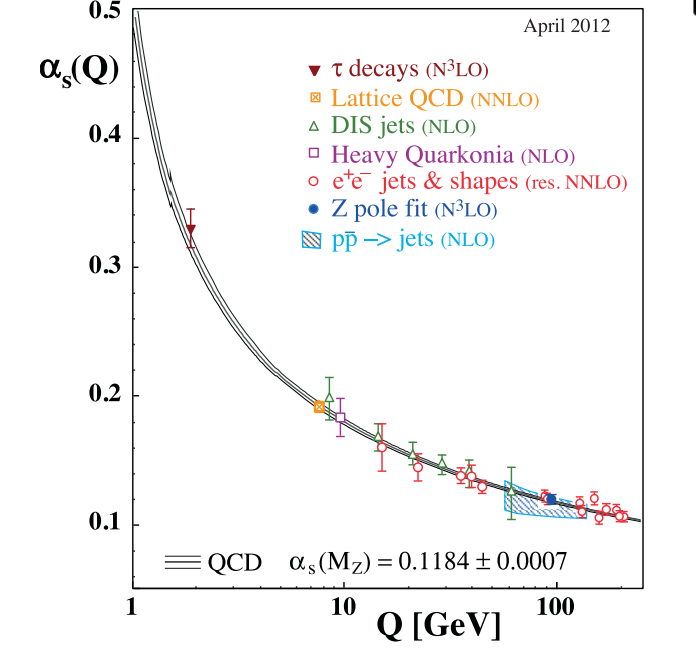
\includegraphics[width=\textwidth]{fig/thry/RunningAlpha.png}
\caption{Summary of measurements of $\alpha_S$ as a function of the respective energy scale, $Q$, from Ref.~\cite{PDG}. The respective degree of QCD perturbation theory used in the extraction
of $\alpha_S$ is indicated in brackets (NLO: next-to-leading order; NNLO: next-to-next-to leading order; res. NNLO: NNLO matched with resummed next-to-leading logs;
N3LO: next-to-NNLO).}
\label{fig:alphas}
\end{figure}
\subsubsection{Parton distribution functions}

In high energy scattering, the proton cannot be modeled as three free non-interacting quarks in a bag; the internal partonic structure of the proton must be considered~\ref{PDG, Campbell:2006wx}. The three \emph{valence} quarks exist in a sea of virtual quark-antiquark pairs that arise from the gluons holding the quarks together. All of these partons contribute to the internal structure of the proton. The proton can be modeled as a collection of these partons that are each carrying a fraction $x$ of the proton's momentum. The \emph{Parton Distribution Function} (PDF) describes the internal proton structure via normalized momentum distribution functions of the constituent partons

 Since the PDFs deal with the non-perturbative regime of QCD, PDFs must be determined by global fits to experimental measurements of deep inelastic and other hard-scattering processes. PDFs derived from measurements of one process can be used for predictions in a different process. For example, positron-proton scattering data from the HERA experiment can be used to make predictions for proton-proton collision at the LHC. One common PDF set used at the LHC, called MSTW, is shown in Figure~\ref{fig:mstw}.

PDF measurements depend on the scale of the hard probe, so theoretical calculations are needed to evolve the PDFs between experimental data points. The differential equations governing the $\mu^2$ dependence of the PDFs are called the DGLAP equations and are derived in Ref.~\cite{Altarelli:1977zs}. Much like the RGE introduces an arbitrary $\mu_R$, the DGLAP equations introduce a factorization scale $\mu_F$ to absorb the divergences from soft parton emissions. To avoid unnaturally large logarithms in the pertubative expansion,  $\mu_F$ and $\mu_R$ are usually assumed to be equal and of the order of the typical momentum scales of the hard scattering process. The theoretical uncertainty from the arbitrary choice of $\mu_F$ and $\mu_R$ is usually evaluated by repeating the calculation with the scale doubled and halved.
\begin{figure}[h]
\centering
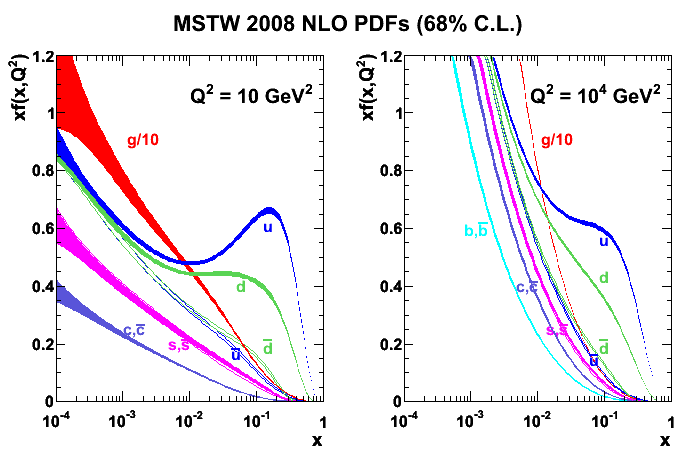
\includegraphics[width=0.8\textwidth]{fig/thry/mstw.png}
\caption{MSTW 2008 NLO PDFs at $Q^2= 10 \gev^2$ and $Q^2= 10^4 \gev^2$~\cite{mstw}.}
\label{fig:mstw}
\end{figure}


\subsubsection{Factorization}


Because of the scale dependence of QCD, interactions can be separated into two regimes, with the transition around the QCD confinement scale, $\Lambda_{QCD} \sim 200$ MeV, the energy at which QCD because non-perturbative. At low energy, $\alpha_S$ is of order unity, so perturbative expansion is not possible. The quarks are bound together by soft gluon exchange into a hadron. At scales far above the QCD confinement scale, the partons can be considered free objects and can be treated with perturbative expansion.

The hard scatter interaction with momentum transfer $Q$ occurs on a time scale that goes as $\tau \sim 1/Q$ which is much larger than the time scale of interactions between protons $\tau \sim 1/\Lambda_{QCD}$. This fact allows high energy proton collisions to be \textit{factorized} into two independent processes: the PDF, which a phenomelogical description of the momentum distribution among the partons inside the proton which depends only on the momentum scale, and the partonic cross section $\hat{\sigma}$, which uses perturbative QCD to determine the calculates the scatter of the hard probe from one of the free partons inside the proton.


Specifically, the hadronic cross-section for a particular process can be written the weighting of the subprocess cross section with the PDFs $f_{q/A}(x)$ extracted from deep inelastic scattering experiments\cite{Campbell:2006wx}:
\begin{eqnarray}
\sigma(AB\rightarrow X) &=& \int dx_a dx_b \,f_{a/A}(x_a,\mu_F^2) f_{b/B}(x_b,\mu_F^2) \hat{\sigma}_{ab \rarrow X} \nonumber \\
&=& \int dx_a dx_b \,f_{a/A}(x_a,\mu_F^2) f_{b/B}(x_b,\mu_F^2) \,\times\,[\sigma_0 + \alpha_{S}(\mu_R^2)\sigma_1 + ...]
\label{eq:ab}
\end{eqnarray}
which is diagramatically represented in Figure~\ref{fig:factorize}. The partonic cross-section can be pertubatively expanded in powers of the strong coupling constant $\alpha_S$ for some renormalization scale $\mu_R$. The PDF $f_{a/A}(x_a,\mu_F^2)$ gives the probability that a proton with momentum $p_A$ contains a parton $a$ with momentum $p_a$. This function depends only on the fraction of the proton momentum distributed to parton $a$, $x_a \equiv p_a/p_A$, and the factorization scale $\mu_F$. 
\begin{figure}[h]
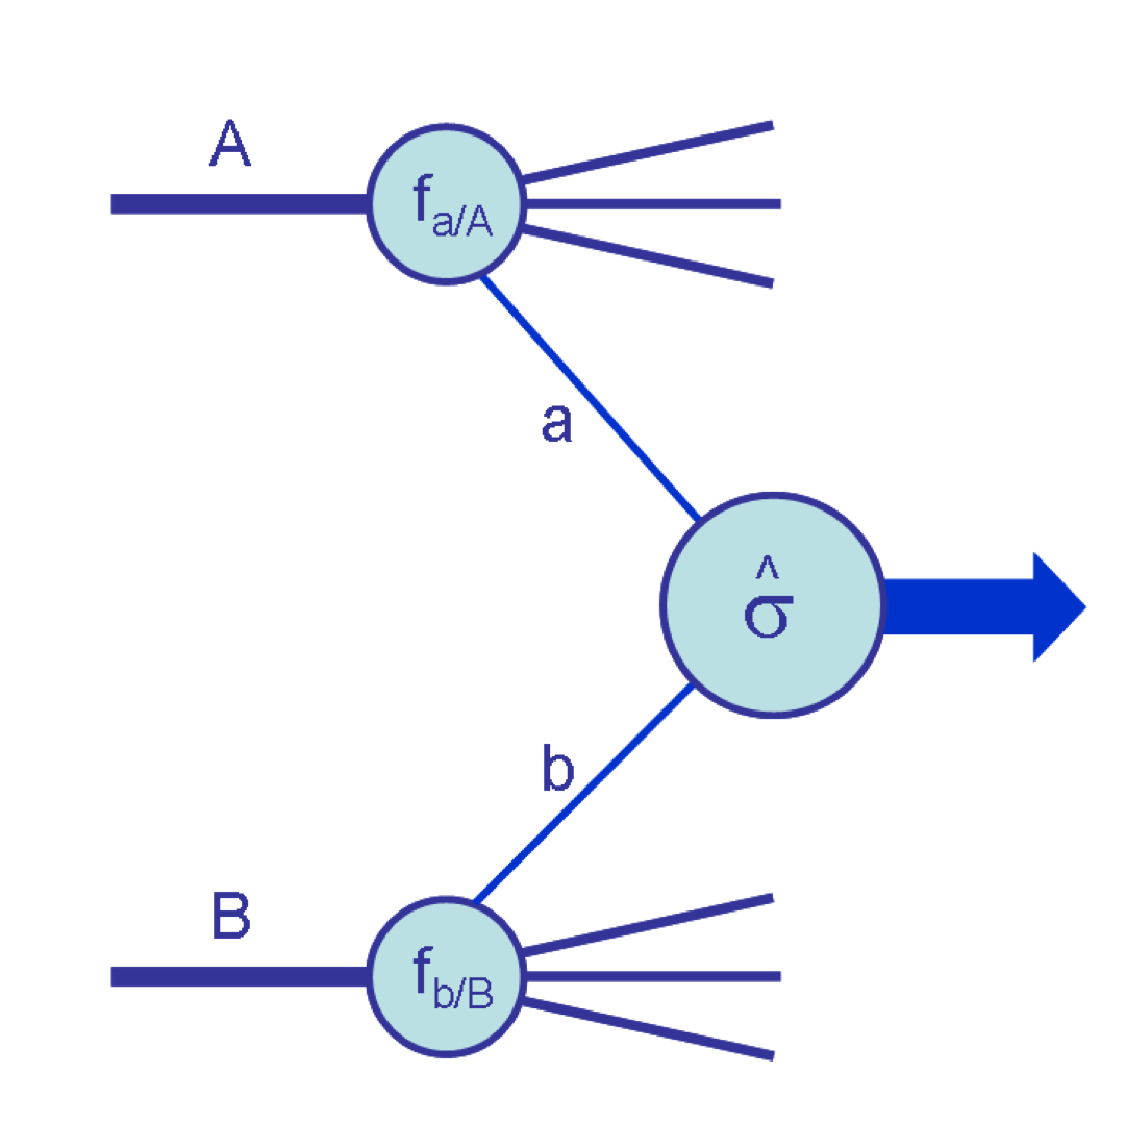
\includegraphics[width=0.9\textwidth]{fig/thry/Factorize.pdf}
\caption{Diagram from Ref.~\cite{Campbell:2006wx} illustrating the structure of a generic hard scattering process of two incoming partons $A$ and $B$ with PDFs $f_{a/A}$ and $f_{b/B}$.}
\label{fig:factorize}
\end{figure}










\section{Top quark physics}
The top quark was first discovered at Fermilab in 1995~\cite{Abe:1995hr}\cite{Abachi:1995iq}. As the heaviest known fundamental particle, the top quark is an important probe of the SM and extensions of the SM. Before the LHC, the Tevatron provided the only experimental observation of the top. The LHC produces a top quark every few seconds, about a hundred times more frequently than the Tevatron. This signifigant increase in statistics allows precision measurements of the top at the LHC, which is sometimes called a ``Top Factory.'' 

Because of its large mass, the top quark plays a special role in the SM. The top mass is about the same as a gold atom nucleus, 40 times larger than the next heaviest quark and $10^5$ times heavier than the lightest quark. The mass of the top quark has been precisely measured in different decay channels at both the LHC and the Tevatron. Figure~\ref{fig:topmass} shows a recent summary of these measurements, which can be combined to give a world average of $173.34 \pm 0.76$ for the top quark mass.

 The top has a very short lifetime ($\sim 5 \e{-25}$ s), so it is the only quark that decays before it can form a hadron with other quarks. This unique property means that the top is the only ``bare'' quark that can be accessed experimentally.



\begin{figure}[h]
\centering
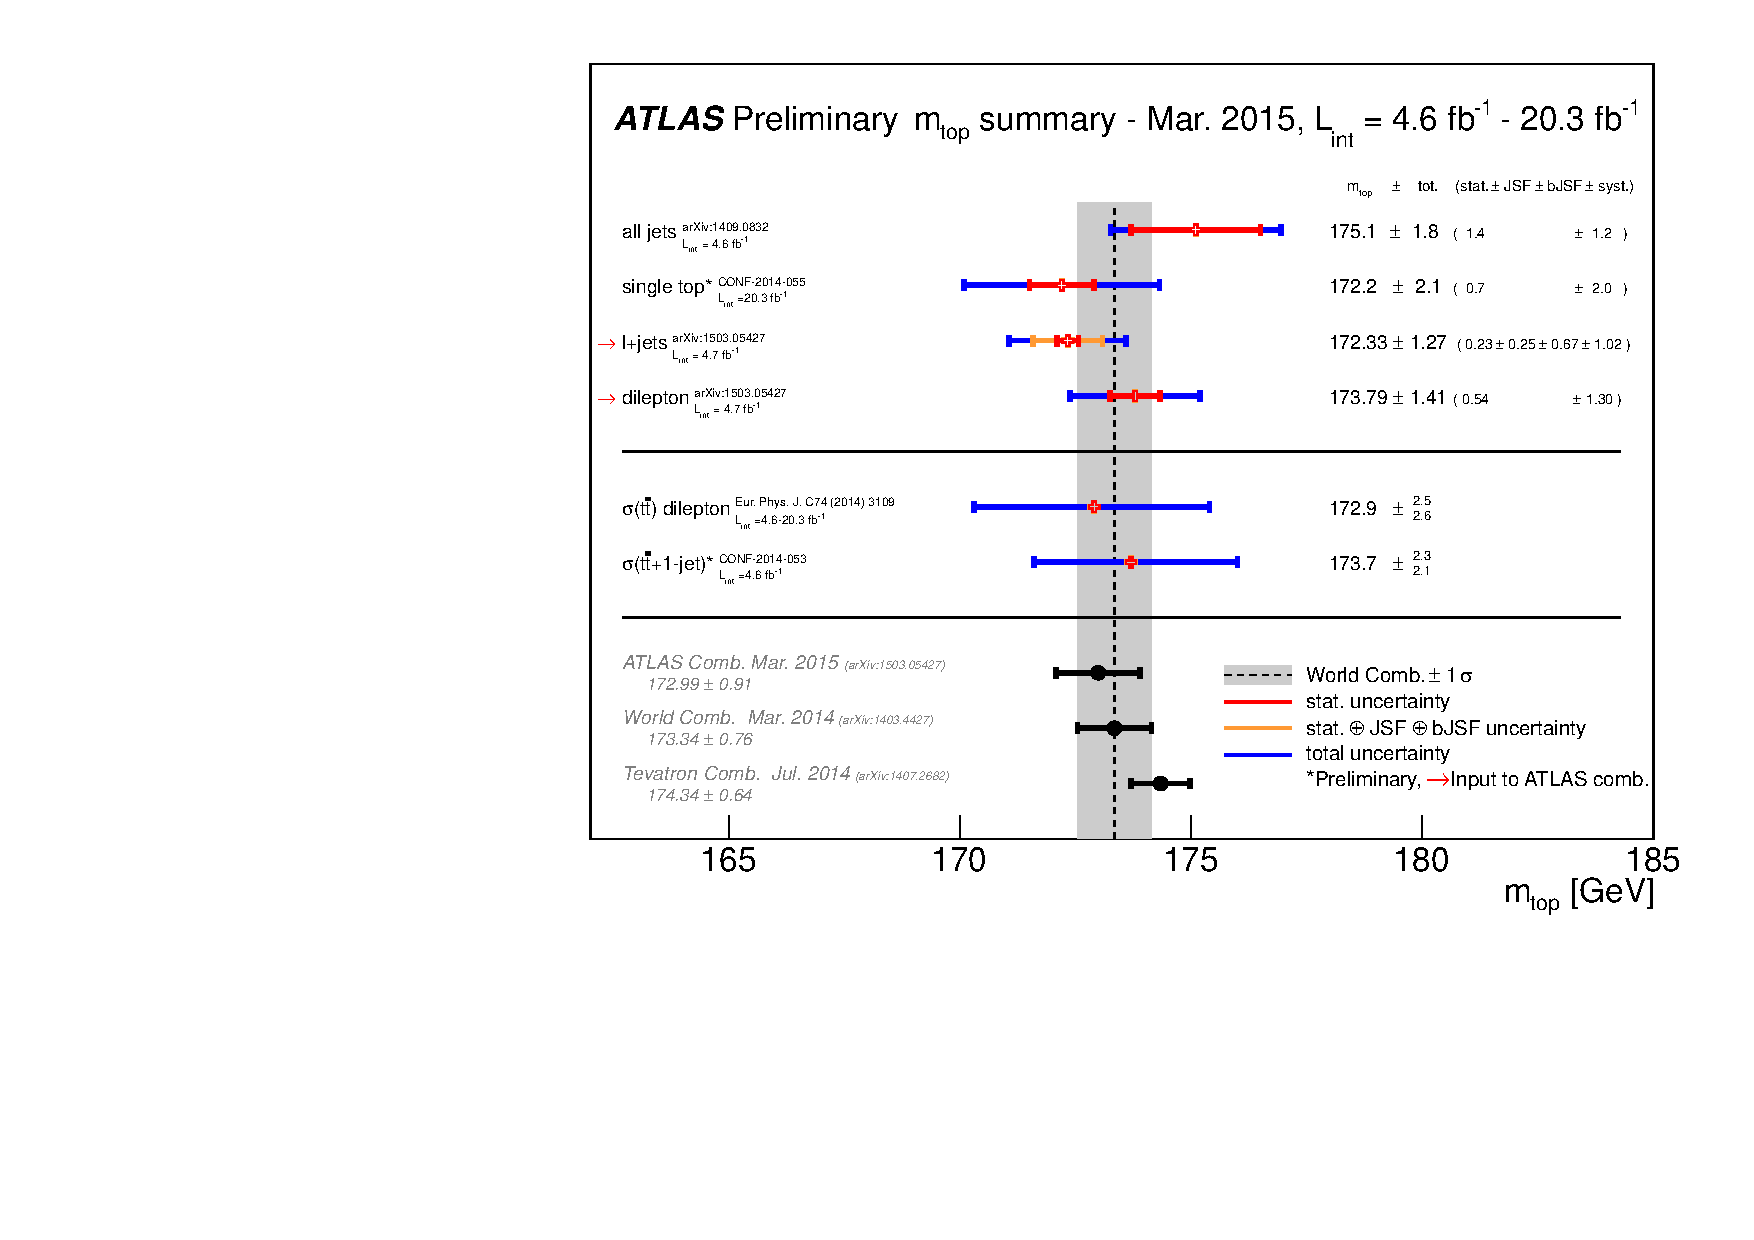
\includegraphics[width=0.8\textwidth]{fig/thry/mtopSummaryAll.pdf}
\caption{Summary of the ATLAS direct $m_{top}$ measurements. The results are compared with the ATLAS, Tevatron and Tevatron+LHC $m_{top}$ combinations. For each measurement, the statistical uncertainty, the sum of the remaining uncertainties are reported separately.}
\label{fig:topmass}
\end{figure}

\subsection{Top quark production at the LHC}

In $pp$ collisions at the LHC, top quarks are mainly produced in pairs through the QCD processes  $gg \rightarrow \ttbar$ and $q\bar{q} \rightarrow \ttbar$. The Feynman diagrams for these processes are shown in Figure~\ref{fig:ttdiag}. At Tevatron with $p\bar{p}$ collisions, \ttbar production was dominated by quark annihilation ($\sim 85$\%). At the LHC, the higher collision energy and lack of valence anti-quarks in the proton result in gluon-fusion dominated \ttbar production ($\sim 85$\%)~\cite{PDG}. The total \ttbar cross-section has been computed at next-to-next-to leading order (NNLO) with next-to-next-to-leading-log soft gluon resummation (NNLL) in Ref.~\cite{Czakon:2013goa} with a final theoretical uncertainty of $\sim 3 \%$ and found to agree with experimental measurements. Figure~\ref{fig:ttxsec} compares this calculation with measurements made at both in the LHC and Tevatron in various decay channels.

\begin{figure}[h]
\centering
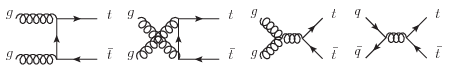
\includegraphics[width=0.8\textwidth]{fig/thry/fig_ttbar.png}
\caption{Feynman diagrams for \ttbar production at leading order QCD}
\label{fig:ttdiag}
\end{figure}

\begin{figure}[h]
\centering
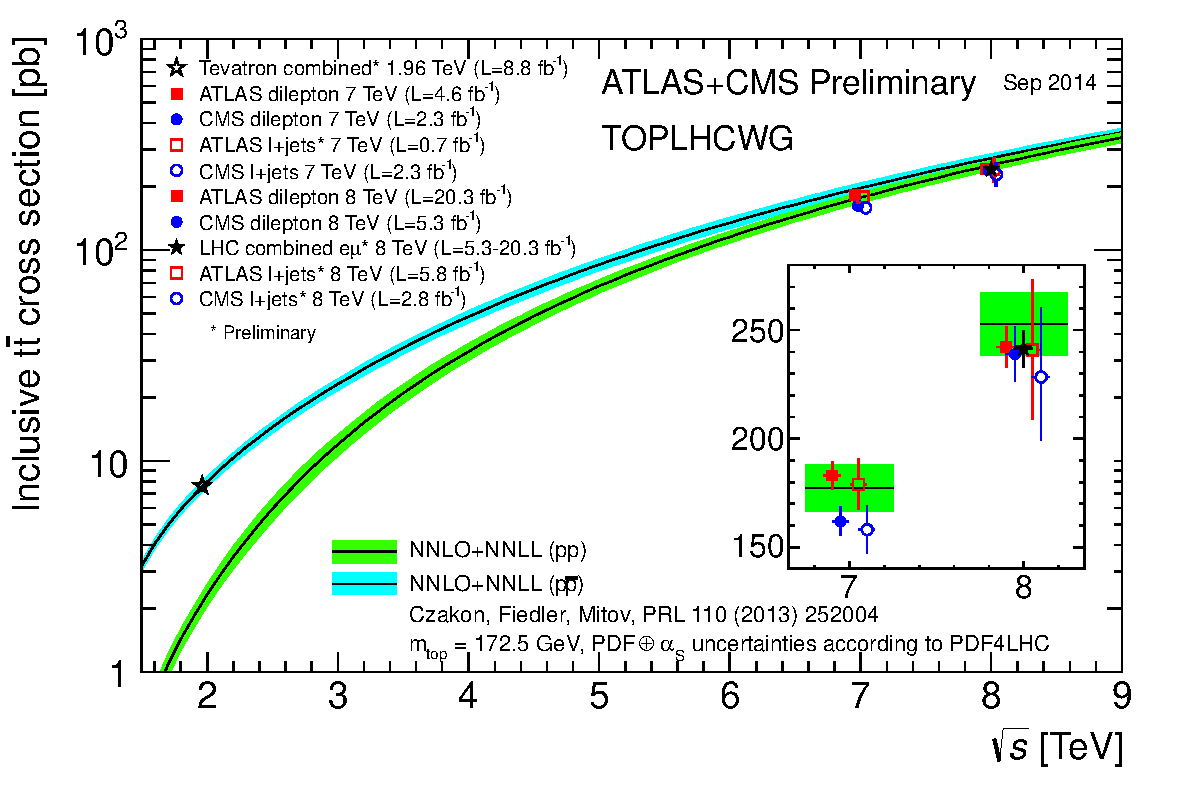
\includegraphics[width=0.8\textwidth]{fig/thry/tt_xsec_vsroots.pdf}
\caption{Summary of LHC and Tevatron measurements of the top-pair production cross-section as a function of the centre-of-mass energy compared to the NNLO QCD calculation complemented with NNLL resummation (top++2.0). The theory band represents uncertainties due to renormalisation and factorisation scale, parton density functions and the strong coupling. The measurements and the theory calculation is quoted at $m_{top}$=172.5 GeV. Measurements made at the same centre-of-mass energy are slightly offset for clarity.}
\label{fig:ttxsec}
\end{figure}

Top quarks can also be produced singly via electroweak processes. Because the weak coupling is much smaller than the strong coupling, fewer top quarks are produced singly than in pairs. The Feynman diagrams for single top production are shown in Figure~\ref{fig:tdiag}. Single production can mediated by virtual $s$-channel and $t$-channel $W$-bosons. These production channels provide sensitivity to physics beyond the SM. Single tops are also produced in association with a $W$-boson ($Wt$-associated production). While negligible at the Tevatron, at the LHC, $Wt$-associated production provide a sizeable contribution to single top production. The inclusive cross-section for $s$-channel, $t$-channel and $Wt$-associated single top production has been computed to NNLO. This calculation is compared with the ATLAS experimental measurements of each channel in Figure~\ref{fig:txsec}.

The calculation of $Wt$ at NLO is non-trivial since the NLO $Wt$ production process interferes with the LO \ttbar\ production\cite{White:2009yt}. Because of this interference, NLO $Wt$ is not well-defined and a prescription must be adopted to deal with the interference to calculate $Wt$ production beyond LO. The two most common prescriptions are \emph{diagram removal} (DR) and \emph{diagram subtraction} (DS). In the DS method, the resonant \ttbar\ effects are removed at the cross-section level.  In the DR method, the resonant \ttbar\ effects are removed from $Wt$ at amplitude level. The difference between these two methods essentially corresponds to the interference between \ttbar\ and $Wt$ production. Due to this complication, the $Wt$ is treated as part of the signal, rather than subtracted as background, in this thesis. This procedure is discussed in later chapters.


\begin{figure}[h]
\centering
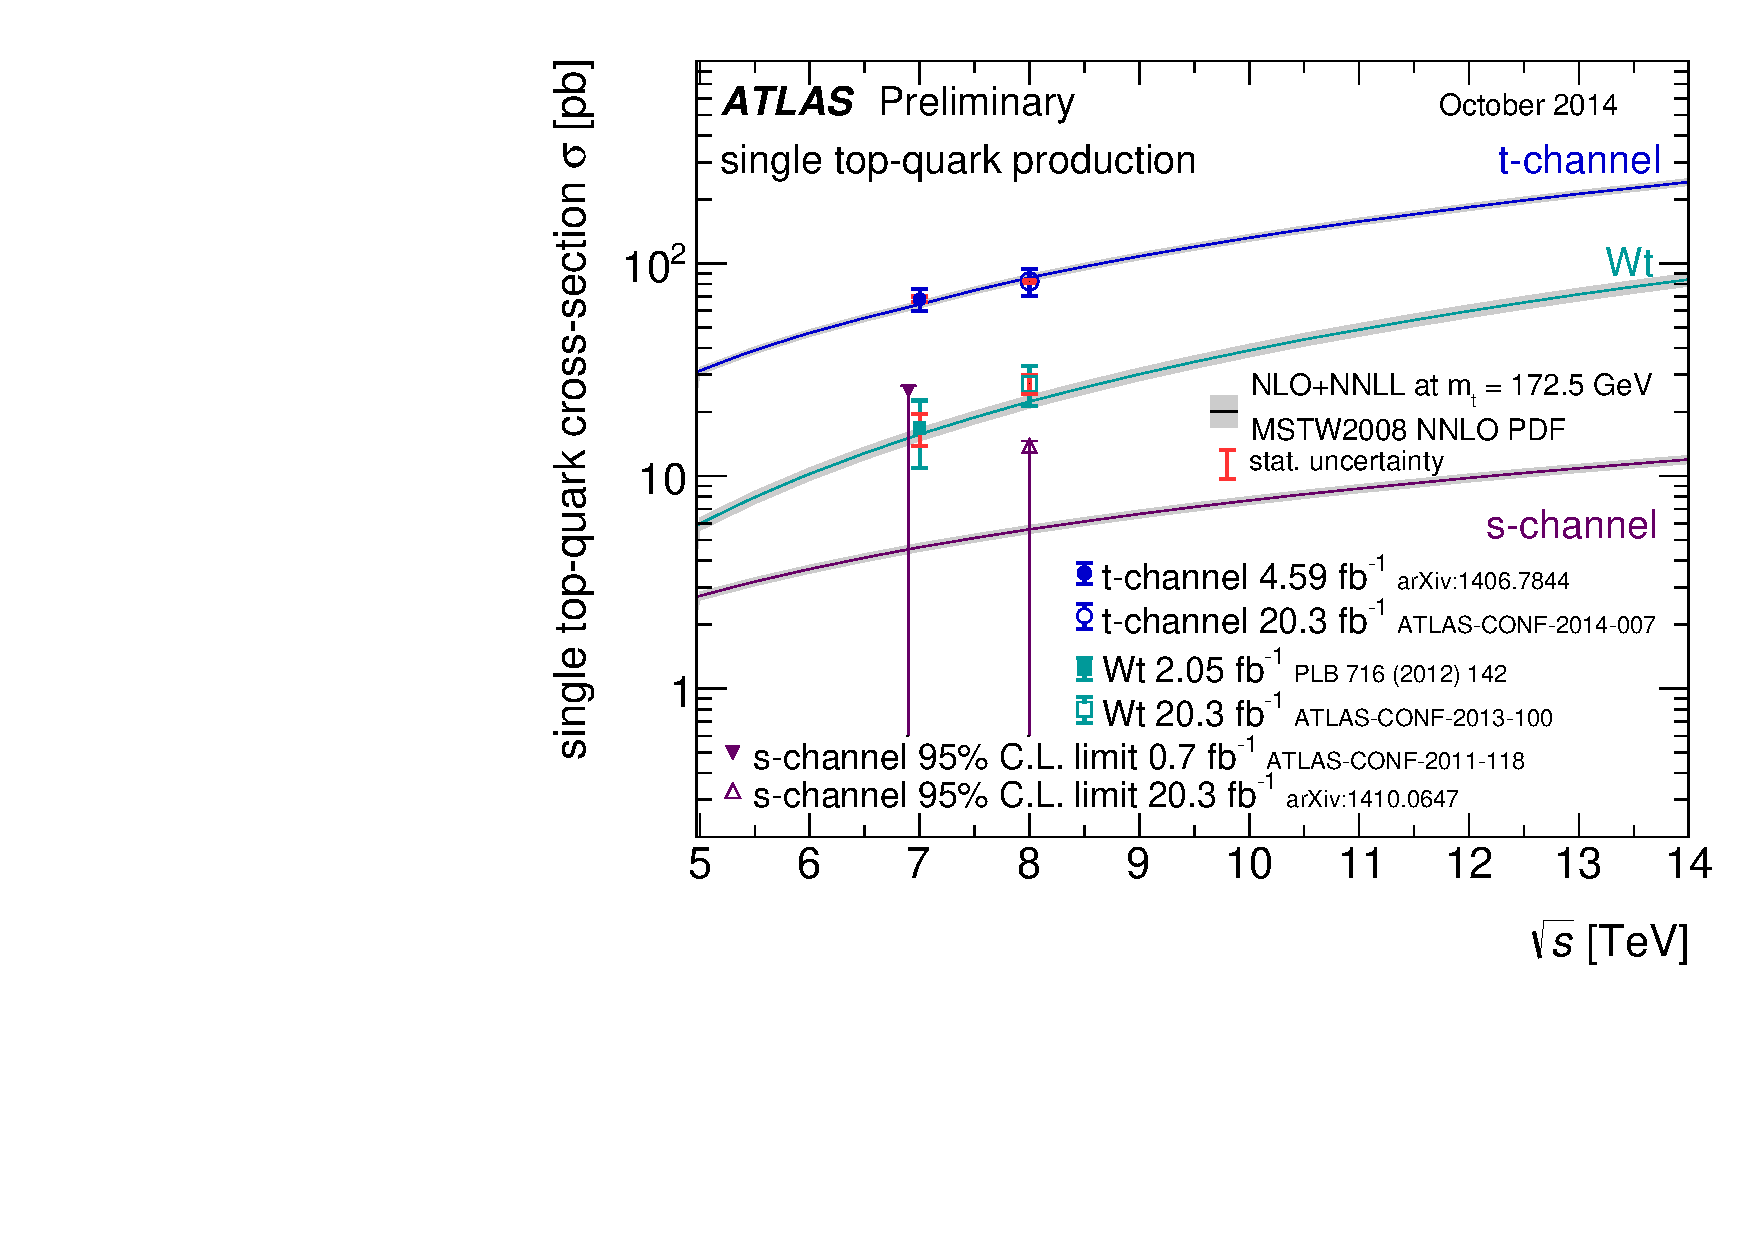
\includegraphics[width=0.8\textwidth]{fig/thry/singletop_allchanvsroots_ATLASonly.pdf}
\caption{Summary of ATLAS measurements of the single top production cross-sections in various channels as a function of the center of mass energy compared to a theoretical calculation based on NLO QCD complemented with NNLL resummation. For the $s$-channel only an upper limit is shown.}
\label{fig:txsec}
\end{figure}
\begin{figure}[h]
\centering
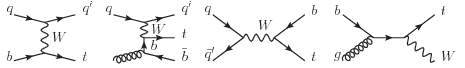
\includegraphics[width=0.8\textwidth]{fig/thry/fig_singletop.png}
\caption{Feynman diagrams for single top quark production at leading order QCD. From left to right: $t$-channel production as flavor excitation; $t$-channel production as $W$-gluon fusion; $s$-channel production; $Wt$-channel production.}
\label{fig:tdiag}
\end{figure}

\subsection{Top quark decays}
In the SM, the top quark decays to a $W$ boson and a down-type quark: $t \rightarrow qW$ where $q=b,s,d$. The rate of each of these decays is proportional to the square of the Cabibbo-Kobayashi-Masakawa (CKM) matrix, $|V_{tq}|^2$~\cite{PDG}. Measured from experiment, the CKM matrix governs quark mixing in flavor-changing weak decays.



Weak hadron decays and the unitiary of the CKM matrix constrain the value of $0.9990 < |V_{tb}| < 0.9992$ at the 95\% C.L~\cite{Chetyrkin:1999ys}. Top quarks nearly always decay with $t \rightarrow Wb$. Figure~\ref{fig:tdec} shows the decay of a top quark, both hadronically and leptonically.

\begin{figure}[h]
\centering
\subfloat{
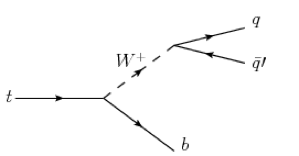
\includegraphics[width=0.8\textwidth]{fig/thry/ttdecqq.png}}
\subfloat{
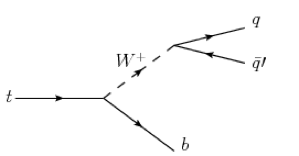
\includegraphics[width=0.8\textwidth]{fig/thry/ttdecqq.png}}
\caption{Feynman diagrams for top quark decay. On the left, the top quark is shown decaying hadronically. On the right, the top quark is shown decaying leptonically.}
\label{fig:tdec}
\end{figure}

Experimentally, the decay modes of \ttbar are distinguished by the decay of the two $W$-bosons:
\begin{description}
\item[All hadronic] Both $W$ bosons decay to quark pairs: $\ttbar \rightarrow WbWb \rightarrow bbqqqq$. Because there are 6 quarks in the final state, this channel has a large multi-jet background, which can be difficult to subtract. 

\item[Semi-leptonic] One $W$ boson decays to a quark pair and the other decays to a lepton and neutrino: $\ttbar \rightarrow WbWb \rightarrow bbqq \ell \nu$. This channel can be further categorized by lepton flavor.


\item[Dileptonic] Both $W$ bosons decay to leptons: $\ttbar \rightarrow WbWb \rightarrow bb\ell \nu\ell \nu$. Though the dilepton channel has the fewest events, it often provides least background.


\end{description} 
This thesis uses \ttbar\ events from the dilepton $e\mu$ channel. The minimal background allows more robust generator comparisons.
\section{Beyond the SM}
In addition to providing a test of the SM, the top quark may also provide a window to physics at higher energy scales beyond the SM.

The top quark is important in aesthetic problem with the Higgs mass known as the hierarchy problem or fine tuning. The Higgs mechanism provides an explanation for electroweak symmetry breaking and acquisition of mass by other SM particles. As a scalar particle, the Higgs receives higher-order corrections to its physical (measured) mass from interactions with fermions, gauge bosons and itself. These corrections are on the order of the Planck scale, $\mathcal{O}(\Lambda^2 \approx 10^{30-38} \gev)$, while the observed mass is class to the electroweak scale, $\mathcal{O}(100 \mev)$. Thus, in order to obtain the observed mass without introducing new physics, there must be an unnatural canceling. Since the dominant higher-order correction to the Higgs mass comes from the top, precisely measuring the top's mass and other properties may provide insight to this problem. 

In addition to the hierarchy problem, there are several other open questions which cannot be explained by the SM. The SM does not account for the 85\% of our universe made up of \textit{dark matter} particles, or provide an explanation for the observed asymmetry between matter and anti-matter. The SM also does not account for the observed non-zero mass of neutrinos or have a way to incorporate gravitational interactions.

Theorists have formulated many extensions to the SM that address these puzzles. Perhaps the most widespread, Supersymmetry (SUSY)~\cite{susy} proposes an additional superpartner for every particle in the SM. SUSY is especially popular because it naturally contains a light, stable, neutral dark matter candidate and solves the hierarchy problem. Diagrams from superpartners remove the need to fine tune the Higgs mass. Since SUSY has not been observed, the superpartners of SM particles must have different masses, and SUSY has to be a broken symmetry. However, in order to satisfactorily solve the hierarchy problem, the superpartners with the largest contributions to the Higgs mass must be $\mathcal{O}(\tev)$. This means that they should be discoverable at the LHC.

Another popular SM extension, called the Randall-Sundrum model~\cite{Lillie:2007yh}, posits an extra dimension in which gravity would propagate. This model includes a new particle, a Kaluza-Klein gluon, that propagates into the extra dimension and decays into a top quark pair.
%COULD ADD MORE ABOUT WHY SIGNALS IMPOR. See a thesis

Many of the signals for new physics are dominated by the top quark since heavier particles are more sensitive to higher energy scales.  The top pair production analyzed in this thesis is important as a background for \ttbar resonances~\cite{ATLAS-CONF-2015-009} and other searches~\cite{Aad:2014kra}.



% \section{QCD in hadron-hadron collisons}
% The protons collided at the LHC are composite objects made of point-like quarks held together by soft gluon emissions. Because of the asymptotic freedom of QCD, $\alpha_S$ is of order unity at the scale of these emissions within the proton, but as the scale of emissions increase $\alpha_S$ quickly drops. Then, at scales far above the QCD confinement scale ($\Lambda_{QCD} \sim 200$ MeV, the energy at which QCD because non-perturbative), the protons can be considered free objects. The hard scatter interaction with momentum transfer $Q$ occurs on a time scale that goes as $\tau \sim 1/Q$ which is much larger than the time scale of interactions between protons $\tau \sim 1/\Lambda_{QCD}$. This fact allows high energy proton collisions to be \textit{factorized} into two independent processes: the Parton Distribution Function (PDF), which describes the momentum distribution among the partons inside the proton and depends only on the momentum scale, and the partonic cross section $\hat{\sigma}$, which uses perturbative QCD to determine the calculates the scatter of the hard probe from one of the free partons inside the proton.

% PDF STUFF

% Then, the final \ttbar  cross section ($\sigma_{\ttbar}$) is a convolution of the partonic cross section ($\qqbar, qq \rightarrow \ttbar$)and the parton distribution functions (PDFs)~\cite{Moch:2008qy}:

% \begin{equation}
% \sigma_{\ttbar}(s, m_{t}) = \sum_{i, j} \int^1_0 dx_i  \int^1_0 dx_j f_i \left(x_i, \mu_F^2 \right) f_j\left(x_j, \mu_F^2 \right) \times \hat{\sigma}_{ij} \left( \hat{s}, m_{t}, \alpha_s \left(\mu_R \right), \mu_R,  \right)
% \end{equation}

% DISCUSSION OF GLUON GLUON ETC AT LHC

% At the LHC, $qg$ scattering occurs with the highest parton luminosity but the partonic cross-section $\hat{\sigma}_{qg}$ is smaller than either $\hat{\sigma}_{gg}$ or $\hat{\sigma}_{qq}$. The largest contribution for top pair production at the LHC comes from gluon-gluon fusion, due to the combination of a large partonic cross-section and the second largest parton luminosity. The second largest contribution comes from quark-antiquark annihilation. At NLO QCD, the total \ttbar\ production at the LHC comprises approximately 90\%

% At the Tevatron, a previous $p\bar{p}$ collider with lower energy, \ttbar production was 

% AHHH REPETITIVE










\chapter{Phenomenology at the LHC}
\label{ch:pheno}
\section{Predictions for hadron colliders}
The basic principles discussed above are employed in Monte Carlo simulation to allow comprehensive predictions for various kinematic distributions of the final state products in hadron collisions.
\subsection{Parton distribution functions}

Since the PDFs are not calculable from first principle, they are derived by fitting experimental data and then serve as input to MC calculations. 

PDFs are generally extracted from data at a particular value of momentum transfer, characteristic of the experiment sourcing the data, and then extrapolated to other $Q^2$ values. In addition, different processes are generally most sensitive to a particular PDF over a particular range of proton momentum fraction values. For example, data from Deep Inelastic Scattering (DIS) experiments, where the probes are leptons, can be used to directly constrain only quark PDFs. Information about the gluon PDF can then be inferred indirectly since the DGLAP evolution of quarks leads to generating gluons and vice versa.
Given this constraint, the best estimate of the PDFs are obtained by combining data from multiple experiments and processes into global fits. This is done by 3 PDF fitting collaborations: CTEQ~\cite{Lai:2010CT10}, MSTW~\cite{Martin:2009MSTW} and NNPDF~\cite{Ball:2012NNPDF}. The current knowledge of the proton PDFs according to NNPDF is shown in Figure~\ref{fig:pdfs}. At large-$x$, most of the momentum is carried by the valence quarks and up-type quarks account for about twice the momentum as compared to down-quarks. Comparing the left and right subfigures confirms that as the probe becomes more energetic, a higher fraction of the proton momentum is found in the sea quarks and gluons. 
\subsection{Hard collision simulation}
Description of the partonic cross-section lies in the domain of perturbative QCD and therefore lends itself to analytic calculations. Currently there exist Monte Carlo based programs that can perform these calculations automatically at both the leading order (LO) and next-to-leading order (NLO) in $\alpha_S$. The leading order matrix element is always positive making it possible to implement the calculations via the Monte Carlo method. On the other hand, at NLO there are real and virtual divergent contributions, due to soft and collinear emissions, that must cancel in order to obtain finite results. This cancellation is guaranteed for inclusive observables like the total cross-section, but not so for observables like parton multiplicity~\cite{pdgbook}. In general, perturbative QCD can only provide sensible results for infrared and collinear (IRC) safe observables, which are observables insensitive to the addition of infinitely soft particles or the splitting of a particle into two collinear emissions.

\subsection{Parton shower and hadronization}

\subsection{Merging fixed-order with parton shower}

\section{Monte Carlo generators}
particle level v. reco level

types of generators

\section{Jets}
why antikt is good

\chapter{The ATLAS detector and the LHC}
\label{ch:atlas}
\section{The Large Hadron Collider}
The Large Hadron Collider (LHC)`\cite{cern-faq} is the largest and most powerful particle collider that has ever been built. Construction of the LHC involved a collaboration of more than 10,000 scientist from more than 100 countries and was completed in 2008, after a decade of work. The cost of the machine alone is about 5 billion USD (3 billion Euro). The main goal of the LHC is to investigate unsolved questions in our current understanding of particle physics, such as the details of the Higgs mechanism, the existence of new particles from SUSY or extra dimensions and the source of dark matter and dark energy.

The European Organization for Nuclear Research (CERN) built the LHC in a tunnel underneath the border of France and Switzerland, near the city of Geneva. The LHC occupies a large tunnel 27 km in circumference that was originally constructed in the 1990s for the Large Electron Positron collider (LEP). Hadrons (either protons or ions) are accelerated and focused into two beams traveling in opposite directions around this tunnel. These beams then collide with very high energy at each of the four collision points along the ring where the paths of the two beams intersect. Each collision point is home to one of the four main LHC experiments: A Large Ion Collider
Experiment (ALICE)~\cite{cern-jinst-alice}, ATLAS~\cite{cern-jinst-atlas}, the Compact Muon Solenoid (CMS)~\cite{cern-jinst-cms}, and the Large Hadron Collider beauty (LHCb) experiment~\cite{cern-jinst-lhcb}. ALICE is a detector that looks at collisions of lead ions to study the properties of quark-gluon plasma. ATLAS is a general-purpose detector that looks for a wide range of possible new types of physics, including the Higgs boson, SUSY, and extra dimensions. CMS is an additional general-purpose detector, designed and run independently from ATLAS, but with the same goals in mind. LHCb is a detector specially designed to study the asymmetry between matter and anti-matter in the interactions of B-particles. Figure~\ref{fig:lhc-exp} shows a aerial view diagram with the locations of these four experiments along the LHC ring. The location of the LHC ring in relation to the city of Geneva and the French-Swiss border is also illustrated.

\begin{figure}[tp]
  \centering
  \includegraphics[width=0.90\textwidth]{fig/atlas/lhc-surface.jpg}
  \caption{The location of the four main LHC experiments: ALICE, ATLAS, CMS and LHCb. The LHC tunnel is 27 km in circumference, situated underneath the border of France and Switzerland, near the city of Geneva, as shown~\cite{atlas-surface}.}
  \label{fig:lhc-exp}
\end{figure}


\subsection{Accelerator Complex}
A succession of machines known as the \emph{accelerator complex} accelerate particles to increasingly higher energies~\cite{cern-jinst-lhc}. A diagram of the accelerator complex is shown in Figure~\ref{fig:lhc-chain}. First, an electric field is used to strip protons from atoms in a simple bottle of hydrogen gas. Then, the first accelerator in the chain, Linac 2, accelerates protons to 50 \mev. Next, the beam is injected into the Proton Synchrotron Booster (PSB) and then the Proton Synchrotron (PS), which accelerate the protons to 1.4 \gev and 25 \gev respectively. After that, the Super Proton Synchrotron accelerates the protons to 450 \gev. The last step in the chain is the LHC; from the SPS, protons are transferred into the two beam pipes of the LHC and accelerated in opposite direction. Filling each of the rings of the LHC takes 4 minutes and 20 seconds, and it takes another 20 minutes to accelerate each beam to its final energy of 4 \tev. The same two beams will circle for many hours.

Inside the LHC, the beams travel in opposite directions around separate rings called \emph{beam pipes} (or beamline), which are tubes kept at ultrahigh vacuum. The beams are directed by a collection of very strong superconducting electromagnets, including 1232 dipole magnets and 392 quadrupole magnets. Superconduction requires the magnets to be cooled to -271.3 C. A distribution system of liquid helium keeps the magnets cool. The 15 meter long dipole magnets steer the beams around the ring, while the 5-7 meter long quadrupole magnets focus the beams before collision. 






\begin{figure}[tp]
  \centering
  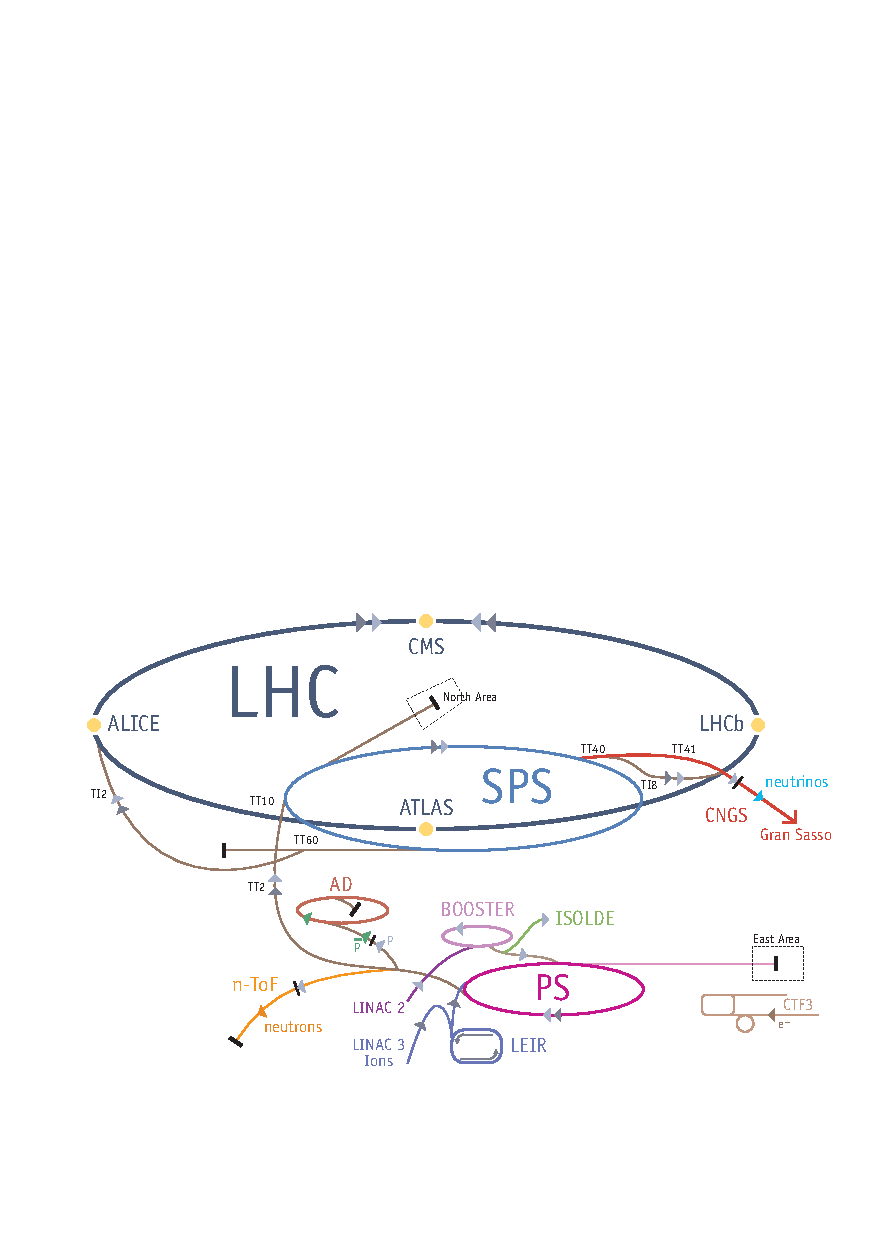
\includegraphics[width=0.90\textwidth]{fig/atlas/accel-chain.pdf}
  \caption{The LHC accelerator complex boosts particles to increasingly higher energies before reaching the LHC. The particle beams are accelerated successively by Linac 2, the Proton Synchrotron Booster (PSB), the Proton Synchrotron (PS), the Super Proton Synchrotron (SPS) and then finally enter the LHC rings~\cite{cern-faq}.}
  \label{fig:lhc-chain}
\end{figure}
\section{Beam conditions}
Due to the Radio Frequency (RF) fields in the accelerating cavities, the proton beams are segmented into groups of protons called \textit{bunches}. Each beam contains 2808 bunches, and each bunch contains 1.7$\times$10$^{11}$ protons. Many protons are included per bunch to maximize the probability of a proton-proton collision for a given bunch crossing. A bunch crossing occurred every 50 nanoseconds during operations in 2012.

Given two equally bunched beams, the \emph{instantaneous luminosity} ($\mathcal{L}$) is given by~\cite{PDG}:
\begin{equation}\label{eqn:lumi}
  \mathcal{L} = f \frac{n_1 n_2}{4\pi \sigma_x\sigma_y},
\end{equation}
where $f=\SI{11245.5}{\hertz}$ is the collision frequency of the LHC beams; $n_{1}$ and $n_{2}$ are the numbers of protons in each beam; and $\sigma_{x}$ and $\sigma_{y}$ are the RMS beam widths in the horizontal (bend) and vertical directions. The maximum instantaneous luminosity of the LHC in 2012 was 7.7$\times$10$^{33}$ cm$^{-2}$ s$^{-1}$.

The instantaneous luminosity must be integrated over time to obtain total luminosity. The beam conditions that go into Equation~\ref{eqn:lumi} change over the duration of a run. The integral over time and varied beam conditions is called the \emph{integrated luminosity} and can be used to relate the number of events $N$ for a given physics process to its cross section $\sigma$:
\begin{equation}\label{eqn:nevt}
  N = \sigma \times \int{\mathcal{L}(t) dt}
\end{equation}
In 2012, the total integrated luminosity of the LHC was 20.3 fb$^{-1}$ with uncertainty of 2.8\% \cite{Lumi}. The cumulative luminosity recorded over the course of 2012 is shown in Figure~\ref{fig:2012lumi}.
\begin{figure}[tp]
  \centering
  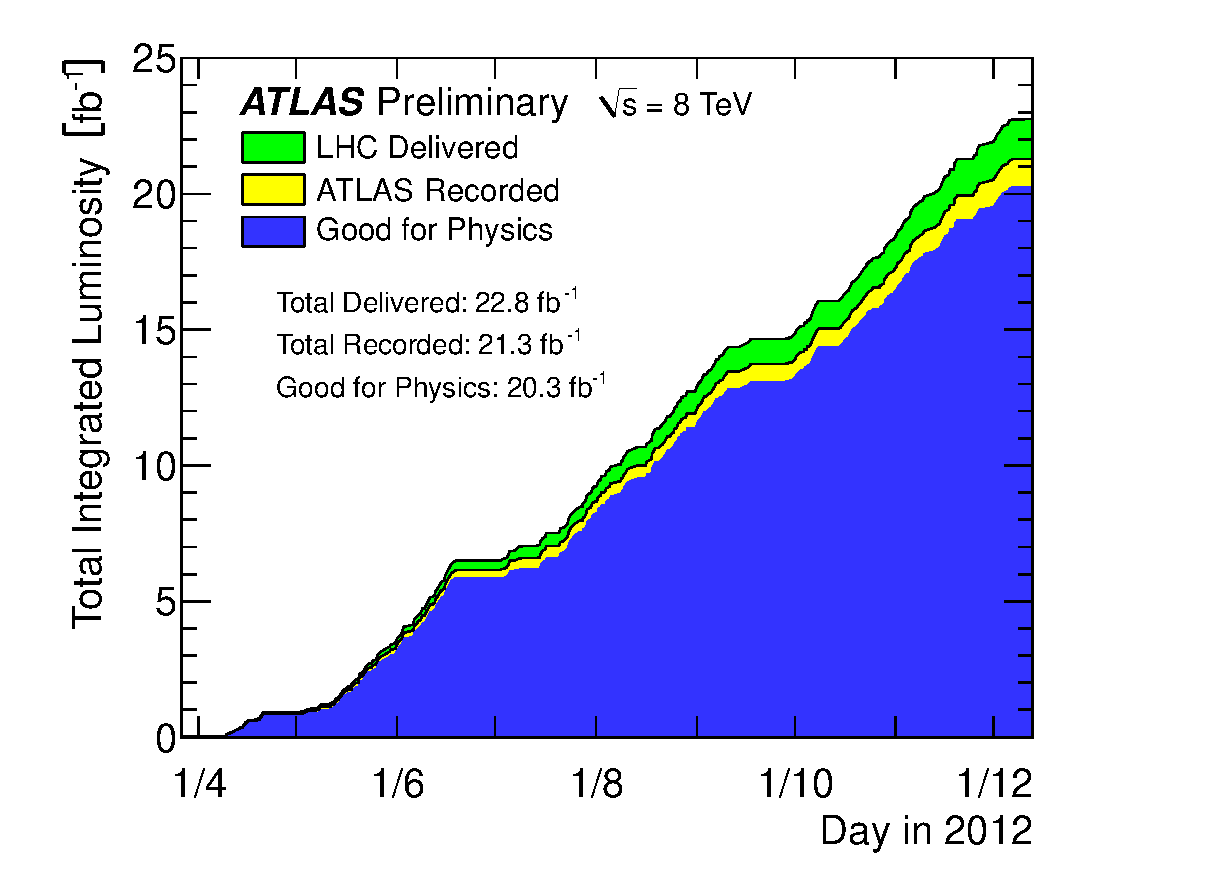
\includegraphics[width=0.90\textwidth]{fig/atlas/intlumivstime2012DQ.eps}
  \caption{Cumulative luminosity versus time delivered to (green), recorded by ATLAS (yellow), and certified to be good quality data (blue) during stable beams and for pp collisions at 8 TeV center-of-mass energy in 2012. Luminosity can be lost due to data acquisition inefficiency or other effects.}
  \label{fig:2012lumi}
\end{figure}

The beam conditions also determine the number of proton-proton interactions that occur in a single bunch crossing. When a single bunch crossing produces multiple separate proton-proton collisions, these events are referred to as \textit{pileup}. Pileup presents a significant challenge since it can rapidly increase the combinatoric complexity of reconstructing events and degrade the performance of the reconstruction algorithms. Figure~\ref{fig:atlas-pileup} shows the mean number of interactions per bunch crossing for 2011 and 2012, demonstrating the substantial increase of pileup events in the latter. Reconstruction challenges were overcome by optimizing the existing reconstruction algorithms, as well as new techniques for subtracting pileup events from the physics of interest~\cite{pileup}. 

\begin{figure}[tp]
  \centering
  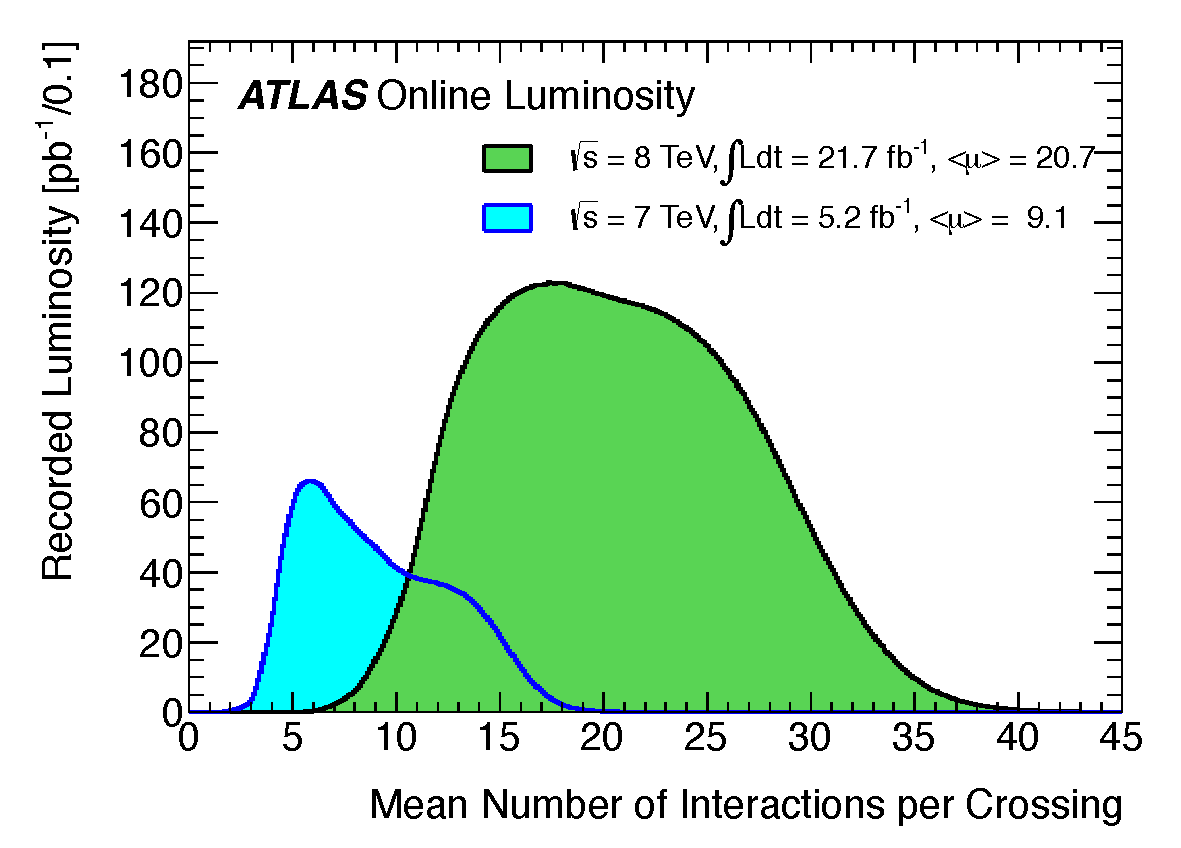
\includegraphics[width=0.90\textwidth]{fig/atlas/pileup.pdf}
  \caption{Luminosity-weight distribution of the mean number of interactions per bunch crossing. Both the full data from the 2011 and 2012 $pp$ runs at the LHC are shown.}
  \label{fig:atlas-pileup}
\end{figure}



\section{Overview of the ATLAS detector}
The ATLAS detector is a general purpose detector centered over one of the four interaction points of the LHC. The detector is cylindrical in shape with a diameter of 25 meters, a length of 46 meters, and a weight of 7,000 tons; it contains around 100 million electronic channels and around 3,000 km of cables. Assembling the detector at CERN took 5 years and was completed in 2008. A schematic rendering of the ATLAS detector is shown in Figure~\ref{fig:atlas-cgi}.
\begin{figure}[tp]
  \centering
  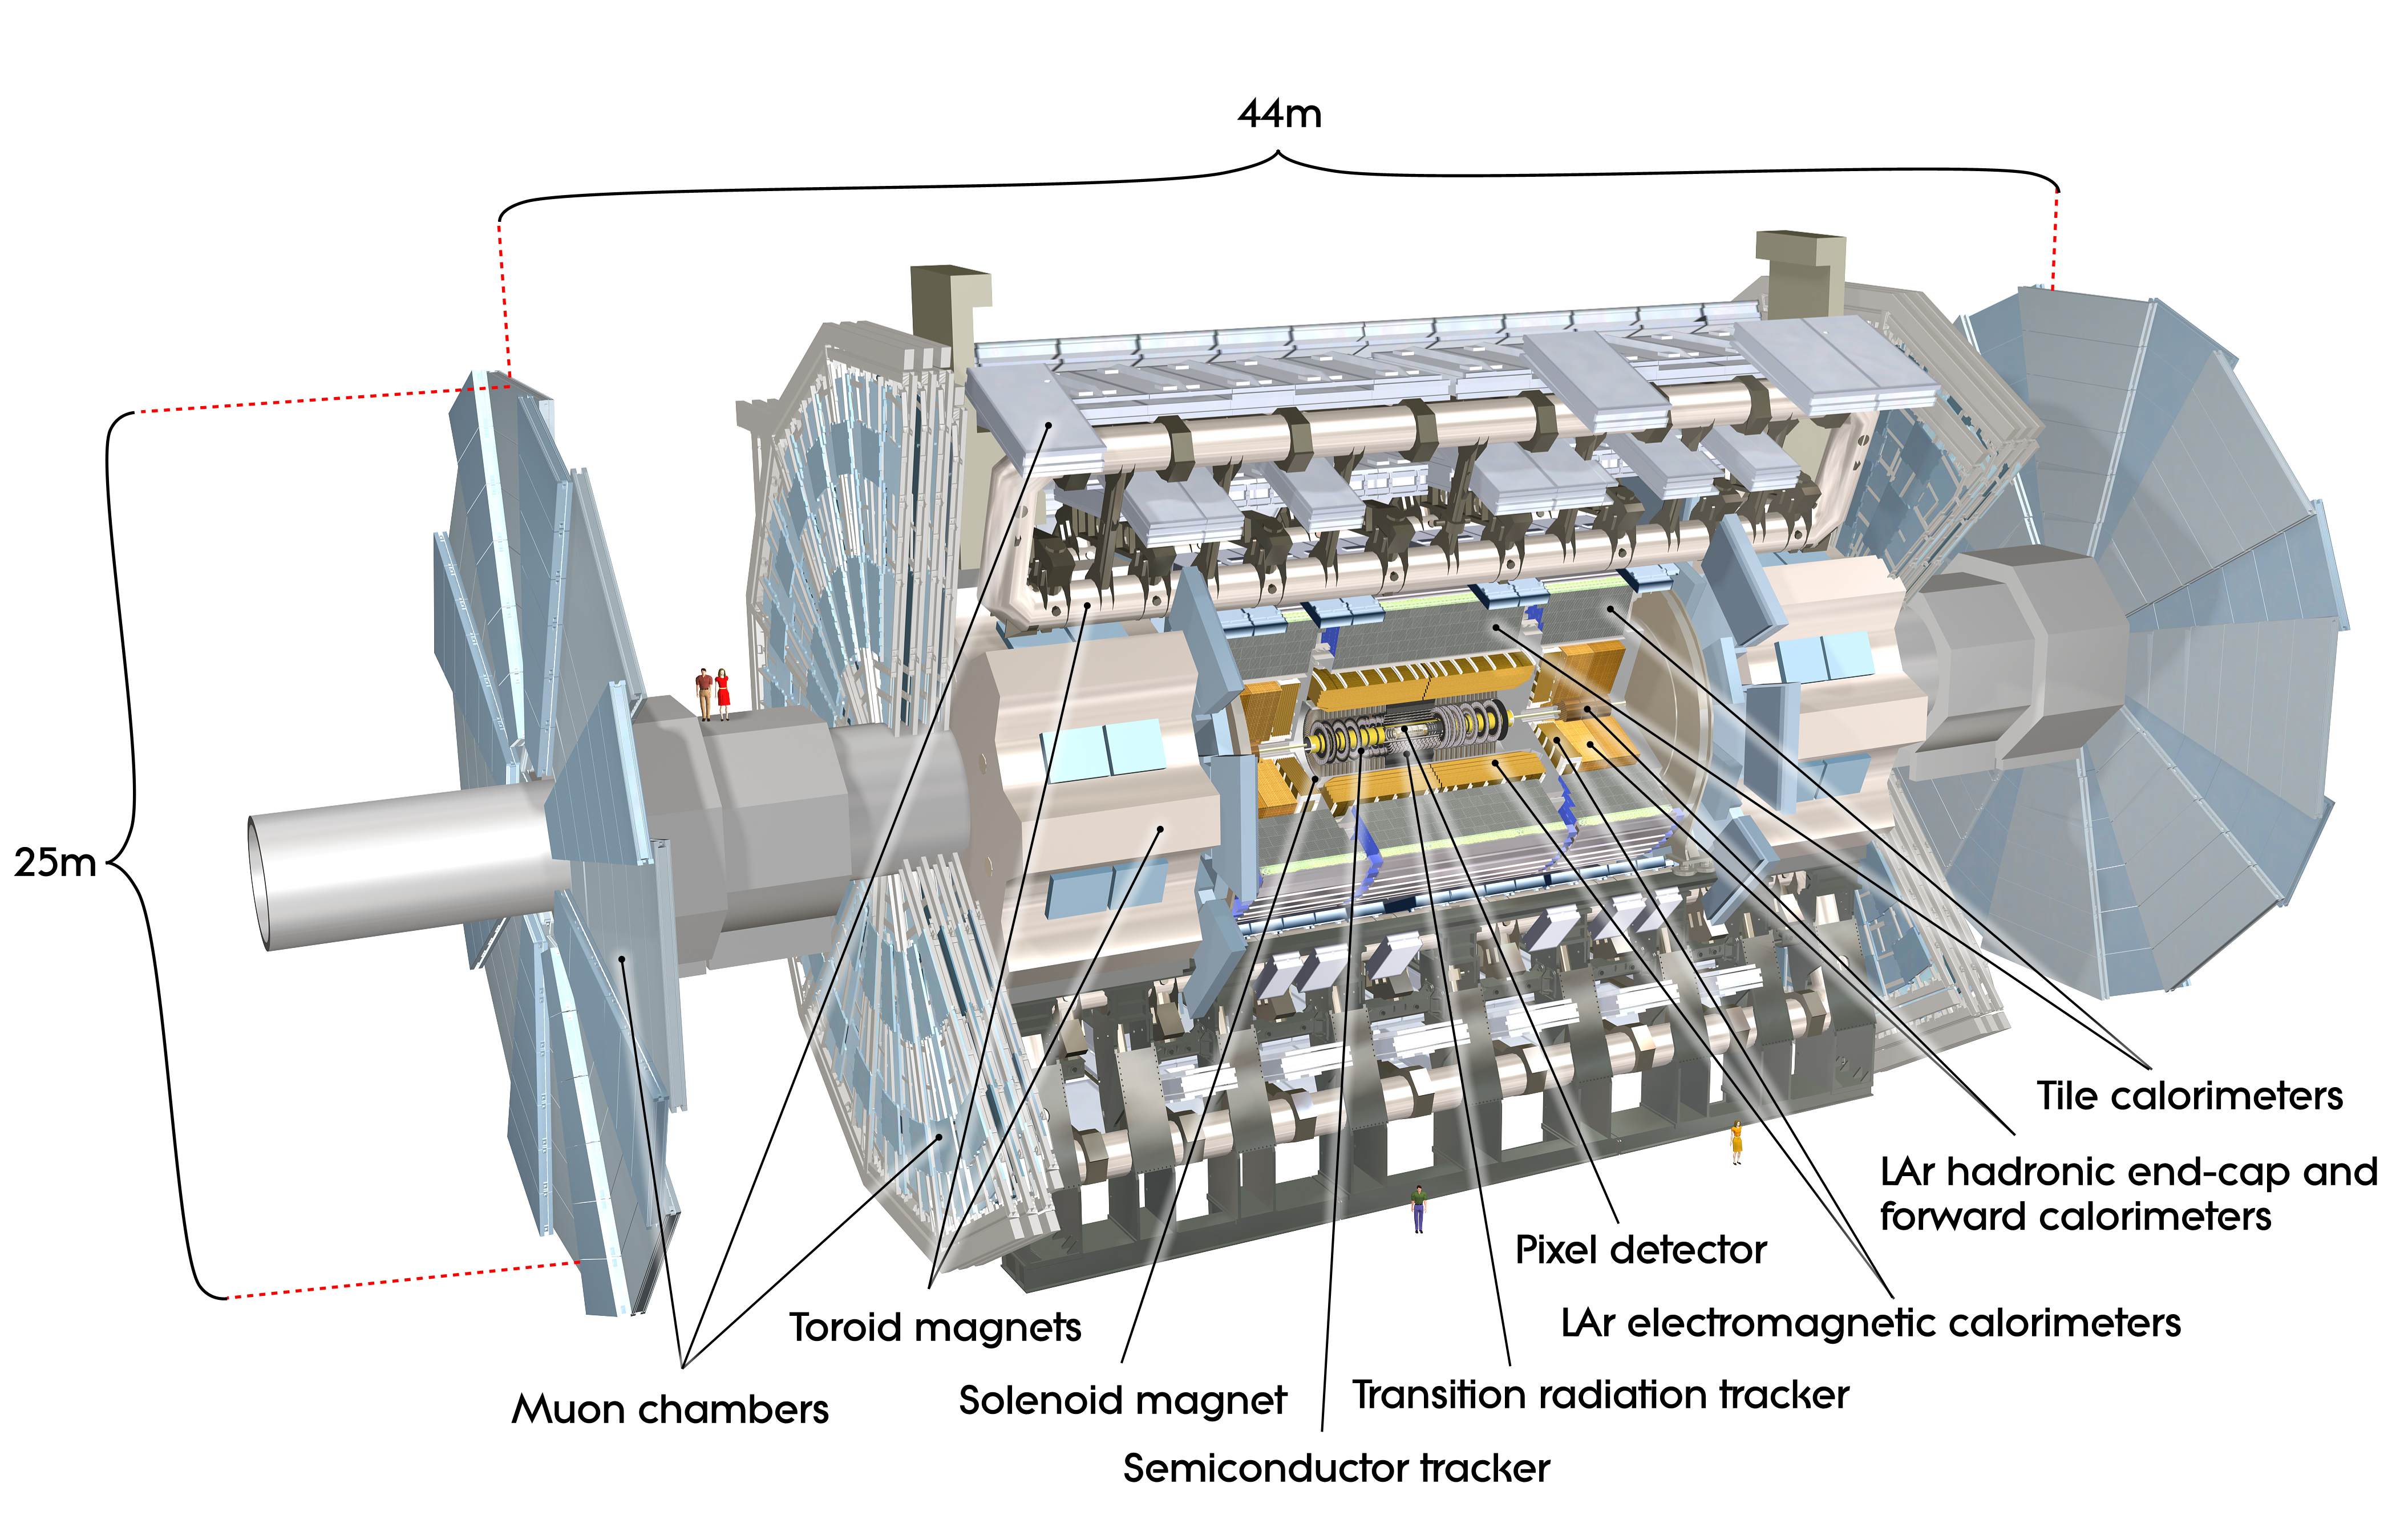
\includegraphics[width=0.90\textwidth]{fig/atlas/atlaspic.jpg}
  \caption{Computer generated illustration of the whole ATLAS detector detector, with various subdetectors highlighted\cite{Pequenao:1095924}.}
  \label{fig:atlas-cgi}
\end{figure}
In order to detect a wide range of physics processes in proton-proton collisions, ATLAS must measure the trajectory and energy of many different kinds of particles, including electron, muons, photons, pions, kaons, protons and neutrons. Once these stable final-state particles are detected, information about the heavier, unstable particles can be inferred. This process is called \emph{reconstruction} and is discussed in detail in Chapter~\ref{ch:objects}.

ATLAS consists of specialized subdetectors designed to capture different phenomena. These subdetectors are arranged as increasingly larger concentric cylinders around the interaction point (IP) where the LHC proton beams collide. There are three main specialized sub-systems: the \emph{inner detector} (ID), which is located just outside the beamline and uses silicon and transition radiation systems to track the trajectory of charged particles; the \emph{calorimeters}, which are located radially outward from the ID and designed to measure the energy of particles with a shower sampling method; and the \emph{muon system}, which is located farthest from the IP and measures muon momentum and trajectory. Details of the subdetectors are provided below. An overview of interaction of different types of particles with the subdetectors as they travel through the detector is illustrated in Figure~\ref{fig:atlas-wedge}.
\begin{figure}[tp]
  \centering
  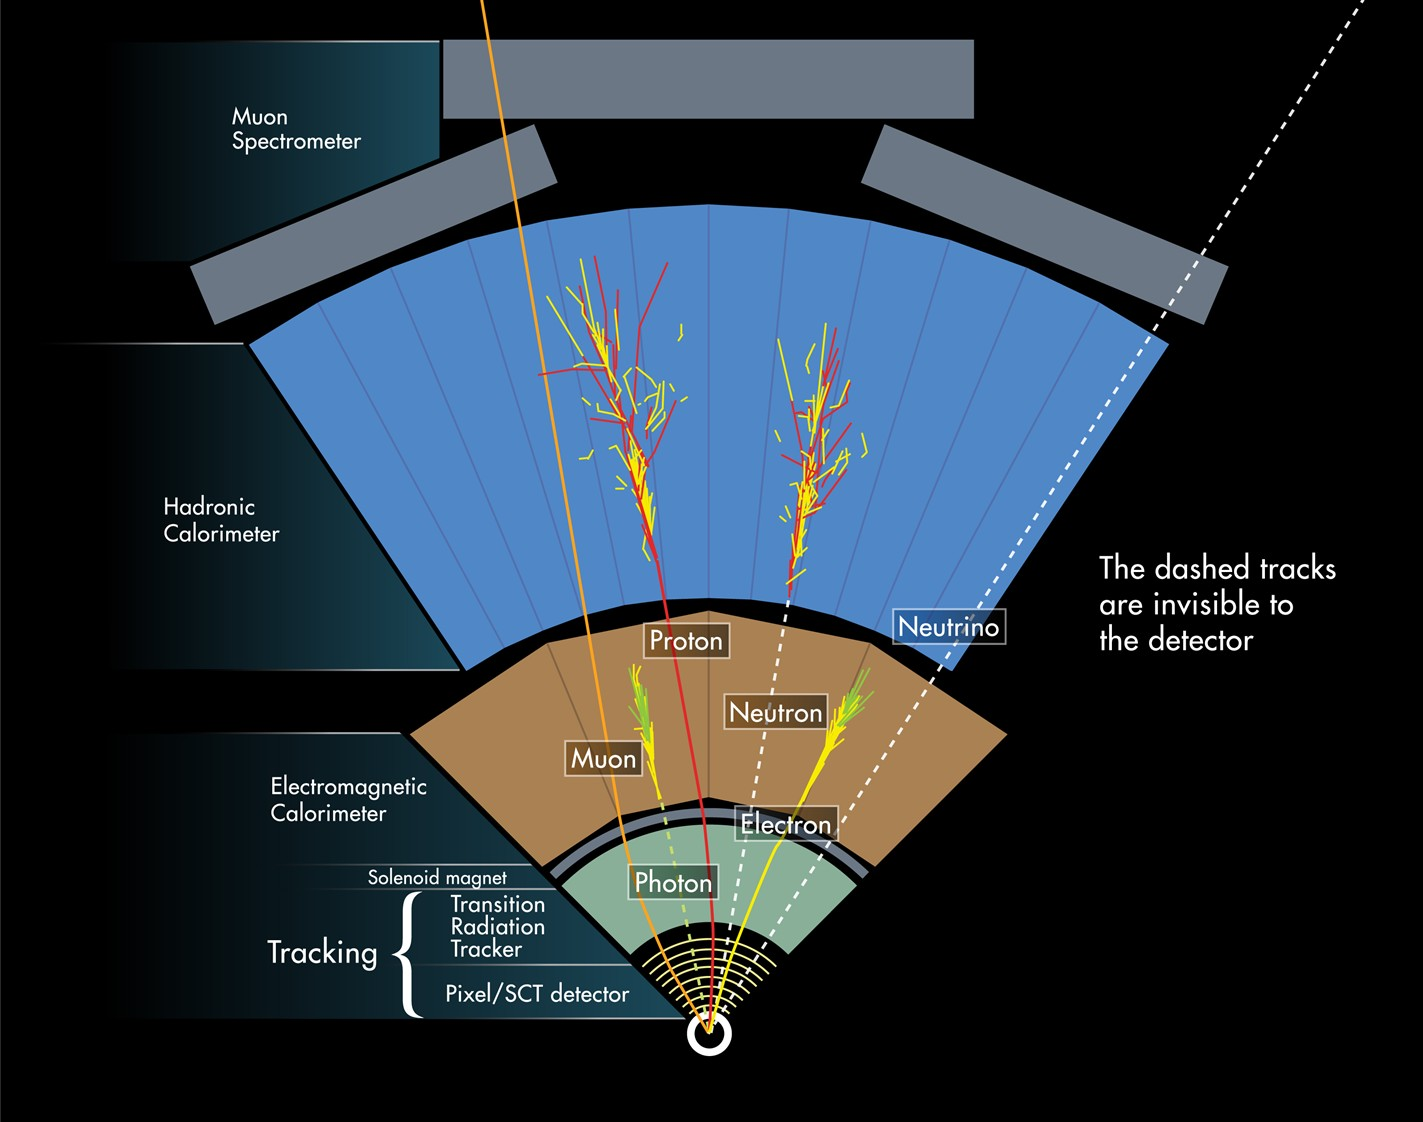
\includegraphics[width=0.90\textwidth]{fig/atlas/atlas-wedge.jpg}
  \caption{A computer-generated image representing how the ATLAS detector functions. The transverse paths of different types of particles are shown interacting with different elements of the detector\cite{atlas-wedge}.}
  \label{fig:atlas-wedge}
\end{figure}

ATLAS has a magnet system that bends the trajectory of charged particles as they travel through the detector. This allows the particles' momenta to be precisely calculated using the classical Lorentz force equation. The magnet system consists of a double configuration. Just outside the ID is a solenoid magnet that produces a field of approximately 2 Tesla. A large toroidal magnet within the outermost part of the detector produces a 1 to 2 Tesla field.


\subsection{Coordinate system}


ATLAS uses a right-handed coordinate system with its origin at the IP in the center of the detector, which is illustrated in Figure~\ref{fig:atlas-coord}. The $z$-axis along the beamline with the positive direction counter-clockwise around the LHC. The $x-y$ plane is defined such that the coordinate system is right-handed, with the $x$-axis pointing from the IP to the center of the LHC, and the $y$-axis pointing upwards. This plane is usually referred to as the transverse plane, since it is perpendicular to the beamline. Cylindrical coordinates, $r$ and $\phi$, are used in the transverse plane with $\phi$ defined as the azimuthal angle around the beamline. Instead of the polar angle from the beamline, $\theta$, pseudorapidity is typically used and is defined as:
\begin{equation}
\eta = -\text{ln}(\text{tan}\frac{\theta}{2})
\label{eq:eta}
\end{equation}
The pseudorapidity is used because in the limit of a massless particle, it is invariant with respect to Lorentz boosts along the beamline. The solid angle distances $\Delta R$ can be measured using the difference in pseudorapidity and azimuthal angle:
\begin{equation}
\Delta R = \sqrt{\Delta \phi^2 + \Delta \eta^2}
\label{eq:dR}
\end{equation}


\begin{figure}[tp]
  \centering
  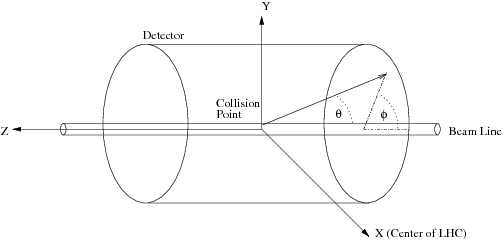
\includegraphics[width=0.90\textwidth]{fig/atlas/coord}
  \caption{Illustration of the ATLAS coordinate system\cite{Schott:2014sea}.}
  \label{fig:atlas-coord}
\end{figure}

% \subsection{Magnets}


%  The solenoid magnet is placed inside the electromagnetic (EM) calorimeter. This is different from most other detector designs where the magnet is placed outside the EM calorimeter. The advantage of the small solenoid is a compact design. A small magnetic field in the EM calorimeter also reduces the transverse spread of showers. The major problem is the increased amount of material in front of the calorimeter which causes many particles to start showering before they reach the active part of the calorimeter.
% The solenoid is a superconducting magnet kept at 4.5 K. To reduce the material the magnet does not have a separate cryostat but rather it shares the cryostat with the liquid argon calorimeter thus saving two cryostat walls. The half length of 2.65 m is considerably shorter than the inner tracking detector. This is a result of a compromise: a short coil reduces the material in front of the calorimeter; a long coil makes the magnetic field more uniform in the Inner Detector. The magnetic field along the z-direction drops from 2 T at the interaction point to around 0.5 T at the end of the Inner Detector.

% The toroid magnet system is divided into one barrel part and two forward systems. With a toroid field, particles will across the complete pseudorapidity range, be almost perpendicular to the field. This means that the field integral  $\int$Bdl , which is the important factor for momentum resolution, can be kept high even in the forward direction. The structure is open with 8 coils in the central region each in separate cryostats. One of the rectangular shaped cryostats can be seen in the front of fig. 4.1. In the forward direction the toroid field is also formed by 8 superconducting coils but there placed in a common cryostat.

% The low number of coils to form the toroid field results in a field strength that varies strongly with the  $\phi$ coordinate. The field integral varies in the barrel from 2-6 Tm and in the end-caps from 4-8 Tm. This is not ideal but an economical necessity.





\section{Inner detector}
The ID is a series of detectors that function as a tracking system to measure the momenta and trajectory of charged particles~\cite{cern-jinst-atlas}. This also allows reconstruction of the primary and secondary vertices of the collision. The innermost part of the entire detector is the pixel detector, 3 layers of silicon that accurately measure the three-dimensional spatial position of charged particles. Next is the SemiConductor Tracker (SCT), 4 layers of double-sided silicon strip modules which accurately measure tracks in the $r-\phi$ plane and are double sided to provide stereo information along the $z$ axis. The outermost component of the ID is the Transition Radiation Tracker (TRT), straw tubes filled with Xenon gas interleaved with polymer layers which provides additional trajectory measurement and differentiate between electron and hadrons. Figure~\ref{fig:id-scheme} shows a schematic outline of the entire inner detector, and Figure~\ref{fig:id-barrel} illustrates a cut-away view of the inner detector barrel.

\begin{figure}[tp]
  \centering
  \includegraphics[width=0.7\textwidth]{fig/atlas/id-schem}
  \caption{Schematic view of the Inner Detector: an $r-z$ slice of the cylindrical barrel, disc endcaps with support tubes, and the solenoid magnet. Lines of constant $\eta$ are drawn~\cite{cern-jinst-atlas}.}
  \label{fig:id-scheme}
\end{figure}
\begin{figure}[tp]
  \centering
  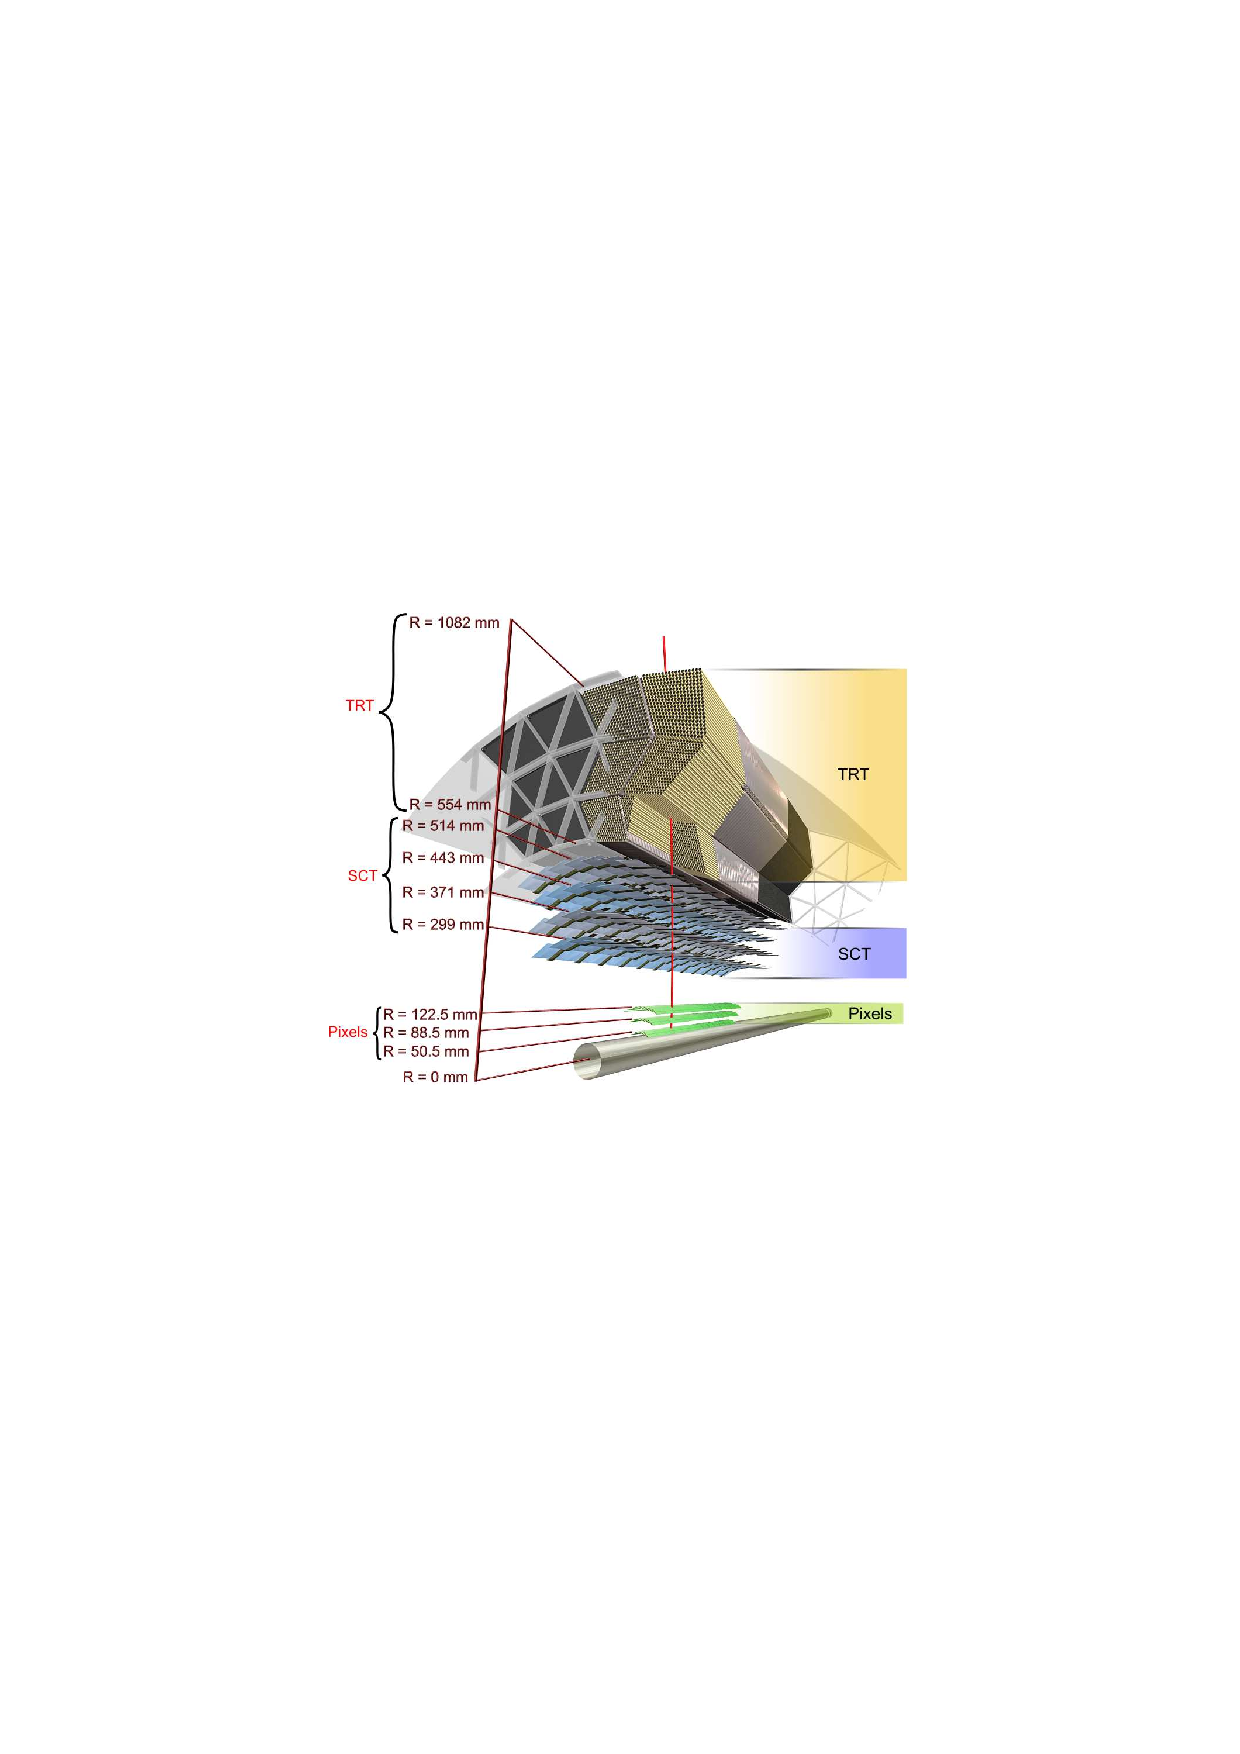
\includegraphics[width=0.7\textwidth]{fig/atlas/id-barrel}
  \caption{A diagram of the barrel of the Inner Detector: the three layers in the Pixels, the four layers in the SCT, and the many layers of the TRT~\cite{cern-jinst-atlas}.}
  \label{fig:id-barrel}
\end{figure}
\subsection{Pixel detector}
The pixel detector is located closest to the beamline and is designed to provide fine granularity in a high radiation environment. Measuring trajectories closest to the interaction point is important for constructing the secondary vertex, necessary for the $b$-tagging of jets used in this analysis.

The pixel detector has 3 barrel layers and three endcap disks on each side of the barrel. The barrel layers are located 50.5 mm, 88.5 mm and 122.5 mm radially from the interaction point. The endcaps sit at 495 mm, 580 mm and 650 mm away from the interaction point. Together, they provide coverage up to $|\eta|=2.5$.

Each silicon pixel in these layers is a p-n junction built of n-type bulk with both p$^+$ and n$^+$ impurities. The additional n$^+$ implants allow the pixels to operate even after the inversion of the bulk from n-type to p-type caused by the high radiation dose. The size of each pixel is $50 \times 400 \micron^2$ with the longer side along the $z$ direction. This allows charged particle hit resolution of approximately 115 $\mu$m in the direction of the $z$ axis and 10$\mu$m in the direction of the transverse plane.

Pixels are bump-bonded to front-end readout chips, with a grid of 2880 pixels connected to each chip. Front-end chips are grouped into rectangular \emph{modules} of dimension $19 \times 63 \micron^2$. Modules in the barrel layers are arranged into long structures parallel to the beamline called \emph{staves}. Staves are tiled at $20^{\circ}$ with respect to the radial direction and overlapped to provide full azimuthal coverage. Endcap modules are arranged into petals and then into wheels, with the sensing element perpendicular to the beam axis. These supporting structures also host power, clock, command and data lines to and from each module. Full coverage is ensured in the endcaps by alternating the placement of the sensors on the front and back of the wheel. The arrangement of the barrel and endcap layers ensures that charged particles with $|\eta|<2.5$ will pass through at least three pixels.

\subsection{SemiConductor Tracker}
The SCT surrounds the Pixel detector and also employs silicon detector elements, using micro-strips instead of pixels. The strips are arranged in four double layers, with the pairs arranged at small angles relative to each other, to make a three-dimensional measurement. The SCT has 4 barrel layers and 2 endcaps, each with 9 disks. 

The SCT is made of single-sided p-in-n sensors of thickness $285\ \micron$ with readout strips. In the rectangular barrel sensors, the readout channels are arrange with a pitch of $80\ \micron$ between them, and the trapezoidal endcap sensors have radial strips with a mean pitch of  $80\ \micron$.  Modules are comprised of four sensors arranged in two layers aligned at a stereo angle of 40 mrad with respect to each other. This allows a single module to measure all three dimensions spatial position of a charged particle passing through both the front and back layers. The endcap wheels are arranged so that charged particles with $|\eta|<2.5$ will pass through at least eight sensors. The 2112 modules in the barrel have resolution a $17\ \micron$ of in $r-\phi$ and $580\ \micron$ in $z$, and the 1976 endcap modules have a resolution of $17\ \micron$ in $r-\phi$ and $580\ \micron$ in $r$.

\subsection{Transition Radiation Tracker}
The outermost layer of the ID is the Transition Radiation Tracker (TRT). The TRT extends the tracking volume to 1106 mm and also distinguishes between electrons and pions based on their transition radiation as they pass through. It consists of straw drift tubes 4 mm in diameter filled with a Xenon gas mixture. At the center of each tube is a 35 $\micron$ diameter anode tungsten wire held at ground potential. Charged particles ionize the gas inside the tube, then the electric field between the tube and the wire creates an ionization cascade, which can be used to infer the energy of the original particle.

The 351,000 tubes are arranged in a barrel and two endcaps. In the barrel, 73 layers of 144 cm long tubes are parallel to the beamline, with wires slit in half to allow separate measurements for positive and negative $z$. In the endcaps, the 160 layers of 37 cm long tubes are arranged radially.  The intrinsic resolution of the TRT in the barrel is $130\ \micron$ in $r\phi$ with coverage up to $|\eta|<2.0$. A changed particle passes usually passes through 30 or more tubes.

When charged particles pass through a polymer fiber mat sitting between the tubes, transition radiation may be produced. These photons from transition radiation produce an ionization cascade much higher than the signal for tracking minimum-ionizing particles. Therefore, TRT straws have two signal thresholds: a \emph{high threshold} for transition radiation hits and a \emph{low threshold} for tracking hits. 

Transition radiation, produced when a charged particle crosses the boundary between two media of different dielectric constants, is proportional to the Lorentz $\gamma$ of a particle. For an electron and charged pion of equal momentum, the electron is about 3.7 times more likely to produce transition radiation than the pion since its mass is 200 times smaller. Seven to ten high threshold hits are typical when an electron passes through the TRT. 



\section{Calorimeters}
The calorimeter system  stops and measures the energy of electrons, photons and jets with full coverage in $\phi$ and $|\eta|<4.9$. This is done with separate electromagnetic and hadronic calorimeters, both with barrel and endcap components. A forward calorimeter provides high $\eta$ measurements. ATLAS calorimeters are sampling calorimeters, which means that only part of the shower energy is observed. Absorbing material used to initiate showers is interleaved with active material for detecting the showers. The layout of the calorimeters can be seen in Figure~\ref{fig:calo}. 

\begin{figure}[tp]
  \centering
  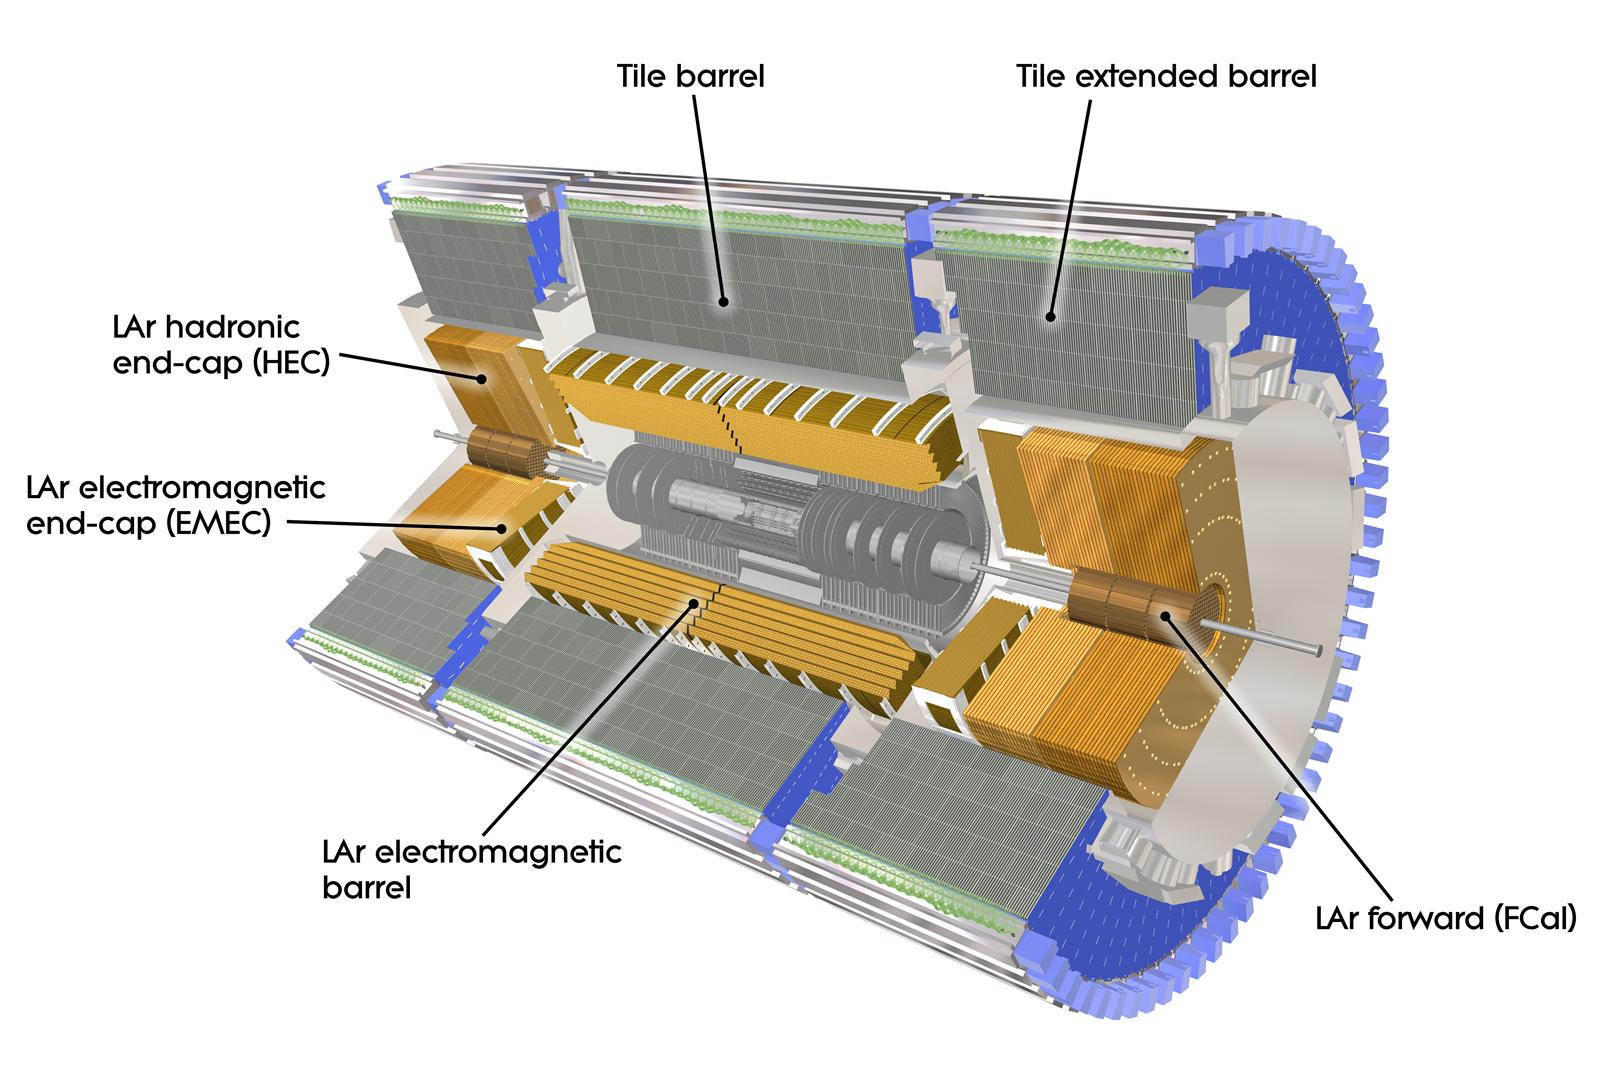
\includegraphics[width=0.95\textwidth]{fig/atlas/combinedCalo}
  \caption{Cut-away view of the ATLAS calorimeter system~\cite{cern-jinst-atlas}.}
  \label{fig:calo}
\end{figure}
\subsection{Electromagnetic calorimeter}
The EM calorimeter has alternating lead absorbers and liquid argon (LAr) active medium with kapton electrodes. The barrel component covers $|\eta| < 1.5$ and the endcap component cover $1.4 < |\eta| < 3.2$. A presampler layer covering $|\eta| < 1.8$ measures showers starting before the calorimeter. 

The barrel is segmented into three layers of decreasing segmentation. The first and second layers are important for identifying shower shapes, so they are finely segmented. The first layer has a thickness of 4.3 $X_0$, and the second layer has a depth of 16 $X_0$, which usually contains the majority of the energy of the EM shower. The third layer is a shallow 2 $X_0$ to capture any leftover energy after the first two layers. To provide prevent gaps in $\phi$, the layers are bent into an accordion-like shape. A diagram of a barrel module is shown in Figure~\ref{fig:caloModule}. The endcap of the EM calorimeter goes out to $|\eta|<$ 3.2 and also has two layers, with an accordion shape oriented such that gaps in $\eta$ are prevented.




\begin{figure}[h]
\begin{minipage}[b]{0.48\textwidth}
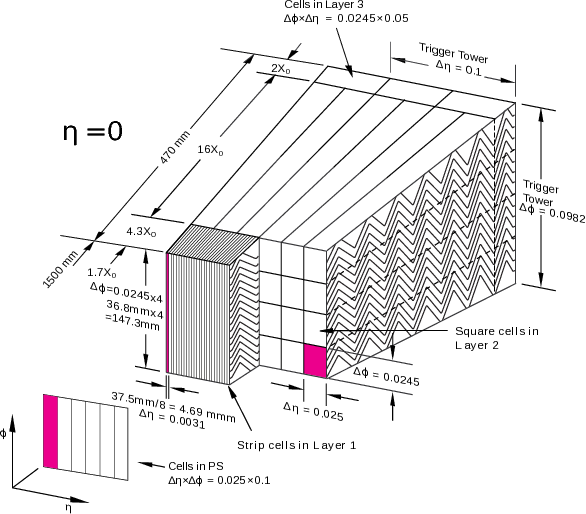
\includegraphics[width=\textwidth]{fig/atlas/caloModule.png}
\caption{Diagram of an electromagnetic calorimeter barrel module\cite{cern-jinst-atlas}.}
\label{fig:caloModule}
\end{minipage}
\hfill
\begin{minipage}[b]{0.48\textwidth}
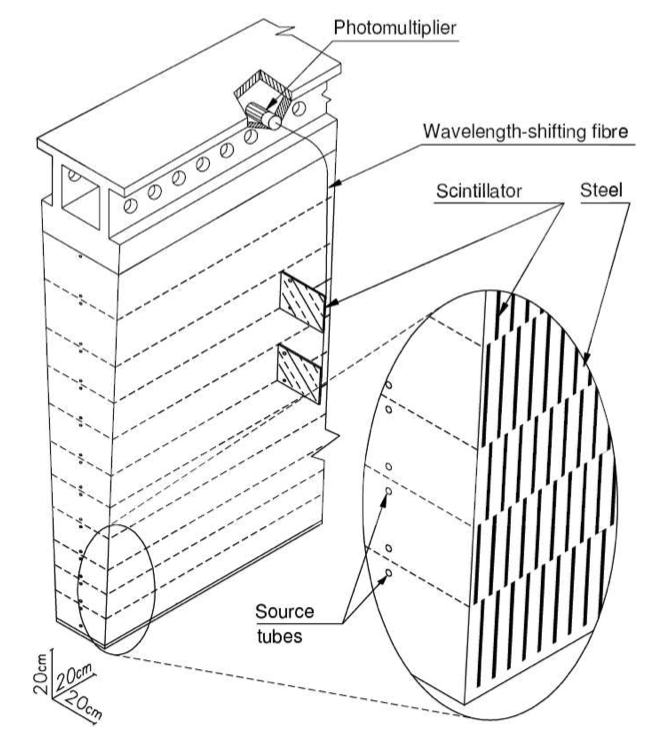
\includegraphics[width=\textwidth]{fig/atlas/tile.png}
\caption{Diagram of a hadronic tile module\cite{cern-jinst-atlas}.}
\label{fig:tileModule}
\end{minipage}
\end{figure}
\subsection{Hadronic calorimeter}
The hadronic calorimeter is divided into three components: the barrel tile calorimeter, which uses steel absorbers and scintillator tiles and covers $|\eta| <$1.7; the Hadronic Endcap Calorimeter (HEC), which uses copper absorber and LAr active material and covers $|\eta|$<3.2; and the forward calorimeter (FCal), which uses LAr active materials and covers $3.1 < |\eta| < 4.9$. The hadronic calorimeters are much coarser than the EM calorimeters because electrons and photons usually don't reach the radius of the hadronic calorimeters, so particle identification isn't a priority. Figure~\ref{fig:tileModule} shows a schematic of a hadronic tile module.
\subsection{Clustering}
\label{ss:cluster}
In order to identify particles, information from the shape of the calorimeter showers must be used. EM particles like photons and electrons produce narrow showers which are largely contained in the EM calorimeters. Hadrons produce broader showers and tend to travel farther into the hadronic calorimeters. Hadronic showers can also contain EM deposits from decays before the calorimeters, such as a neutral pion becoming two photons. In order to turn energy deposits in cells into clusters, information from all of the calorimeters is used as inputs to one of two principal algorithms\cite{ATL-LARG-PUB-2008-002}. The \emph{sliding-window} algorithm clusters cells within fixed-sized rectangles. This algorithm is generally used for electron, photon and tau identification. 

The second algorithm is the \emph{topological} algorithm, which clusters together neighboring cells on the condition that the energy deposit in the cell is significantly more than the expected noise. This algorithm is generally used for jet and missing transverse energy reconstruction. The clusters that result from this algorithm are called \emph{topoclusters.}


\section{Muon System}
The Muon System (MS) is the outermost subdetector, since muons are the only charged particles that can pass though the calorimeters~\cite{2010.muonspectrometer}. The MS consists of a toroidal magnet system and a charged particle tracking system. The components of the muon system, highlighted in Figure~\ref{fig:muonOverview}, are designed to measure the path and energy of muons, particularly high \pt\ muons which may indicate the presence of interesting physics.

The magnetic field provides the bending necessary for charge and momentum measurements and is comprised of three large air-core toroids. The toroid system has eight coils symmetrically around the beam and provides a magnetic field between 2 and 8 Tesla. 

There are two types of tracking systems in the MS. The Monitored Drift Tubes (MDTs) precisely measure the track in the bending direction of the magnetic field and cover $|\eta|<2.7$ in the outer barrel and cover $|\eta|<2.0$ in the inner barrel.  The MDTs are pressurized aluminum drift tubes filled with a mixture of argon and carbon dioxide gas, 30 mm in diameter. Each chamber has 3-8 layer of tubes and a resolution of 35 $\mu$m per chamber. The MDTs are limited to a counting rate of 150 Hz/cm$^2$ and thus cannot be used in the forward region of the inner layer, where high muon rates are expected. This region instead uses Cathode Strip Chambers (CSCs) for momentum measurement with better timing and spatial resolution. The CSCs cover the forward region of the inner layer, 2.0$<|\eta|<$2.7. Two endcap wheels each have 16 chambers. Each chamber has 4 CSC planes. Each plane consists of two cathode strip planes sandwiching anodes wire. The arrangement of the CSCs gives resolution of 40 $\mu$m radial direction and 7 ns timing resolution.

The MS also has two types of trigger chambers: Resistive Plate Chambers (RPC) in the barrel and Thin Gap Chambers (TGC) in the endcaps. Just as with tracking, the endcap and barrel have different types of triggers due to the different rate and precision requirements. The barrel trigger system has 3 RPC layers, and the endcap trigger system has 4 TGC layers. 

\begin{figure}[tp]
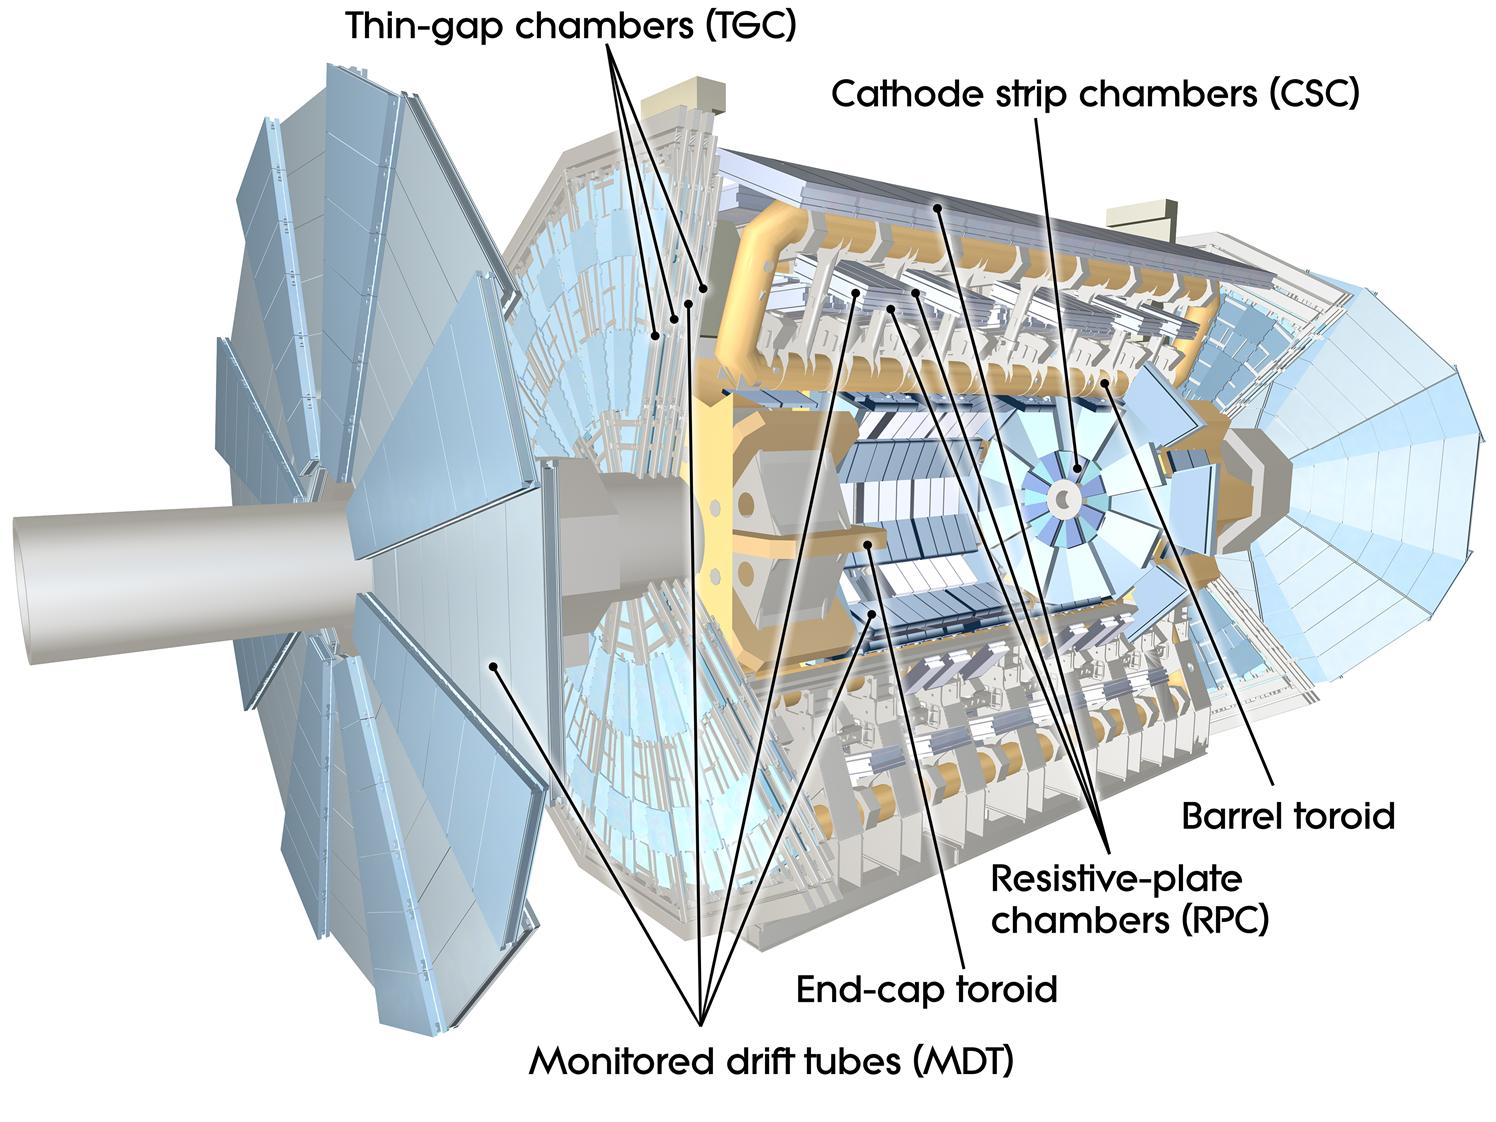
\includegraphics[width=0.95\textwidth]{fig/atlas/muonchamb.jpg}
\caption{Diagram of the muon system\cite{cern-jinst-atlas}.}
\label{fig:muonOverview}
\end{figure}


\section{The trigger system}
At hadron colliders, only a very small fraction of the proton-proton collisions can be feasibly recorded. The majority of events are low energy jets and events that can be used for new physics searches or precision measurements like the Higgs are rarer. With bunch crossings every 50 ns, recording and reconstructing all of the collisions would take an unreasonable amount of data storage and computing power. It would also be impossible to write out events at this rate. Therefore, it is necessary to determine whether a collision will be recorded immediately after it occurs with minimal analysis. 

The process quickly filtering events to record only those of physics interest is called \emph{triggering.} Processes which take place in the trigger system are referred to as \emph{online}. Processes which take place after triggering, such as particle reconstruction, are called \emph{offline}.

The ATLAS trigger scheme\cite{TDR-L1} consists of three stages: Level 1 (L1), Level 2 (L2), and Event Filter (EF). All collision candidates are first run through L1, an online hardware trigger that has coarse granularity by necessity. If events pass the L1 trigger, they are then passed through the offline software triggers, collectively called the High Level Trigger (HLT) and divided into two stages: L2 and EF.

Applying multiplicity and energy threshold requirements, L1 reduces the rate of events from 20 MHz (all $pp$ collisions) to 75 kHz. The L1 trigger only looks at output from the calorimeters and muon system because the inner detector cannot process events at the rate required. In order to process events with the necessary speed, granularity in the calorimeter must be reduced and in the muon system, only the trigger chambers are read out. This reduction in granularity is illustrated in Figure~\ref{fig:l1}. The maximum latency time to process at this level is 2.5 $\mu$s. The data-acquisition system must keep track of which data correspond to which bunch crossing. This presents a substantial challenge since the time for measuring a signal shape in the EM calorimeter is $>100$ ns and the time of flight through the MS is $>25$ ns, both longer than the time between events. 

If the event passes the L1 trigger, then the L2 trigger looks at the distribution of energy deposits as Regions Of Interest (ROIs) identified by L1. The detector signals are compared to a menu of pre-programmed signatures that represent a potential physics object. For instance, a track and a cluster in the EM calorimeter might signal an electron. The L2 looks for these signatures in the ROIs by pulling information from all needed detectors. 

For events with signatures that pass the L2 trigger, all information for the event is read out and the standard offline reconstruction algorithm is run. The event can then be evaluated in terms of the fully reconstructed physics objects to see if particle identities and kinmatics match a menu of desired signatures. Finally, a decision about whether to record the event or not is made. This last stage of the triggering is called the Event Filter. The EF takes about 4s to process each event and can accept events at a rate up to 200 Hz.


\begin{figure}[tp]
  \centering
  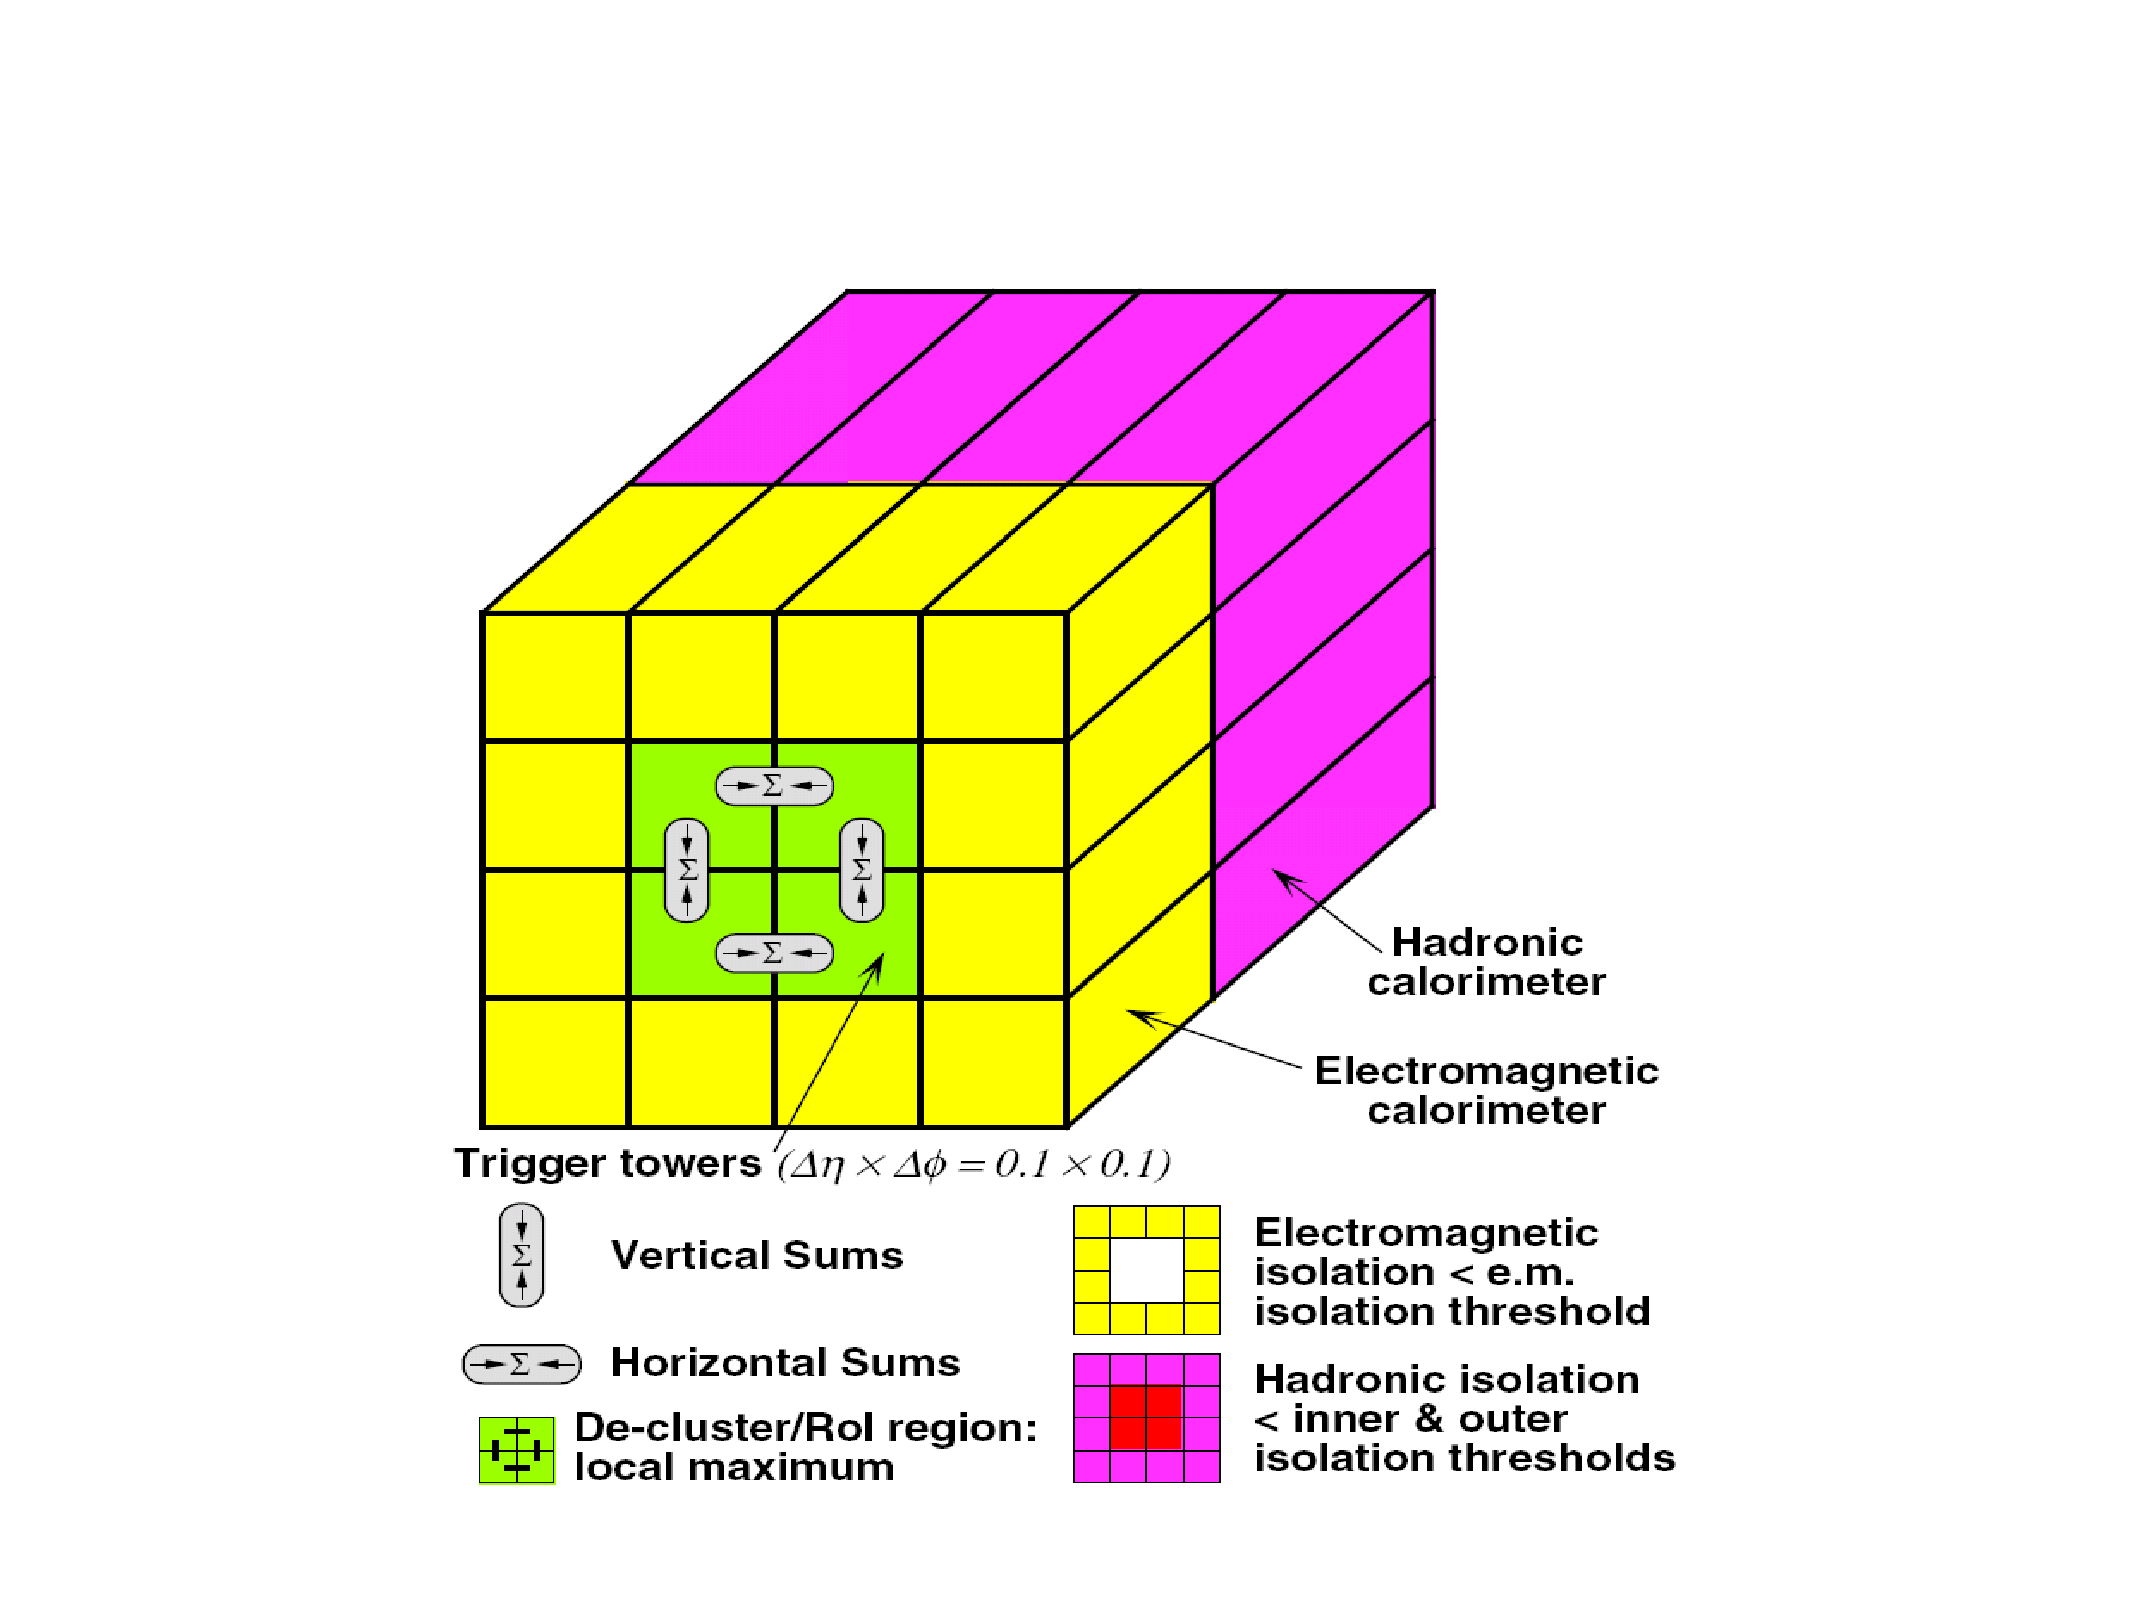
\includegraphics[width=0.80\textwidth]{fig/atlas/cartoonL1.pdf}
  \caption{Schematic view of the calorimeter granularity available at the L1 trigger~\cite{TDR-L1}.}
  \label{fig:l1}
\end{figure}
\subsection{Single electron trigger}
The single electron trigger for used for 2012 is fully described in~\cite{eltrig}. At L1, calorimeters are split into $0.1\times0.1$ towers and then $2\times 2$ clusters are identify $e/\gamma$ leptons using the sliding window algorithm described in Section~\ref{ss:cluster}. Regions of $4\times 4$ with clusters that meet isolation requirements are passed to the L2 trigger as ROIs. At L2, the position of the cluster is identified as the energy-weighted average of the cluster. Track reconstruction is then performed and if a track can be matched to the cluster, it is considered to come from an electron, not a photon. At both L2 and EF, electron candidates are require to pass selection criteria based on the calorimeter cluster and the track, such as cuts on the lateral width of the shower and hits in the inner pixel detector.

In this analysis, the logical OR of two triggers is used to identify electrons: a 24 GeV trigger with a loose track-based isolation requirement and a 60 GeV trigger without an isolation requirement. The isolation requirement specifies that the sum of the \pt of tracks within a cone of $\Delta R$=0.2 must be less than 10\% the \pt of the electron. These trigger chains have thresholds that are maximally efficient for leptons passing offlines selections of $\pT > 25 \GeV$.

\subsection{Single muon trigger}

The single muon trigger for used for 2012 is fully described in~\cite{mutrig}. The muon trigger uses data from the RPCs in the barrel region and the TGCs in the outer region. At L1, the paths between hits in the trigger chambers are interpolated to identify muon candidates. If a hit pattern matches the requirements of the L1 trigger, the $\eta$ and $\phi$ coordinates are passed to the L2 trigger as a ROI. At L2, the MDT and CSC information for the ROI are used to fit a higher quality track. Then, the track in the MS is combined with a track from the ID. Calorimeter data can be used to apply isolation requirements. Quality cuts are applied to the track to determine whether it passes the final trigger chain.

In this analysis, the logical OR of two triggers is used to identify muons: a 24 GeV trigger with a loose track-based isolation requirement and a 36 GeV trigger without an isolation requiment. The isolation requirement specifies that the sum of the \pt of tracks within a cone of $\Delta R$=0.2 must be less than 12\% the \pt of the muon. These trigger chains have thresholds that are maximally efficient for leptons passing offlines selections of $\pT > 25 \GeV$.


\chapter{Analysis strategy}
\label{ch:strategy}
\section{Event selection}
\section{Extra jets}
\section{Correction procedure}
\section{Evaluation of generators}
\chapter{Object reconstruction}
\label{ch:objects}

The analysis relies on the selection of electrons, muons, jets and $b$-tagged jets. This chapter reviews the reconstruction, definition, efficiencies and calibration of these objects in ATLAS.

\section{Object reconstruction}\label{s:objects}
\subsection{Muons}
Muons are reconstructed by combining tracks found in the muon spectrometer and inner detector. Track segments are found in each layer of then detector then combined, taking into account energy loss while crossing the calorimeters. Tracks in the ID are required to pass minimum hit requirements in the Pixel, SCT, and TRT. Muons can be reconstructed using only the MS, but in this analysis uses \emph{combined} muons, reconstructed in both the MS and ID, to ensure high purity.

The muon reconstruction efficiency can be measured using the \emph{tag-and-probe} method. The ID reconstruction efficiency is determined from events reconstructed with one combined muon, the \emph{tag}, and a second muon only required to have an MS track, the \emph{probe}. The ID reconstructrion efficiency is given by the fraction of events where the MS track probe also has a track in the ID. The same method can be used to determine the efficiency of the MS reconstruction as matching. This time, the ID segements are used as the probe and the MS+matching efficiency is given by the fraction of ID segments with a matching MS segment. The overall muon reconstruction efficiency is given by the product of these two efficiencies. To obtain the scale factors (SF), the muon reconstruction efficiency in data and MC is compared: $SF = \epsilon_{data}/\epsilon{MC}$. These scale factors are applied to the simulation to ensure that muons are reconstructed with the same efficiency in MC as in data. For muons, the SFs are calculated in bins of \pt\ and $\eta$ for $Z\rightarrow \mu\mu$ and $J/\Psi\rightarrow \mu\mu$ events~\cite{muonpaper}. 

The muon momentum scale and resolution of the MC must also be corrected to match data. Differences can come from mismodeling of the detector geometry, magnetic field, or energy loss in the calorimeter. Scale factors are determined by comparing the shape of the energy distribution in $Z\rightarrow \mu\mu$ and $J/\Psi\rightarrow \mu\mu$ events. For 2012, the corrections were less than 0.1\%~\cite{muonpaper}.

Finally, the efficiency of the muon trigger is also estimated via the tag-and-probe method. In this analysis, the logical OR of two triggers is used to identify muons: a 24 GeV trigger with a loose track-based isolation requirement (the sum of the \pt of tracks within a cone of $\Delta R$=0.2 must be less than 12\% the \pt of the muon) and a 36 GeV trigger without an isolation requiment. For $\pt<100 \gev$, $Z\rightarrow\mu\mu$ events are used to estimate the trigger efficiency, while $W+$jets is used for \pt\ above this threshold. The muon trigger efficiency in the barrel region is derived from $Z\rightarrow\mu\mu$ events is shown in Figure~\ref{muontrigger}

\begin{figure}[h]
\centering
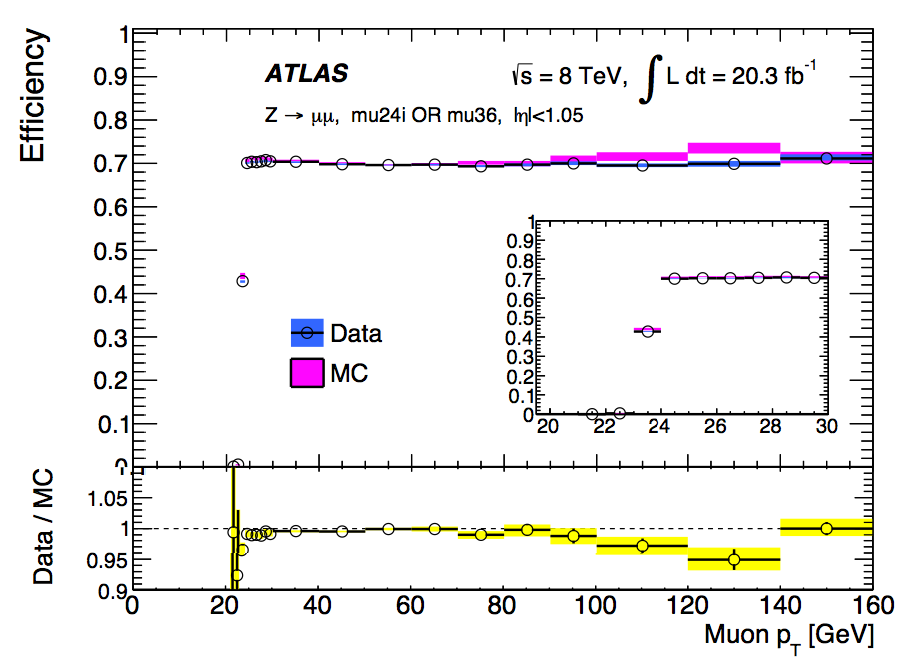
\includegraphics[width=0.6\textwidth]{fig/obj/muontrigger.png}
\caption{Reconstruction and identification efficiency~\cite{Aad:2014fxa}.}
\label{fig:muontrigger}
\end{figure}
\subsection{Electrons}





\chapter{Event selection}
\label{ch:event}
The following section describes the procedure used to select the events used for analysis. First, the data and simulation samples to be used are defined. Then, the fiducial definition of the physics objects used to select the events is given. Then, the criteria for selecting events is discussed. Finally, the event yields and reconstructed distributions are reviewed. 

\section{Data samples}
\subsection{Collision data}
The analysis is performed on the complete 2012 $pp$  \rts=8 \tev\ LHC collision dataset. Events are required to
fulfill standard data quality requirements that ensure that all detector components are functioning. Events are required to pass a single electron or single muon trigger chain, with thresholds that are maximally efficient for leptons passing offline selections of $p_T>25$\,GeV. % For electrons, the OR of the \texttt{ EF\_24vh\_medium1}\ and \texttt{ EF\_e60\_medium1}\ trigger chains is used. For muons, the OR of \texttt{ EF\_mu24i\_tight}\ and \texttt{ EF\_mu36\_tight} is used. In each case, the higher threshold trigger has no isolation requirement, and adds to the acceptance of the lower threshold trigger at higher lepton $p_T$. 

Events are selected from both \texttt{ Egamma} and \texttt{ Muons} data streams defined by the trigger chains. To avoid double counting of $e\mu$ events appearing in both streams, events passing electron triggers are only accepted from the \texttt{Egamma} stream, {\em i.e.} the \texttt{ Muons} stream is only used for events selected \emph{only} by muon triggers. 
After all these selections, the final analyzed data samples correspond to an integrated luminosity of 20.3\,\ifb\ with an uncertainty of 2.8\%.
\subsection{Simulated Samples}

Simulated Monte Carlo event samples are used in this analysis to evaluate the efficiency and uncertainty of signal and background.  Both uncorrected and corrected data distributions are also compared to simulated samples to distiguish between physics models. .% The corresponding dataset (DS) identification numbers are given  in Tables~\ref{t:ttsamples},~\ref{t:bgsamples}, and ~\ref{t:wtsamples} and a complete list of dataset names is provided in Appendix~\ref{app:ds}.

Samples are processed either through the full ATLAS Geant4\cite{bib:g4} based detector simulation (``FS'') or through the \texttt{ AtlFast2}\cite{atlfast2} fast simulation. All samples include additional overlaid minimum bias events generated with \textsc{  Pythia8} \cite{pythia8} to simulate pileup background. 
The simulated samples are reweighted to reproduce the same distributions of $\mu$, the average number of interactions per bunch crossing, as the data. The samples are also reweighted with scale factors to reproduce the electron and muon reconstruction and trigger efficiencies, and the width of the primary vertex distribution in $z$, as measured in the data. Finally, scale factors are applied to account for $b$-tagging efficiencies. 

\subsubsection{\ttbar samples}\label{ss:mcsignal}

Several different \ttbar\ generators are compared to data. The baseline \ttbar\ samples are produced using \textsc{  Powheg} \cite{Powheg, Powheg2, Powheg3, Powheg4} interfaced to \textsc{  Pythia6} \cite{pythia6} with the Perugia 2011C tune \cite{perugia}, CT10 parton density functions (PDFs) \cite{cttenpdf}, the hdamp parameter set to $\infty$ and fast simulation.  
This same MC tune has been processed using full simulation and the results of the two samples have been compared.
%After appropriate
%JES corrections are applied, systematic differences in the prediction are observed. 
%The stress test in Chapter~\ref{sec:unfold} confirms the agreement of these two samples.
The atlfast2 sample with the hdamp parameter set to $\infty$ is chosen as the baseline because it has signifigantly higher statistics ($\sim 40$ times data) than either the FS or hdamp=$m_t$ samples ($\sim 20$ times data).
Systematic uncertainties associated with the difference in the response matrices obtained from FS and atlfast are
assessed in Chapter~\ref{ch:syst}.


%For the baseline dataset, samples using both full and fast  simulation are analyzed to confirm that after making appropriate JES corrections, there are no differences in the predictions.

Alternative \ttbar\ simulation samples are also studied.  At next-to-leading-order, these include \textsc{  Powheg} plus \textsc{  Pythia6}  with the hdamp parameter set to $m_{t}$; \textsc{  Powheg} plus \textsc{  Pythia8} with the hdamp parameter set to $m_{t}$ and the A14 tune ; \textsc{  MC@NLO} \cite{mcatnlo, mcatnlo2} interfaced to \textsc{  Herwig} \cite{Herwig, Herwig1, Herwig2} with \textsc{  Jimmy} \cite{jimmy} for the underlying event modeling and with the ATLAS AUET2 \cite{auet} tune and CT10 PDFs; and \textsc{  Powheg} plus \textsc{  Herwig}. 
Alternate multi-leg leading order samples include \textsc{  MadGraph} \cite{Alwall:2011uj} interfaced to \textsc{  Pythia6} \cite{pythia6} with the Perugia 2011C tune \cite{perugia}, and CT10 parton density functions (PDFs) \cite{cttenpdf}; \textsc{  Alpgen} \cite{alpgen} interfaced to \textsc{  Herwig} and \textsc{  Jimmy}, with
the CTEQ6L1 PDFs \cite{CTEQ}; and \textsc{  Alpgen} interfaced to \textsc{  Pythia6}
. To study the effects of initial and final state radiation (ISR/FSR), several samples with different radition parameters were used.

%ADD IN HERWIG FOR PARTON SHOWERING+MADGRAPH Q2+ISR FSR

The \textsc{ Powheg} and \textsc{ MC@NLO} samples include all \ttbar\ final states except fully-hadronic, where both $W$ bosons decay to \qqbar\ giving a negligible probability to pass the event selection. The \textsc{  MadGraph} sample only included dileptonic final states, where both $W$ bosons decay to leptons. Most of these MC samples contain more than ten times the data statistics.

\subsubsection{Single top samples}
Only the $Wt$ channel of single top production contributes significantly to \emubb\ events. Single top production is modeled using \textsc{  Powheg+Pythia} with the CT10 PDFs and the Perugia P2011C tune, using the `diagram removal' \cite{Frixione:2008yi} generation scheme. Alternative physics models include the \textsc{  Powheg+Pythia} sample with `diagram subtraction' \cite{Frixione:2008yi} and \mcnlohw.

\subsubsection{Background samples}\label{ss:mcbkg}

$Z$+jets events with $Z\rightarrow \ell^-\ell^+$ and diboson production ($WW$, $WZ$ and~$ZZ$) where both bosons decay leptonically can contribute to background. $Z$+jets background is modeled using \textsc{  Alpgen} \cite{Mangano:2002ea} with CTEQ6L1 PDFs, interfaced to \textsc{  Pythia6} with the Perugia P2011C tune, including both samples with 0--5 additional light partons, 
\ccbar\ plus an additional 0--3 partons, and \bbbar\
plus 0--3 partons. The heavy flavor overlap procedure (HFOR) \cite{hfor} is used to avoid double counting of configurations where the \ccbar\ or \bbbar\ pair could be produced from either the matrix element or parton shower. The simulated $Z+$jets  events are scaled by the ratios of $Z\rarrow ee$+2 $b$-jets or $Z\rarrow \mu\mu$+2 $b$-jets measured in simulation and data, to account for the mismodeling of heavy-flavor jets produced with $Z$ bosons. Ref.~\cite{xsec} computes this scale factor to be $1.13 \pm 0.08$. 

Diboson production is simulated using \textsc{  Alpgen+Herwig} with up to three additional partons.

\subsection{Pileup jet samples}
Modeling of pileup collisions (see Chapter~\ref{ch:atlas}) is studied both using the default \powpy\ generator as well as a data driven estimate. The data driven \emph{overlay} sample takes pileup events from data and combines them with \ttbar\ events from \powpy\. The difference between these two estimates is taken as a systematic uncertainty.
\section{Object definitions}
The object and event selection used in this thesis follows the generic ATLAS recommendations for 2012, with two exceptions.  The first change is a loosening of the electron isolation criteria, which is possible due to the low background  $e\mu$ final state. This loosened requirement is also used in Ref.~\cite{xsec}. The second change is to relax the $\eta$ requirement on  jets to $|\eta|<4.5$.

\subsection{Reconstructed objects}\label{s:objects}

The analysis relies on the selection of electrons, muons and jets, and
the tagging of jets as $b$-jets.
\begin{description}
\item[Muons:] Combined muons (reconstructed in both the muon spectrometer
and inner detector) are required to satisfy $p_T>25$\,GeV and $|\eta|<2.5$.  Muons must have
\begin{itemize}
\item at least one pixel hit
\item at least 5 SCT hits
\item fewer than 3 holes in pixel and SCT layers combined
\item In the region $0.1 < |\eta| < 1.9 $: $n_{TRT Hits} + n_{TRT Outliers} > 5$ and $\frac{n_{TRT Hits}}{n_{TRT Hits} + n_{TRT Outliers}} < 0.9$, where an outliter is a TRT straw with a signal but not crossed by the nearby track.
\end{itemize}

The impact parameter
in the longitudinal direction with respect to the primary vertex is
required to satisfy $z_0<2$\,mm.  To reduce the background from
muons from heavy flavor decays inside jets, muons are required to be
separated by $\Delta R>0.4$ from the nearest jet. Muons are required to satisfy 
mini-isolation requirement $I^\ell_{\textrm mini}<0.05$, where
the mini-isolation variable is the ratio of the sum of $p_T$ of tracks
in a variable-sized cone of radius $\Delta R=10\,{\textrm GeV}/p_T(\mu)$ to the $p_T$ of the muon $p_T(\mu)$ \cite{topreco}. %For anti-muons, the mini-isolation requirement is energy loss of less than 6 GeV, $\texttt{ ETCone20}/p_{T} < 0.03$, and $I^\ell_{\textrm mini}<0.1$

\item[Electrons:] Electrons are selected using the offline \texttt{ tight++} 
identification within the fiducial region $p_T>25$\,GeV and $|\eta|<2.47$, 
excluding the calorimeter transition region $1.37<|\eta|<1.52$. The impact parameter
in the longitudinal direction with respect to the primary vertex is
required to satisfy $z_0<2$\,mm. In addition 
to the calorimeter isolation requirements implicit in \texttt{ tight++},
the calorimeter energy in a cone of radius $\Delta R<0.2$ around the
electron (excluding the deposit from the electron itself) is required
to be less than $6$\,GeV, and the sum of $p_T$ of tracks
in a cone of radius $\Delta R<0.3$ (excluding the electron track) is
required to be less than 6 \GeV. Further
kinematic-dependent cuts are applied to these two isolation variables,
corresponding to a 98\,\% efficiency on true prompt electrons. 
\item[Overlap removal:]
To prevent double-counting
of electron energy deposits as jets, jets within $\Delta R<0.2$ of 
a reconstructed electron are removed. If the nearest jet surviving
the above cut is within $\Delta R<0.4$ of the electron, the electron
is discarded, to ensure it is cleanly separated from nearby jet activity. Electrons sharing a track with a muon are excluded by removing electrons with a muon within $\Delta \phi < 0.005$ and $\Delta \theta < 0.005$.

\item[Jets:] Jets are reconstructed using the anti-$k_t$ algorithm 
\cite{antikt1,antikt2,antikt3} with radius parameter $R=0.4$, 
starting from topological clusters. These are calibrated
using the local cluster weighting (LCW) method, and corrected for the
effects of pileup using the jet area method and a residual correction dependent
on the instantaneous luminosity and number of reconstructed primary vertices 
in the event. Jets are calibrated using an energy- and $\eta$-dependent simulation-based calibration scheme, with in-situ corrections 
based on data \cite{jesxi}. Jets are accepted within the fiducial region $p_T>25$\,GeV and $|\eta|<4.5$. To reduce the contribution from jets 
associated with pileup jets with $p_T<50$\,GeV
are required to satisfy $|\textrm{JVF}|>0.5$, where $\textrm{JVF}$ is
the ratio of the sum of the $p_T$ of tracks associated to the jet which
are also associated to the primary vertex, to the sum of $p_T$ of all
tracks associated to the jet. Jets with no associated tracks or with
$|\eta|>2.4$ at the edge of the tracker acceptance  are assigned
$\textrm{JVF}=-1$ by convention and thus always accepted.
Reconstructed jets 
within $\Delta R<0.2$ of a selected electron are removed.

\item[$b$-tagging:] Jets within the central region ($|\eta| < 2.5$) are $b$-tagged using the MV1 algorithm 
\cite{btagcom,btagptrel}, which outputs a multivariate discriminant $w$ with values between zero and one. 
Light-quark and gluon jets tend to have values close to zero, and 
$b$-flavored jets close to one, with charm jets somewhere in between. Jets are defined as being $b$-tagged if the MV1 weight $w$ is larger than a cut value 0.7892, which corresponds to the $b$-tagging working 
point having approximately 70\% $b$-tagging efficiency for $b$-jets in \ttbar\ events, although the exact efficiency varies significantly with $p_T$. The $b$-tagging calibration used is the default in \texttt{ TopRootCore}, which is based on the system8 muon and jet calibration method~\cite{btagsys8}.
\end{description}
Events reconstructed with exactly one $e$ and $\mu$ with opposite sign and at least 2-$b$ jets as defined above pass the reconstruction-level fiducial selection. In the case of Monte Carlo, selected events are reweighted to reproduce the same distributions of $\mu$, the average number of interactions per bunch crossing, as in the data. The samples are also reweighted with scale factors to reproduce the electron and muon reconstruction and trigger efficiencies, and the width of the primary vertex distribution in $z$, as measured in the data. Finally, scale factors are applied to account for $b$-tagging efficiencies.
\subsection{Truth objects}
In addition to fiducial definitions for reconstructed from detector output, fiducial definitions for the ``true'' particles generated by the MC simulation must be made. The cuts applied to truth objects attempt to replicate the above fiducial selections for the reconstructed objects as closely as possible.

\begin{description}
\item[Leptons:] Stable electrons and muons are required not to come from a hadron in the Monte Carlo truth particle record, either directly or through a tau decay. This ensures that the lepton is from an electroweak decay without requiring a direct $W$-boson match. The four momenta of the bare leptons are then `dressed' by adding the four momenta of all stable photons within $\Delta R$=0.1 with status code 1 and not originating from Geant4. The dressed leptons are required to have \pt $>$ 25 \GeV\ and $|\eta|$ $<$ 2.5.
\item[Jets:] Truth jets are clustered using the anti-$k_t$ algorithm  with radius parameter $R=0.4$, starting from all stable particles, except for selected leptons ($e$, $\mu$, $\nu$) and the photons used to dress the leptons. Truth jets are required to have \pT $>$ 10 \GeV, $|\eta| <$ 4.5. Though only jets with \pT $>$ 25 \GeV\ are considered in the final result, lowering the \pt\ requirement for truth jets allows matching across the fiducial boundary. This is discussed in more detail in Chapter~\ref{ch:extrajets}.

\item[$b$-tagging:] $B$ hadrons with \pT $>$ 5 \GeV\ are associated with jets through ghost matching~\cite{ghostmatch}. Truth $b$-tagged jets have \pT $>$ 25 \GeV, $|\eta|$ $<$ 2.5 and at least one ghost associated $B$-hadron with $p^{{\textrm B}}_{T} > 5$ \GeV.

\item[Overlap removal:] Truth objects are subject to the same overlap removal criteria as reconstructed objects, after dressing and jet reclustering. The closest jet within $\Delta R$ $<$ 0.2 of an electron is excluded from consideration.  After such jets are removed, 
muons  and electrons with $\Delta R$ $<$ 0.4 of a jet are excluded. Electrons overlapping with muons are removed if $\Delta \phi_{e\mu} < 0.005$ and $\Delta \theta_{e\mu} < 0.005$.
\end{description}


Events with exactly one $e$ and $\mu$ with opposite sign and at least 2-$b$ jets as defined above pass the fiducial truth selection.

\subsection{Truth matching}

\label{ss:tmatching}
In order to correct reconstructed objects back to truth level, a prescription must be adopted to match reconstructed and truth objects. A geometric $\Delta R$ algorithm matches reconstructed objects to truth objects satisfying the fiducial requirements above. These definitions are relevant for background unmatched extra jets, as well as various truth studies.
\begin{description}
\item[Leptons:] Each truth $e$ ($\mu$) is matched to the closest reconstructed $e$ ($\mu$) within $\Delta R < 0.02$.
\item[Jets:] Truth jets are geometrically matched to the closest reconstructed jet within $\Delta R_{\mathrm{reco jet, truth jet}} < 0.4$. If a reconstructed jet is not matched to a truth jet, it is assumed to be either from pileup or matching inefficiency and is treated as background as discussed in Chapter~\ref{ss:pileup}.

In selecting $e\mu$+2 $b$-jet events, $b$-jets are matched to truth jets before extra jets are matched to truth jets. Thus, if both an extra jet and a $b$-jet satisfy $\Delta R_{\mathrm{reco jet, truth jet}}<0.4$, the $b$-jet is matched to the truth jet and the extra jet is unmatched. If two $b$-jets or two extra jets are reconstructed within $\Delta R_{\mathrm{reco jet, truth jet}}<0.4$ of a single truth jet, the reconstructed jet with smaller $\Delta R_{\mathrm{reco jet, truth jet}}$ is matched to the truth jet and the other reconstructed jet is unmatched.

Because of limited \pt\ resolution, the reconstructed \pt\ of a jet can vary significantly from its truth \pt. The \pt\ threshold for truth jets is lowered to 10 \GeV, so that jets reconstructed with $\pt > 25 \GeV$ can match truth jets that fail the fiducial \pt\ cut. 



\item[Parton matching:] For some studies, the truth jets from top are identified via a parton matching procedure. Each jet is matched to the highest energy parton\footnote{Quarks (u,d,s,c,b), gluons, photons and pdgId = 0 particles.} with \pt $>$ 5 \GeV\ within $\Delta R = 0.4$. If this parton is a decay product of the top, then the jet is considered a `top jet.'
\end{description}
\section{Event selection}
The process of selecting \emubb\ events proceeds as follows. First, events are selected from simulation and data by vetoing a small number of events failing cleaning cuts defined below. Then events are required to have exactly one electron and one muon with opposite charges. Finally, events with at least two $b$-tagged jets are selected. In events with more than two $b$-tagged jets, the two $b$-jets with the highest MV1 are considered the $b$-jets used to select the event and the remaining $b$-jet(s) are considered extra jets. The selection requirements are identical to those in the 2012 \ttbar cross-section analysis~\cite{xsec}, with the exception of requiring \textit{at least} two $b$-tagged jets instead of \textit{exactly} two.

\subsection{Cleaning cuts}

Events are required to have at least one reconstructed primary vertex with at least five associated tracks. Events containing any jets with $p_T>20\GeV$ and positive energy that fail the `Bad Loose Minus' (also known as  `Looser') jet quality cuts \cite{jetcleaning} are removed (`jet cleaning'). To remove events containing cosmic rays, events with two muons passing the muon selection requirements given above, each having an impact parameter with respect to the primary vertex $d_0>0.5$\,mm and separated in azimuthal angle $\phi$ by $\Delta\phi>3.1$\,rad, are vetoed.

A muon undergoing catastrophic bremsstrahlung/energy loss in the calorimeter
can leave a large energy deposit, causing it to be reconstructed as both
an electron and a muon, and potentially giving rise to a fake $e\mu$ event.  Such background is reduced by vetoing $e\mu$ events if the electron and muon are separated by $\Delta\phi<0.005$ and $\Delta\theta<0.005$, where $\phi$ and $\theta$ are the azimuthal and polar angles of the selected leptons
(muon bremsstrahlung cut).

\subsection{Event yields}

The numbers of events with exactly one $e$ and one $\mu$ before and after the $b$-jet requirement are given in Table~\ref{t:sel}. Simulation predictions are categorized into contributions from \ttbar, $Wt$ single top, $Z$+jets and dibosons. 

After the selection of $e\mu$ opposite-sign pairs, the biggest contribution (60\%) is from \ttbar events with the second largest from $Z$+jets (21.8\%). The $e\mu$ event rates agree to  better than 3\% with those from other ongoing 2012 top analyses as documented in \texttt{ TopEventChallenge}\cite{topeventchallenge}. The events with at least 2 $b$-jets are heavily dominated by \ttbar events, with a small $\sim 3\%$ contribution from single top. $Z$+jets and dibosons make up less than 0.1\% of events passing the final selection, and are thus neglected in this analysis.


The number of selected events in simulation and data agree to within better than 3\%, demonstrating that the Monte Carlo reproduces the data quite well. Table~\ref{t:ttgen} compares the number of selected events from the baseline \ttbar simulation to those from other \ttbar generators. The two \pow+\py\ simulations and \mcnlohw\ all agree with each other to within ~2\%. The \madpy\ simulation gives about 10\% more events. The last column in Table~\ref{t:ttgen} gives the scale factor used to normalize each \ttbar generator to the number of events in data (including the single top contribution).

%To facilitate comparison with Ref.~\cite{xsecnote}, Table~\ref{t:exact2sel} gives the number of \ttbar simulation and data events with exactly 2 $b$-jets. Removing events with more than 2 $b$-jets reduces the number of events by ~2\% in both simulation and data. The event counts given in Table 4.2 of Ref.~\cite{xsecnote} are not directly comparable because they exclude contributions from misidentified leptons and correspond to a greater luminosity of 20.3\ifb. Adding back in the misidentified lepton contribution and then scaling by $20.1/20.3=0.989$ gives an `adjusted' event count in the final column. This analysis finds 2.1\% more events in data and 0.3\% more events in simulation than Ref.~\cite{xsecnote}. These differences are likely due to the new calibrations used in this analysis.


\subsection{Reconstructed distributions}
In Figures~\ref{fig:emu} and ~\ref{fig:bjet}, the properties of reconstructed lepton and $b$-jets in $e\mu$+2 $b$-jet events are compared in simulation and data. The negligible contributions from $Z$+jets and dibosons are not shown. Simulation is normalized to the number of events in data using the scale factors in Table~\ref{t:ttgen} in order to study the shape differences and remove uncertainties from the \ttbar cross section. In Figures~\ref{fig:emu} and ~\ref{fig:bjet}, the statistical uncertainity on the data is shown as a gray band on the ratio plot and statistical uncertainties on the simulation are shown as error bars on the ratio. Systematic uncertainities are not shown.

Figure~\ref{fig:emu} shows the \pt\ and $\eta$ distributions of the leptons. 
%The modeled \pt spectra are slightly softer than those in data. 
%The baseline \pow+\py hdamp=$\infty$ best reproduces the lepton $\eta$ observed in data. 
Figure~\ref{fig:bjet} shows the \pt\ and $\eta$ distributions of the 2 $b$-jets used to select the events. 
%\hdamp and \powpy\ agree best with the $b$-jet \pt in data, while the other three generators have slightly softer distributions. The $b$-jet $\eta$ is modeled well by all simulations.

Overall, the $b$-jets and the leptons are well modeled by simulation. \pow+\py\ hdamp=$\infty$ agrees  well, motivating its suitability as a baseline simulation.\footnote{The baseline sample is primarily chosen for high statistics} These observations are consistent with those in Ref.~\cite{xsecnote}.

\begin{table}[htp]
\centering
\begin{tabular}{|l|cc|cc|}\hline
Component & $e\mu$ & (\%) & $\geq$ 2-$b$ jets & (\%) \\ \hline
$t\bar{t}$ 	& 40542.1	& 59.4 	& 11946.5 &	97.1 \\
Single top 	& 3955.8	& 5.8	& 356.3 &	2.9 \\
Z+jets 		& 15117.4 	& 22.1	& 4.5 	&	0.0 \\
Dibosons 	& 8585.7 	& 12.6 	& 1.7	&	0.0 \\
\hline
Total & 68201.0 & 100.0 & 12309	& 100.0 \\
\hline
Data & 69575 &  & 12332 &   \\
\hline \hline 
\end{tabular}
\caption{Number of events with opposite sign $e\mu$ and at least 2 $b$-jets in the data  compared to that from Monte Carlo, broken down into contributions from \ttbar, $Wt$ single top, Z+jets and dibosons. Only central values are shown here;  systematic uncertainties are discussed in Chapter~\ref{ch:syst}.}
\label{t:sel}
\end{table}

\begin{table}[htp]
\begin{center}
\begin{tabular} {|l|l||l|}
\hline
Generator & $N_{\ttbar}$ & $N_{\mathrm{data}}/(N_{\text{single~top}}+N_{\ttbar})$\\
\hline
\pow+\py hdamp=$\infty$ (base) & 11946.5 & 1.0024\\
\pow+\py P2011C hdamp=$m_t$ &  12095.8 & 0.9904 \\
\mcnlohw\ &  12208.3 & 0.9815 \\
\madgraph+\py & 356.33 & 0.9194 \\
\pow+\hw &  11856.6 & 1.0097 \\
\peight &  12115.6 & 0.9888 \\

\hline
\end{tabular}
\end{center}
\caption{Number of events with an opposite sign $e\mu$ and at least 2 $b$-jets for different \ttbar generators. The last column gives scale factor to normalize the sum of the \ttbar\ simulatation and single top yields ($N_{\mathrm{single~top}}=361.4$) to the data yield (12332).}
\label{t:ttgen}
\end{table}

\begin{figure}[htp]
\centering
\begin{subfigure}[]{0.45\textwidth}
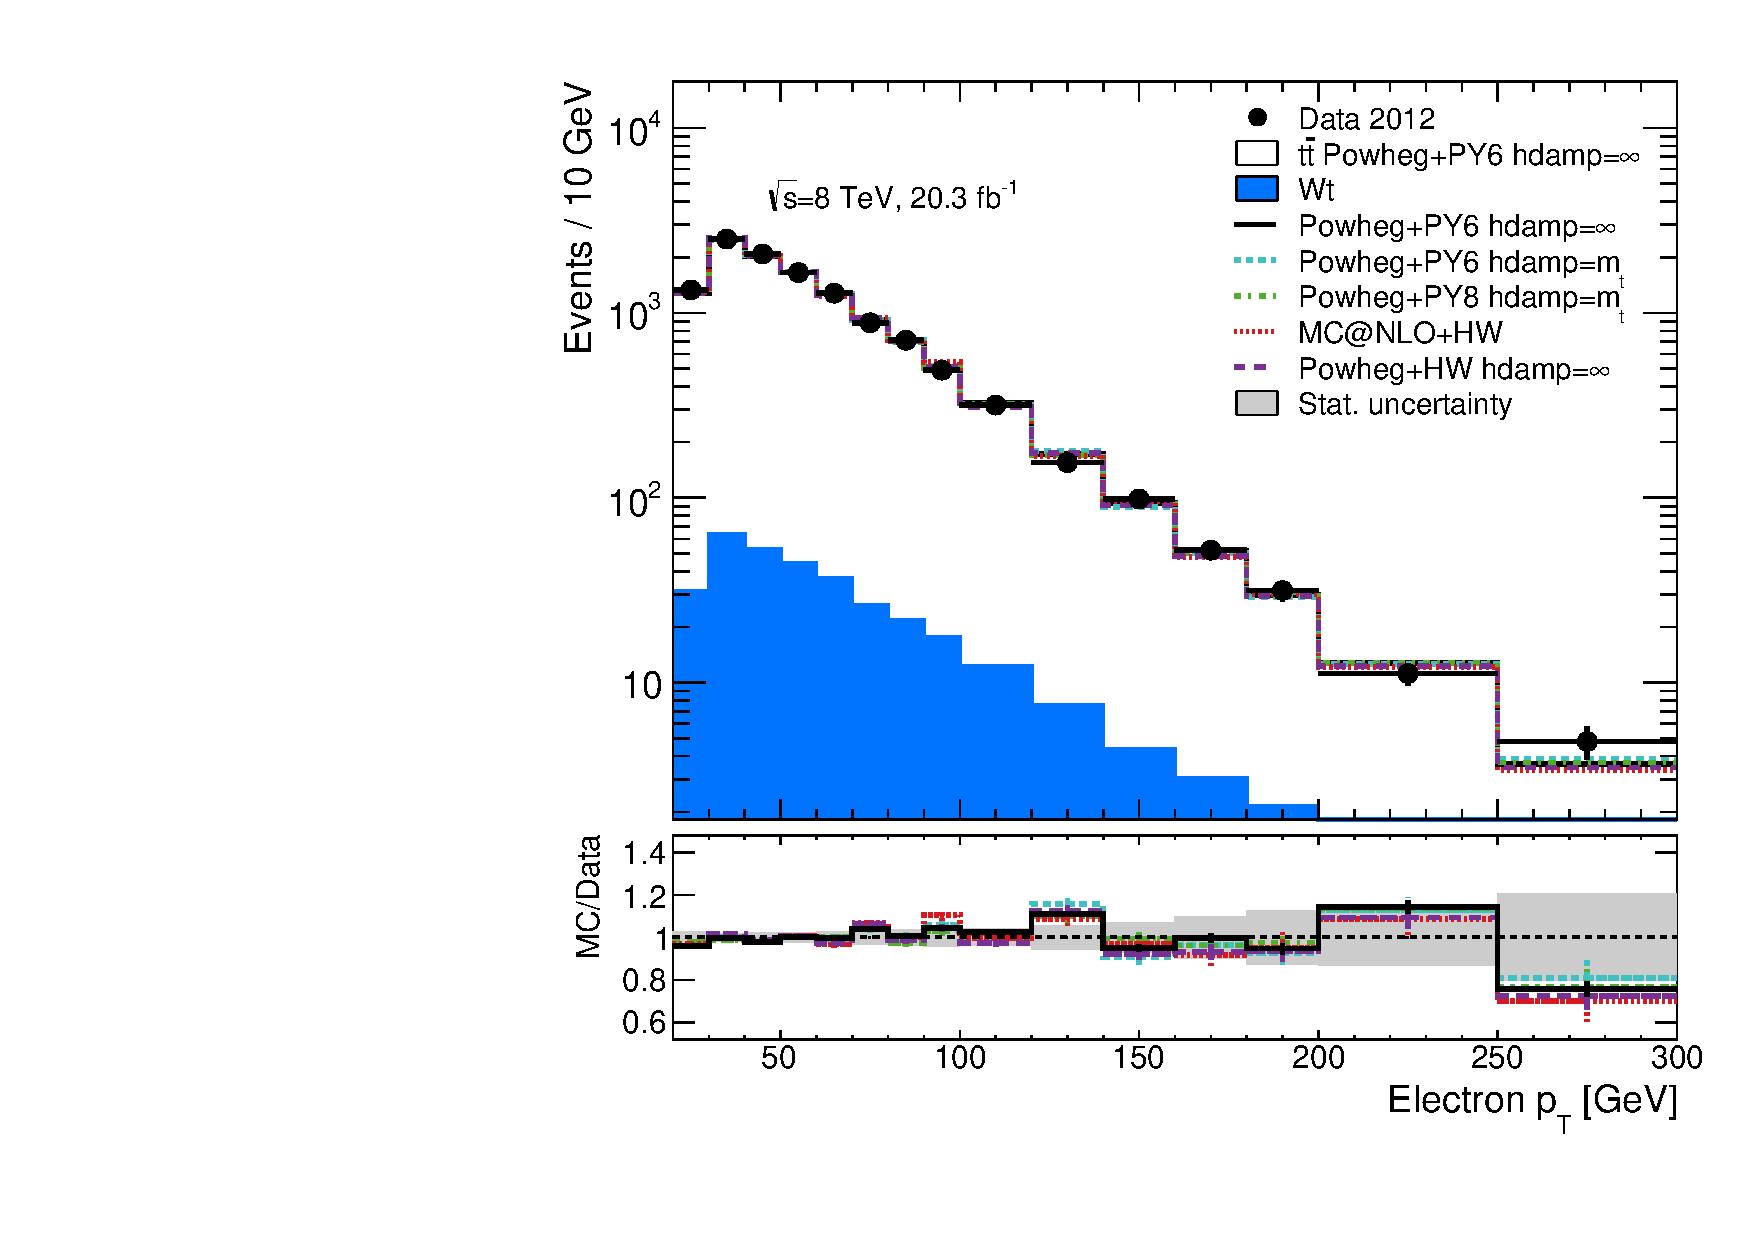
\includegraphics[width=\textwidth]{fig/MCComp/NLO/ElecPt.pdf}
\end{subfigure}
\begin{subfigure}[]{0.45\textwidth}
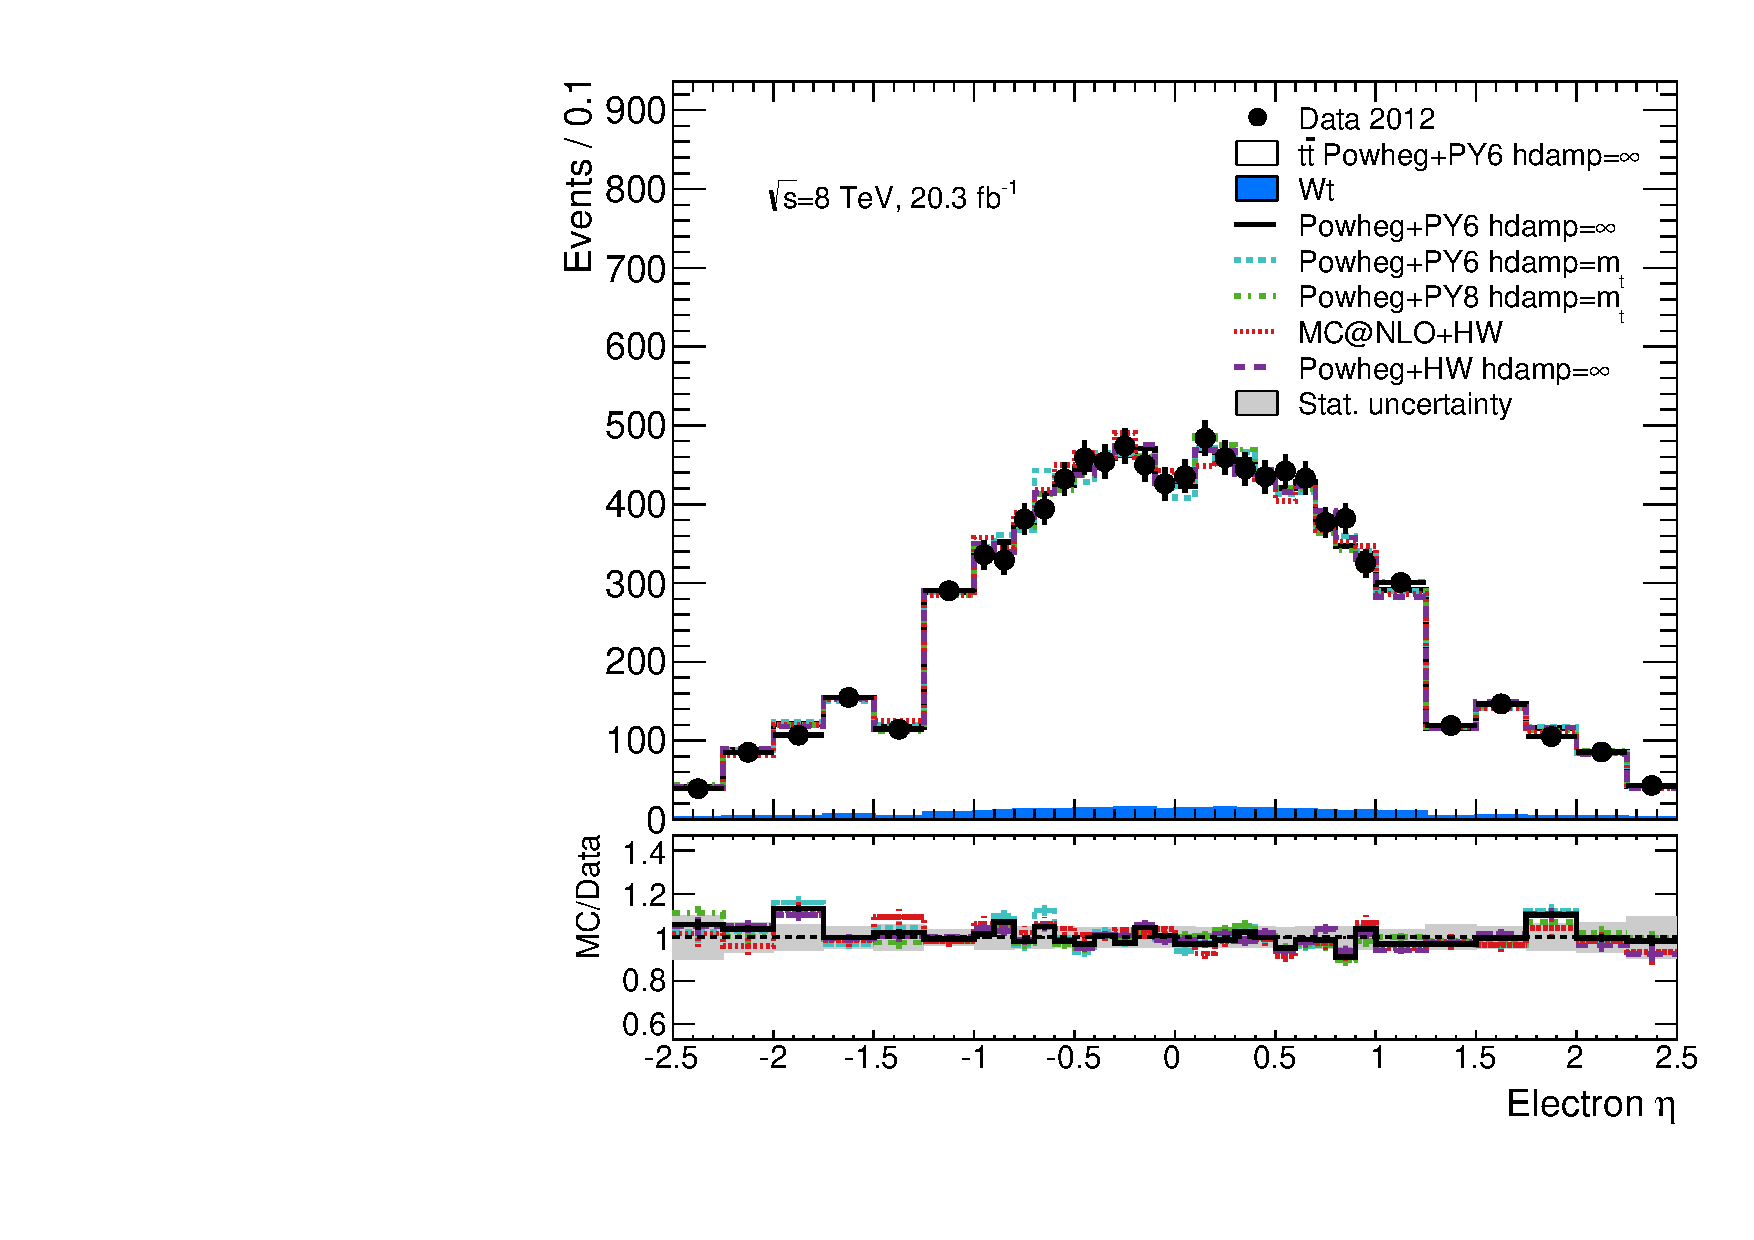
\includegraphics[width=\textwidth]{fig/MCComp/NLO/ElecEta.pdf}
\end{subfigure}
\\
\begin{subfigure}[]{0.45\textwidth}
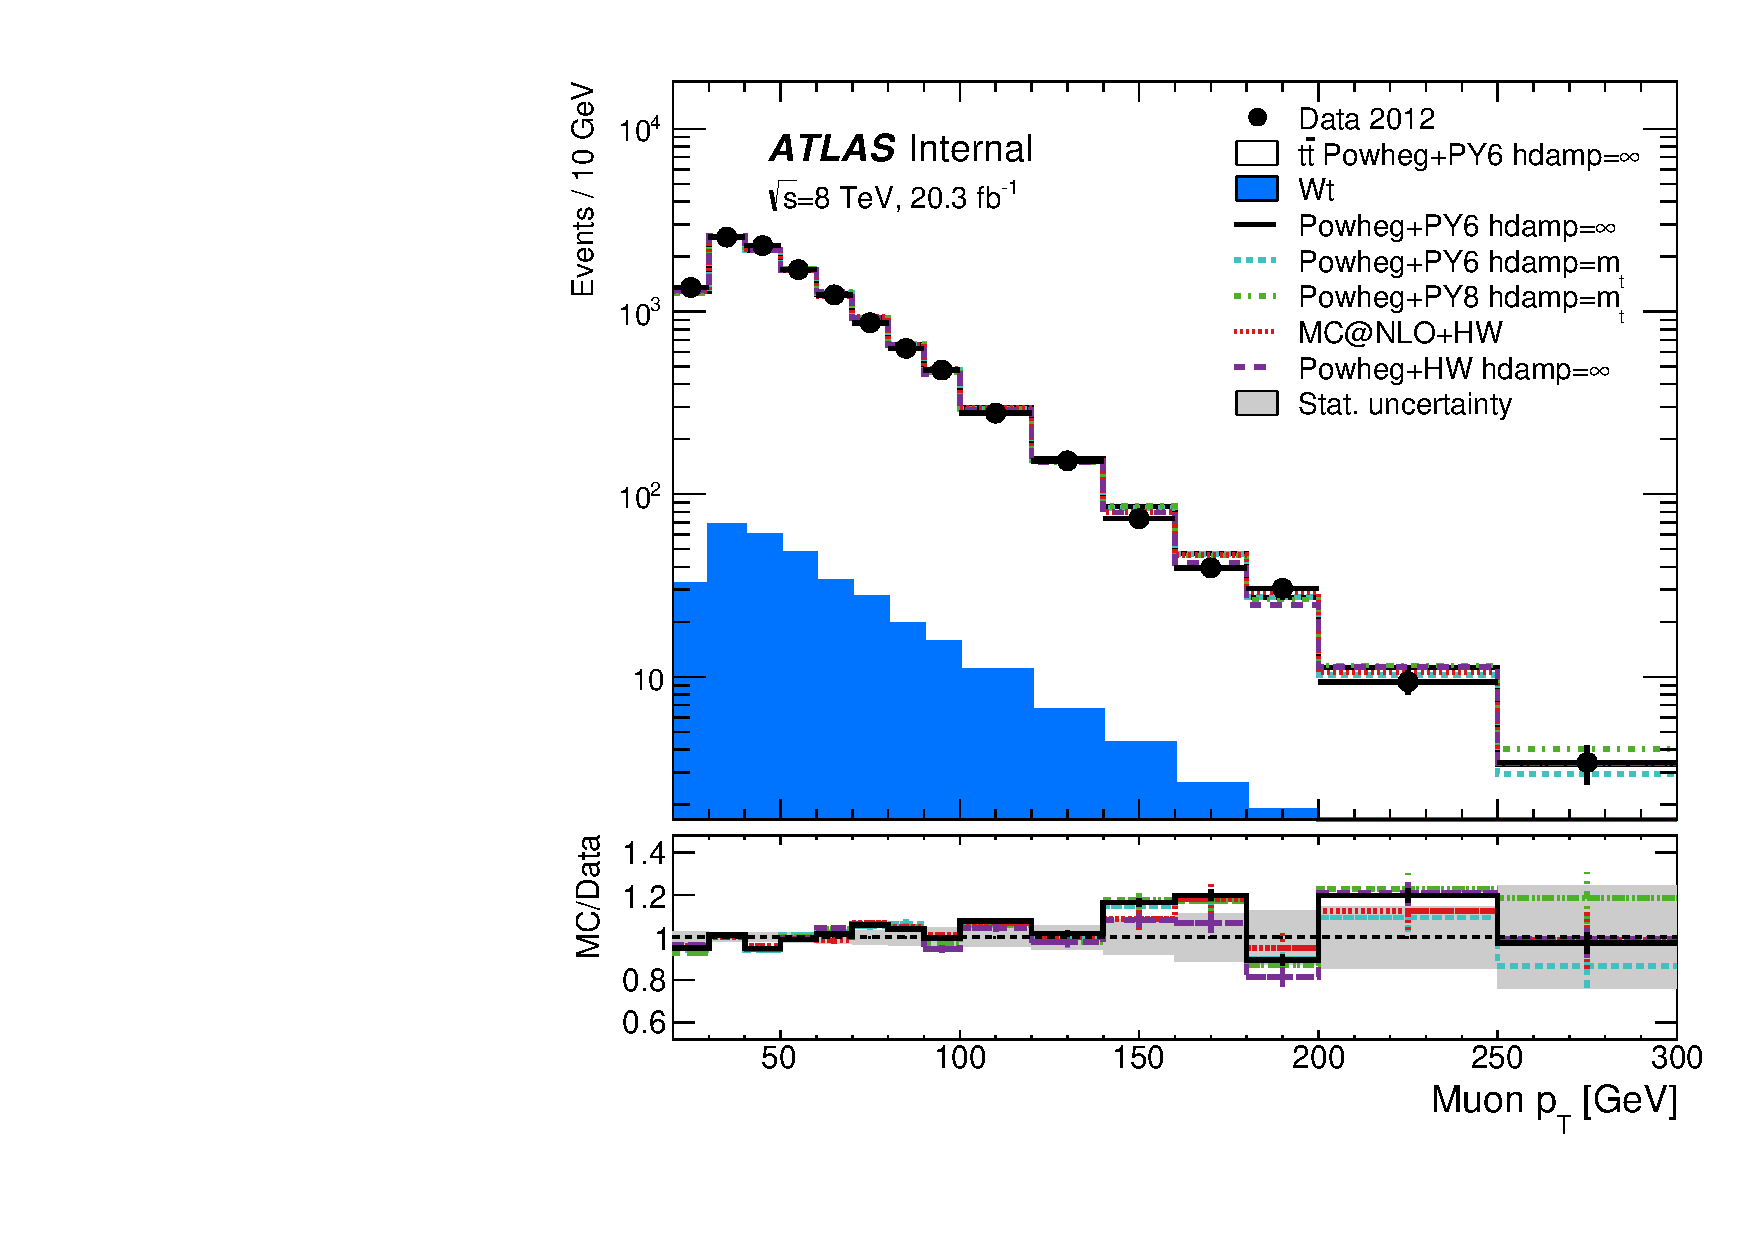
\includegraphics[width=\textwidth]{fig/MCComp/NLO/MuPt.pdf}
\end{subfigure}
\begin{subfigure}[]{0.45\textwidth}
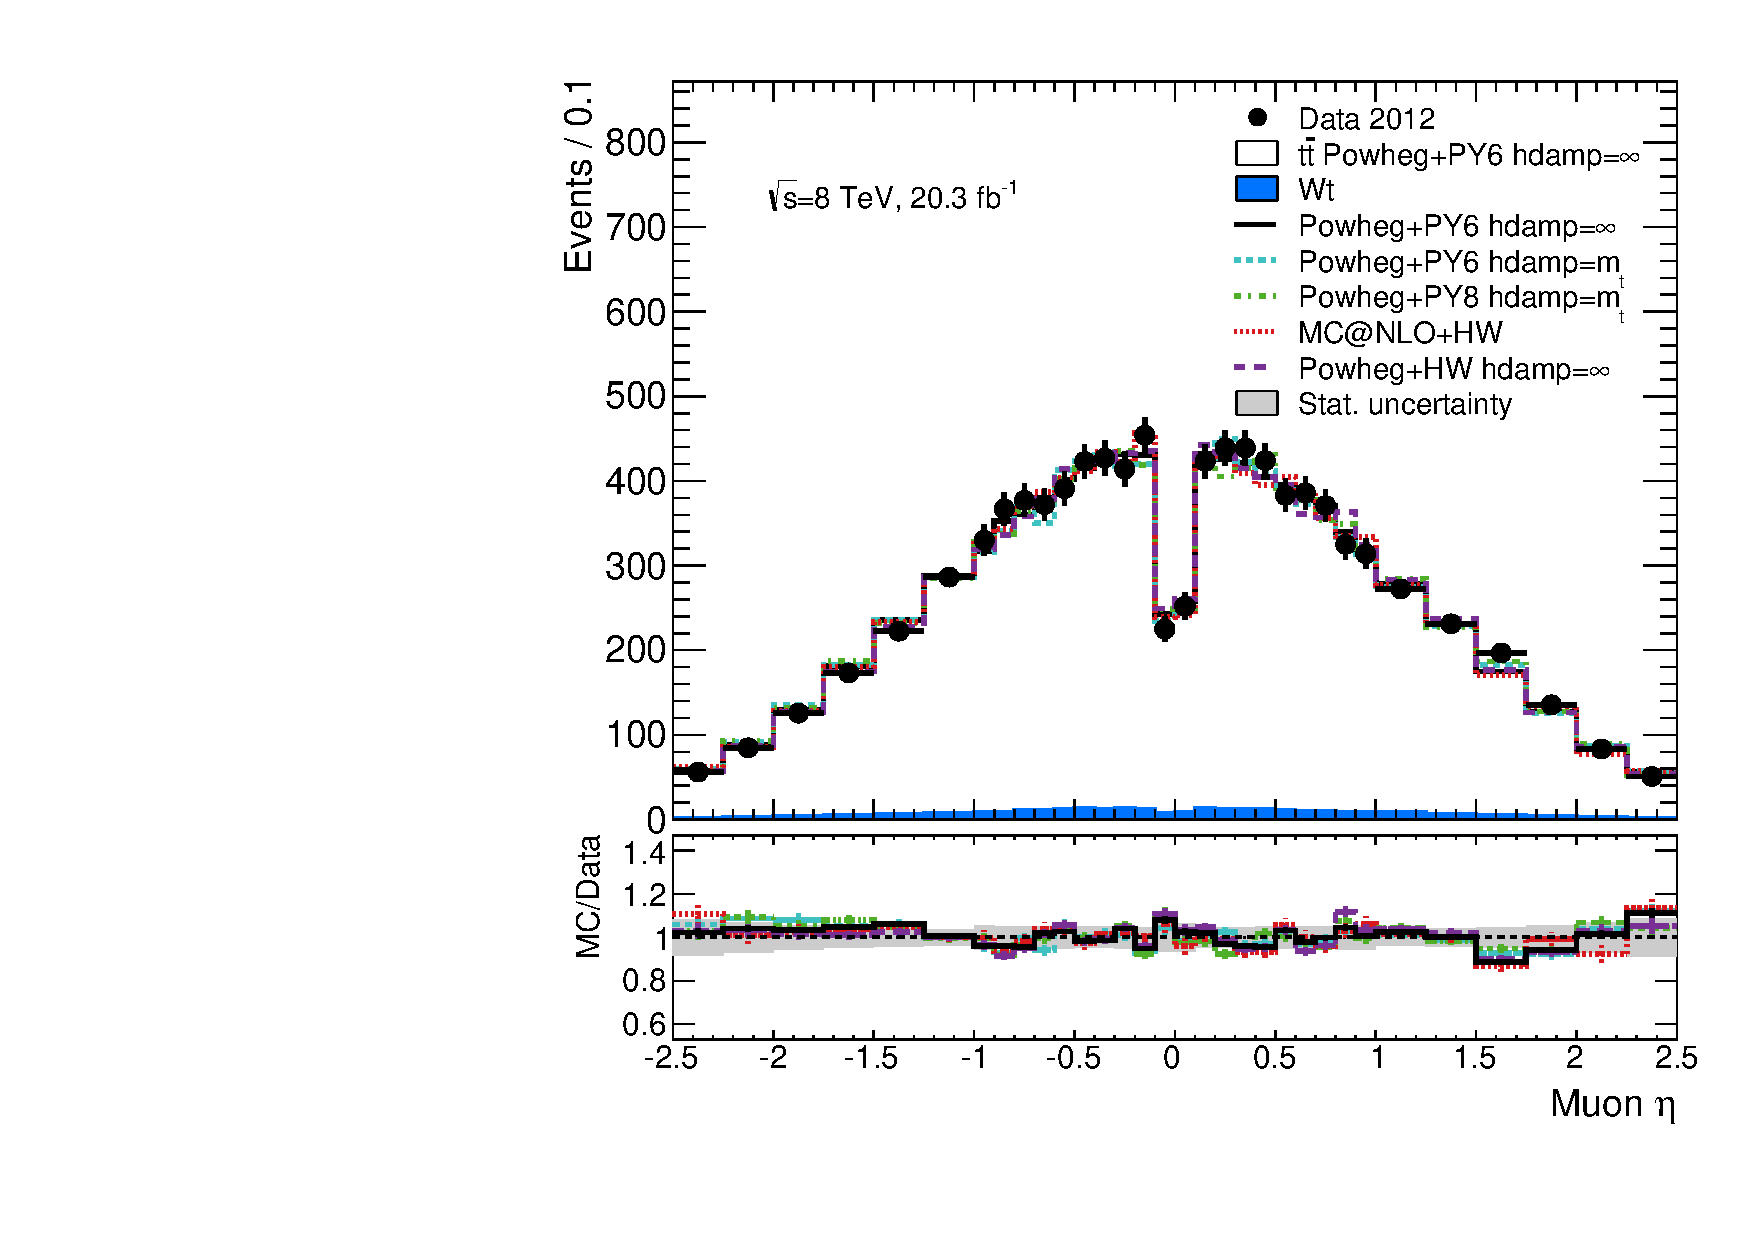
\includegraphics[width=\textwidth]{fig/MCComp/NLO/MuEta.pdf}
\end{subfigure}
\caption{Distributions of the transverse momentum and $\eta$ of the electron and muon in events with an opposite sign $e\mu$ pair and at least 2 $b$-jets in data and simulation. The distributions in data are compared to simulation normalized to data yields (see scale factors in Table~\ref{t:ttgen}). The ratio of different MC samples to data is shown with error bars corresponding to the MC statistical uncertainty and a shaded band corresponding to the data statistical uncertainty.}
\label{fig:emu}
\end{figure}

\begin{figure}
\centering
\begin{subfigure}[]{0.45\textwidth}
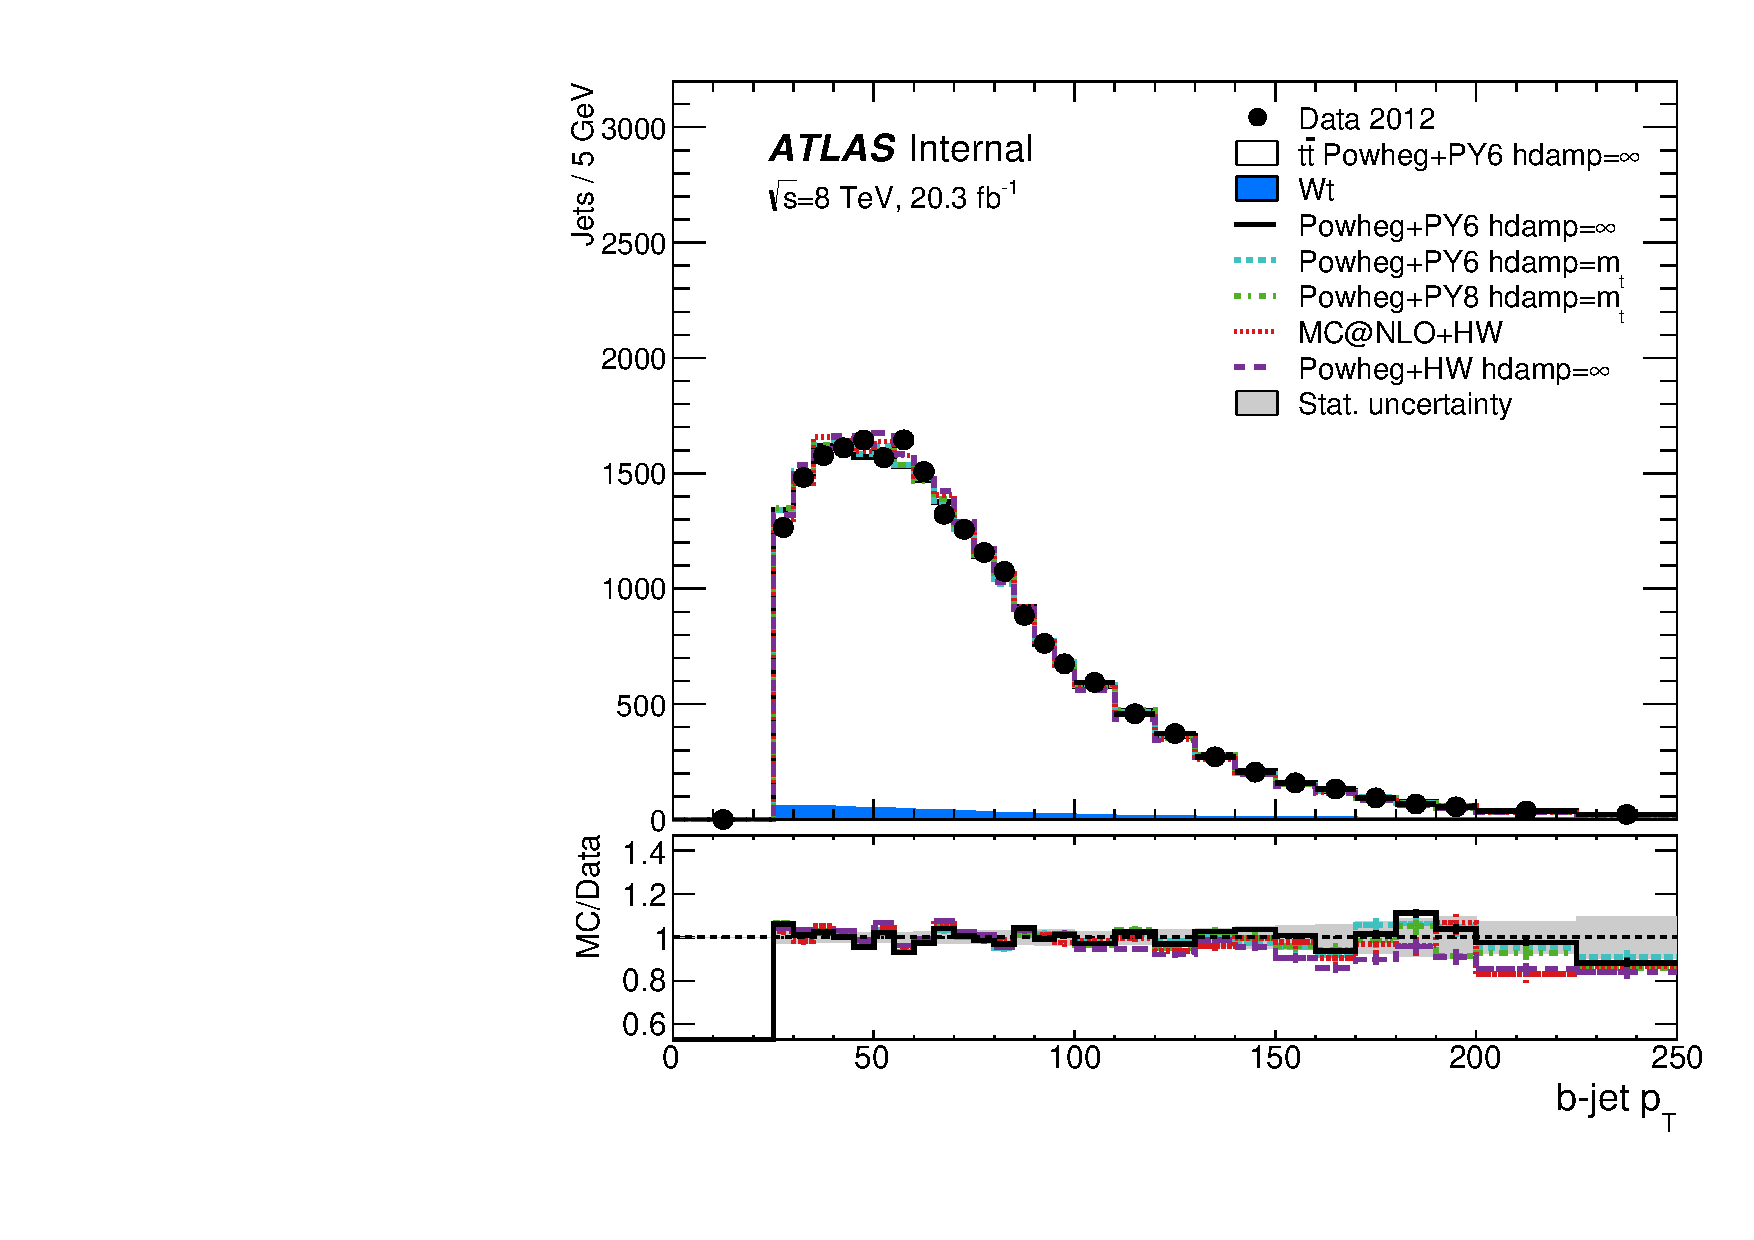
\includegraphics[width=\textwidth]{fig/MCComp/NLO/BJetPt.pdf}
\end{subfigure}
\begin{subfigure}[]{0.45\textwidth}
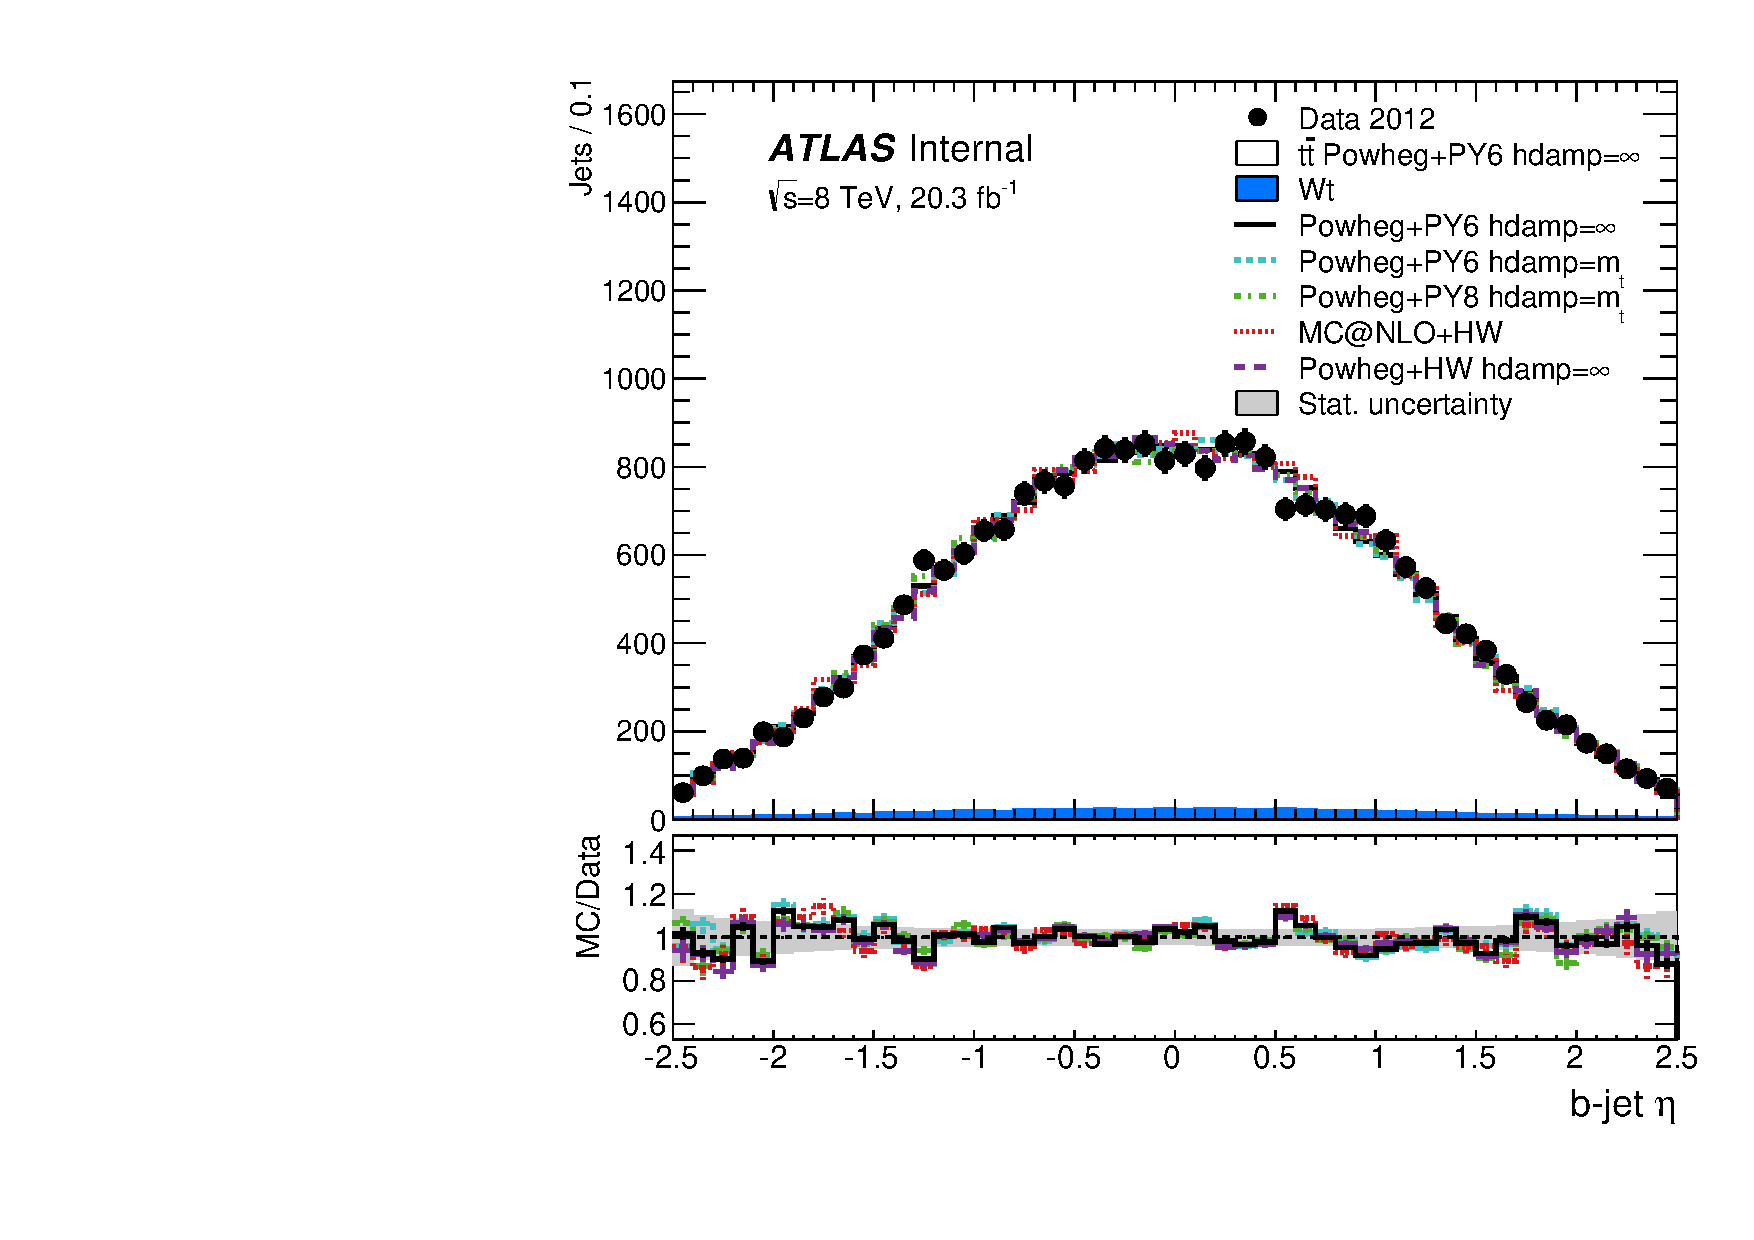
\includegraphics[width=\textwidth]{fig/MCComp/NLO/BJetEta.pdf}
\end{subfigure}

\caption{Distributions of the transverse momentum and $\eta$ of the $b$-jets in events with an opposite sign $e\mu$ pair  and at least 2 $b$-jets in the 2012 data. The distributions in data are compared to simulation, normalized to the same number of events as in the data  (see scale factors in Table~\ref{t:ttgen}).. In events where more than two $b$-jets are reconstructed, the two highest \pt $b$-jets are selected and the remaining $b$-jet is classified as an extra jet (see Chapter ~\ref{ch:extrajets}). The ratio of different MC samples to data are shown with error bars corresponding to the MC statistical uncertainty and a shaded band corresponding to the data statistical uncertainty. Systematic uncertainties are not shown.}
\label{fig:bjet}
\end{figure}


\chapter{Reconstruction of extra jets}
\label{ch:extrajets}

The goal of this analysis is to study additional jets in events that pass the selection criteria described in Chapter~\ref{ch:event}. 
Jets in selected events are divided into two categories: the two $b$-jets used for event selection and any additional `extra' jets. In simulated data, this categorization is done independently for truth jets and reconstructed jets. The $b$-jets are required to have $|\eta|$ $<$  2.5.  Extra jets are required to have  $|\eta|$ $<$  4.5. The final measurement of the extra jets will be corrected to the fiducial region $p_{T}^{jet} > 25$~\GeV.

\section{Matching criteria}
As described in Chapter~\ref{ss:tmatching}, a geometric algorithm matches reconstructed jets to truth jets. The $b$-jets are matched before the extra jets and no two reconstructed jets are allowed to match to the same truth jet. Though required to have reconstructed $\pt>25 \GeV$, reconstructed jets are matched to truth jets with $\pt>10 \GeV$. This procedure allows the unfolding to account for migration over the selection boundary.

In the $\sim 2\%$ of events with more than two reconstructed $b$-jets, the two reconstructed jets with the highest MV1 weights are classified as the selected $b$-jets and the remaining jets are treated as extra jets. In the events that contain more than two reconstructed $b$-jets, this prescription selects $b$-jets that are matched to the top decay products with 74\% accuracy. In contrast, choosing the two highest \pt $b$-jets in these same events selects $b$-jets from the top decay 68\% of the time. In simulated events with exactly 2 reconstructed $b$-jets, 96\% of selected $b$-jets descend from the top quark; the remainder are consistent with mistagged~\cite{btagmiscal} non $b$-jets. Such misclassification of $b$-jets is accounted for in the correction procedure described in Chapter~\ref{ch:unfolding}.



\section{Background contributions to extra jets}
\label{ss:pileup}
In the baseline MC sample, approximately 4\% of the events contain an \textit{unmatched} jet (see Chapter~\ref{ss:tmatching}). The RooUnfold package used to unfold the data does not properly handle \pT-dependent background subtraction. Therefore, the unfolding response matrix is constructed using only matched jets. Unmatched jets are defined to be background and are subtracted from the data before unfolding. 
Unmatched jets can result from two sources: 
\begin{description}
\item[Pileup]: Jets coming from additional proton-proton collisions within the same bunch crossing.
\item[False]: Jets observed in the reconstruction that arise from detector effects or jets resulting from reconstruction pathologies such as a when a single truth jet is split into two reconstructed jets or when the $\eta-\phi$ positions of the truth and reconstructed jets differ by more than the matching distance of 0.4.
\end{description}
 %\footnote{Because the minimum truth jet \pt\ is lowered to 10~\GeV\ during the matching procedure, cases where resolution smearing matches a reconstructed jet above the 25~\GeV\ \pt\ cut to a truth jet below it are not considered unmatched jets.} 
The  procedures used to estimate the rate of these two types of backgrounds are outlined below.

\subsection{Pileup jets}


The ATLAS simulation describes the effect of pileup on hard-scatter jets well~\cite{jetpile}. However, the multiplicity of pileup jets has not been as fully validated, especially in the region $2.4 <  |\eta| < 4.5$.  Ideally, the pileup rate could be
estimated using the ATLAS pileup overlay simulation framework.  In this framework,
zero bias events from data are combined with simulated hits for the hard scattering event
and the digitization and reconstruction are performed on the combined sample. However,
no sample with sufficiently high statistics presently exists.  

A higher statistics alternative to the overlay sample can be constructed using a hybrid technique.
This hybrid technique takes as its input files 
from the baseline simulation and from the ZeroBiasOverlay data steam~\footnote{Real data events collected with a zero-bias trigger that selects purely random events. The events from this stream can be combined or ``overlaid'' on a generated process to simulate pileup. See Ref.~\cite{minbias} for more information.}.  
Unmatched jets are removed from the baseline simulation
and the matched jets are combined with reconstructed jets from the zero bias data.  

To properly estimate the pileup rate, the input ZeroBiasOverlay data must be luminosity-weighted
to match the data.  This weighting is done as follows.  First, the run number and luminosity block number 
for all events passing the \emubb\ data event selection is tabulated.  Second, data from the ZeroBiasOverlay
stream is skimmed to keep only those run and luminosity block pairs present in the selected data.
Third, \ttbar\ MC events are analysed.
The $e$,$\mu$, \bjet s, and truth-matched additional jets are kept and the unmatched
additional jets are deleted.  For each MC event, a ZeroBiasOverlay data event is 
randomly selected from the skimmed data.
The distribution of these ZeroBias events is forced to sample the list of run and luminosity block numbers
to match the distribution for the \emubb\ data.  The reconstructed jets in the selected ZeroBiasOverlay
event are added to the \ttbar\ MC event record.  An overlap 
removal procedure removes zero bias jets that overlap hard scatter jets.
If a zero bias jet overlaps a lepton, then the event is removed from the sample. 
This hybrid sample provides the baseline estimate of the pileup contribution to the 
extra jet distributions. 

The dependence of the extra jet rate on the average number of interactions per bunch crossing ($\mu$) in the signal sample is used to validate this estimate. %Details of this validation are provided in Appendix~\ref{app:pileup}.
 Figure~\ref{fig:pileupjets} shows an example of this procedure for (a) central and (b) forward jets for the lowest jet \pt\ bin used in this analysis. The figure shows the mean number of jets in events passing the baseline selection as a function of $\mu$ and the pileup contribution estimated from the ZeroBiasOverlay stream. Before pileup subtraction, the number of jets depends on $\mu$, with a larger dependence observed in the forward $\eta$ region where the JVF cut can not be used. After subtraction of the pileup using the estimate from the ZeroBiasOveray stream, this $\mu$ dependence is eliminated. For this \pt\ bin, the estimated number of pileup extra jets per
event is 0.005 (0.016) in the central(forward) region. 
%Integrated over all \pt and $\eta$, the pileup fraction is ZZ. 
The pileup rate decreases with jet \pT\ and is estimated to be below 0.002 for jets with $\pt>50$~\GeV.
Systematic uncertainties on this pileup estimate are discussed in Chapter~\ref{ss:sysbkg}.
 
 \subsection{False jets}
Reconstruction pathologies are studied using simulated data. Because the simulation event record does not contain truth information for pileup, it is not straightforward to determine what fraction of the unmatched jets derive from pileup and what fraction are the result of other detector effects. The simplest way to study the rate of false jets would be to study them in a sample simulated without pileup, but no such \ttbar\ sample exists. 

The rate of false jets is estimated by studying the $\Delta {R}$ between extra jets. While the $\eta-\phi$ position of pileup jets is uncorrelated with the position of truth jets, false jets from reconstruction pathologies should be preferentially close to truth jets (since they are derived from particles in these truth jets).  
Figure~\ref{fig:recodr} shows the distance between each reconstructed jet and the nearest additional reconstructed jet in the event ($\Delta {R}_{\text{reco jet, reco jet}}$) in simulation and in data for jets of rank=1-4. The data is in good agreement with the simulation. 
The contribution of unmatched jets at low $\Delta {R}_{\text{reco jet, reco jet}}$ is evident in the figure;
%The simulation has an excess of unmatched jets at low $\Delta {R}_{\text{reco jet, reco jet}}$ and this component 
this false jet component is needed in order to reproduce the shape observed in the data.
%, showing that the simulation properly models this background.

%While Figure~\ref{fig:recodr} validates the modeling of the separation of the extra jets, additional information is needed to estimate of the false jet rate (not from pileup).

Figure~\ref{fig:truthdr} shows the distance between each reconstructed jet and the nearest truth jet ($\Delta {R}_{\text{reco jet, truth jet}}$) for jets of rank=1-4. The presence of unmatched jets with $\Delta {R}_{\text{reco jet, truth jet}} < 0.4$ results from the requirement that each truth jet can only be matched to a single reconstructed jet, as described in Chapter~\ref{ss:tmatching}. Because the matching requires $\Delta {R}_{\text{reco jet, truth jet}} < 0.4$, all jets above this threshold are unmatched. The probability that a second (and hence, unmatched) jet is reconstructed with $\Delta {R}_{\text{reco jet, truth jet}} < 0.4$ is $\sim 0.0068$.  This number represents a lower bound on the false jet rate.

The false jet rate can be estimated in another way. Figure~\ref{fig:falsecomp} shows the number of unmatched jets per event in the baseline simulation as a function of $\mu$. These unmatched jets include both the pileup and false jet contributions, with pileup dominating at high $\mu$ and false jets at low $\mu$. The rate of false jets can be determined by fitting this distribution to a first order polynomial. The intercept of this fit predicts the false jet rate, while the slope provides the pileup rate in the simulation. The fitted intercept is $0.0075 \pm   0.0014$, which is slightly higher than the estimate obtained from $\Delta {R}_{\text{reco jet, truth jet}}$ above, but is consistent
within the statisical uncertainty on the fit.   This second technique is used to obtain the baseline false jet estimate and its uncertainty.

The false jets comprise $\sim 20\%$ of the total unmatched jets and have a \pt\ and rank dependence similar to pileup jets. These two contributions are combined and treated as a single background in the subtraction procedure.
\begin{figure}
\centering
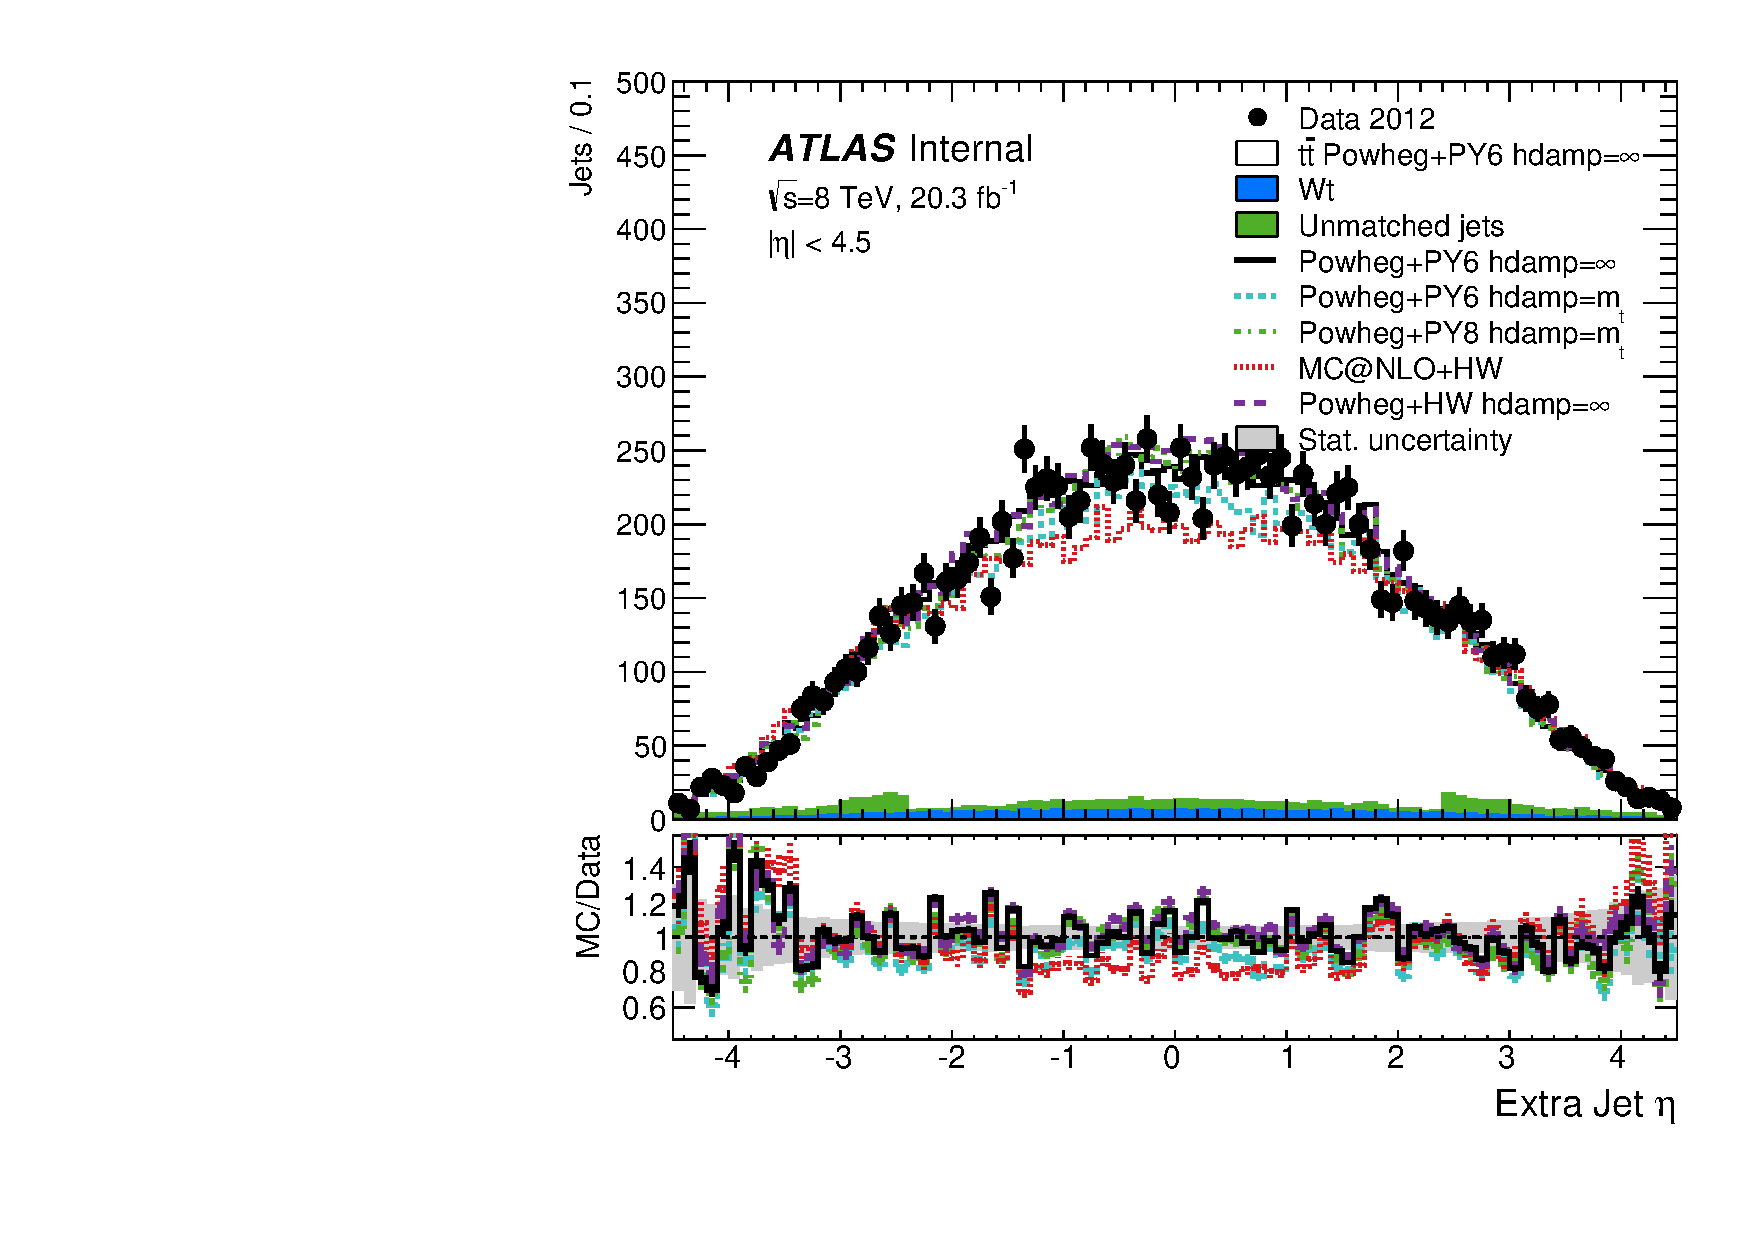
\includegraphics[width=0.9\textwidth]{fig/MCComp/NLO/ExtraJetEta.pdf}
\caption{The $\eta$ distribution of extra jets in simulation and data.}
\label{fig:jeteta}
\end{figure}

\begin{figure}
\begin{subfigure}[]{0.45\textwidth}
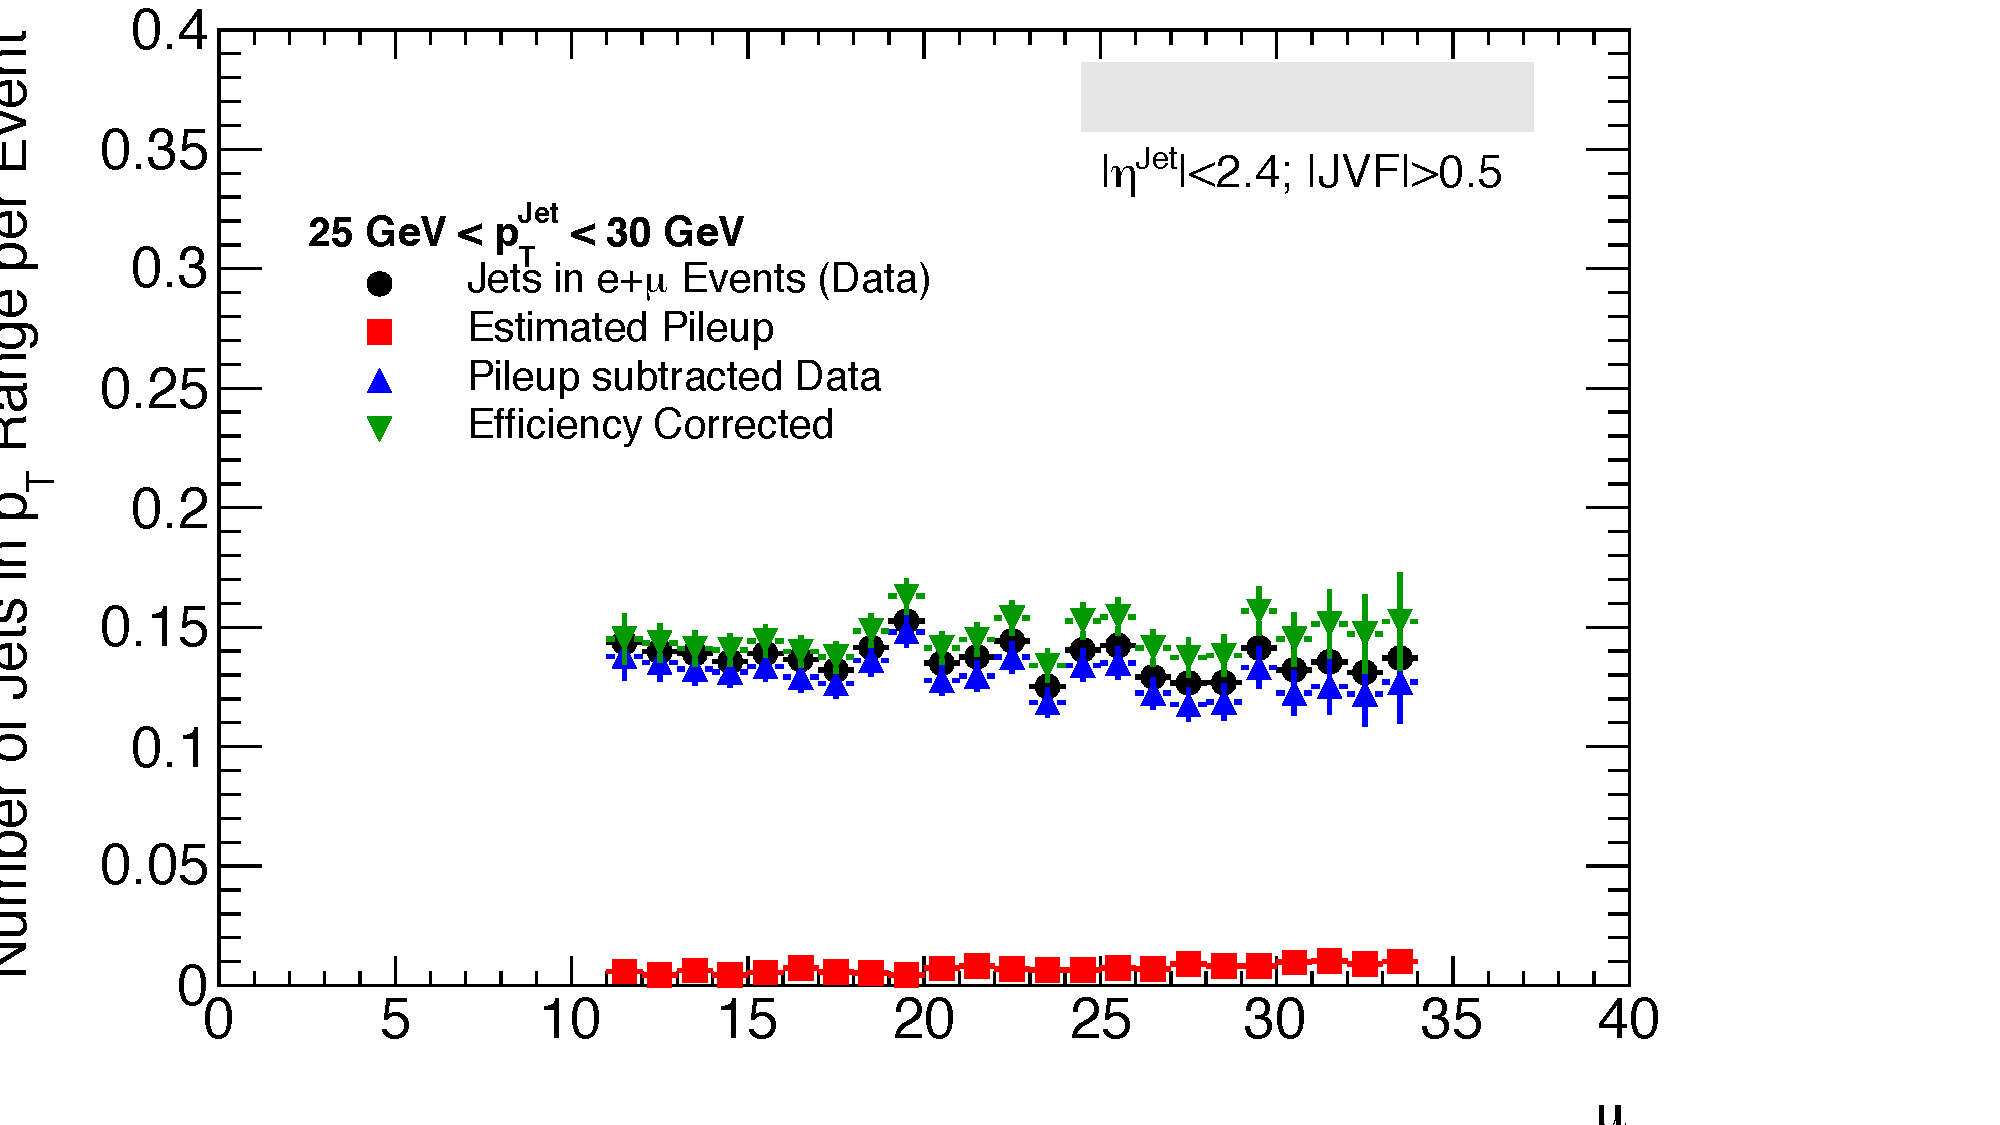
\includegraphics[width=\textwidth]{fig/Pileup/Pileup2530.pdf}
\end{subfigure}
\begin{subfigure}[]{0.45\textwidth}
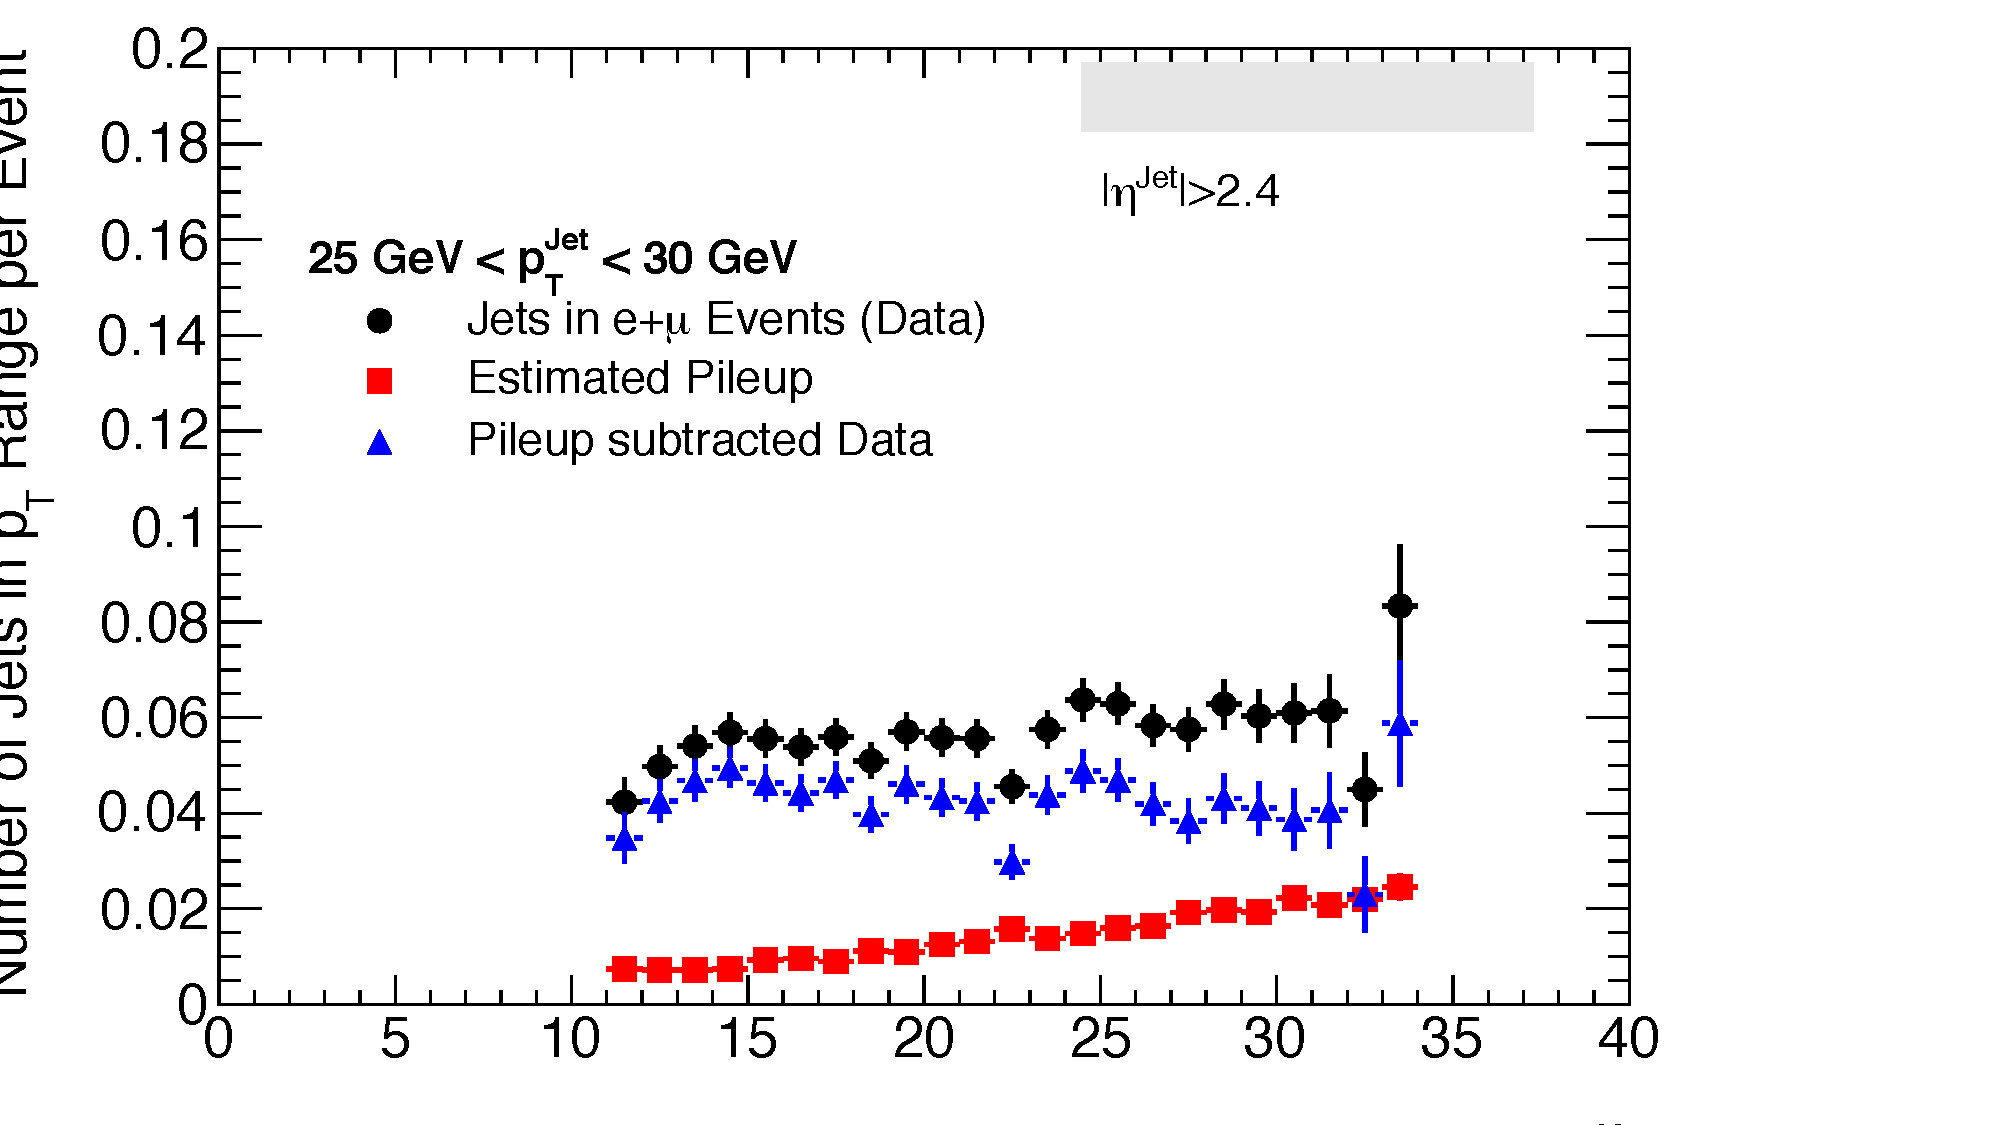
\includegraphics[width=\textwidth]{fig/Pileup/FwdPileup.pdf}
\end{subfigure}

\caption{Mean number of reconstructed jets as a function of $<\mu>$ 
for jets in the $p_T$~range $25<p_T<30$~GeV for (a) central and (b) forward jets
in data events passing the $e$-$\mu$ selection before and after correction for pileup.
Jets passing the 70\%\  MV1 b-tagging selection are removed.
The pileup rate is estimated using the ZeroBiasOverlay data stream.
The blue markers show the pileup subtracted rate before correcting
for the $<\mu>$-dependent efficiency of the JVF cut.  The green
points show the results after correction.}
\label{fig:pileupjets}
\end{figure}

\begin{figure}
\centering
\begin{subfigure}[]{0.45\textwidth}
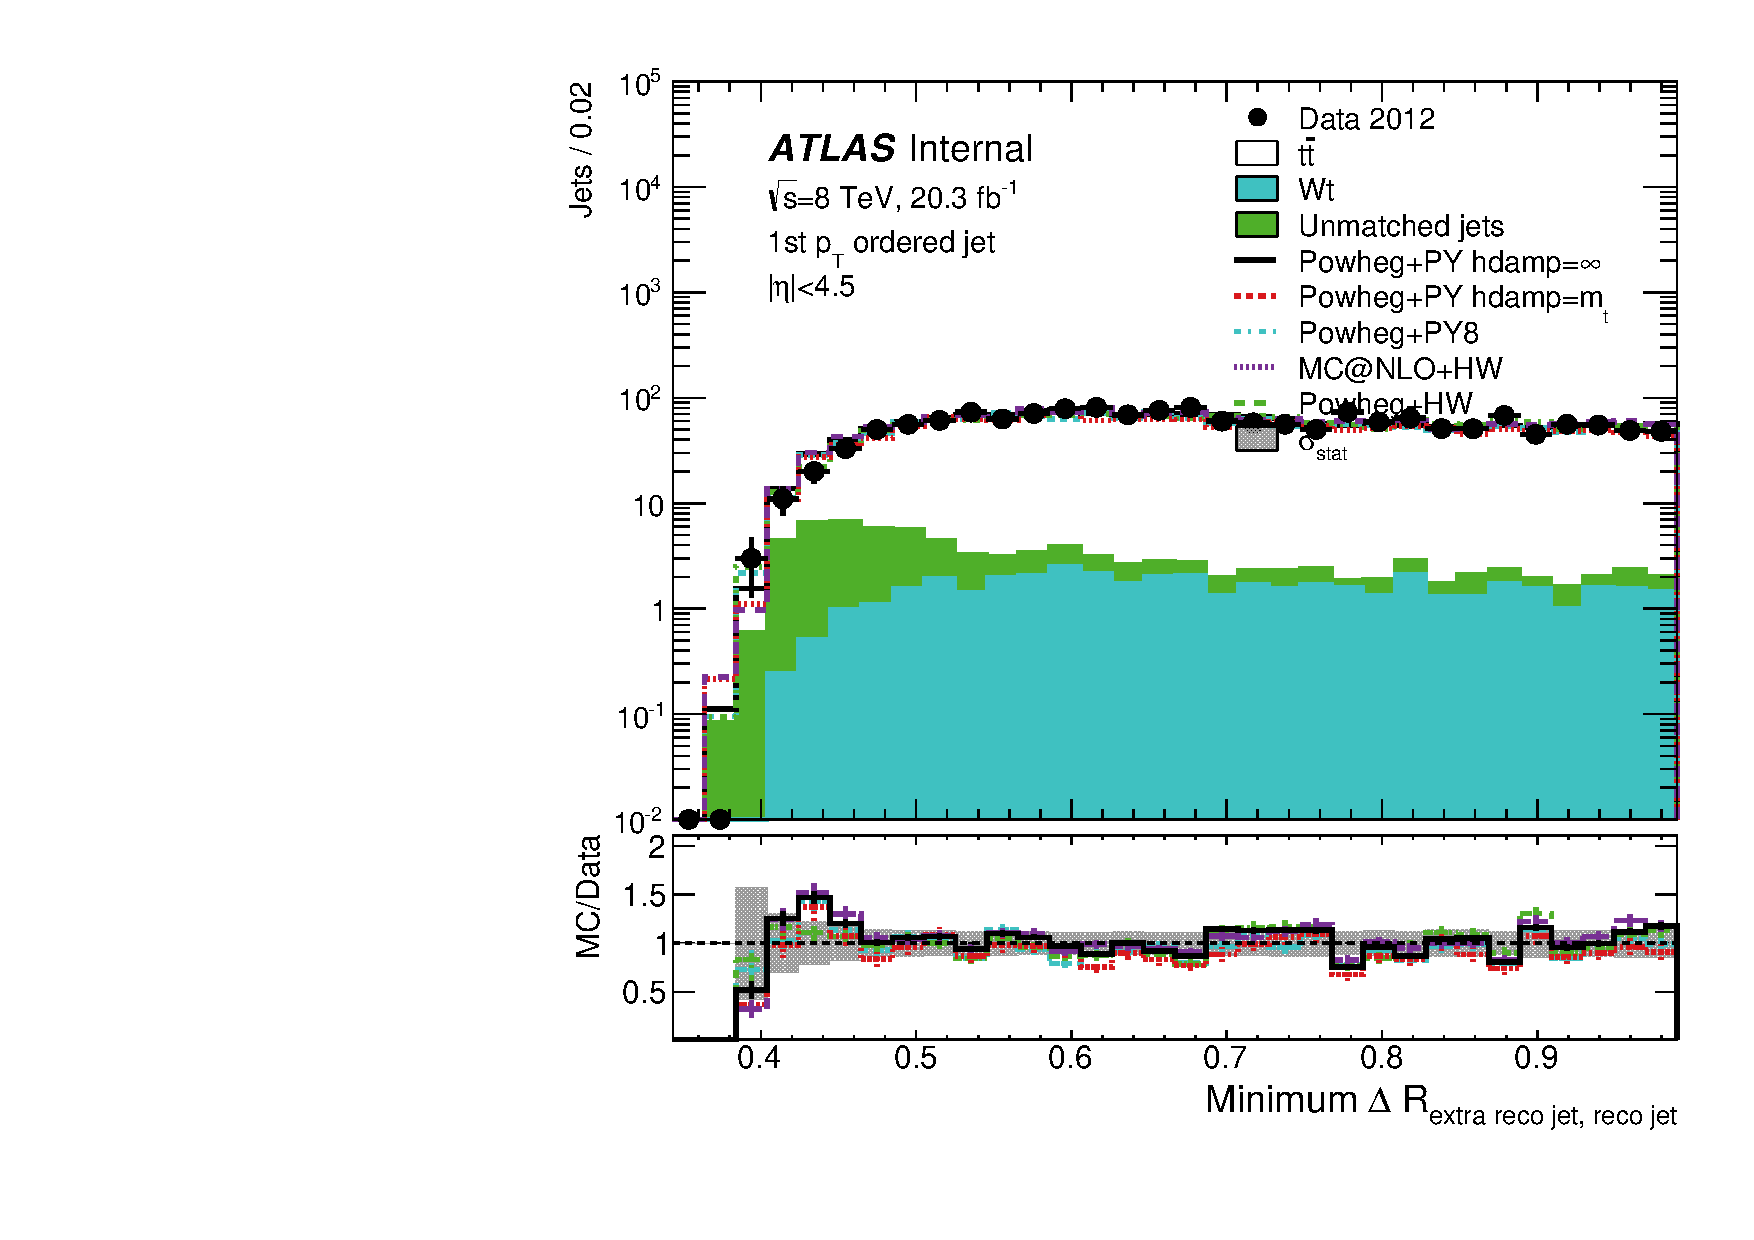
\includegraphics[width=\textwidth]{fig/MCComp/NLO/GrandPtVsRecoDRJet0.pdf}
\end{subfigure}
\begin{subfigure}[]{0.45\textwidth}
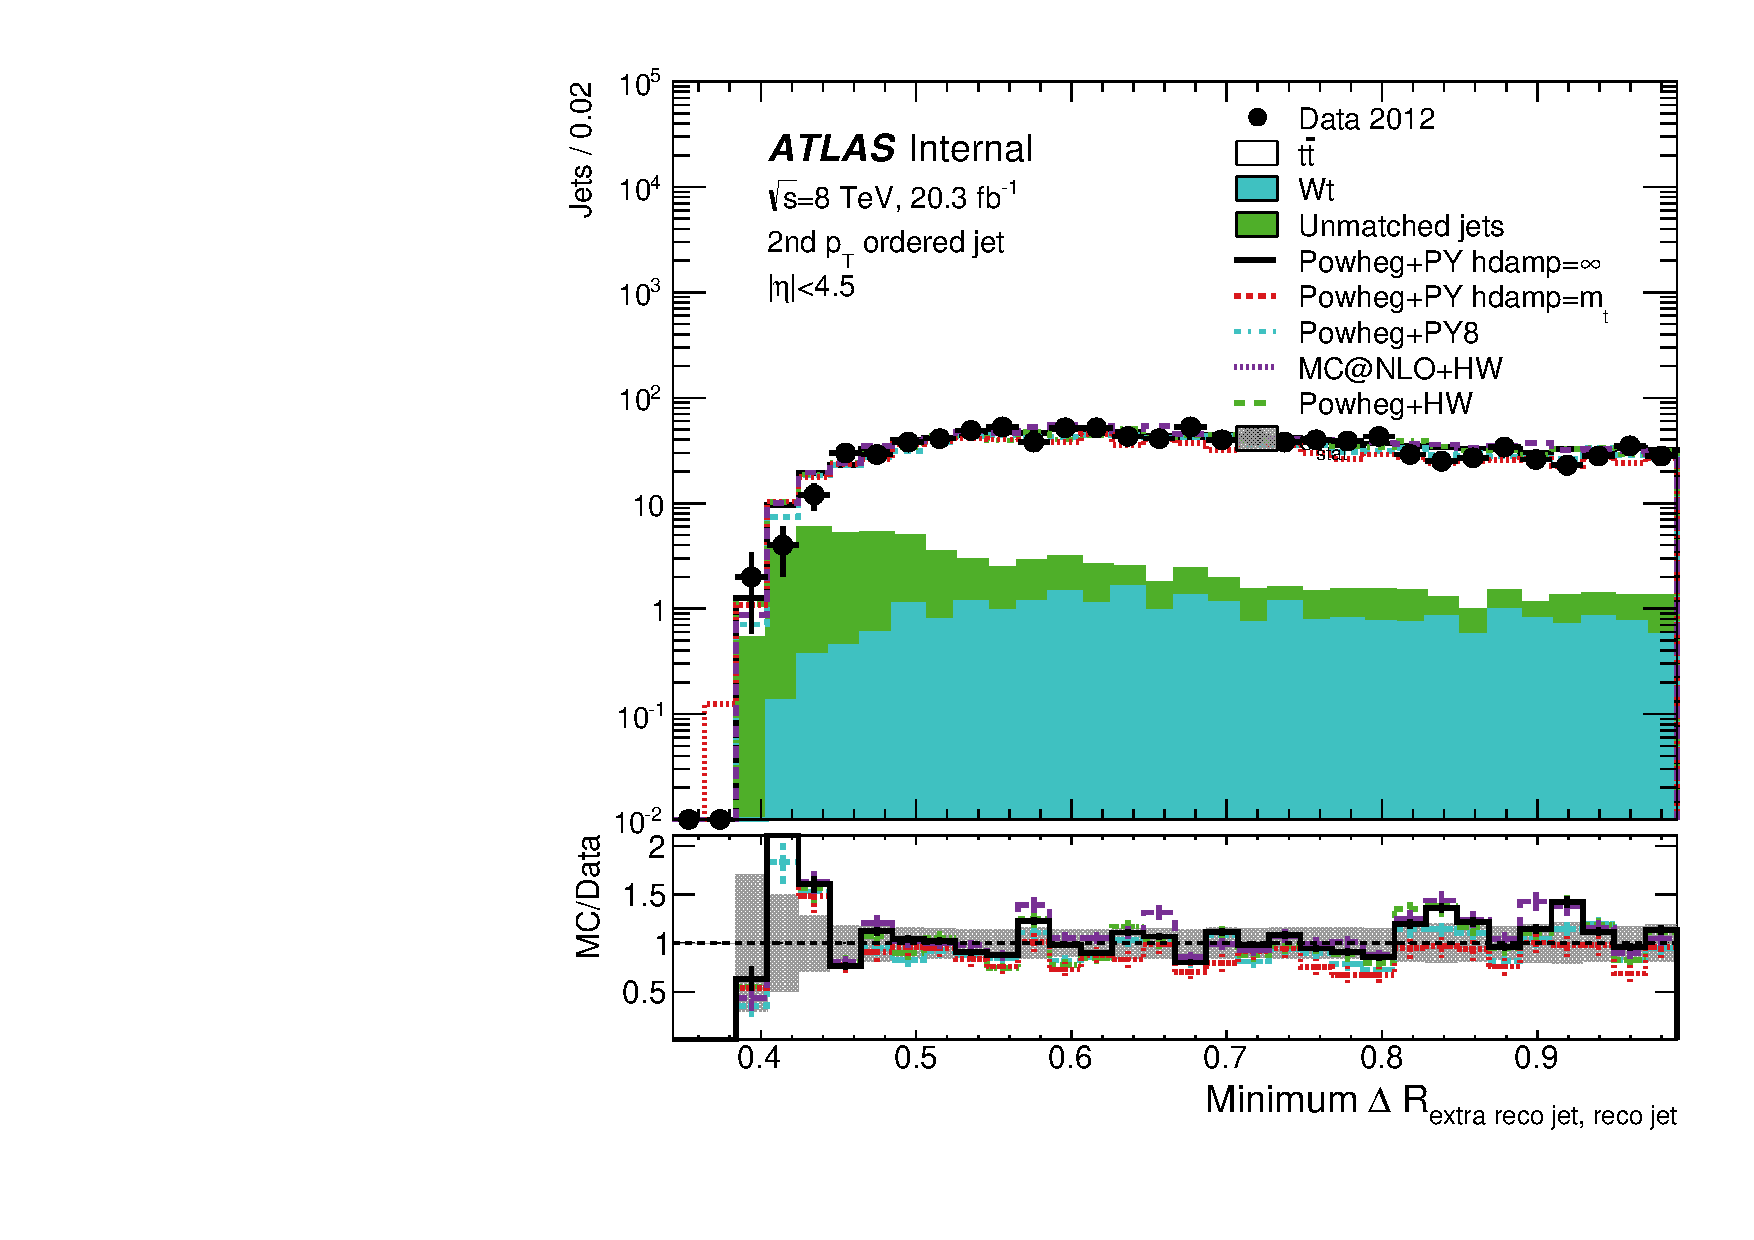
\includegraphics[width=\textwidth]{fig/MCComp/NLO/GrandPtVsRecoDRJet1.pdf}
\end{subfigure}
\\
\begin{subfigure}[]{0.45\textwidth}
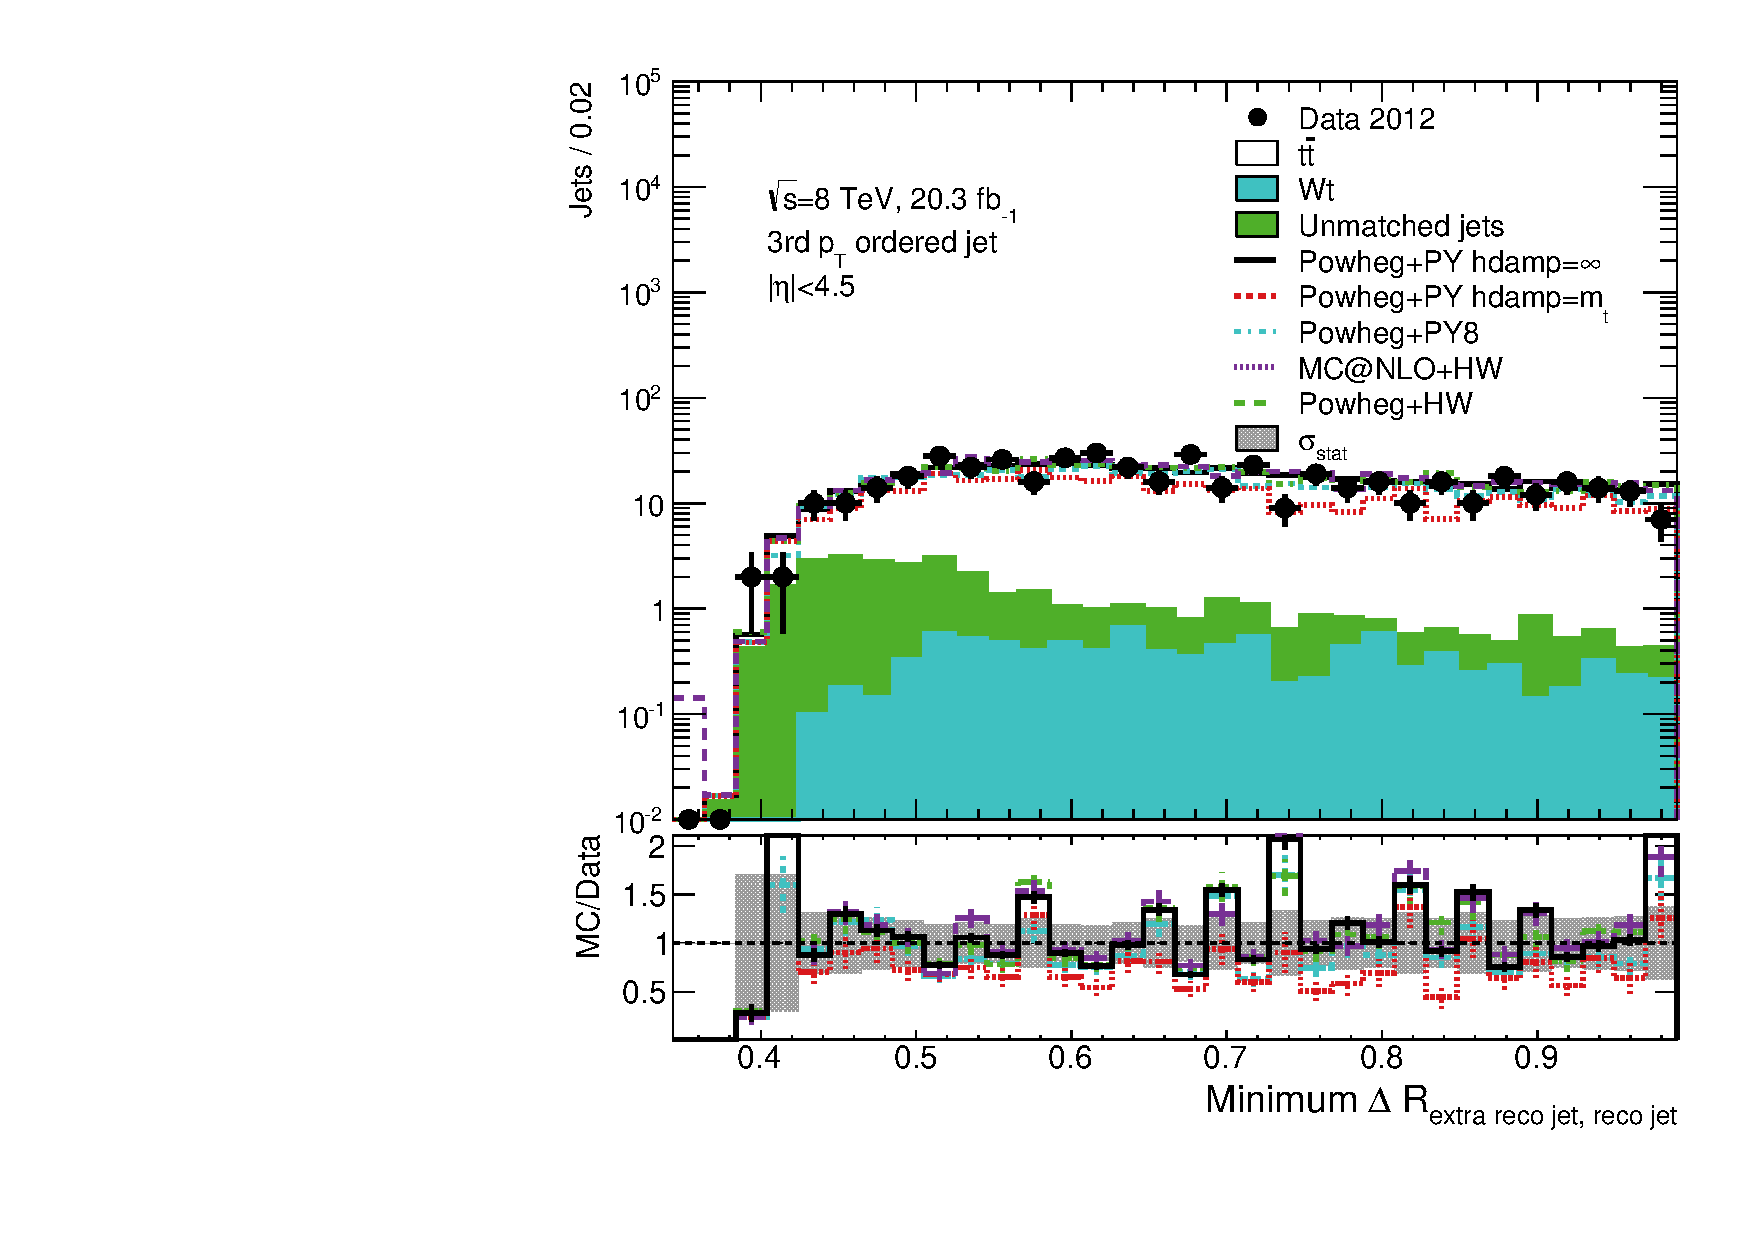
\includegraphics[width=\textwidth]{fig/MCComp/NLO/GrandPtVsRecoDRJet2.pdf}
\end{subfigure}
\begin{subfigure}[]{0.45\textwidth}
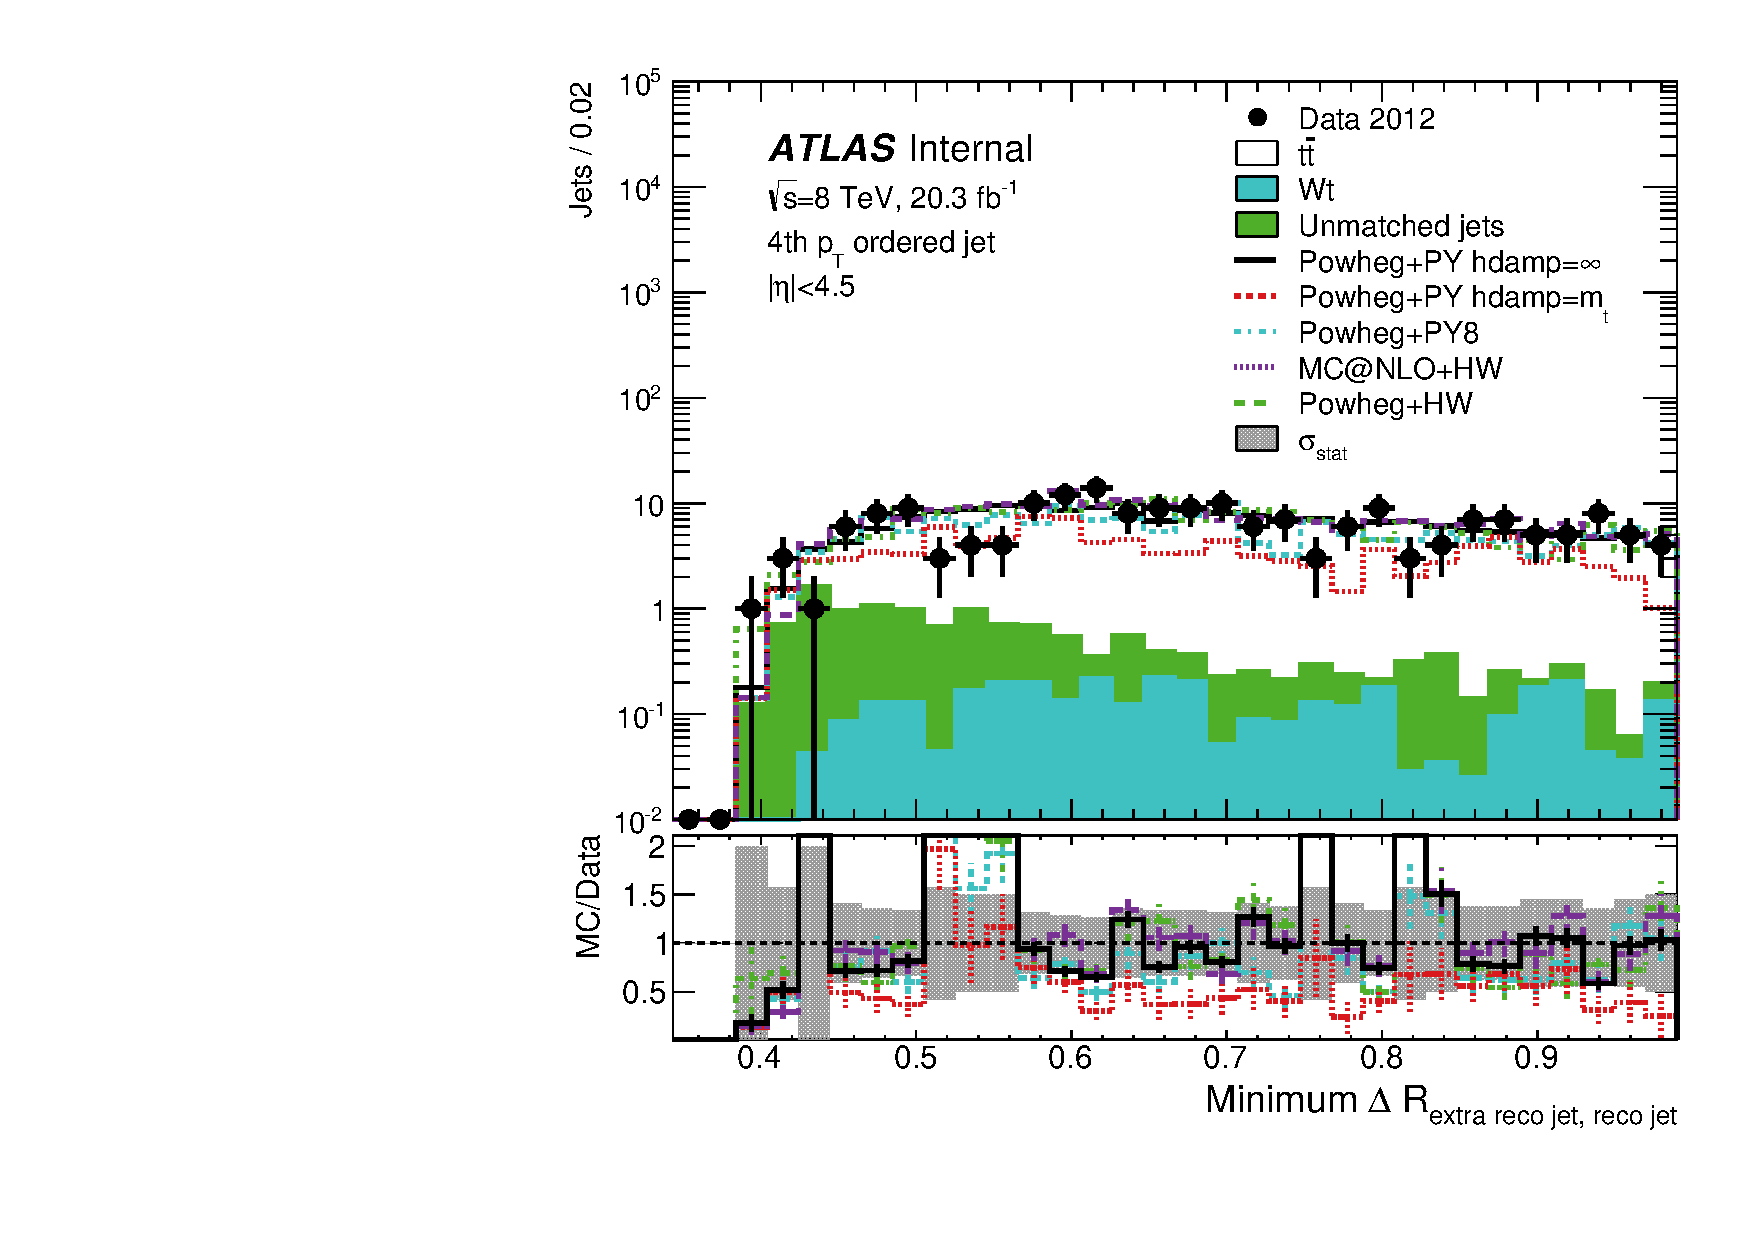
\includegraphics[width=\textwidth]{fig/MCComp/NLO/GrandPtVsRecoDRJet3.pdf}
\end{subfigure}
\caption{Distributions of minimum reconstructed $\Delta R$ betweeen extra jets in simulation and data for the the first, second, third and fourth extra jet. }
\label{fig:recodr}
\end{figure}
\begin{figure}
\centering
\begin{subfigure}[]{0.45\textwidth}
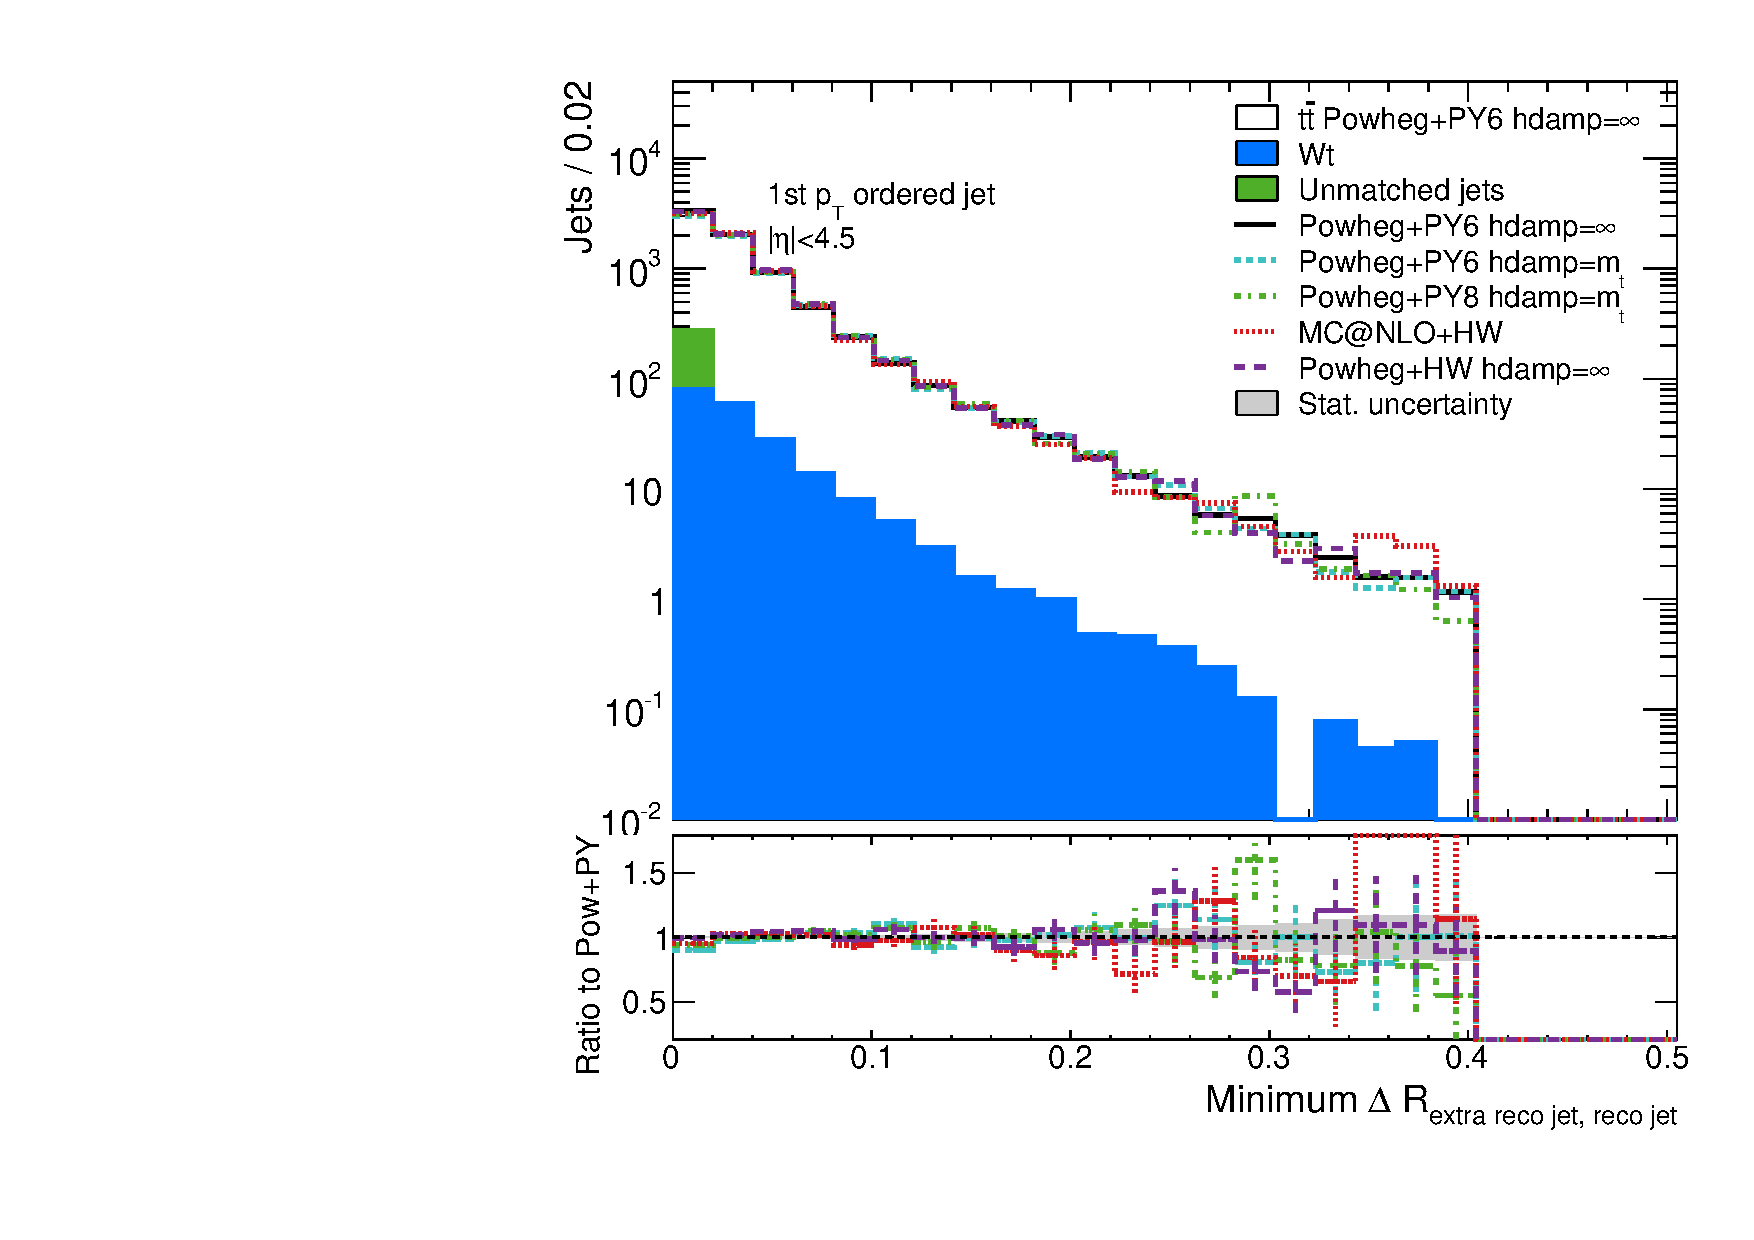
\includegraphics[width=\textwidth]{fig/MCComp/NLO/GrandPtVsTruthDRJet0.pdf}
\end{subfigure}
\begin{subfigure}[]{0.45\textwidth}
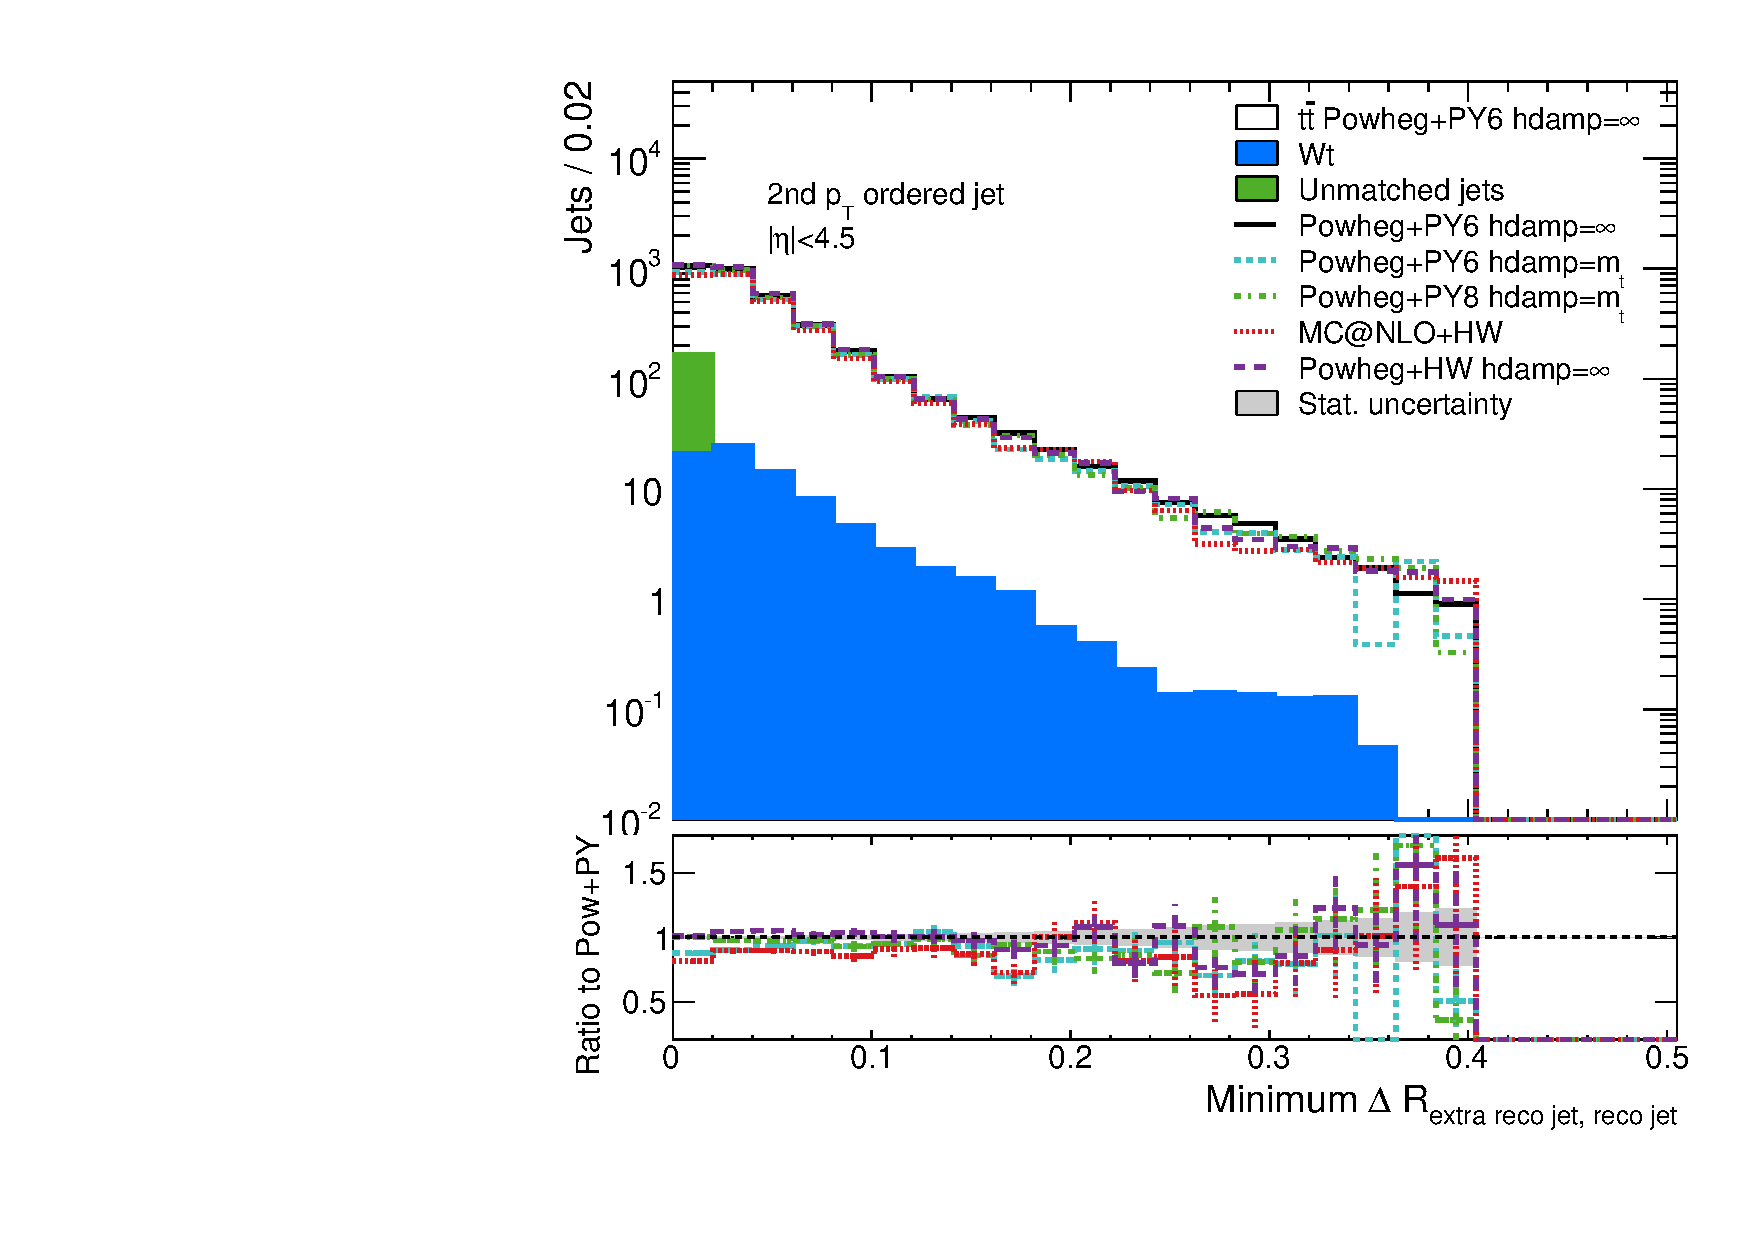
\includegraphics[width=\textwidth]{fig/MCComp/NLO/GrandPtVsTruthDRJet1.pdf}
\end{subfigure}
\\
\begin{subfigure}[]{0.45\textwidth}
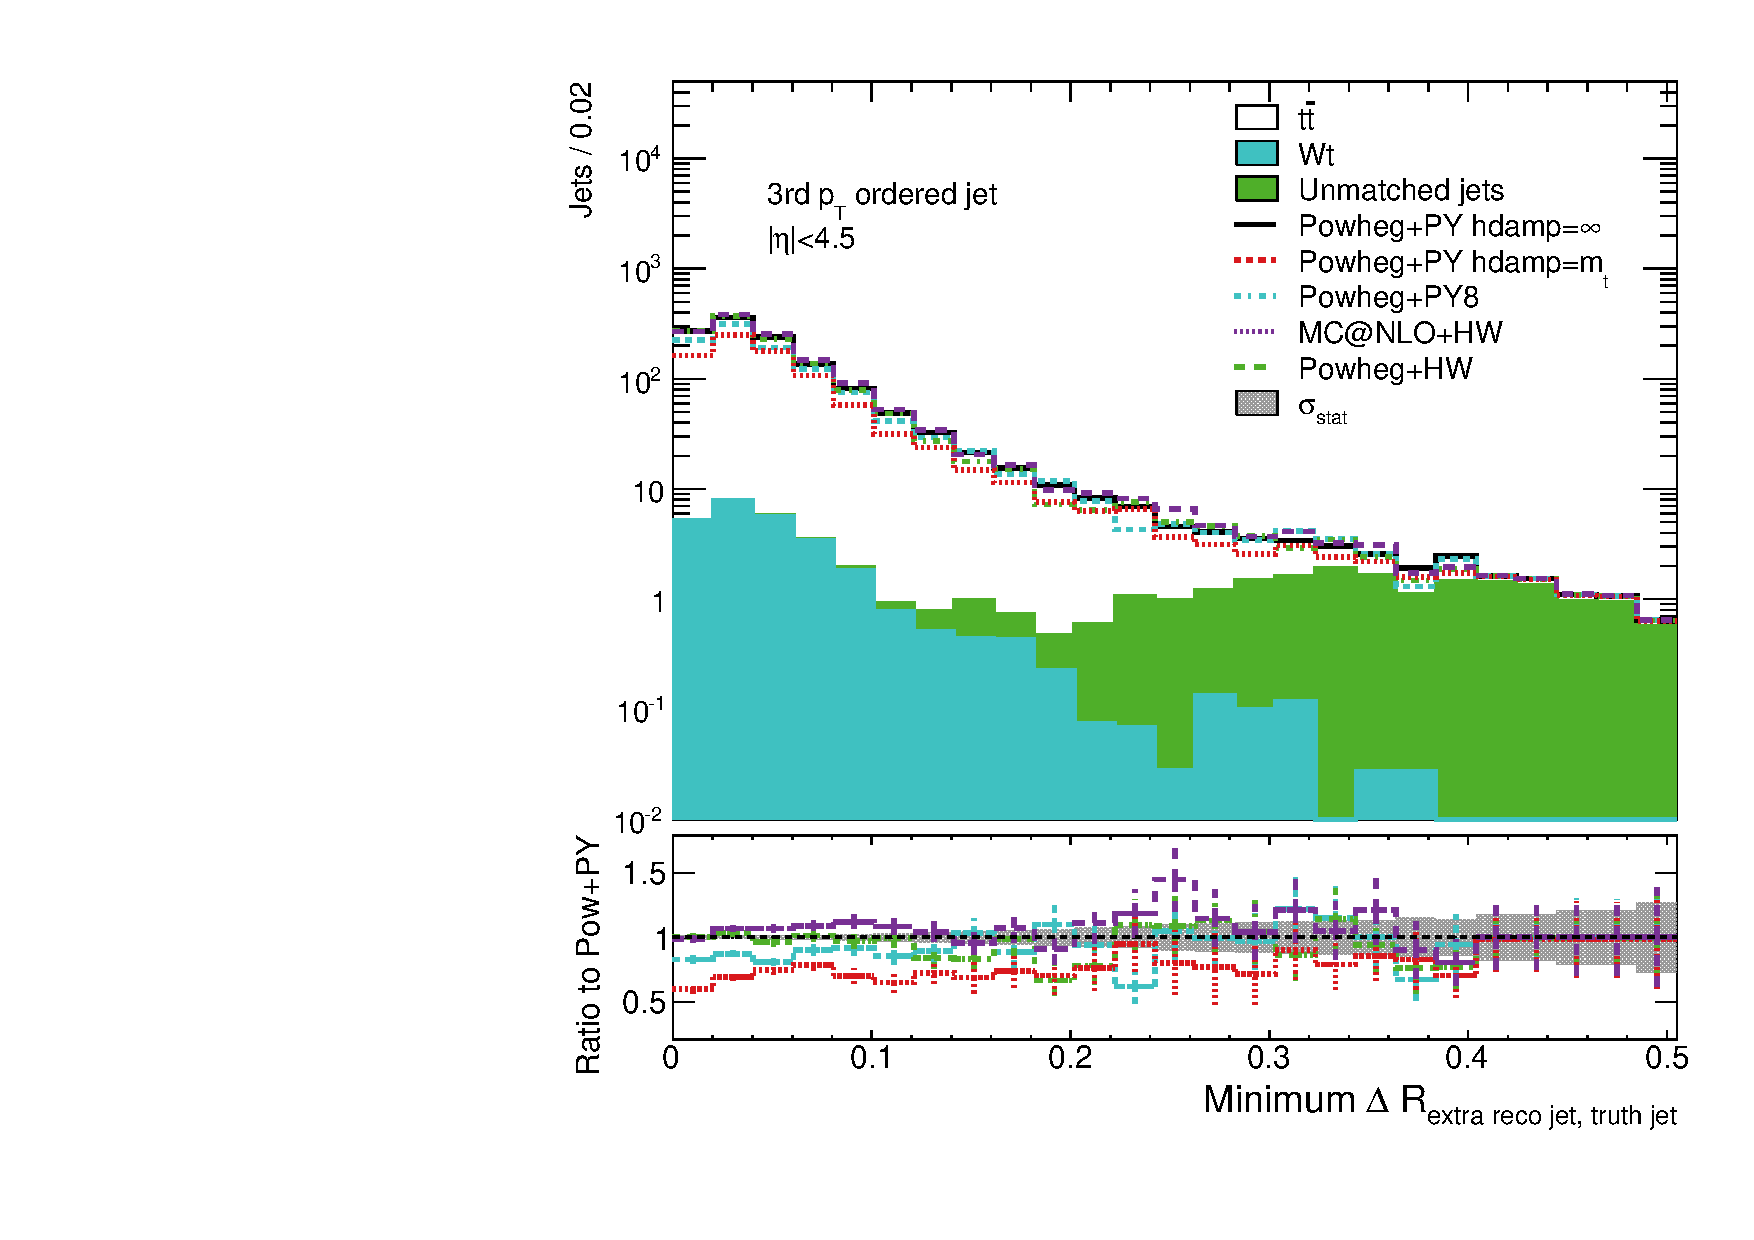
\includegraphics[width=\textwidth]{fig/MCComp/NLO/GrandPtVsTruthDRJet2.pdf}
\end{subfigure}
\begin{subfigure}[]{0.45\textwidth}
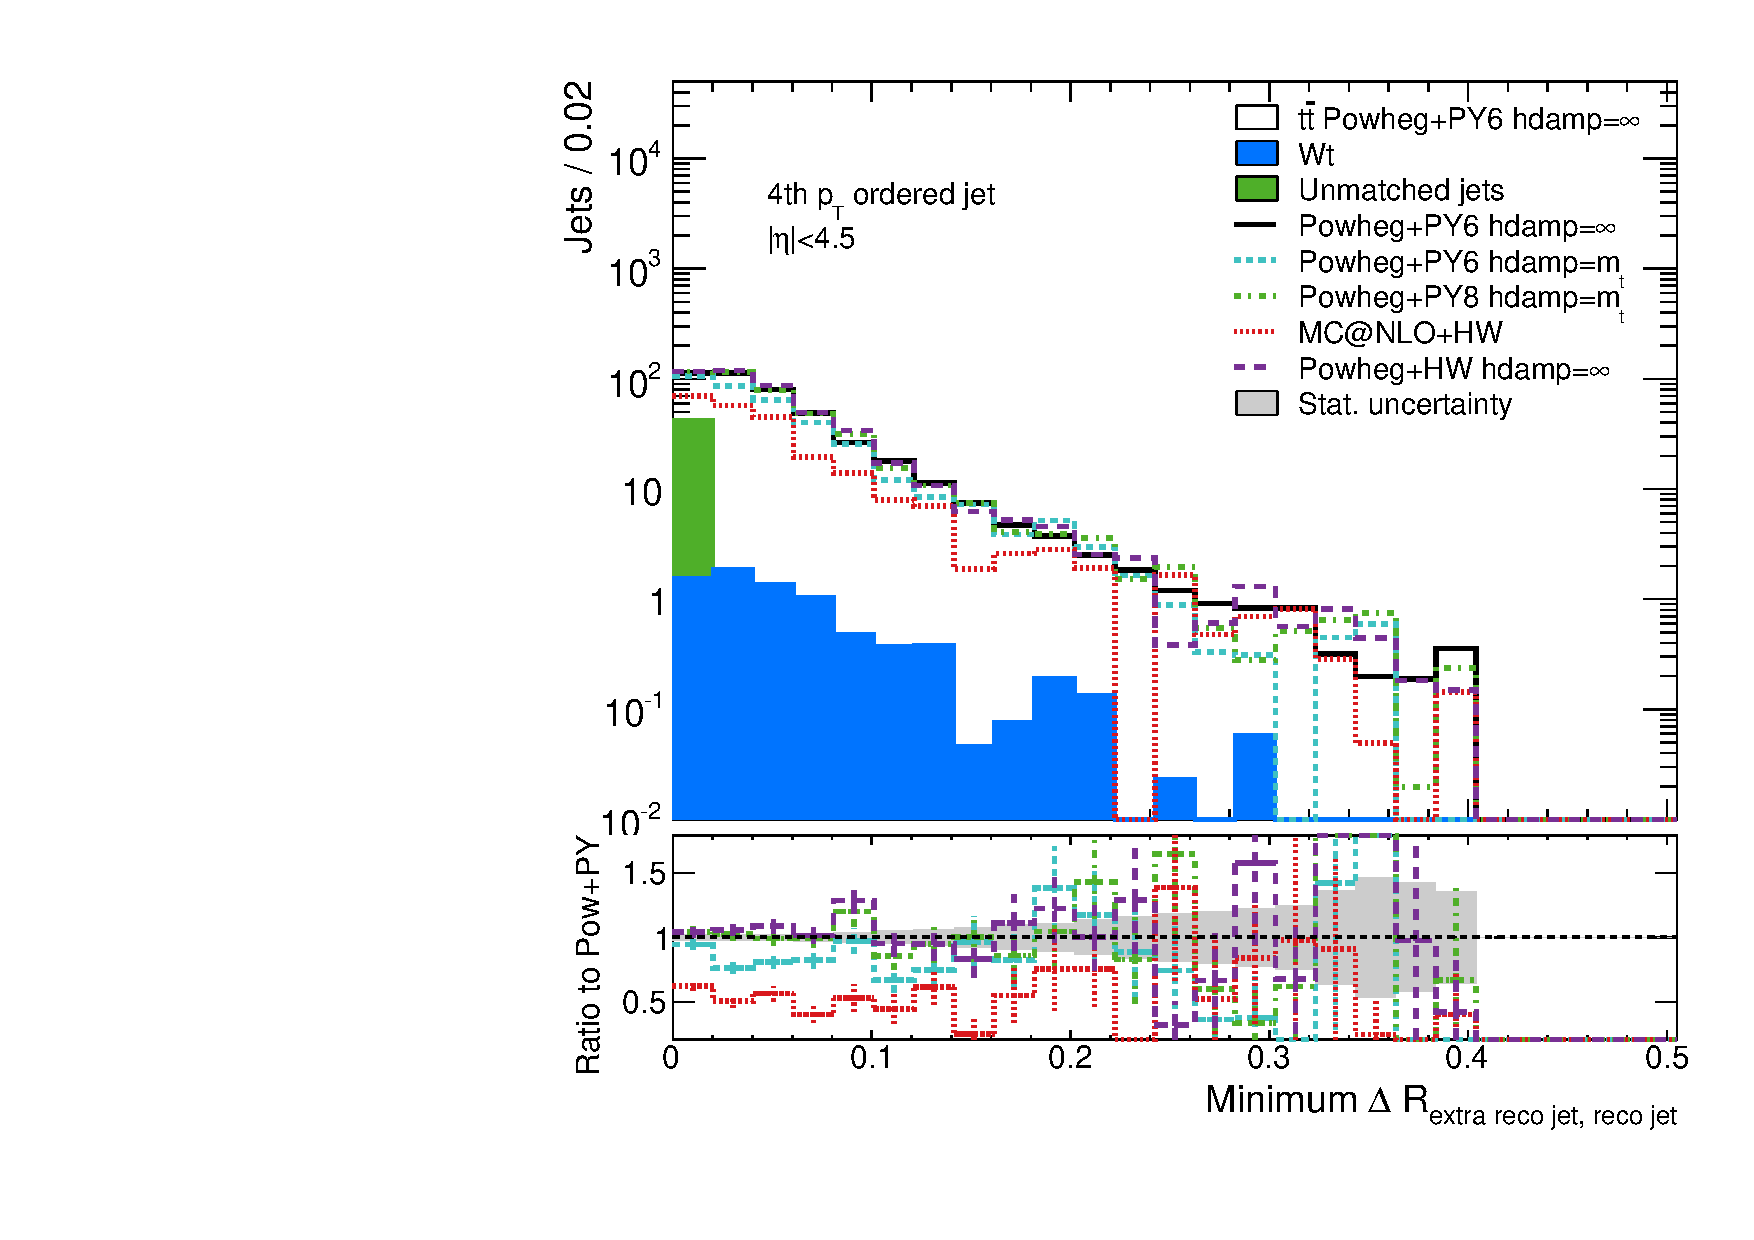
\includegraphics[width=\textwidth]{fig/MCComp/NLO/GrandPtVsTruthDRJet3.pdf}
\end{subfigure}
\caption{Distributions of $\Delta R$ betweeen reconstructed extra jets and the nearest truth jet for the first, second, third and fourth extra jet. }
\label{fig:truthdr}
\end{figure}
\section{Reconstruction level distributions}

Figures~\ref{fig:nrecojets} and~\ref{fig:recojetpt} compare the multiplicity and \pt of reconstructed extra jets in data and \ttbar simulation, where the simulation has been normalized to the number of events in data. Statistical uncertainity on the data is shown as a gray band on the ratio plot and statistical uncertainty on the simulation is shown as error bars on the ratio.  Systematic uncertainities are not shown. 
%For both the simulation and the data in Figure~\ref{fig:nrecojets}, jets from pileup are not included. 
%Pileup and false jet backgrounds have been removed from both the data and the simulation.
In data, background from pileup jets is subtracted, while in simulation, reconstructed jets are required to have a truth match. The multiplicity 
in the MC samples agree with that of the data, except for \mcnlohw, which consistently underestimates the number of events with 3 or more extra jets. Figure~\ref{fig:recojetpt} shows the \pt distributions of each extra jet, including contributions from single top events and unmatched jets. 
The fact that \mcnlohw\ underestimates the jet multiplicity can be seen in these distributions. The jets in \peight\ appear to exhibit a slightly harder spectrum than the data. All other generators agree reasonably well with the data. 
\begin{figure}
\centering
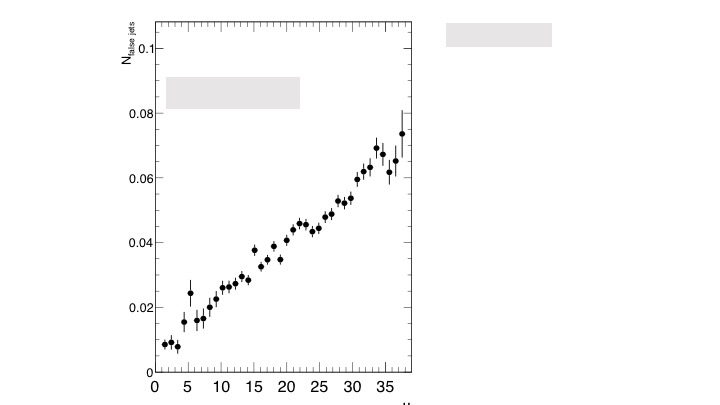
\includegraphics[width=0.9\textwidth]{fig/MCComp/FalseVsMuNoLbl.jpg}
\caption{Dependence of the unmatched extra jet rate on $\mu$ for the baseline simulation.}
\label{fig:falsecomp}
\end{figure}

\begin{figure}
\centering
\begin{subfigure}[]{0.45\textwidth}
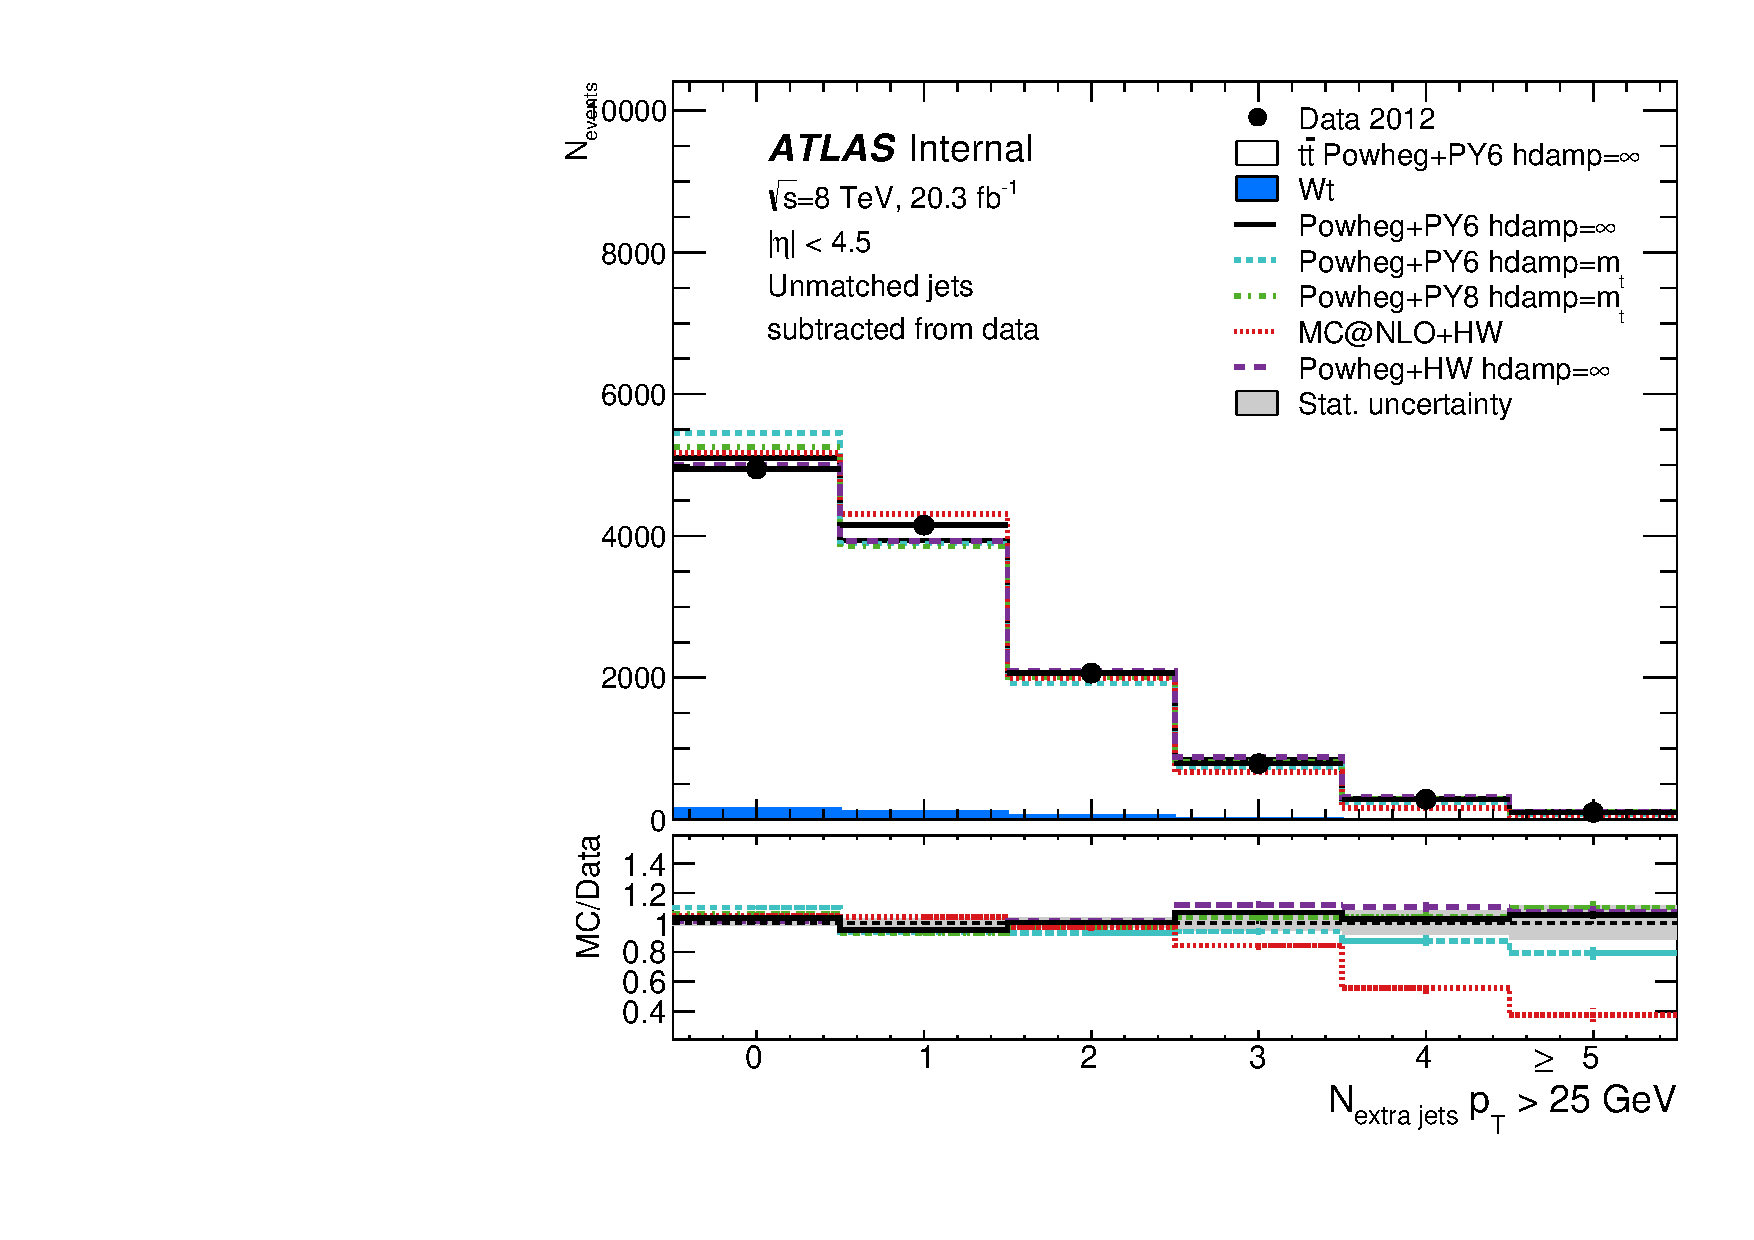
\includegraphics[width=\textwidth]{fig/MCComp/NLO/NExtraJets25NoPileup.pdf}
\end{subfigure}
\begin{subfigure}[]{0.45\textwidth}
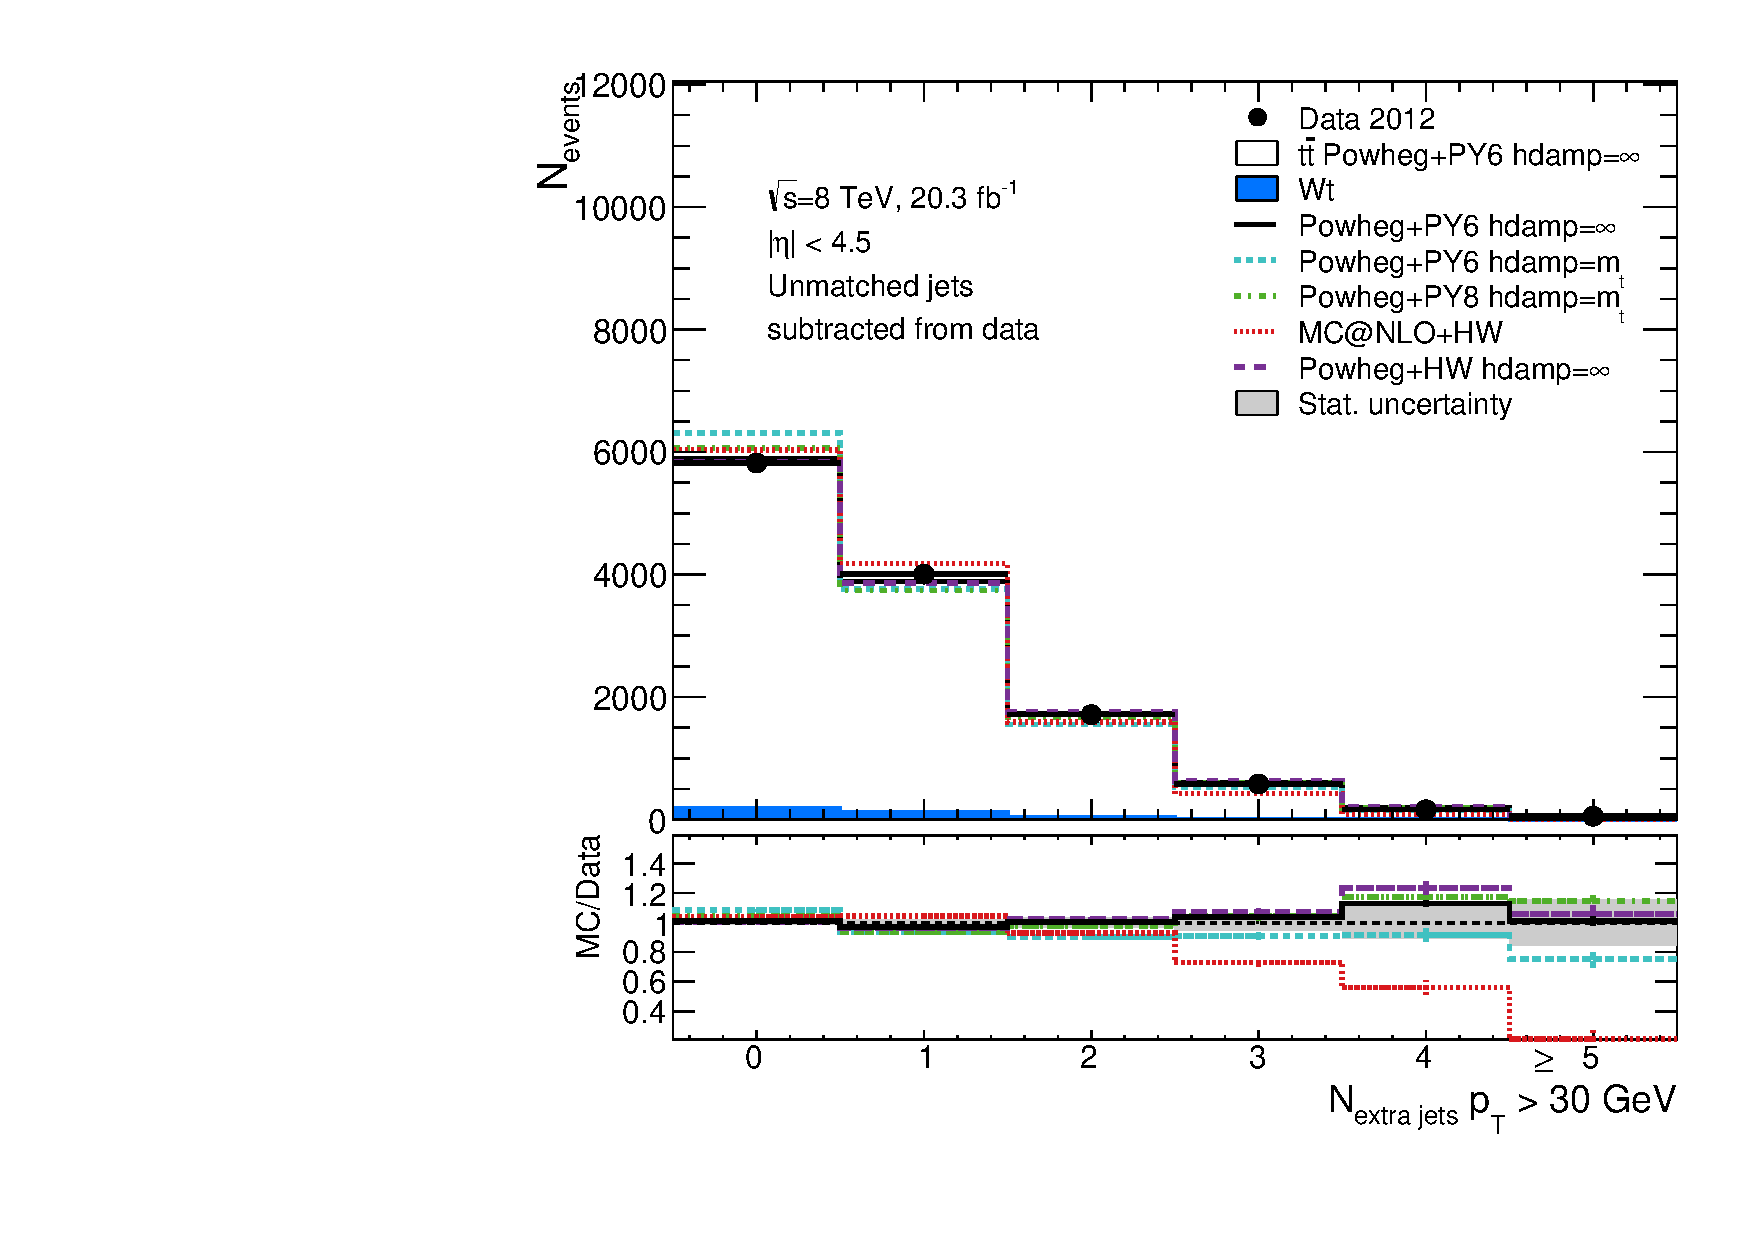
\includegraphics[width=\textwidth]{fig/MCComp/NLO/NExtraJets30NoPileup.pdf}
\end{subfigure}
\\
\begin{subfigure}[]{0.45\textwidth}
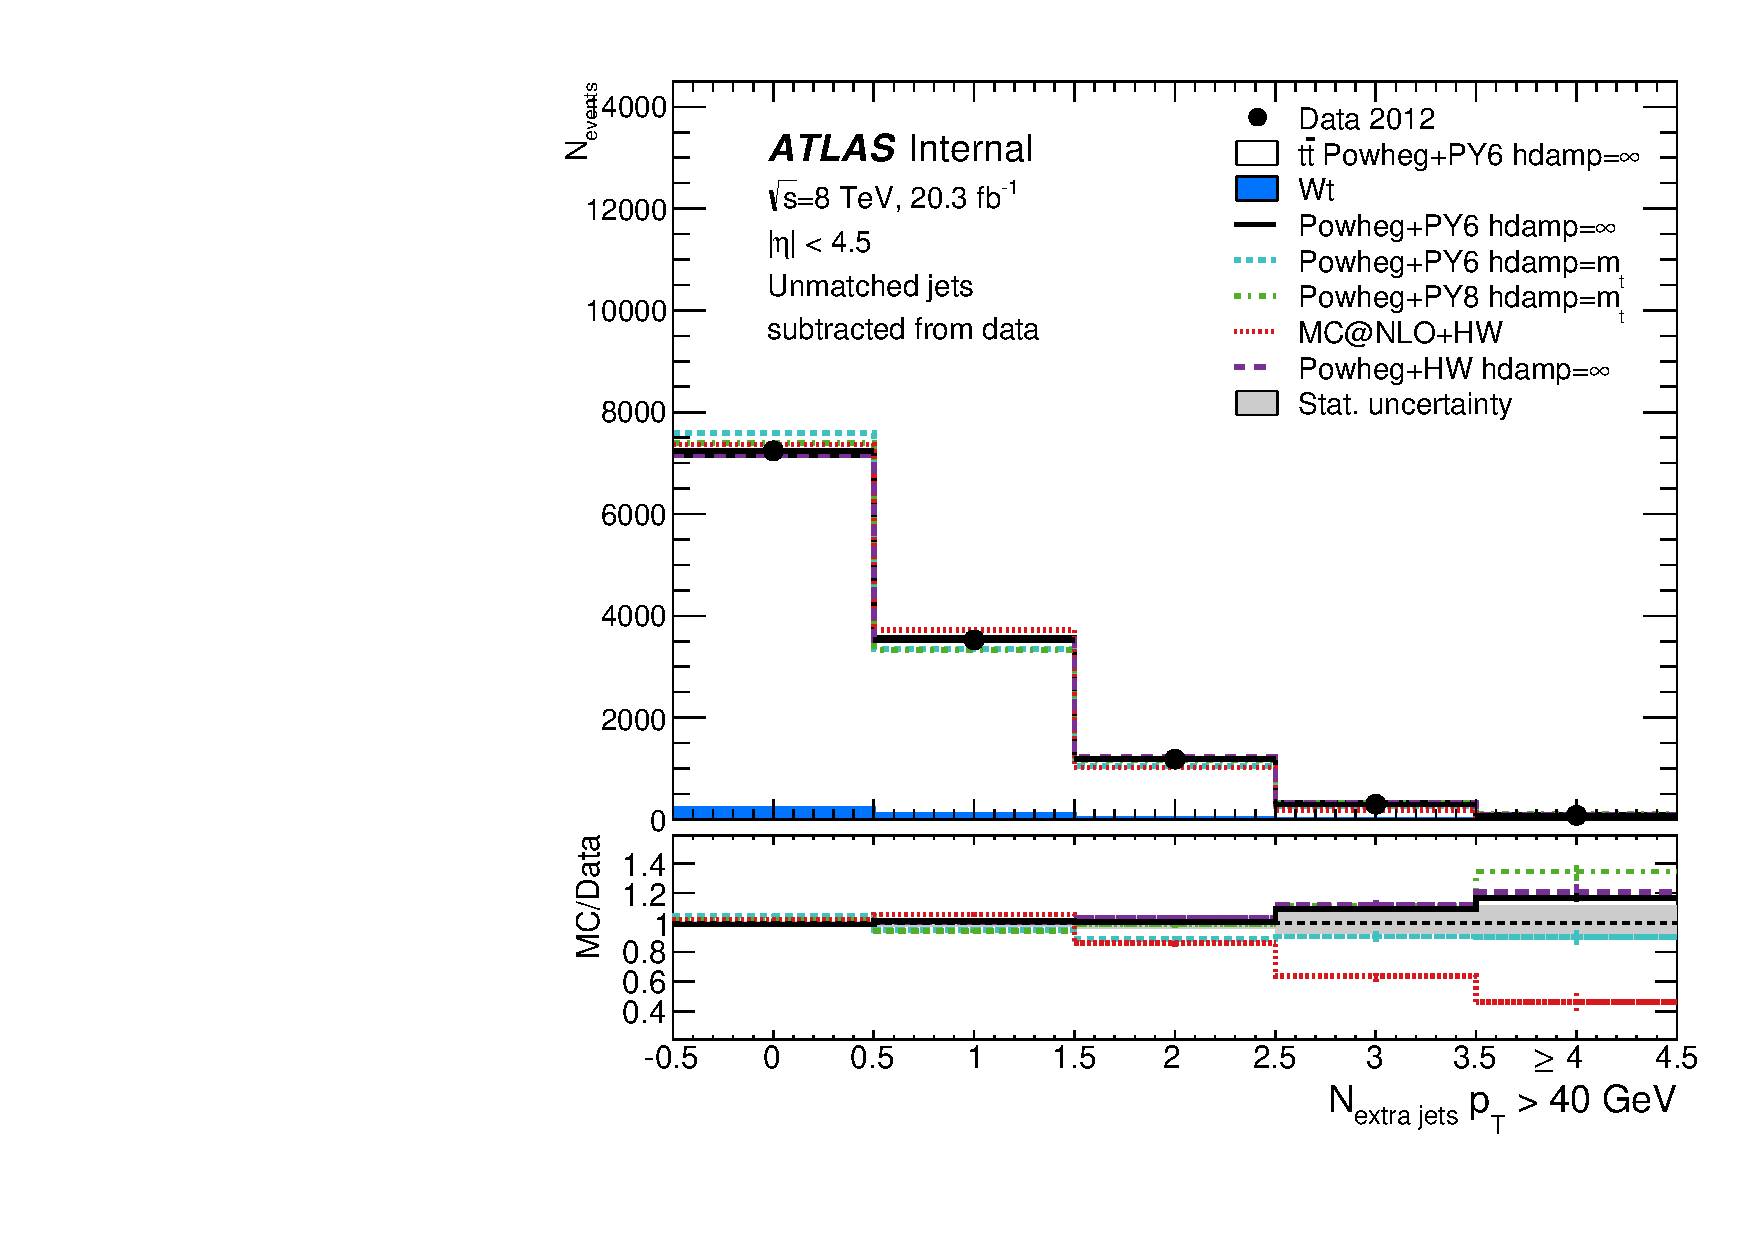
\includegraphics[width=\textwidth]{fig/MCComp/NLO/NExtraJets40NoPileup.pdf}
\end{subfigure}
\begin{subfigure}[]{0.45\textwidth}
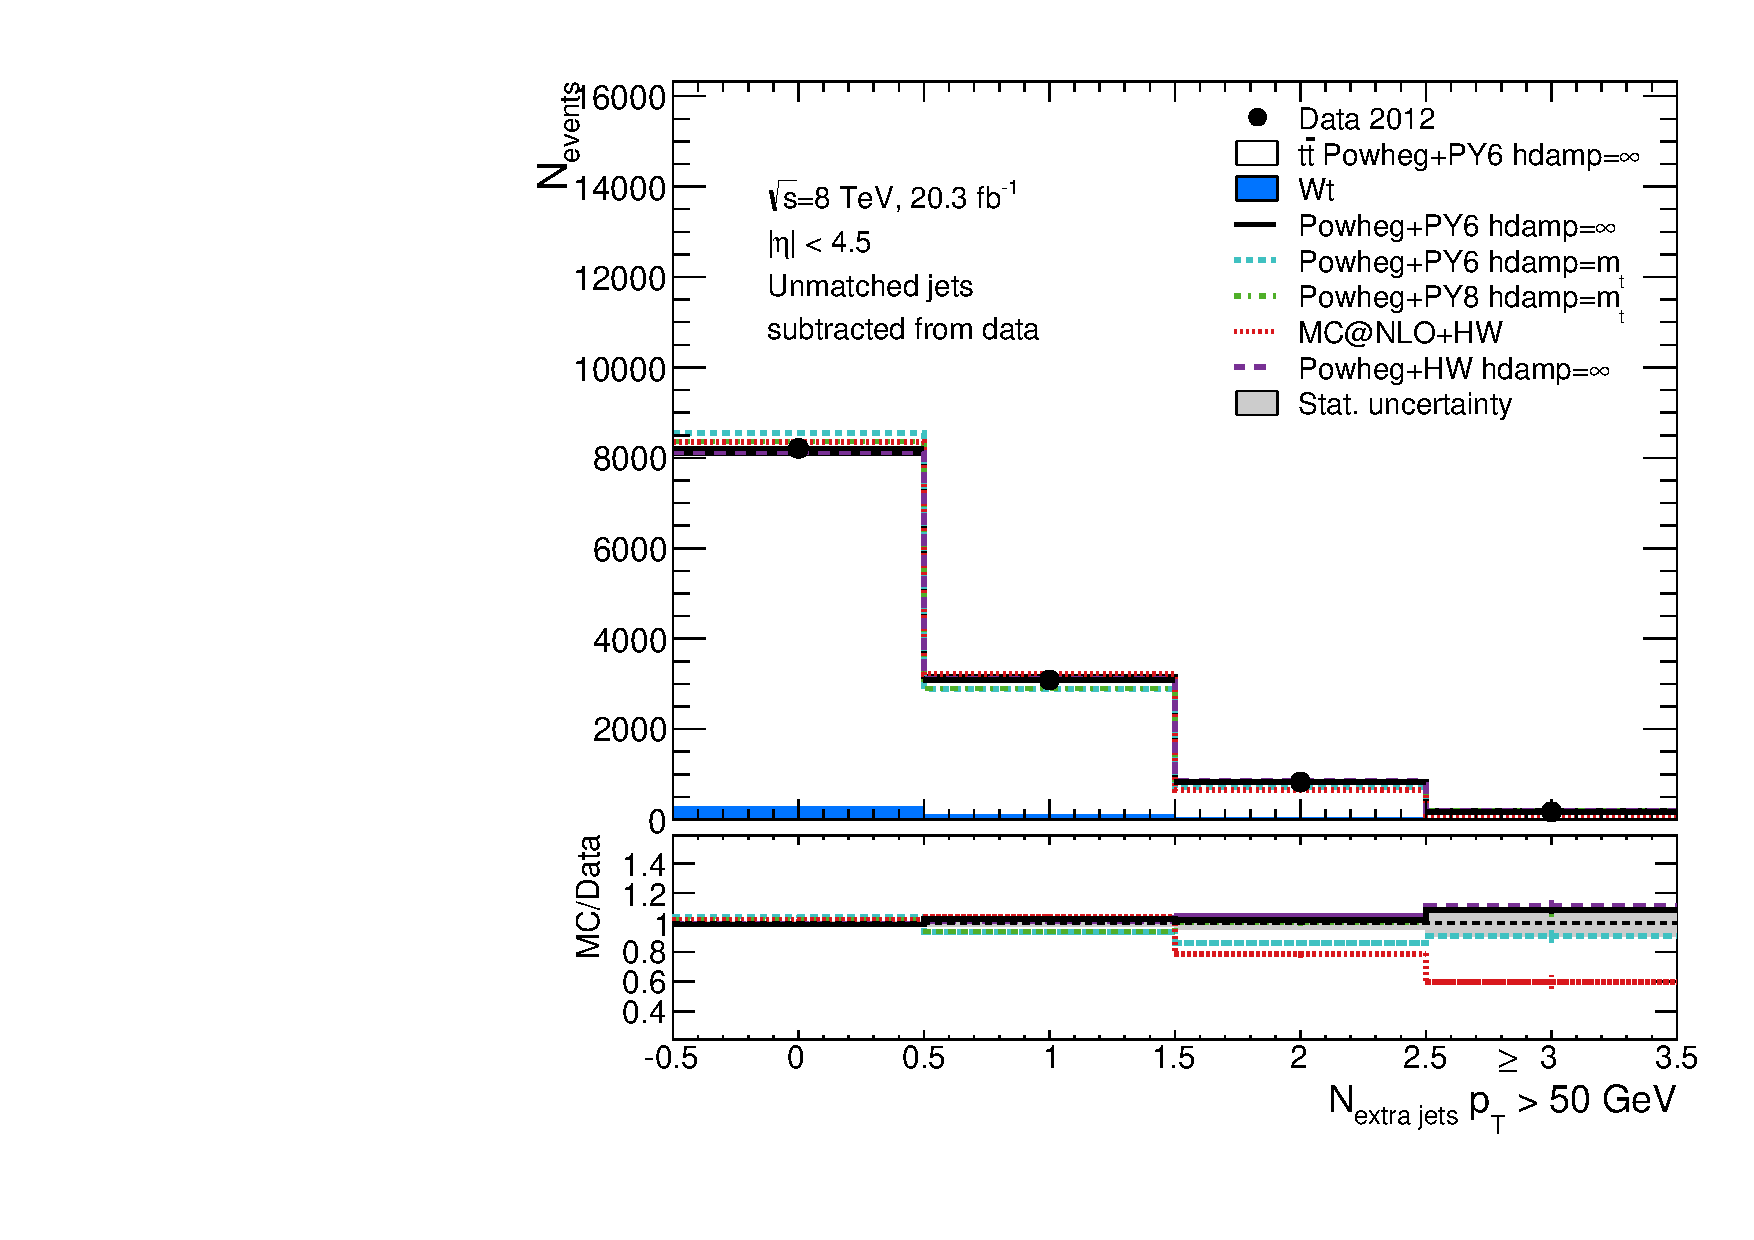
\includegraphics[width=\textwidth]{fig/MCComp/NLO/NExtraJets50NoPileup.pdf}
\end{subfigure}
\caption{Distributions of the reconstructed extra jet multiplicity as a function of \pt threshold in simulation and data. The distributions in data are compared to \ttbar simulation normalized to the same number of events as in the data. Extra jets from pileup are excluded in simulation by requiring a match to truth. Extra pileup jets are subtracted from the data. The ratio of different MC samples to data is shown with error bars corresponding to the MC statistical uncertainty and a shaded band corresponding to the data statistical uncertainty. Systematic uncertainities are not shown.}
\label{fig:nrecojets}
\end{figure}


\begin{figure}
\centering
\begin{subfigure}[]{0.45\textwidth}
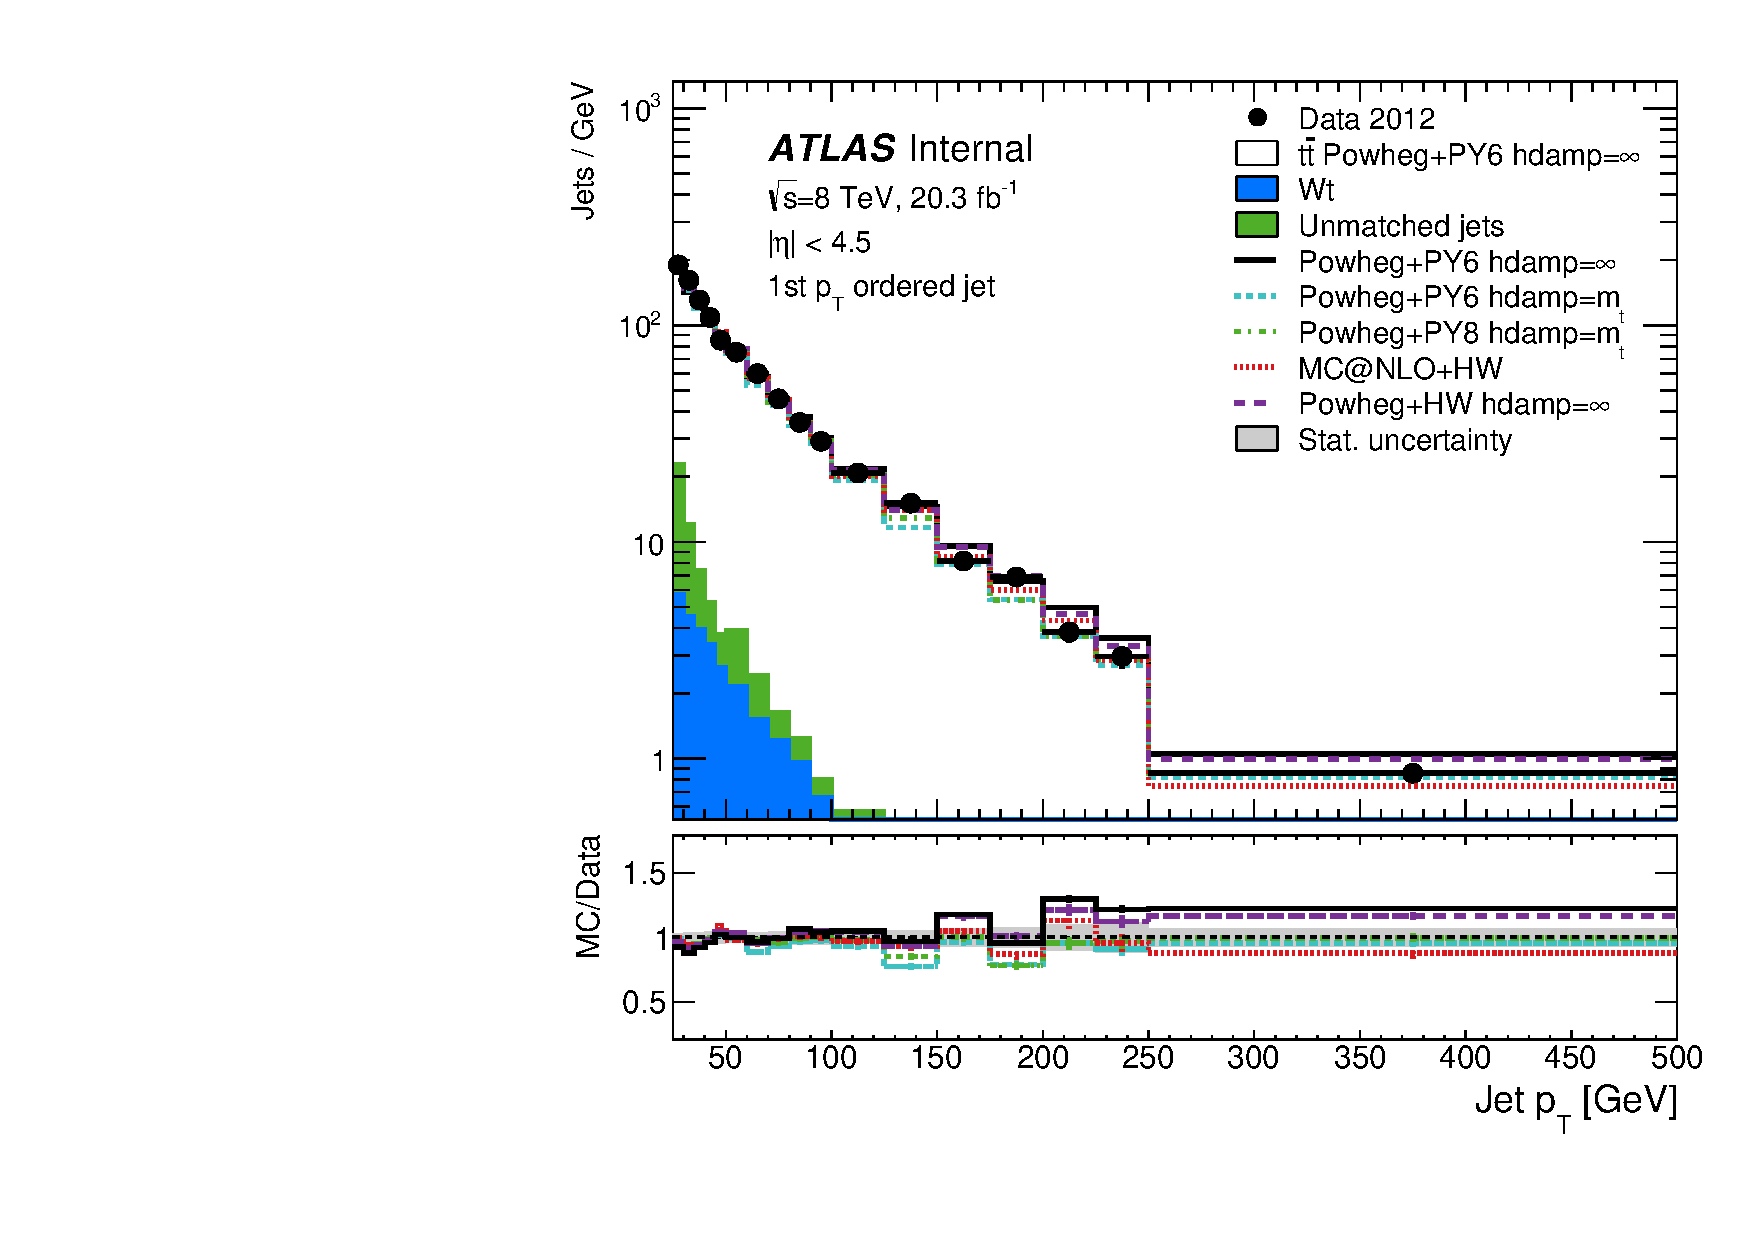
\includegraphics[width=\textwidth]{fig/MCComp/NLO/RecoPtJet0.pdf}
\end{subfigure}
\begin{subfigure}[]{0.45\textwidth}
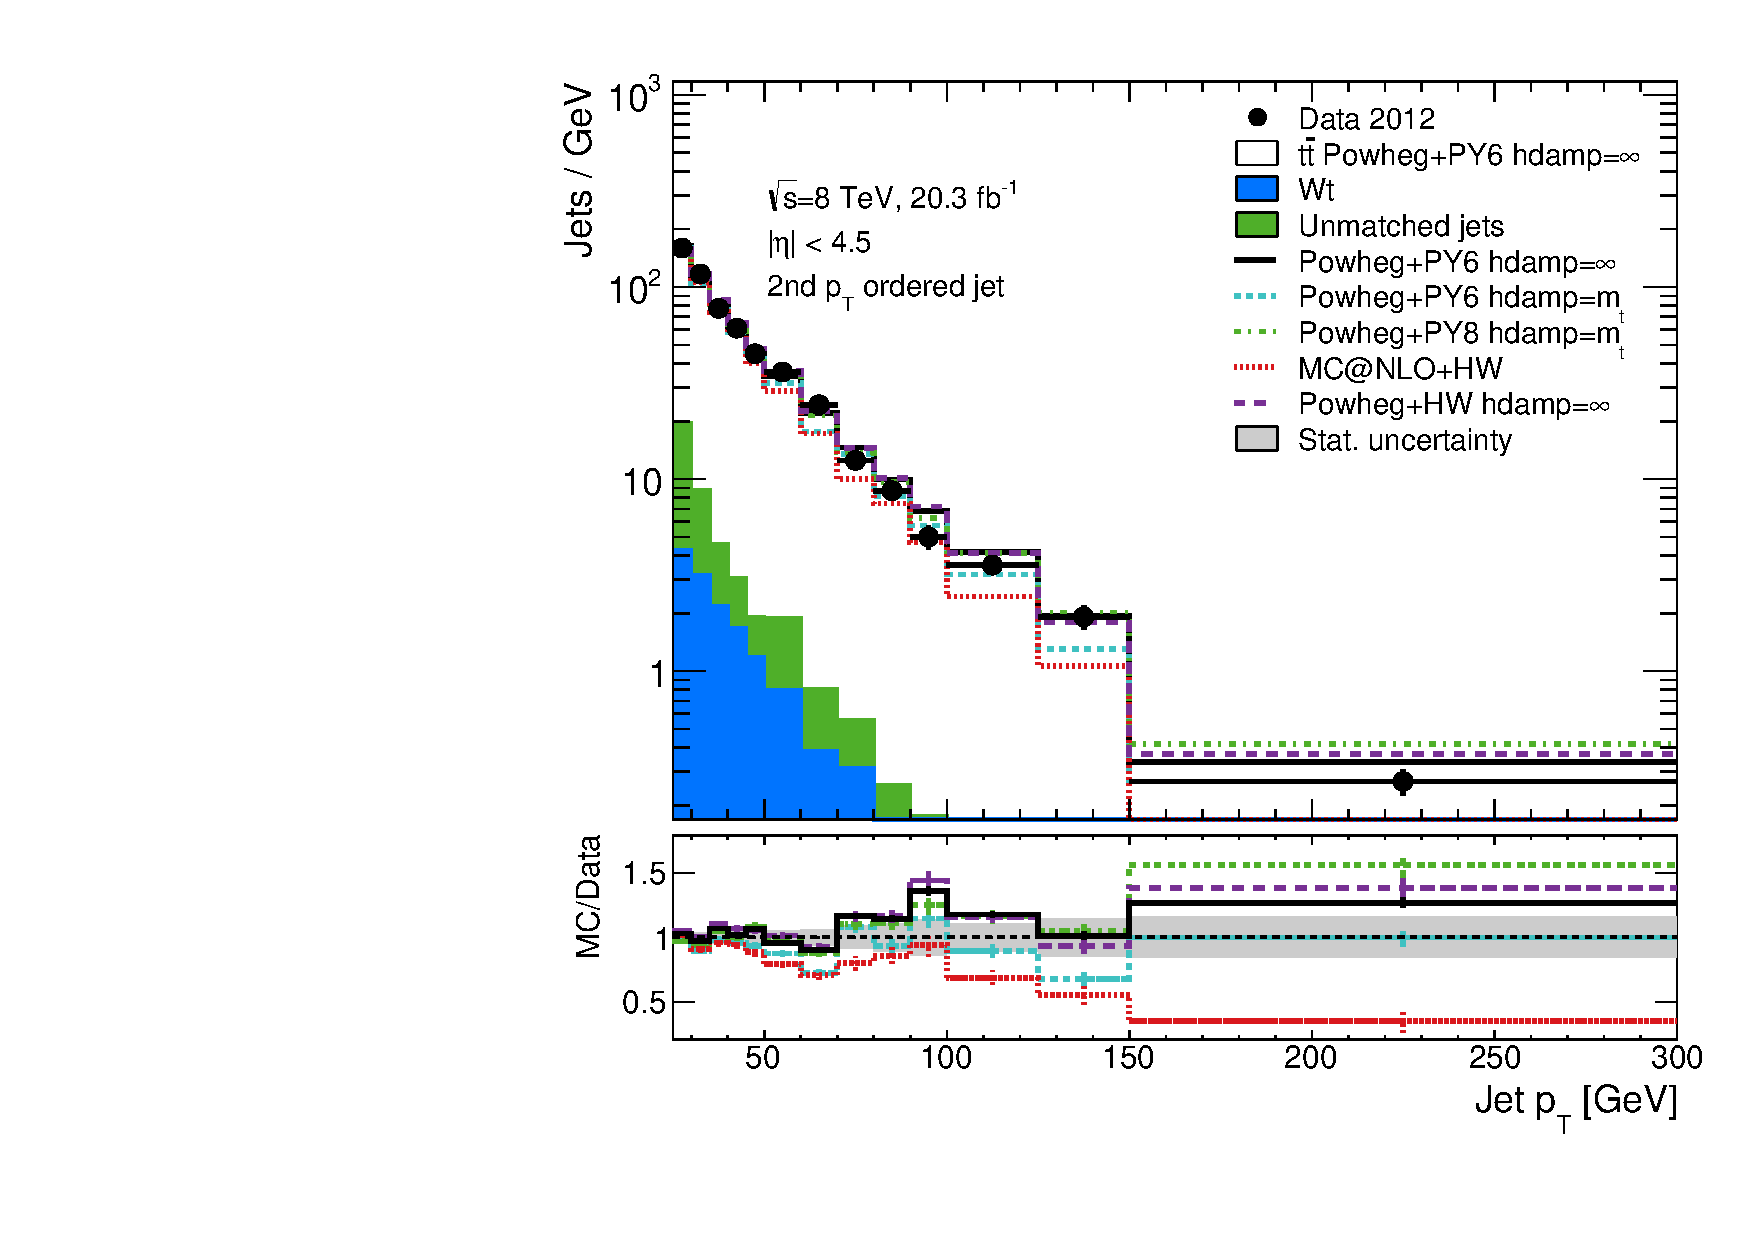
\includegraphics[width=\textwidth]{fig/MCComp/NLO/RecoPtJet1.pdf}
\end{subfigure}
\\
\begin{subfigure}[]{0.45\textwidth}
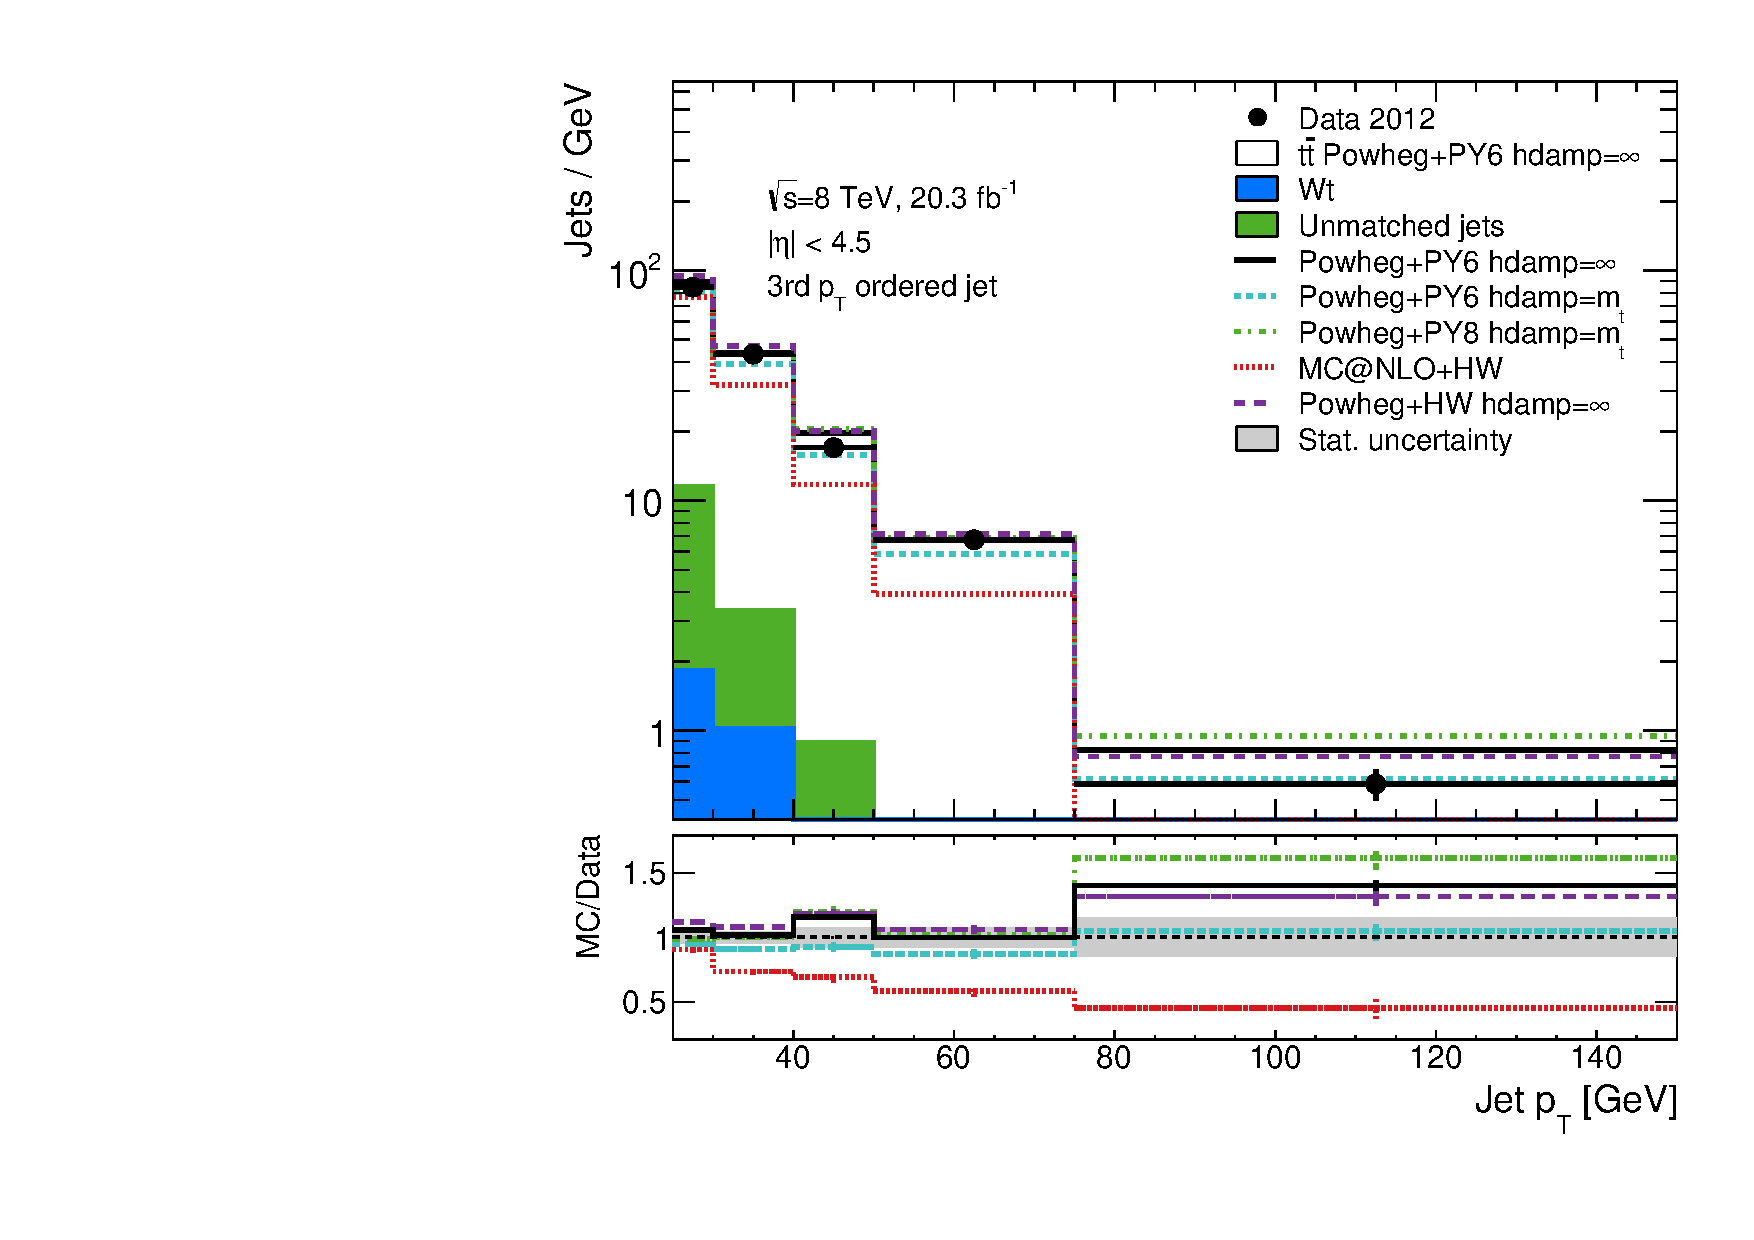
\includegraphics[width=\textwidth]{fig/MCComp/NLO/RecoPtJet2.pdf}
\end{subfigure}
\begin{subfigure}[]{0.45\textwidth}
\includegraphics[width=\textwidth]{fig/MCComp/NLO/RecoPtJet3.pdf}
\end{subfigure}
\caption{Distributions of reconstructed extra jet \pt in simulation and data. The distributions in data are compared to \ttbar simulation normalized to the same number of events as in the data. Backgrounds from single top and extra pileup jets are included as background to \ttbar. The ratio of different MC samples to data is shown with error bars corresponding to the MC statistical uncertainty and a shaded band corresponding to the data statistical uncertainty. Systematic uncertainities are not shown.}
\label{fig:recojetpt}
\end{figure}


\chapter{Correction to particle-level}
\label{ch:unfolding}
\section{Introduction to unfolding}
Kinematic distributions measured by a detector contain distortions due to limited acceptance, resolution and biases. The data must be corrected for these effects in order to allow direct comparison with theoretical models or other experimental measurements. This process of correcting the detector or reconstructed level back to the generator or truth level is called \emph{unfolding}.


Unfolding begins with building a \emph{response} (a.k.a. migration) matrix. The response matrix is a 2-dimensional representation of how the truth value of an observable relates to the measured value, as distorted by characteristic detector effects. The response matrix is built from simulated data.

In order to go from a reconstructed distribution to a truth distribution, the response matrix must be inverted. However, some bins of the matrix may be sparsely populated, and information loss occurs from detector imperfections. Directly inverting the matrix produces unphysical bin-to-bin fluctuations, so an unfolding uses \emph{regularization} to smooth the result and surpress these unphysical fluctuations. In this analysis, the iterative Bayesian algorithm is chosen, though the Singular Value Decomposition (SVD) technique was also considered.

\section{Procedure}
This section outlines the procedure used to unfold the reconstructed \pt and multiplicity of the 
extra jets using the software package \texttt{RooUnfold}~\cite{roounfold}.\footnote{Due to important bug fixes necessary for error propagation in this analysis, the development version of RooUnfold is used.}
This procedure corrects the background-subtracted measured spectrum to the true
spectum for events that pass the fiducial requirements at both the truth and the reconstruction level.
Detector effects can distort the true extra jet spectrum in several ways.  Hard scattering jets can be lost due to
inefficiencies in the reconstruction, resolution smearing will affect the jet \pt, and the rank of two
reconstructed jets can be swapped relative to the truth jets  (e.g. leading truth jet reconstructed as subleading jet or vice versa).
In addition, jets can migrate  into and out of the fiducial region.  The unfolding procedure corrects for all these effects.

The unfolding is performed on a distribution where the integral of the input distribution is the
number of measured jets in the sample and the integral of the output distribution is the number
of true jets passing the fiducial requirements. 

The full correction procedure is given by the equation:
\begin{equation}
\sigmapti = \frac{1}{N_{\textrm{events}}}\sum_j f^i \;\left ({\mathbf M}^{-1}\right )_{\textrm{reco,} j}^{\textrm{true, }i} g^j \left ({\mathscr N}^j_{\textrm {reco}}-
{\mathscr N}^j_{\textrm{bkgnd}} \right ) \ .
\label{eqn:unffinal}
\end{equation}
\noindent  ${\mathscr N}^j_{\textrm {reco}}$ gives the raw distribution measured from data. The estimated extra jet background, ${\mathscr N}^j_{\textrm{bkgd}}$ is subtracted from this raw distribution. 
A `feed-in' factor $g^j$ corrects for migration across the fiducial boundary (cases where the reconstructed jet has
$\pT>25$~GeV but the truth jet has $\pT>25$~GeV). The migration matrix ${\mathbf M}_{\textrm{reco, j}}^{\textrm{true, i}}$ 
relates the number of jets in truth bin $i$ to the number in reconstructed bin $j$. The correction factor $f^i$ 
removes the bias in the extra jet spectrum introduced by the event selection. Finally, the number of jets is normalized to the number of \emubb\ events passing the fiducial requirements ($N_{\textrm{events}}$) to obtain the final distribution.

This section is organized as follows.
First, the scheme for binning jets in both \pt\ and rank is discussed. 
Second, the method for the unfolding is outlined. Third, the correction factor for event selection is discussed.

\subsection{Binning}

In order to account for the migration effects described above in a single procedure, jets are binned according to both their \pt value and rank. 
For each jet rank, variable sized \pt\ bins are chosen to satisfy two criteria.
First, each bin must have at least 10 entries for the data. Second, each bin should show bias of less than 10\% of the statistical uncertainty in the closure test discussed in Chapter~\ref{ss:close}. In cases where the second criterion fails, neighboring bins are combined until the closure test passes this criterion. %Further studies showing the purity, stability, and \pt\ resolution for the binning can be found in Appendix~\ref{app:unfoldbin}.


The rank ($R$) and \pt\ of each jet in an event can be mapped to a single integer bin number ${\mathscr N}(\pt,R)$. 
The bin boudaries are given in Table~\ref{t:gbins}.  The last \pt\ bin for each rank is treated as an overflow bin.  %Rank $=5$ is defined to include all jets with rank $\ge 5$.

Both the \pt\ distribution and multiplicity of the extra jets can be recovered from the distribution ${\mathscr N}(\pt,R)$. 
The \pt\ distribution of the $R^{th}$ jet is obtained directly from ${\mathscr N}(\pt,R=k)$. 
The jet multiplicity can be obtained by integrating over $\pt$:
the number of events with at least $j$ jets with $\pt \geq p$ is given by:

\begin{equation}
N(\geq j) = \left\{
	\begin{array}{lr} 
	N_{\textrm{total}} & : j = 0 \\
	\int_{p}^{\infty} \! {\mathscr N}(\pt, R=j) \mathrm{d} \pt \, & : j > 0
	\end{array}
\right.
\label{eqn:inclmult}
\end{equation}

\noindent Then the number of events with exactly $j$ jets is given by:

\begin{equation}
N(j)=N(\geq j)-N(\geq j+1)
\label{eqn:exclmult}
\end{equation}

%\noindent This makes the table 
\noindent and the total number of jets with  exactly 0 jets is $N(0)=N_{total}-N(\geq 1)$, where $N_{total}$ is the total number of events.
\begin{center}
\begin{longtable}{|c|c|c|}
\caption{Binning for unfolding of extra jets. Jets are binned simultaneously in both rank (\pt order) and \pt. For each jet rank, variable sized \pt bins are chosen so that at least 10 data events fall in each bin. The first bin in \pt for each rank is treated as underflow bins. These bins are not reported as part of the measurement.} \label{t:gbins} \\ \hline
Bin number & Jet rank & Jet \pt (\GeV) \\
\hline 
\endfirsthead
\multicolumn{3}{l}%
 {\tablename\ \thetable\ --\textit{Continued from previous page}} \\ \hline
Jet rank & Bin number &  Jet \pt (\GeV) \\
\hline 
\endhead
\hline \multicolumn{3}{l} \textit{{Continued on next page}} \\
\endfoot
\hline \hline
\endlastfoot

\hline 
1 & 1 & $25-30$ \\ 
1 & 2 & $30-35$ \\ 
1 & 3 & $35-40$ \\ 
1 & 4 & $40-45$ \\ 
1 & 5 & $45-50$ \\ 
1 & 6 & $50-60$ \\ 
1 & 7 & $60-70$ \\ 
1 & 8 & $70-80$ \\ 
1 & 9 & $80-90$ \\ 
1 & 10 & $90-100$ \\ 
1 & 11 & $100-125$ \\ 
1 & 12 & $125-150$ \\ 
1 & 13 & $150-175$ \\ 
1 & 14 & $175-200$ \\ 
1 & 15 & $200-225$ \\ 
1 & 16 & $225-250$ \\ 
1 & 17 & $>250$ \\ 
\hline 
2 & 18 & $25-30$ \\ 
2 & 19 & $30-35$ \\ 
2 & 20 & $35-40$ \\ 
2 & 21 & $40-45$ \\ 
2 & 22 & $45-50$ \\ 
2 & 23 & $50-60$ \\ 
2 & 24 & $60-70$ \\ 
2 & 25 & $70-80$ \\ 
2 & 26 & $80-90$ \\ 
2 & 27 & $90-100$ \\ 
2 & 28 & $100-125$ \\ 
2 & 29 & $125-150$ \\ 
2 & 30 & $>150$ \\ 
\hline 
3 & 31 & $25-30$ \\ 
3 & 32 & $30-40$ \\ 
3 & 33 & $40-50$ \\ 
3 & 34 & $50-75$ \\ 
3 & 35 & $>75$ \\ 
\hline 
4 & 36 & $25-30$ \\ 
4 & 37 & $30-40$ \\ 
4 & 38 & $40-50$ \\ 
4 & 39 & $>50$ \\ 
\hline 
5 & 40 & $25-30$ \\ 
5 & 41 & $>30$ \\
\end{longtable}
\end{center}

\subsection{Unfolding procedure}
\label{ss:unfproc}
The unfolding algorithm corrects the number of jets reconstructed in each bin ${\mathscr N}^i_{\textrm {reco} }(\pt,R)$ for detector effects to obtain the unfolded ${\mathscr N}^i_{\textrm{unf} }(\pt,R)$ according to:

\begin{equation}
{\mathscr N}^i_{\textrm {unf}}= \sum_j \left ({\mathbf M}^{-1} \right )_{\textrm{reco,} j}^{\textrm{true,} i} g^j \left ({\mathscr N}^j_{\textrm {reco}}-{\mathscr N}^j_{\textrm{bkgd}}\right )
\label{eqn:unf}
\end{equation}

\noindent
The procedure begins with the raw ${\mathscr N}^j_{\textrm {reco}}$ distribution measured from data. 

First, the estimated extra jet background, ${\mathscr N}^j_{\textrm{bkgd}}$ is subtracted. This background is estimated from data and further discussed in Chapter~\ref{ss:pileup}. Sources of background  include jets from pileup and cases where
detector effects result in a single truth jet being split into 
two jets in the reconstruction. In simulation, background removal is done by requiring a match to a truth jet. 

Next, a factor $g$ corrects for migration across the fiducial boundary in reconstruction (cases where the reconstructed jet has
$\pT>25$~GeV but the truth jet has $\pT>25$~GeV). For each bin $j$, $g^j$ gives the fraction of reconstructed jets matched to truth jets inside the fiducial boundary ($>25 \gev$):
\begin{displaymath}
g^j \equiv \frac{{\mathscr N}^j_{\textrm {reco match }> 25 \gev}} {{\mathscr N}^j_{\textrm {all reco}}}
\label{eqn:feedin}
\end{displaymath}
Figure~\ref{fig:feedin} shows this factor estimated for several NLO \ttbar\ generators. The baseline \\
\powpy\ is used to correct the data.

The response matrix ${\mathbf M}_{\textrm{reco, j}}^{\textrm{true, i}}$ gives the number of jets reconstructed with bin number $j$; bin number $i$ is obtained from true \pt\ and rank.
The matrix is 
filled from simulated events that pass \textit{ both} reconstructed and truth selection requirements.
Figure~\ref{f:res} provides a graphical representation of ${\mathbf M}_{\textrm{reco, j}}^{\textrm{true}, i}$. 
The matrix is largely diagonal, showing that jets are most likely to be constructed with the correct \pt\ and rank.
However, there are significant numbers of truth subleading jets reconstructed as leading jets (for example ${\mathbf M}[1,18; 19,32]$), and 
truth leading jets reconstructed as subleading jets ( for example ${\mathbf M}[19,32;1,18]$). This type of migration motivates the simultaneous binning via both rank and \pt.



In RooUnfold, detector inefficiencies (cases where a true object is not reconstructed) are entered into the response matrix.  These
``misses'' are shown in Figure~\ref{f:res}(b) and are accounted for in the unfolding. 

The response matrix is inverted using iterative Bayesian unfolding~\cite{DAgostini:1994zf}, which reduces fluctuations from instabilities in 
the inversion process. The number of iterations has been set to 2. Details on the procedure used to determine the optimal number of iterations are described in Appendix~\ref{app:stressiter}. 
%This Appendix also shows the results of unfolding with alternate migration matrices. 
\begin{figure}
\includegraphics[width=0.45\textwidth]{fig/Unfolding/FeedIn.pdf}
\includegraphics[width=0.45\textwidth]{fig/Unfolding/FeedInFrac.pdf}
\caption{Fraction of reconstructed extra jets with truth matches inside the fiducial region (a) and ratio of alternate generators to the baseline (b). This factor is used to correct the data for \pt\ smearing across the fiducial boundary.}
\label{fig:feedin}
\end{figure}

\begin{figure}
\begin{subfigure}[]{0.45\textwidth}
\includegraphics[width=\textwidth]{fig/Cov/Response.pdf}
\end{subfigure}
~
\begin{subfigure}[]{0.45\textwidth}
\includegraphics[width=\textwidth]{fig/Cov/MissedPt.pdf}
\end{subfigure}
~
\caption{Migration matrix between the truth and reconstructed number of extra jets in each bin (a) and distribution of `missed' truth jets not matched to reco jets (b). Jets are binned according to both \pt value and rank. The matrix is filled from events passing both reconstructed and truth $e\mu$+2-$b$ jet events in the baseline \ttbar simulation. `Missed' jets are handled by the RooUnfold framework.}
\label{f:res}
\end{figure}
\subsection{Bias in extra jet distributions due to event selection requirements}
\label{sec:misid}
The unfolding procedure described above returns unbiased extra jet distributions for
events passing \textit{ both} the truth and reconstruction selection.  This subsample of events has
different kinematics from events passing the truth only selection.  Therefore, the extra jet
distributions obtained from the unfolding are biased with respect to the truth selection.
In addition, a secondary contribution to the bias results from events where one of the two reconstructed
$b$-jets is in fact a mistag.
Both of these biases are corrected using a single bin-by-bin correction factor that is applied after the unfolding. 

To understand the contributions to this correction, events that fall outside the combined truth and reconstructed
fiducial region are classified and their kinematic distributions are studied. 
These studies use the~\powpy~\ttbar\ baseline simulation. Table~\ref{t:truthrecoev} gives the number of events passing the fiducial selection for different combinations of reconstruction and truth selection.
Events passing both reconstructed and truth selection are properly handled by the unfolding and used to 
fill the migration matrix, but events that pass one set of selection criteria and not the other 
require additional corrections.  The subsections below provide additional information on each
failure category.

%COMMENT ABOUT MISMATCH OF EXTRA JETS INSIDE TRUTH+RECO EVENT???
\subsubsection{Reconstructed events that fail truth event selection}
Table~\ref{t:reconottruth} shows that $95.85\%$ of reconstructed $e\mu$+2 $b$-jet \ttbar\ events also pass the truth selection
and 4.15\%\ of these are \textit{misclassifed} events that fail. 
This table breaks these events into 5 categories:
%\begin{description}
\begin{enumerate}
\item{Lepton fiducial:} truth $e$ or $\mu$ fails the fiducial $p_{T}$ or $\eta$ cuts, while 
reconstructed $e$ or $\mu$ passes.
\item{Lepton jet overlap:}dressed truth $e$ or $\mu$  overlaps with a truth jet, while reconstructed $e$ or $\mu$ does not overlap with a reconstructed jet.
\item{Lepton non-prompt:} truth $e$ or $\mu$ leptons result from the decay of a hadron or are other background (such as
conversions).
\item{$b$-jet fiducial:} truth $b$-jet fails the fiducial $p_{T}$ or $\eta$ cuts.
\item{$b$-jet other:} truth jet not matched to $B$ hadron, meaning that the reconstructed $b$-jet was mistagged. 
This category also includes a small number of cases where the two reconstructed $b$-jets are matched to a single truth jet or 
one of the two reconstructed $b$-jets does match any truth jet.
\end{enumerate}
%\end{description}
Figure~\ref{fig:reconottruth} shows the electron \pt, $b$-jet \pt, $b$-jet MV1 weight, and extra jet multiplicity 
for events in the above categories. Additional plots of the kinematics and extra jets for these events can be found in Appendix~\ref{app:reconottruth}. 
Events failing the truth lepton or $b$-jet fiducial cuts arise mainly from resolution smearing of the \pt.
These produce a softer spectrum 
%as shown by the peak in the 25-30 \gev\ bin for 
for the reconstructed lepton \pt\ in Figure~\ref{fig:reconottruth}(a) and reconstructed $b$-jet \pt\ in Figure~\ref{fig:reconottruth}(b). 
Misclassified events with overlap between a lepton and a jet show a harder reconstructed lepton \pt\ spectrum and higher extra jet multiplicity, suggesting that a jet has been reconstructed from a lepton. Events with non-prompt leptons show similar properties. 
Finally, in the `$b$-jet other' category, the MV1 of the reconstructed $b$-jet is much lower than other types of events, 
suggesting that a light jet has been mistagged as a $b$-jet. The $\sim 1\%$ rate in this category is consistent with 
the mistag estimate for $b$-jets given in Ref.~\cite{btagmiscal}.

\subsubsection{Truth events that fail reconstructed event selection}
\label{ss:truthNotReco}
Due to detector inefficiencies, the majority of events passing the truth selection fail the reconstruction selection (\textit{missed events}). Table~\ref{t:truthnotreco} shows the events that pass truth selection broken into categories based on which objects were correctly reconstructed. The largest contributions come from failure to reconstruct the electron or the second $b$-jet in the event. A large fraction of these come from migrations across the fiducial boundary due to \pt\ smearing. 

Figure~\ref{fig:truthnotreco} shows the truth $b$-jet \pt, extra jet multiplicity, leading extra jet \pt\ and subleading extra 
jet \pt\ by category. Additional distribtuions can be found in Appendix~\ref{app:truthnotreco}. The $b$-jet \pt\ 
is much softer for events that are not reconstructed. The extra jets in these events are softer as well.

The differences in the extra jet distributions for these events can be explained by studying the relationship between the $b$-jet \pt\ 
and the number and kinematics of the extra jets. Figure~\ref{fig:bjetdep} shows the extra jet multiplicity and \pt\ in truth events in 
bins of $b$-jet \pt. Softer $b$-jets correspond to events with softer and fewer extra jets. This effect is likely the result of 
the dependence of the  $b$-jet \pt\ on \pttop. 

In summary, events that fail the reconstruction requirements on the $b$-jets have a lower extra jet multiplicity and 
softer jets than those that fall in other categories.   
%Although the extra jets in events that fail reconstruction differ significantly from those that pass, the difference can be understoood as a bias in \pttop. (TODO??) A systematic uncertainty on this difference can be set by varying \pttop .



\begin{table}
\begin{center}
\begin{tabular}{|l|c|}
\hline
Category & $N_{\textrm{events}}$\\
\hline
Reco & 11997.1 \\
Truth & 43496.9 \\
Reco AND truth & 11499.0 \\
Reco AND NOT truth & 498.2 \\
NOT Reco AND truth & 31877.7 \\
\hline
\end{tabular}
\end{center}
\caption{Number of events passing different combinations of truth and reconstructed selection requirements.}
\label{t:truthrecoev}
\end{table}

\begin{table}
\begin{center}
\begin{tabular}{|l|cc|}
\hline
Category & $N_{\textrm{events}}$ & (\%) \\
\hline
Lepton fiducial & 67.5 & 0.56 \\
Lepton jet overlap & 50.6 & 0.42 \\
Lepton non-prompt & 10.9 & 0.09 \\
$b$-jet fiducial & 245.8 & 2.05 \\
$b$-jet other & 123.4 & 1.03 \\
\hline
Total misclassified & 498.2 & 4.15 \\
\hline \hline
Passes reco and truth selection & 11499.0 & 95.85 \\
\hline
Total reco events & 11997.1 & 100.00 \\
\hline
\end{tabular}
\end{center}
\caption{Number of selected reconstructed events that fail truth selection categorized by reason they have failed.  The selections are applied sequentially in the order listed in the table.}
\label{t:reconottruth}
\end{table}

\begin{figure}
\centering
\begin{subfigure}[]{0.45\textwidth}
\includegraphics[width=\textwidth]{fig/RecoNotTruth/ElecPt.pdf}
\end{subfigure}
\begin{subfigure}[]{0.45\textwidth}
\includegraphics[width=\textwidth]{fig/RecoNotTruth/BJetPt.pdf}
\end{subfigure}
\\
\begin{subfigure}[]{0.45\textwidth}
\includegraphics[width=\textwidth]{fig/RecoNotTruth/BJetMV1.pdf}
\end{subfigure}
\begin{subfigure}[]{0.45\textwidth}
\includegraphics[width=\textwidth]{fig/RecoNotTruth/NJets.pdf}
\end{subfigure}
\caption{Distributions of the (a) $e$ \pt, (b) $b$-jet \pt, (c) $b$-jet MV1 weight and (d) extra jet multiplicity. Each distribution is normalized by the number of events falling in that category. Events were simulated with \powpy~\ttbar.}
\label{fig:reconottruth}
\end{figure}


\begin{table}
\begin{center}
\begin{tabular}{|l|cc|}
\hline
Category & $N_{\textrm{events}}$ & (\%) \\
\hline
No $e$ & 13472.3 &	31.06 \\
No $\mu$ & 3743.0 & 8.63 \\
same-sign $e\mu$ & 161.1 & 0.37 \\
0 $b$-jets & 2986.0	& 6.88 \\
1 $b$-jet  & 11515.3 & 26.55 \\
\hline
Missed total & 31877.7 & 73.49 \\
\hline \hline
Passes reco and truth selection & 11499.0 & 26.51 \\
\hline
Total truth events & 43376.7 & 100.00 \\
\hline

\end{tabular}
\caption{Number of truth events that fail reconstruction selection categorized by reason they have failed. The selections are applied sequentially in the order listed in the table.}
\label{t:truthnotreco}
\end{center}
\end{table}

\begin{figure}
\centering
\begin{subfigure}[]{0.45\textwidth}
\includegraphics[width=\textwidth]{fig/TruthNotReco/TruthBJetPt.pdf}
\end{subfigure}
\begin{subfigure}[]{0.45\textwidth}
\includegraphics[width=\textwidth]{fig/TruthNotReco/NTruthExtraJets30.pdf}
\end{subfigure}
\\
\begin{subfigure}[]{0.45\textwidth}
\includegraphics[width=\textwidth]{fig/TruthNotReco/TruthPtJet0.pdf}
\end{subfigure}
\begin{subfigure}[]{0.45\textwidth}
\includegraphics[width=\textwidth]{fig/TruthNotReco/TruthPtJet1.pdf}
\end{subfigure}
\caption{Distributions of the truth (a) $b-$jet \pt, (b) extra jet multiplicity, (c) leading extra jet \pt and (d) subleading extra jet \pt. Each distribution is normalized by the number of events falling in that category. Events were simulated with \powpy~\ttbar and required to pass the fiducial truth $e\mu$+2 $b$-jet selection.}
\label{fig:truthnotreco}
\end{figure}

\begin{figure}
\centering
\begin{subfigure}[]{0.45\textwidth}
\includegraphics[width=\textwidth]{fig/TruthNotReco/BJetNJets30.pdf}
\end{subfigure}
\begin{subfigure}[]{0.45\textwidth}
\includegraphics[width=\textwidth]{fig/TruthNotReco/BJetPtJet0.pdf}
\end{subfigure}
\\
\begin{subfigure}[]{0.45\textwidth}
\includegraphics[width=\textwidth]{fig/TruthNotReco/BJetPtJet1.pdf}
\end{subfigure}
\begin{subfigure}[]{0.45\textwidth}
\includegraphics[width=\textwidth]{fig/TruthNotReco/BJetPtJet2.pdf}
\end{subfigure}
\caption{Distributions of the truth (a) extra jet multiplicity, (b) leading extra jet \pt, (c) subleading extra jet \pt and (d) subsubleading extra jet \pt in bins of the average of the \pt of the two truth $b$-jets used to select the event. Each distribution is normalized by 
the number of events falling in that bin. Events were simulated with \powpy~\ttbar and required to pass the fiducial truth $e\mu$+2 $b$-jet selection.}
\label{fig:bjetdep}
\end{figure}


\subsubsection{Event selection correction factors}
\label{ss:unfcorr}

To correct for the effects discussed above, bin-by-bin correction factors $f^i$ are applied to the 
unfolded distribution as shown in Equation~\ref{eqn:unffinal}. These factors are derived by 
comparing unfolded simulated events that pass the reconstruction selection (with no particle level event selection) to
particle level truth distributions where no reconstruction requirements are applied.
Each bin's correction factor is given by:
\begin{equation}
f^i \equiv \frac{{\mathscr N}^i_{\textrm{true}}} {{\mathscr N}^i_{\textrm{unf}}}
\label{eqn:corrf}
\end{equation}
The simulated data used for this study includes \ttbar\ and single top events with their relative contributions determined
from their NLO cross sections. ${\mathscr N}^i_{\textrm{true}}$ and ${\mathscr N}^i_{\textrm{unf}}$ are normalized by number of events passing \emubb\ selection at the reconstructed and particle level, respectively. Since the final measurement given by Equation~\ref{eqn:unffinal} is normalized by the number of events in data, the correction factor $f^i$ corrects only for the bias in the extra jet spectrum, not the efficiency in number of events.
Figure~\ref{fig:bincorr} shows the correction factors obtained using different choices of generator for the \ttbar\ component.
The final correction factors used for data are taken from the baseline \powpy\ sample. Systematic uncertainties associated with generator dependence of this factor are discussed in Chapter~\ref{ss:unfsystt}.


% with the average difference 
%between \powpy\ and the other two generators as the systematic uncertainty. 
%The values of the correction factors are presented in Table~\ref{t:tcorr} in Appendix~\ref{app:tcorr}.



\begin{center}
\begin{figure}
\begin{subfigure}[]{0.45\textwidth}
\includegraphics[width=\textwidth]{fig/Unfolding/CorrFactors.pdf}
\end{subfigure}
~
\begin{subfigure}[]{0.45\textwidth}
\includegraphics[width=\textwidth]{fig/Unfolding/RatioCorrection.pdf}
\end{subfigure}
\caption{(a) Ratio of unfolded extra jets to truth extra jets different \ttbar generators (including a 2.9\% contribution from single top). (b) Fractional difference of the correction factorfrom baseline for different generators. Extra jets in events passing reconstructed and truth selection for each generator are added to single top and used to fill a response matrix. Then each generator is unfolded against itself, using all selected reconstructed events. Extra jet truth distributions are made without any reconstruction requirements. Finally, the unfolded distribution is divided by the truth distribution to obtain a correction factor for each bin.
\label{fig:bincorr}}
\end{figure}
\end{center}




\section{Validation}
%%COVARIANCE DISCUSSION HERE

\texttt{ RooUnfold} allows propagation of the full covariance matrix of the measured distribution through the unfolding. 
The package returns a covariance matrix, which is used to determine the uncertainties
on the unfolded spectrum. %and an inverse covariance matrix, which is used to calculated the $\chi^2$ betweenthe unfolded data and a predicted truth spectrum including correlations.
The covariance matrix $X$ on the unfolded distribution is calculated via pseudoexperiments. The diagonal elements of this covariance matrix give the uncertainties on the bins of \pt\ and rank. 

% The inverse of the covariance matrix is needed to compute the \chisq\ agreement between the unfolded and truth distributions. However, the regularized covariance matrix $X^{\tau}$ is singular and cannot be inverted. 
% Therefore, using and appropriate change of variable, the non-regularized inverse covariance matrix from the unfolding 
% ($X^{-1}$) can be used to compare true and unfolded distributions (see Eq. 53 in Ref.~\cite{svd}). This subtle distinction is discussed in more explicit detail in Ref.~\cite{svdphystat}.

The agreement between an unfolded spectrum and truth distribution can be estimated using a $\chi^2$ test (including correlations among bins):
\begin{equation}
\chi^2= \left( {\mathscr N}_{\textrm {unf}}- {\mathscr N}_{\textrm {true}} \right)^{T} X^{-1}\left( {\mathscr N}_{\textrm {unf}}- {\mathscr N}_{\textrm {true}} \right)
\label{eq:unfchi2}
\end{equation}
 The inverse covariance matrix, $X^{-1}$, is determined using Singular Value Decomposition (SVD) with \texttt{ SciPy}~\cite{scipy}.

This \chisq\ is used validate the unfolding procedure with different MC generators in Chapter~\ref{ss:close}-\ref{ss:stress}, as well as to assess the agreement of generators with the fully corrected data in Chapter~\ref{ch:results}.
\subsection{Closure test}
\label{ss:close}
The closure test validates the unfolding procedure using simulation. The stability of unfolding can depend on the statistical power of the input data. To ensure that the the closure test appropriately accounts for this effect, the test is performed using pseudoexperiments with the same statistical power as the data.

In the closure test, the baseline \ttbar+3\% $Wt$ simulation is used to fill the migration matrix and
one thousand pseudoexperiments are performed using randomly chosen subsamples of events.  Each pseudoexperiment is chosen
so the number of events is equal to that of data. 
The extra jet distribution from each pseudoexperiment is then unfolded.  Each unfolded distribution is 
compared to the truth distribution obtained from the full sample of events used to train the migration matrix. 

The bias $B^i={\mathscr N}^i_{\textrm{ truth}}-{\mathscr N}^i_{\textrm{unfold}}$ and 
pull $P^i=({\mathscr N}^i_{\textrm{truth}}-{\mathscr N}^i_{\textrm{unfold}})/\sigma_{\textrm {unfold}}$ 
distributions are measured for each bin $i$. 
Figure~\ref{fig:UnfoldPull} shows the mean pull and its uncertainty in bins of \pT\ for jets of rank~1 through~5.  The shaded bands indicate
the width of the pull distribution, obtained from a Gaussian fit.
The pull distributions for each bin are shown in Appendix~\ref{app:unfoldpull}. 
The mean pull is close to zero and has a width close to unity.  This demonstrates that the unfolding procedure has no 
significant bias and that the statistical uncertaintainties on the unfolded distribution are properly estimated. Additional test of the unfolding are provided in Appendix~\ref{app:unfoldval}. 

In addition to the pull and bias, the average \chisq\ between the unfolded pseudoexperiments and the true distribution is computed using Equation~\ref{eq:unfchi2}.  The \chisq\ obtained in the closure test is 42 for 41 degrees, indicating that the
inverse covariance matrix returned from RooUnfold appropriately estimates the correlated uncertainties. 

\subsection{Stress test}
\label{ss:stress}
`Stress' tests assess the effect of the input \pt\ spectrum on the unfolding algorithm by unfolding pseudoexperiments produced from alternate \ttbar\~MC generators (described in Chapter ~\ref{ss:mcsignal}) using the response matrix and correction factors
obtained from the baseline. 

To study the stability of the unfolding with respect to changes in the input jet \pt\ and multiplicity spectra, pseudoexperiments are constructed by reweighting the truth jet spectrum in the baseline MC sample. The weight for each bin is given by the ratio of the alternative generator to the baseline\footnote{An alternative reweighting procedure where the ratios were fit to a smooth function was also studied. Changes with respect to the procedure described here were small}. This procedure isolates the uncertainty associated with the choice of spectrum from other generator-independent sources of instability (e.g. JES), which are accounted for separately. %ADD MORE EXPLANATION??

Stress tests have been performed using the following samples: \pow+\py, \pow+\hw, \madpy, \mcnlohw, \peight, \hdamp, RadHi \madpy\ and RadLo \madpy. Each of the alternate \ttbar\ samples are unfolded with 1000 pseudoexperiments against a migration matrix filled from the baseline \ttbar\ simulation. In both the migration matrix and the samples, a 3\% constribution from single top is included. Correction factors ($f$ and $g$ in Equation~\ref{eqn:unffinal}) are also taken from the baseline.

The pull distributions for the alternate generators unfolded against the baseline are provided in Appendix~\ref{app:stressiter}, including studies of number of iterations.

Figure~\ref{fig:fracbias} shows the fractional bias obtained for the stress test for four representative alternative generators. Though bin-to-bin fluctuations around zero are visible, these fluctuations fall largely within the one sigma error contour. For \mcnlohw, the disagreements become large for jets of rank 3 and higher. The jet multiplicity in \mcnlohw\ at reconstruction level is signifigantly lower than the data. For \madpy\ deviations above the one sigma level are observed for low jet \pt. The \madpy\ is signifigantly steeper than that of \powpy. This will affect the size of the feed-in correction $g_i$. The differences with respect to \madpy\ are included in the systematic uncertainties described in Chapter~\ref{ss:unfsystt}.

\begin{figure}
\begin{subfigure}[]{0.45\textwidth}
\includegraphics[width=\textwidth]{fig/Stress/117050atlfast/Pull2Iterations.pdf}
\end{subfigure}
~
\begin{subfigure}[]{0.45\textwidth}
\includegraphics[width=\textwidth]{fig/Stress/117050atlfast/FracBias2Iterations.pdf}
\end{subfigure}
\caption{(a) Pull distribution and (b) fractional bias for the extra jets from the baseline \ttbar simulation unfolded against a matrix filled with the baseline \ttbar simulation with all correction factors. The Bayesian unfolding method with 2 iterations is used. One thousand pseudoexperiments, each the size of the events in data, are randomly selected from the sample and unfolded. Each bin of the pull distribution over the pseudoexperiments is fit with a gaussian. The black points show the fitted mean of each bin. A fitted mean of zero shows the unfolding is not signifigantly biased. The blue band shows the fitted $\sigma$ of each bin. A fitted $\sigma$ of one shows the unfolding correctly estimates the errors.}
\label{fig:UnfoldPull}
\end{figure}

\begin{figure}
\begin{subfigure}[]{0.45\textwidth}
\includegraphics[width=\textwidth]{fig/Stress/105860atlfast/FracBias2Iterations.pdf}
\end{subfigure}
~
\begin{subfigure}[]{0.45\textwidth}
\includegraphics[width=\textwidth]{fig/Stress/110872atlfast/FracBias2Iterations.pdf}
\end{subfigure}
\\
\begin{subfigure}[]{0.45\textwidth}
\includegraphics[width=\textwidth]{fig/Stress/110404atlfast/FracBias2Iterations.pdf}
\end{subfigure}
~
\begin{subfigure}[]{0.45\textwidth}
\includegraphics[width=\textwidth]{fig/Stress/105200atlfast/FracBias2Iterations.pdf}
\end{subfigure}
~
\caption{Fractional bias distributions for pseudoexperiments from alternative generators unfolded against a matrix filled with the baseline simulation. The truth spectrum of the baseline sample is reweighted to match jet \pt\ and multiplicity spectra of (a) \pow+\hw (b) \madpy, (c) \hdamp, and (d) \mcnlohw~simulation. One thousand pseudoexperiments, each the size of the events in data, are constructed for each generator and unfolded. The Bayesian unfolding method with 2 iterations is used. Each bin of the distribution over the pseudoexperiments is fit with a gaussian. The black points show the fitted mean of each bin and the blue band shows the fitted sigma.}
\label{fig:fracbias}
\end{figure}

\chapter{Sources of uncertainty}
\label{ch:syst}
\section{Types of uncertainty}
Bias versus spread

\section{Detector modeling}
Detector modeling uncertainties are evaluated using the baseline \ttbar\ simulation by varying the
default scale factors within their systematic uncertainties using the \texttt{ TopRootCore} framework. Jet-related uncertainties, primarily the jet energy scale, are the biggest source of detector modeling uncertainity. Uncertainities due to lepton isolation, reconstruction, identification and trigger efficiencies have been evaluated, but found to be negligible. 


%The differences between the varied and nominal unfolded distributions are added in quadrature, symmetrizing if necessary. Finally, the distributions are smoothed with a gaussian kernel procedure to reduce non-physical bin-to-bin fluctuations. 
\subsection{Nuisance parameters}
\label{ss:np}
Jet energy scale uncertainties are evaluated using the \texttt{ JetUncertainties-00-08-25} package and the 
\texttt{ InsituJES2012\_23NP\_ByCategory.config} configuration.
Each of the 23 nuisance parameters is independently varied.
The jet energy resolution (JER) uncertainty is derived from measurements of the jet response in data and found to agree well with simulation. The uncertainty is evaluated using the \texttt{ ApplyJetResolutionSmearing-00-01-04} package.  Jet energy is smeared using
a function that depends on  \pt\ and $\eta$.    Because this procedure only allows for an increase in resolution, 
the resulting uncertainty is symmetrized.
%The systematic uncertainty due to the JVF cut was estimated by varying the JVF with the \texttt{ JVFUncertaintyTool-00-00-04}.
%The jet reconstruction efficiency and its uncertainty were measured in data using the fraction track-jets matched to calorimeter jets.
% The difference between simulation and data is taken as the uncertainty. 
The uncertainty on the jet finding efficiency is parametrized in the  \texttt{ JetEffiProvider-00-00-05} tool.
This uncertainty is propagated to the extra jet distribution by randomly dropping jets in the nominal simulation
and reanalyzing the resulting data.  The resulting difference is then symmetrized. 


The $b$-tagging scale factor and uncertainty for $b$-tagging efficiency and mistag is evaluated using the \texttt{ BTaggingCalibrationDataInterface}. To avoid using efficiencies and mistag rates measured from the same events as this analysis, the System~8 calibrations
are used.


\subsection{Computation of uncertainty}

The impact of these systematic uncertainties on reconstructed extra jets is evaluated by varying each individual scale factor and reanalyzing the simulated data using the same prescription as for the nominal. The standard ATLAS procedure for evaluating detector systematic uncertainties is to vary each nuisance parameter individually by $\pm 1\sigma$. However, this method does not allow the construction of a full covariance matrix. The procedure used here is similar to that used in Ref.~\cite{Bell:1470588}. A set of 1000 modified samples is constructed from the full statistics of the \powpy\ simulation. For each sample, each nuisance parameter $i$ is varied by $\lambda_i ={\textrm Gauss}(0, \sigma_i)$, where $\sigma_i$ is the nuisance parameter uncertainty. The systematic covariance matrix from these samples is then computed:
\begin{equation}
C_{ij}=\frac{1}{1000} \Sigma_{x=0}^{1000} \left({\mathscr N}_x^i- \left \langle{\mathscr N}^i \right \rangle \right) \left({\mathscr N}_x^j- \left \langle{\mathscr N}^j \right \rangle \right)
\label{eqn:cov}
\end{equation}
where $\left \langle{\mathscr N}^j \right \rangle$ is the average jets in bin $j$ over all samples and ${\mathscr N}_x^j$ is the number of jets in bin $j$ in a single sample $x$. 

As a cross-check, the uncertainities obtained using this procedure are compared to those obtained using the standard method for the most signifigant subset of nuisance parameters. Figure~\ref{fig:ToyJES1} shows the uncertainties from the 15 JES eigenstates on the \pt\ for jets of rank=1-4. The band shows the uncertainty obtained from the samples with gaussian variation of all nuisance parameters. The upper and lower lines shows uncertainty from the quadratic sum of the independent variations of each nuisance parameter by $\pm 1 \sigma$. The distribution of samples values has fitted $\mu=1$ and $\sigma$ consistent with the $\pm 1 \sigma$ method.





\begin{figure}
~
\subfloat[Highest $p_{T}$ extra jet]{
\includegraphics[width=0.45\textwidth]{fig/UnfoldSys/Toy/JES1VarBandRatioJet0.pdf}}
~
\subfloat[2nd highest $p_{T}$ extra jet]{
\includegraphics[width=0.45\textwidth]{fig/UnfoldSys/Toy/JES1VarBandRatioJet1.pdf}} \\
~
\subfloat[3rd highest $p_{T}$ extra jet]{
\includegraphics[width=0.45\textwidth]{fig/UnfoldSys/Toy/JES1VarBandRatioJet2.pdf}}
~
\subfloat[4th highest $p_{T}$ extra jet]{
\includegraphics[width=0.45\textwidth]{fig/UnfoldSys/Toy/JES1VarBandRatioJet3.pdf}}
~
\caption{Ratio of reconstructed extra jets spectrum obtained from systematic variations of the 15 JES eigenstate nuisance parameters with respect to that obtained using the nominal parameters. The band shows the uncertainty obtained from the samples with gaussian variation of all nuisance parameters. The upper and lower lines shows uncertainty from the quadratic sum of the independent variations of each nuisance parameter by $\pm 1 \sigma$. The distribution of samples values has fitted $\mu=1$ and $\sigma$ consistent with the $\pm 1 \sigma$ method. }
\label{fig:ToyJES1}
\end{figure}



% \section{Input extra jet spectrum}
% \label{ss:unfsystt}
% %To test whether RooUnfold properly unfolds extra jet spectra that are different from those used to construct the  

% Differences in \ttbar modeling are found to be properly handled by the unfolding procedure, as demonstrated in Section~\ref{ss:stress} and Table~\ref{t:stress}. Thus, the systematic uncertainty due to the input \pt\ spectrum is already included in the (inverse) covariance matrix returned from the unfolding and is not assigned an additional systematic.

\section{Single top rate}
\label{ss:wt}
Since the single top contribution is treated as signal, a systematic uncertainty must be placed on the rate of selected single top events relative to \ttbar.  To assess the uncertainty on the extra jets, the single top rate is varied relative to the baseline 2.9\% computed in Table~\ref{t:sel}. The uncertainty for each bin due to the single top is given by the maximum difference between the baseline 2.9\% single top and 0\% or 5.8\%  single top. The results of this study can be found in Appendix~\ref{app:unfoldwt}.
\begin{displaymath}
\sigma_{ij}\equiv \left \langle \max {|{\mathscr N}_{5.8\%}^i-{\mathscr N}_{2.9\%}^i|, {\mathscr N}_{0\%}^i-{\mathscr N}_{2.9\%}^i|} \right \rangle \left \langle \max {|{\mathscr N}_{5.8\%}^j-{\mathscr N}_{2.9\%}^j|, {\mathscr N}_{0\%}^j-{\mathscr N}_{2.9\%}^j|} \right \rangle
\end{displaymath}

\section{Pileup and false jet background}
\label{ss:sysbkg}
Before unfolding, unmatched jets are subtracted from the measured data distribution. The uncertainty on the modeling of these jets is estimated 
by taking the difference between the pileup and false jets rates obtained in Section~\ref{ss:pileup} with the
rate obtained from the baseline \powpy\ simulation.
The unmatched extra jets obtained using these two methods are shown in Figure~\ref{fig:FalseComp}. 
The two distributions agree well at low \pt\ but differ slightly at higher \pt. This systematic uncertainty is small compared to the statistical uncertainty of the samples.
\begin{displaymath}
\sigma_{ij} \equiv \left \langle {\mathscr N}^{i}_{\textrm{false} \textsc{PowHeg+Pythia} }-{\mathscr N}^{i}_{\textrm{ZeroBias~false}} \right \rangle \left \langle {\mathscr N}^{j}_{\textrm{false} \textsc{PowHeg+Pythia} }-{\mathscr N}^{j}_{\textrm{ZeroBias~false}} \right \rangle
\end{displaymath}
\section{Input extra jet spectrum}
\label{ss:unfsystt}
Uncertainty due to the modeling of the input \ttbar\ spectrum for the unfolding is taken from stress tests constructed using the method described in Section~\ref{ss:chisq}.

Following the prescription outlined by the Top group (see twiki Ref.~\cite{topsys}), the following input generator samples and unfolding procedures are used to evaluate different components of modeling uncertainty:
\begin{description}
\item[NLO generator:] \madpy\ are unfolded using a response matrix and correction factors obtained from \powpy. \madpy\ is used rather than \mcnlohw because \mcnlohw\ is inconsistent with the reconstructed distributions.
\item[Shower:] \pow+\hw\ are unfolded using a response matrix and correction factors obtained from \powpy.
\item[Radiation:] \madpy\ $q^{2}$ up and down are unfolded using a response matrix and correction factors obtained from nominal radiation \madpy.
\end{description}
In all cases, the unfolded result is compared to the truth for the input generator. 
For each component, the uncertainty is expressed as a covariance matrix obtained from the outer product of the biases:

\begin{equation}
\sigma_{ij} \equiv \left \langle {\mathscr N}^{i}_{\textrm{unf}}-{\mathscr N}^{i}_{\textrm{truth}} \right \rangle \left \langle {\mathscr N}^{j}_{\textrm{unf}}-{\mathscr N}^{j}_{\textrm{truth}} \right \rangle
\end{equation}

The radiation uncertainty is taken from the average bias for \madpy\ $q^{2}$ up and down.

\section{Statistical uncertainty on migration matrix}
\label{ss:mcstats}
As shown in the Figure~\ref{f:res}(a), the migration matrix has some elements far from the diagonal with very few entries. To account for the uncertainty introduced by the migration matrix statistics, pseudoexperiments are unfolded varying the response matrix while keeping the input spectrum constant. The migration matrix, input spectrum and correction factors are all taken from the baseline \powpy\ sample. The contribution to the covariance matrix from this componenet is evaluated according to Equation~\ref{eqn:cov}.

\section{PDF modeling uncertainty}
\label{ss:pdf}
Uncertainty in the modeling of the parton distribution function (PDF) can affect modeling of the extra jets. Following the prescription given in Ref.~\cite{toppdf}, events are reweighted according to the $x$ and $Q^2$ of the corresponding PDF variation. PDF variations are taken from the \mcnlohw\ sample is used 
with 52 variations for the CT10 PDF, 40 variations for the MSTW PDF, and 100 variations for the NNPDF~\footnote{Though \mcnlohw\ shows poor agreement with data, it is the only sample for which $x$ and $Q$ are properly recorded in ATLAS simulation}. 

Each variation is unfolded with the nominal \mcnlohw\ migration matrix. For each bin, the average bias of the variations with respect to the input spectrum is computed. The outer product of these biases is used to compute the covariance for the PDF uncertainty:

\begin{displaymath}
\sigma_{ij} \equiv \left \langle {\mathscr N}^{i}_{\textrm{unf}}-{\mathscr N}^{i}_{\textrm{truth}} \right \rangle \left \langle {\mathscr N}^{j}_{\textrm{unf}}-{\mathscr N}^{j}_{\textrm{truth}} \right \rangle
\end{displaymath}

\begin{figure}
\subfloat{
\includegraphics[width=0.45\textwidth]{fig/PDF/AvgBias.pdf}}
~
\subfloat{
\includegraphics[width=0.45\textwidth]{fig/PDF/AvgFracBias.pdf}}
~
\label{fig:pdfbias}
\caption{
(a) bias and (b) fractional bias distributions PDF variations of \mcnlohw unfolded with the nominal \mcnlohw migration matrix. Each bin of the distribution over the pseudoexperiments is fit with a gaussian. The outer product of the bias is used to compute the uncertainty due to the PDF.}
\end{figure}


\begin{figure}
\subfloat{
\includegraphics[width=0.45\textwidth]{fig/Stress/110875atlfast/FracBias2Iterations.pdf}}
~
\subfloat{
\includegraphics[width=0.45\textwidth]{fig/Stress/110878atlfast/FracBias2Iterations.pdf}}
\label{fig:radbias}
\caption{
Fractional bias distributions for pseudoexperiments from \madpy\ radiation samples unfolded against a matrix filled with nominal \madpy. The truth spectrum of the baseline sample is reweighted to match jet \pt\ and multiplicity spectra of (a) \madpy\ RadLo (b) \madpy\ RadHi simulation. One thousand pseudoexperiments, each the size of the events in data, are constructed for each generator and unfolded. The Bayesian unfolding method with 2 iterations is used. Each bin of the distribution over the pseudoexperiments is fit with a gaussian. The black points show the fitted mean of each bin and the blue band shows the fitted sigma.}
\end{figure}


\begin{figure}
~
\subfloat{
\includegraphics[width=0.45\textwidth]{fig/Pileup/RecoPtFalseJet0.pdf}}
~
\subfloat{
\includegraphics[width=0.45\textwidth]{fig/Pileup/RecoPtFalseJet1.pdf}}\\
~
\subfloat{
\includegraphics[width=0.45\textwidth]{fig/Pileup/RecoPtFalseJet2.pdf}}
~
\subfloat{
\includegraphics[width=0.45\textwidth]{fig/Pileup/RecoPtFalseJet3.pdf}}
~
\caption{Unmatched jets in the baseline \ttbar\ simulation and the hybrid sample. The difference between the two is used to estimate the uncertainty.}
\label{fig:FalseComp}
\end{figure}

\section{Combined uncertainty}
%%%%%SHOULD THIS SECTION MOVE????
A covariance matrix associated with the statistical uncertainty of the input data spectrum returned from \texttt{ RooUnfold}. The covariance due to all sources of uncertainty described above is then added to obtain the final uncertainty on the corrected data. Figure~\ref{fig:cov}  shows (a) the statistical covariance matrix  and (b) total covariance matrix for the unfolded data. The diagonal elements of total matrix are used to obtain uncertainties on the bins of \pt\ and rank. The entire matrix is used to assess the \chisq agreement between data and generators. 

Figure ~\ref{fig:SmoothSys} shows the sum of uncertainties from all sources, broken into categories as follows.
\begin{description}
\item[Statistics:] Statistical uncertainty on the data is returned from \texttt{ RooUnfold}
\item[Modeling:] NLO generator, radiation, shower and migration matrix statistics uncertainties (Section~\ref{ss:unfsystt}-\ref{ss:mcstats})
\item[PDF:] PDF variations, determined from \mcnlohw (Section~\ref{ss:pdf})
\item[Pileup:] Uncertainties from JVF nuisance parameters (Section~\ref{ss:np}) and false jet modelling (Section~\ref{ss:sysbkg})
\item[JES:] Jet energy scale nuisance parameters (Section~\ref{ss:np})
\item[JER/JEFF:] Jet energy resoulation and jet finding efficiency nuisance parameters (Section~\ref{ss:np})
\item[Other detector:] Lepton and $b$-tag nuisance parameters not in the JES, JER/JEFF or pileup category.
\item[Backgrounds:] Single top rate uncertainty $Wt$ (Section \ref{ss:wt}) 
\end{description}

In most bins, statistical uncertainty dominates. At low jet \pt, JES is the largest source of uncertainty. Modeling is the largest source of uncertainty at high jet \pt.


%ADD FIGS AND REFERENCES


% \section{Propagation of uncertainties to multiplicity distributions}
% Statistical uncertainties from RooUnfold and systematic uncertainties from the above procedures are calculated in bins of jet \pt\ and rank. In order to derive the multiplicity from these distributions, the uncertainties must be propagated as a multinomial distribution with a full covariance matrix. Details of this propagation are provided in Appendix~\ref{app:stats}. Pull distributions obtained from pseudoexperiments are shown in Figure~\ref{fig:multpull} and indicate that this calculation overestimates the statistical uncertainty. As recommended by the statistics committee, the final uncertainty on the multiplicity is obtained using the pseudoexperiments.
\begin{figure}
\subfloat[Highest $p_{T}$ extra jet]{
\includegraphics[width=0.45\textwidth]{fig/UnfoldSys/Jet0.pdf}}
~
\subfloat[2nd highest $p_{T}$ extra jet]{
\includegraphics[width=0.45\textwidth]{fig/UnfoldSys/Jet1.pdf}} \\
~
\subfloat[3rd highest $p_{T}$ extra jet]{
\includegraphics[width=0.45\textwidth]{fig/UnfoldSys/Jet2.pdf}}
~
\subfloat[4th highest $p_{T}$ extra jet]{
\includegraphics[width=0.45\textwidth]{fig/UnfoldSys/Jet3.pdf}}
~
\caption{Sum of systematic uncertainties due to detector modeling. The ratio of the simulated extra jets reconstructed with each systematic variation is taken with respect to the nominal. The band shows the data statistical uncertainty for reference.}
\label{fig:SmoothSys}
\end{figure}
% \begin{figure}
% \subfloat{
% \includegraphics[width=0.45\textwidth]{fig/Cov/TotSys.pdf}}
% ~
% \subfloat{
% \includegraphics[width=0.45\textwidth]{fig/Cov/Total.pdf}}
% ~
% \caption{(a) Covariance matrix representing the systematic uncertainty on the measured
% spectrum. (b) Covariance matrix representing the full (statistical plus systematic) uncertainty
% on the measured spectrum.}
% \label{fig:uncmat}
% \end{figure}
\begin{figure}
\subfloat{
\includegraphics[width=0.45\textwidth]{fig/Cov/Stat.pdf}}
~
\subfloat{
\includegraphics[width=0.45\textwidth]{fig/Cov/Total.pdf}}
~
\caption{(a) The covariance matrix associated with the statistical uncertainty of the input spectrum returned from \texttt{ RooUnfold}. (b) The covariance matrix from all sources of uncertainty, obtained by adding the covariance matrices from all sources of systematic uncertainty to (a). This matrix is used to determine the \chisq\ agreement between generators and the fully corrected data.}
\label{fig:cov}
\end{figure}




\chapter{Results}
\label{ch:results}

This chapter presents the final, fully corrected results of the analysis described in the previous chapters. Fully corrected distributions are present, then the corrected data is compared to different MC generators using a \chisq\ test. Finally, the results of this \chisq\ test are discussed.
\section{Fully corrected distributions}
Figure~\ref{fig:unfpt} shows the normalized differential cross-section \sigmapti\ for jets of rank 1-4 and compares the data to 
four next-to-leading order generators.  Figure~\ref{fig:unfmult} provide the multiplicity of extra jets measured.
All of the generators provide a reasonable description of the leading jet. 
Correct modeling of the leading jet is perhaps unsurprising since NLO calculations can include one additional jet in the hard scattering calculation. 
Differences among the generators become larger with increasing jet rank since the generators predict significantly different rates of additional jet production. 
The generators also predict some differences in the shapes of the jet \pt\ spectra.
The \mcnlohw\ generator predicts the lowest rate of additional jet production and underestimates the number of events with at least 4 jets by ~40\%.
The level of agreement between the remaining generators and the data can only be assessed using a more rigorous statistical test and is discussed below.


The same fully corrected data are compared to multi-leg leading order generators in Figure~\ref{fig:unfptmllo}.  In all cases, the renormalization and
factorization scales are set to the defaults provided by the code authors.  Alpgen used with \py\ or \hw\ does a reasonable job of reproducing the data, while \madpy\ provides a less accurate description.

 For lowest order generators, the predicted cross section can depend strongly on the choice of 
scale.  Figure~\ref{fig:unfptlosys} shows the effects of such scale variation for the generators under consideration.  In all cases the solid
(dashed) line shows the predicted rate with the scale is halved (doubled).  The measurement provides a smaller uncertainty on the cross section than the 
scale variations in the lowest order calculation would allow.
\begin{figure}
\centering
\subfloat{
\includegraphics[width=0.45\textwidth]{fig/DataUnfold/NLO/PtJet0.pdf}}
\subfloat{
\includegraphics[width=0.45\textwidth]{fig/DataUnfold/NLO/PtJet1.pdf}} \\
\subfloat{
\includegraphics[width=0.45\textwidth]{fig/DataUnfold/NLO/PtJet2.pdf}}
\subfloat{
\includegraphics[width=0.45\textwidth]{fig/DataUnfold/NLO/PtJet3.pdf}} 
% \subfloat{
% \includegraphics[width=0.45\textwidth]{fig/DataUnfold/NLO/PtJet4.pdf}}
\caption{Distributions of the unfolded \pt of extra jets in data and simulation. Each sample is unfolded against a response matrix filled with baseline \ttbar+single top simulation. The gray band on the ratio shows the sum of statistical and systematic uncertainties.}
\label{fig:unfpt}
\end{figure}

\begin{figure}
\centering
\subfloat{
\includegraphics[width=0.45\textwidth]{fig/DataUnfold/NLO/NExtraJets25.pdf}}
\subfloat{
\includegraphics[width=0.45\textwidth]{fig/DataUnfold/NLO/NExtraJets30.pdf}}
\\
\subfloat{
\includegraphics[width=0.45\textwidth]{fig/DataUnfold/NLO/NExtraJets40.pdf}}
\subfloat{
%\includegraphics[width=0.45\textwidth]{fig/DataUnfold/NLO/NExtraPt50.pdf}}
\includegraphics[width=0.45\textwidth]{fig/DataUnfold/NLO/NExtraJets50.pdf}}
\caption{Distributions of the number of unfolded extra jets with \pt > (a) 25, (b) 30, (c) 40 and (d) 50 \GeV\ in data and simulation.  Each sample is unfolded against a response matrix filled with baseline \ttbar+single top simulation. The gray band on the ratio shows the sum of statistical and systematic uncertainties.}
\label{fig:unfmult}
\end{figure}


\begin{figure}
\centering
\subfloat{
\includegraphics[width=0.45\textwidth]{fig/DataUnfold/LOMultiLeg/PtJet0.pdf}}
\subfloat{
\includegraphics[width=0.45\textwidth]{fig/DataUnfold/LOMultiLeg/PtJet1.pdf}} \\
\subfloat{
\includegraphics[width=0.45\textwidth]{fig/DataUnfold/LOMultiLeg/PtJet2.pdf}}
\subfloat{
\includegraphics[width=0.45\textwidth]{fig/DataUnfold/LOMultiLeg/PtJet3.pdf}} 
\caption{Distributions of the unfolded \pt of extra jets in data and simulation. Each sample is unfolded against a response matrix filled with baseline \ttbar+single top simulation. The gray band on the ratio shows the sum of statistical and systematic uncertainties.}
\label{fig:unfptmllo}
\end{figure}
\begin{figure}
\centering
\subfloat{
\includegraphics[width=0.45\textwidth]{fig/DataUnfold/LOSys/PtJet0.pdf}}
\subfloat{
\includegraphics[width=0.45\textwidth]{fig/DataUnfold/LOSys/PtJet1.pdf}} \\
\subfloat{
\includegraphics[width=0.45\textwidth]{fig/DataUnfold/LOSys/PtJet2.pdf}}
\subfloat{
\includegraphics[width=0.45\textwidth]{fig/DataUnfold/LOSys/PtJet3.pdf}}%s \\
% \subfloat{
% \includegraphics[width=0.45\textwidth]{fig/DataUnfold/LOSys/PtJet4.pdf}}
\caption{Distributions of the unfolded \pt of extra jets in data and simulation. Each sample is unfolded against a response matrix filled with baseline \ttbar+single top simulation. The gray band on the ratio shows the sum of statistical and systematic uncertainties.}
 \label{fig:unfptlosys}
 \end{figure}
 \section{\chisq\ comparisons and discussion}

Because the systematic and unfolding uncertainties have large correlations between bins,  
calculating the \chisq\ from the full covariance matrix is necesarry to assess the  agreement between the data and generators. Table~\ref{t:chi2} presents the $\chi^2$ obtained by comparing the  extra jet \pt\ and rank distributions in the data and each generator. The $\chi^2$ is calculated using only the statistical uncertainty, as well as the sum of systematic and statistcal uncertainties. The structure of \chisq\ can be be visualized as a matrix of its addends $(N^{i}_{mc}-N^{i}_{data})\sigma^{-1}_{ij}(N^{j}_{mc}-N^{j}_{data})^{j}$. This matrix is shown for \powpy, \hdamp, \madpy, and \peight\ in Figure~\ref{fig:chi2}.

Among NLO generators, \hdamp\ and \powpy\ agree the best with the data. \pow+\hw\ and \peight\ are slightly disfavored, and \mcnlohw\ is excluded. For multi-leg LO generators, \alpg+\py\ agrees well with data, while \madpy\ and \alpg+\hw\ are slightly disfavored. The less radiation systematic variation of \madpy\  agree best with data, suggesting that the scale used in baseline ATLAS tunes may predict too much radiation in this analysis' fidicual region. \acermc+\py\ does not reproduce the data well, regardless of scale.




\begin{table}
\begin{center}
\begin{tabular}{|l|cc|cc|}
\hline
Generator & $\chi^2_{\textrm stat}$ & $p$-value & $\chi^2_{\textrm{stat+sys}}$ & $p$-value \\
\hline
\powpy & 103.06 & 2.9628\e{-7} & 53.59 & 8.9931\e{-2} \\
\hdamp & 129.84 & 3.6708\e{-11} & 43.77 & 3.5480\e{-1} \\ 
\peight & 162.67 & 2.0444\e{-16} & 61.72 & 1.9762\e{-2} \\ 
\mcnlohw & 301.51 & 2.1411\e{-41} & 103.58 & 2.5140\e{-7} \\ 
\pow+\hw & 246.22 & 4.3310\e{-31} & 55.95 & 5.9838\e{-2} \\ 
%\powpy FS & 104.79 & 1.7104\e{-7} & 63.52 & 1.3584\e{-2} \\ 
\hline
\alpg+\hw & 162.34 & 2.3213\e{-16} & 74.80 & 9.8529\e{-4} \\ 
\alpg+\py & 147.24 & 6.7828\e{-14} & 50.71 & 1.4222\e{-1} \\
\madpy & 167.50 & 3.2078\e{-17} & 53.01 & 9.9021\e{-2} \\ 
\hline
\acermc+\py RadHi & 185.62 & 2.6851\e{-20} & 116.39 & 3.8078\e{-9} \\  
\acermc+\py RadLo & 401.24 & 1.2019\e{-60} & 95.75 & 2.8533\e{-6} \\  
\alpg+\py RadHi  & 709.83 & 7.6068\e{-123} & 104.70 & 1.7642\e{-7} \\  
\alpg+\py RadLo  & 124.23 & 2.6195\e{-10} & 45.51 & 2.8983\e{-1} \\ 
\madpy $q^{2}$ down  & 187.13 & 1.4771\e{-20} & 55.47 & 6.5133\e{-2} \\  
\madpy $q^{2}$ up  & 506.35 & 1.6412\e{-81} & 95.84 & 2.7788\e{-6} \\ 
\hline

\end{tabular}
\caption{$\chi^2$ between extra jet \pt\ spectra in fully corrected data and different generators. The first column represents the agreement including only (diagonal) statistical uncertainties. The second column also includes the covariance due to systematic uncertainties (primarily JES).} 
\label{t:chi2}
\end{center}
\end{table}

\begin{figure}
\centering
\subfloat{
\includegraphics[width=0.45\textwidth]{fig/DataUnfold/NLOFS/Chi2/117050atlfast.pdf}
} 
~
\subfloat{
\includegraphics[width=0.45\textwidth]{fig/DataUnfold/NLOFS/Chi2/117046atlfast.pdf}}
\\
\subfloat{
\includegraphics[width=0.45\textwidth]{fig/DataUnfold/LOMultiLeg/Chi2/110872atlfast.pdf}}
~
\subfloat{
\includegraphics[width=0.45\textwidth]{fig/DataUnfold/NLOFS/Chi2/110404atlfast.pdf}}
~
\caption{Visual representation of the $\chi^2$ distributions for (a) \powpy\ (b) \peight\ (c)  \madgraph +\py\  and (d) \hdamp. Each element $ij$ of the matrix is given by $M_{ij}=(N^{i}_{mc}-N^{i}_{data})\sigma^{-1}_{ij}(N^{j}_{mc}-N^{j}_{data})^{j}$ where $N^{i}_{mc}$ is the number of jets predicted in bin i, $N^{i}_{data}$ is the number of jets in bin $i$ in data, and $\sigma^{-1}$ is the inverse of the covariance matrix.}
\label{fig:chi2}
\end{figure}


\chapter{Conclusions}
\label{ch:conclusions}
The extra jets produced in association with top quark pairs in $e\mu$ events with at least 2 \bjet s from 2012 data collected with the ATLAS detector have been fully corrected back to particle-level. Among next-to-leading order generators, 
\hdamp\ provides the best description of the data while
\powpy\, \peight\ and \pow+\hw\ are slightly disfavored. Comparisons with generators show that \mcnlohw produces extra jets in poor agreement with those in data. Among leading-order multi-leg generators,  \madgraph\ and \alpg\ interfaced with \py\ agree reasonably well with data,  while \alpg+\hw\ does not. Comparing data to leading-order generators with scale variations shows  that \madgraph\ and \alpg\ interfaced with \py\ reproduce data with a lower scale parameter. Both scale variations of \acermc\ interfaced with \py\ do not agree with data. The results presented here can be used in conjunction with other top production mesurement to further tune the parameters associated with parton shower Monte Carlo generators.

\appendix
\chapter{Extra jets}
\section{Truth distributions}
\subsection{Kinematic distributions for $b$- and extra jets at truth level}
\label{app:truth}
This appendix provides  truth level distributions for $b$-jets and extra jets in 
the \ttbar\ and $Wt$ events.  Predictions obtained with {\sc Powheg+Pythia} hdamp=$\infty$, 
{\sc MC@NLO+Herwig}, {\sc Powheg+Pythia} hdamp=$m_{top}$ and  {\sc MadGraph+Pythia} are presented.
\subsection{Jet distributions for $\ttbar$ events}
Figure~\ref{fig:truthbjet} shows the \pt\ and $\eta$ distributions for $b$-jets and for extra jets obtained
using different \ttbar\  event generators.  
The $b$-jet \pt\ and $\eta$ distributions obtained with different generators agree to within a few per cent.  
MC@NLO has a broader $\eta$ distributon for extra jets than the other generators.
Figure~\ref{fig:ntruthjets} presents the extra jet multiplicity
distributions for the generators, with several choices for the minimum jet \pt.
Differences among the generators as large as 40\%\  are seen for
extra jet multiplicities $\ge 5$.  
The extra jet \pt\ spectra for jets of rank 1 through rank 5 are shown in Figure~\ref{fig:truthjetpt}.
Differences up to 20\%\ for the leading jet and up to 40\%\ for higher rank jets are seen at high jet transverse
momentum.

\begin{figure}
\centering
\begin{subfigure}[]{0.45\textwidth}
\includegraphics[width=\textwidth]{fig/MCComp/NLO/TruthBJetPt.pdf}
\end{subfigure}
\begin{subfigure}[]{0.45\textwidth}
\includegraphics[width=\textwidth]{fig/MCComp/NLO/TruthBJetEta.pdf}
\end{subfigure}
\begin{subfigure}[]{0.45\textwidth}
\includegraphics[width=\textwidth]{fig/MCComp/NLO/ExtraTruthJetPt.pdf}
\end{subfigure}
\begin{subfigure}[]{0.45\textwidth}
\includegraphics[width=\textwidth]{fig/MCComp/NLO/ExtraTruthJetEta.pdf}
\end{subfigure}
\caption{Distributions of the truth $b$-jet (a) \pt, (b) $b$-jet $\eta$, (c) extra jet  \pt, and (d) extra jet $\eta$ in \ttbar simulation.Several alternate physics models are compared to the baseline, each normalized by the number of selected truth events.}
\label{fig:truthbjet}
\end{figure}
%\clearpage
%\subsection{Extra jets}
\begin{figure}
\centering
\begin{subfigure}[]{0.45\textwidth}
\includegraphics[width=\textwidth]{fig/MCComp/NLO/NTruthExtraJets25.pdf}
\end{subfigure}
\begin{subfigure}[]{0.45\textwidth}
\includegraphics[width=\textwidth]{fig/MCComp/NLO/NTruthExtraJets30.pdf}
\end{subfigure}
\\
\begin{subfigure}[]{0.45\textwidth}
\includegraphics[width=\textwidth]{fig/MCComp/NLO/NTruthExtraJets40.pdf}
\end{subfigure}
\begin{subfigure}[]{0.45\textwidth}
\includegraphics[width=\textwidth]{fig/MCComp/NLO/NTruthExtraJets50.pdf}
\end{subfigure}
\caption{Distributions of the number of extra truth jets with $\pt >$ (a) 25, (b) 30, (c) 40 and (d) 50 \GeV in \ttbar simulation. Several alternate physics models are compared to the baseline, each normalized by the number of selected truth events.}
\label{fig:ntruthjets}
\end{figure}
\begin{figure}
\centering
\begin{subfigure}[]{0.33\textwidth}
\includegraphics[width=\textwidth]{fig/MCComp/NLO/TruthPtJet0.pdf}
\end{subfigure}
\begin{subfigure}[]{0.33\textwidth}
\includegraphics[width=\textwidth]{fig/MCComp/NLO/TruthPtJet1.pdf}
\end{subfigure}
\\
\begin{subfigure}[]{0.33\textwidth}
\includegraphics[width=\textwidth]{fig/MCComp/NLO/TruthPtJet2.pdf}
\end{subfigure}
\begin{subfigure}[]{0.33\textwidth}
\includegraphics[width=\textwidth]{fig/MCComp/NLO/TruthPtJet3.pdf}
\end{subfigure}
\begin{subfigure}[]{0.33\textwidth}
\includegraphics[width=\textwidth]{fig/MCComp/NLO/TruthPtJet4.pdf}
\end{subfigure}
\caption{Distributions of the extra truth jet \pt in \ttbar simulation for jet ranks 1-5 (a-e). Several alternate physics models are compared to the baseline, each normalized by the number of selected truth events.}
\label{fig:truthjetpt}
\end{figure}
%\clearpage
% \subsection{Single top}
% \label{app:truthwt}
% The \ttbar\ final states cannot be distinguished experimentally and at NLO cannot be unambiguously 
% distinguished theoretically.  At present, none of the available NLO generators provide a complete description of
% \emubb\  final state.  It is therefore necessary to compare the measured extra jet distribution to the
% sum of the predictions for the \ttbar\ and $Wt$ processes, where process is weighted by its respective cross section.
% As a result, the uncertainty in the prediction depends on the theoretical uncertainty on the $Wt$ production cross section
% and on the degree to which the extra jet kinematic distributions differ between the \ttbar\ and $Wt$ samples.
% Figures~\ref{fig:wtntruthjets} and~\ref{fig:wttruthjetpt} compare the extra multiplicity and transverse momentum
% distributions of the baseline \ttbar\ sample with those obtained with the three $Wt$ samples used in this analysis 
% ({\sc Powheg+Pythia} diagram removal, {\sc Powheg+Pythia} diagram subtraction and \mcnlohw).  The $Wt$ samples have
% lower extra jet multiplicity and softer extra jet transverse momentum spectra than the \ttbar\ sample.  The level
% of disagreement between the two physics processes is comparable to the observed difference between 
% the {\sc Powheg+Pythia} hdamp=$\infty$ and the {\sc MC@NLO+Herwig} \ttbar\ samples.

% \begin{figure}
% \centering
% \begin{subfigure}[]{0.45\textwidth}
% \includegraphics[width=\textwidth]{fig/MCComp/WtNTruthExtraJets25.pdf}
% \end{subfigure}
% \begin{subfigure}[]{0.45\textwidth}
% \includegraphics[width=\textwidth]{fig/MCComp/WtNTruthExtraJets30.pdf}
% \end{subfigure}
% \\
% \begin{subfigure}[]{0.45\textwidth}
% \includegraphics[width=\textwidth]{fig/MCComp/WtNTruthExtraJets40.pdf}
% \end{subfigure}
% \begin{subfigure}[]{0.45\textwidth}
% \includegraphics[width=\textwidth]{fig/MCComp/WtNTruthExtraJets50.pdf}
% \end{subfigure}
% \caption{Distributions of the number of extra truth jets with $\pt >$ (a) 25, (b) 30, (c) 40 and (d) 50 \GeV in $Wt$ simulation. The distributions from various $Wt$ physics models are compared to \ttbar baseline simulation, each normalized by the number of selected truth events.}
% \label{fig:wtntruthjets}
% \end{figure}
% \begin{figure}
% \centering
% \begin{subfigure}[]{0.33\textwidth}
% \includegraphics[width=\textwidth]{fig/MCComp/WtTruthPtJet0.pdf}
% \end{subfigure}
% \begin{subfigure}[]{0.33\textwidth}
% \includegraphics[width=\textwidth]{fig/MCComp/WtTruthPtJet2.pdf}
% \end{subfigure}
% \\
% \begin{subfigure}[]{0.33\textwidth}
% \includegraphics[width=\textwidth]{fig/MCComp/WtTruthPtJet2.pdf}
% \end{subfigure}
% \begin{subfigure}[]{0.33\textwidth}
% \includegraphics[width=\textwidth]{fig/MCComp/WtTruthPtJet3.pdf}
% \end{subfigure}
% \begin{subfigure}[]{0.33\textwidth}
% \includegraphics[width=\textwidth]{fig/MCComp/WtTruthPtJet4.pdf}
% \end{subfigure}
% \caption{Distributions of the extra truth jet \pt in $Wt$ simulation for jet ranks 1-5 (a-e). The distributions from $Wt$ are compared to \ttbar baseline simulation, each normalized by the number of selected truth events.}
% \label{fig:wttruthjetpt}
% \end{figure}

\clearpage

\subsection{Dependence of the extra jet multiplicity and \pt\ on the $b$-jet kinematics}
\label{app:bpt}
%\subsection{Dependence of the extra jet multiplicity and \pt\ on the $b$-jet kinematics}
\label{ss:bpt}
As discussed in Section~\ref{ss:truthNotReco}, the characteristics of extra jets in \ttbar\ events
depend on the \ttbar\ kinematics. In particular, the extra jet multiplicity and \pt\ spectrum
changes with the average \pt\ of the two $b$-jets.  The dependence of the extra jet multiplicity on $b$-jet \pt\ 
is shown in Figure~\ref{fig:truebextramult} for several values of the extra jet \pt\ cut.  The shape
of the extra jet \pt\ spectrum for different slices of average $b$-jet \pt\ is presented
in Figure~\ref{fig:truebextrapt}.
A subset of the plots presented here also appear in Figure~\ref{fig:bjetdep}.
\begin{figure}
\centering
\begin{subfigure}[]{0.45\textwidth}
\includegraphics[width=\textwidth]{fig/TruthNotReco/BJetNJets25.pdf}
\end{subfigure}
~
\begin{subfigure}[]{0.45\textwidth}
\includegraphics[width=\textwidth]{fig/TruthNotReco/BJetNJets30.pdf}
\end{subfigure}
~
\begin{subfigure}[]{0.45\textwidth}
\includegraphics[width=\textwidth]{fig/TruthNotReco/BJetNJets40.pdf}
\end{subfigure}
~
\begin{subfigure}[]{0.45\textwidth}
\includegraphics[width=\textwidth]{fig/TruthNotReco/BJetNJets50.pdf}
\end{subfigure}

\caption{Distributions of the number of extra truth jets with \pt > (a) 25, (b) 30, (c) 40 and (d) 50 \GeV, in bins of the average \pt of the 2 $b$-jets used to select the event. Each distribution is normalized by the number of events falling in that bin. The extra jet multiplicity decreases for softer $b$-jets due to lower $p_{T}^{\textrm{top}}$.}
\label{fig:truebextramult}

\end{figure}


\begin{figure}
\centering
\begin{subfigure}[]{0.33\textwidth}
\includegraphics[width=\textwidth]{fig/TruthNotReco/BJetPtJet0.pdf}
\end{subfigure}
~
\begin{subfigure}[]{0.33\textwidth}
\includegraphics[width=\textwidth]{fig/TruthNotReco/BJetPtJet1.pdf}
\end{subfigure}
~
\begin{subfigure}[]{0.33\textwidth}
\includegraphics[width=\textwidth]{fig/TruthNotReco/BJetPtJet2.pdf}
\end{subfigure}
~
\begin{subfigure}[]{0.33\textwidth}
\includegraphics[width=\textwidth]{fig/TruthNotReco/BJetPtJet3.pdf}
\end{subfigure}
~
\begin{subfigure}[]{0.33\textwidth}
\includegraphics[width=\textwidth]{fig/TruthNotReco/BJetPtJet4.pdf}
\end{subfigure}

\caption{Distributions of the extra jet \pt for bins for jet ranks 1-5 (a-e), shown in bins the average \pt of the 2 $b$-jets used to select the event. Each distribution is normalized by the number of events falling in that bin. The extra jet \pt decreases for softer $b$-jets due to lower $p_{T}^{\textrm{top}}$.}
\label{fig:truebextrapt}
\end{figure}

\clearpage

\section{Unfolding validation}
\label{app:unfoldval}

\subsection{Closure test}
\label{app:unfoldpull}
This appendix presents the results of the closure tests used to validate the unfolding
procedures.  One hunded pseudoexperiments are constructed, each the weighted
number of events equal to the number of \emubb\ events observed in the data,
by varying the number of jets in the  baseline \ttbar\ +Wt simulation sample.
Each pseudoexperiment is unfolded and the bias ($N_{unfolded}-N_{true}$) and
pull ($(N_{unfolded}-N_{true})/\sigma_{unfolded}$) are calculated.  For each
bin in \pT\ and rank, the bias and pull distributions are fit to Gaussians.

%Figure~\ref{fig:UnfoldBias} shows the fitted mean of the bias for each bin in
\pT\ for jets of rank 1 through rank 5.  The shaded band indicates the fitted
sigma.  There is no evidence of statistically significant bias in the unfolding.

Figures~\ref{fig:appPull0} through~\ref{fig:appPull2} show the pull distributions 
for each bin, together with parameters of Gaussian fits to these distributions.
A summary of these results are also shown in Figure~\ref{fig:UnfoldPull}.  

% \begin{figure}

% \includegraphics[width=0.9\textwidth]{fig/UnfoldPull/Bayes4Bias117050atlfast.pdf}

% \caption{Bias distributions for the extra jets from the baseline \ttbar\ +Wt simulation  unfolded against a matrix filled with the baseline \ttbar\ +Wt simulation . The Bayesian unfolding method 4 iterations is used. One thousand pseudoexperiments, each the size of the events in data, are randomly selected from the sample and unfolded.  A Gaussian is fit to the distributions of biases over the pseudoexperiments. The black points show the fitted mean of each bin. A fitted mean of zero shows the unfolding is not signifigantly biased. The blue band shows the fitted $\sigma$ of each bin.}
% \label{fig:UnfoldBias}
% \end{figure}
%\begin{subfigure}[]{0.5\textwidth}
\clearpage

\begin{figure}
\includegraphics[width=0.33\textwidth]{fig/UnfoldPull/SingleSlicePull1.pdf}
\includegraphics[width=0.33\textwidth]{fig/UnfoldPull/SingleSlicePull2.pdf}
\includegraphics[width=0.33\textwidth]{fig/UnfoldPull/SingleSlicePull3.pdf}
%
\includegraphics[width=0.33\textwidth]{fig/UnfoldPull/SingleSlicePull4.pdf}
\includegraphics[width=0.33\textwidth]{fig/UnfoldPull/SingleSlicePull5.pdf}
\includegraphics[width=0.33\textwidth]{fig/UnfoldPull/SingleSlicePull6.pdf}
%
\includegraphics[width=0.33\textwidth]{fig/UnfoldPull/SingleSlicePull7.pdf}
\includegraphics[width=0.33\textwidth]{fig/UnfoldPull/SingleSlicePull8.pdf}
\includegraphics[width=0.33\textwidth]{fig/UnfoldPull/SingleSlicePull9.pdf}
%
\includegraphics[width=0.33\textwidth]{fig/UnfoldPull/SingleSlicePull10.pdf}
\includegraphics[width=0.33\textwidth]{fig/UnfoldPull/SingleSlicePull11.pdf}
\includegraphics[width=0.33\textwidth]{fig/UnfoldPull/SingleSlicePull12.pdf}
%
\includegraphics[width=0.33\textwidth]{fig/UnfoldPull/SingleSlicePull13.pdf}
\includegraphics[width=0.33\textwidth]{fig/UnfoldPull/SingleSlicePull14.pdf}
\includegraphics[width=0.33\textwidth]{fig/UnfoldPull/SingleSlicePull15.pdf}
\caption{Pull distributions for the extra jets from the baseline \ttbar\ +Wt simulation unfolded against a matrix filled with the baseline \ttbar\ +Wt simulation . The Bayesian unfolding method 4 iterations is used. One thousand pseudoexperiments, each the size of the events in data, are randomly selected from the sample and unfolded.  A Gaussian is fit to the distributions of biases over the pseudoexperiments}
\label{fig:appPull0}
\end{figure}
\begin{figure}
\includegraphics[width=0.33\textwidth]{fig/UnfoldPull/SingleSlicePull16.pdf}
\includegraphics[width=0.33\textwidth]{fig/UnfoldPull/SingleSlicePull17.pdf}
\includegraphics[width=0.33\textwidth]{fig/UnfoldPull/SingleSlicePull18.pdf}
%
\includegraphics[width=0.33\textwidth]{fig/UnfoldPull/SingleSlicePull20.pdf}
\includegraphics[width=0.33\textwidth]{fig/UnfoldPull/SingleSlicePull21.pdf}
\includegraphics[width=0.33\textwidth]{fig/UnfoldPull/SingleSlicePull22.pdf}
%
\includegraphics[width=0.33\textwidth]{fig/UnfoldPull/SingleSlicePull23.pdf}
\includegraphics[width=0.33\textwidth]{fig/UnfoldPull/SingleSlicePull24.pdf}
\includegraphics[width=0.33\textwidth]{fig/UnfoldPull/SingleSlicePull25.pdf}
%
\includegraphics[width=0.33\textwidth]{fig/UnfoldPull/SingleSlicePull26.pdf}
\includegraphics[width=0.33\textwidth]{fig/UnfoldPull/SingleSlicePull27.pdf}
\includegraphics[width=0.33\textwidth]{fig/UnfoldPull/SingleSlicePull28.pdf}
%
\includegraphics[width=0.33\textwidth]{fig/UnfoldPull/SingleSlicePull29.pdf}
\includegraphics[width=0.33\textwidth]{fig/UnfoldPull/SingleSlicePull30.pdf}
\includegraphics[width=0.33\textwidth]{fig/UnfoldPull/SingleSlicePull31.pdf}
%
\caption{Pull distributions for the extra jets from the baseline \ttbar\ +Wt simulation  unfolded against a matrix filled with the baseline \ttbar\ +Wt simulation . The Bayesian unfolding method 4 iterations is used. One thousand pseudoexperiments, each the size of the events in data, are randomly selected from the sample and unfolded.  A Gaussian is fit to the distributions of biases over the pseudoexperiments.}
\label{fig:appPull1}
\end{figure}
\begin{figure}
\includegraphics[width=0.33\textwidth]{fig/UnfoldPull/SingleSlicePull32.pdf}
\includegraphics[width=0.33\textwidth]{fig/UnfoldPull/SingleSlicePull33.pdf}
\includegraphics[width=0.33\textwidth]{fig/UnfoldPull/SingleSlicePull35.pdf}
%
\includegraphics[width=0.33\textwidth]{fig/UnfoldPull/SingleSlicePull36.pdf}
\includegraphics[width=0.33\textwidth]{fig/UnfoldPull/SingleSlicePull37.pdf}
\includegraphics[width=0.33\textwidth]{fig/UnfoldPull/SingleSlicePull38.pdf}
%
\includegraphics[width=0.33\textwidth]{fig/UnfoldPull/SingleSlicePull39.pdf}
\includegraphics[width=0.33\textwidth]{fig/UnfoldPull/SingleSlicePull40.pdf}
%
\caption{Pull distributions for the extra jets from the baseline \ttbar\ +Wt simulation  unfolded against a matrix filled with the baseline \ttbar\ +Wt simulation . The Bayesian unfolding method 4 iterations is used. One thousand pseudoexperiments, each the size of the events in data, are randomly selected from the sample and unfolded.  A Gaussian is fit to the distributions of biases over the pseudoexperiments}
\label{fig:appPull2}
\end{figure}
\clearpage

\section{Optimization of number of iterations for unfolding}
% This section examines the effect of conducting the stress test with a migration matrix filled from \pow+\py\ \ttbar+the nominal 3\% Wt. One thousand pseudoexperiments are taken from Poisson variations of the number of jets in each bin. Correction factors for event selection and \pt\ matching are taken from \powpy. The number of iterations is varies from 2 to 10.
\label{app:stressiter}


The optimization of the number of iterations for the Bayesian unfolding is done by studying the performance of the unfolding in stress tests. The response matrix is taken from the baseline ttbar sample(\powpy\ + 3\% $Wt$). The input reconstructed distribution are obtained from each of NLO alternate ttbar generators discussed in Chapter~\ref{ss:mcsignal}. The same 3\% $Wt$ contribution is included for each generator.

One thousand pseudoexperiments are constructed from each generator as in Chapter~\ref{ss:stress}. These pseudoexperiments are then unfolded, varying the number of iterations from one to nine. A number of metrics are studied to understand the behavior of the unfolding.
\begin{description}
\item[Mean bias:] The bias is calculated as $N_{\textrm{ unfolded}}-N_{\textrm{ true}}$ averaged one thousand pseudoexperiments.

Figures \ref{fig:powhwbias}-\ref{fig:mcnlohwbias} show the mean and $\sigma$ of the bias for each of the 41 bins, obtained from a Gaussian fit over all one thousand pseudoexperiments for one through four iterations. Figures \ref{fig:powhwfrbias}-\ref{fig:mcnlohwfrbias} show the fractional bias, taken as the ratio of the bias spectrum to the truth. As the number of iterations is increased, the $\sigma$ of the bias increases. 

To understand whether the mean of the bias improves with the number of iterations, the bias averaged over all 41 bins is calculated in Table~\ref{t:bias} for $N_{\textrm{ iter}}$ 1-9. Bin-by-bin unfolding is also included for comparison. Bin-by-bin unfolding produces an mean bias of $\sim$300 jets. For Bayesian unfolding, the bias varies from $<$1 up to $\sim$6 jets depending on generator. This represents a fractional bias of 0.3-2\% of the total number of jets.In all cases, the bias depends only weakly on $N_{\textrm{ iter}}$, but tends to increase with increasing $N_{\textrm{iter}}$.
\item[Mean bias$^2$:]The bias squared is calculated as
$$
\frac{1}{N_{\textrm{bins}}} \sum_{j=1}^{N_{\textrm{bins}}} \left (\frac{1}{N_{\textrm{pseudo}}} \sum_{i=1}^{N_{\textrm{pseudo}}} N^i_{\textrm{ unfolded}}-N^{i}_{\textrm{ true}} \right )_{j}^{2}
$$
Table~\ref{t:biassq} provides the mean bias$^{2}$ for bin-by-bin unfolding and Bayesian unfolding with $N_{\textrm{iter}}$=1-9. The bin-by-bin unfolding has a mean bias$^2$ of $\sim 10\e{6}$ jet$^2$. Depending on the generator, the mean bias$^2$ for one iteration varies from $\sim$20 to $\sim$80 jets$^2$.  In all cases, the bias$^2$ increases with $N_{\textrm{ iter}}$. For most generators, the mean bias$^2$ roughly stabilizes for $N_{\textrm{ iter}} > 4$. 
\item[Mean \textrm{ret}urned error:] The mean \textrm{ ret}urned error is defined as

$$
\frac{1}{N_{\textrm{bins}}} \sum_{j=1}^{N_{\textrm{bins}}} \frac{1}{N_{\textrm{pseudo}}} \sum_{i=1}^{N_{\textrm{pseudo}}} {\sigma_{\textrm{ ret}}}^{i}_{j}
$$  

where ${\sigma_{\textrm{ ret}}}^{i}_{j}$ is the uncertainty by \texttt{RooUnfold} for bin $j$ and pseudoexperiment $i$. These mean \textrm{ ret}urned errors are shown in Table~\ref{t:err} for Bayesian unfolding with $N_{\textrm{ iter}}$=1-9. For one iteration, the mean error is $\sim$ 8 jets for all generators. In all cases, the error increases with $N_{\textrm{ iter}}$.
\item[Pull:] The pull is calculated as $(N_{\textrm{ unfolded}}-N_{\textrm{ true}})/\sigma$, where $\sigma$ is the bin error \textrm{ ret}urned by \texttt{RooUnfold}.
Figures~\ref{fig:powhwpull}-\ref{fig:mcnlopull} show the mean and $\sigma$ of the pull for each of the 41 bins, obtained from a Gaussian fit over all One thousand pseudoexperiments for one through four iterations. The scatter in the means of the pull shows the same behavior as that of the bias. For $N_{\textrm{ iter}}$=1, the \textrm{ ret}urned error does not properly represent the spread seen among the pseudoexperiments. For $N_{\textrm{ iter}} \geq 2$, the width of the pull is close to 1 for all generators and all bins.  
\item[\chisq:] All of the metrics listed are insensitive to bin-to-bin correlations. To understand whether the unfolding is properly handling such correlations, the unfolded and fully corrected distributions for each generator are compared to that generator's truth distribution using the full chisq calculation in Equation\ref{eq:unfchi2}. Table~\ref{t:stresschi} and Figure~\ref{f:stresschi} show the \chisq\ for varying number of iterations.

For the baseline generator, the chisq is properly normalized, giving $\sim$43 for 41 degrees of freedom, independent of $N_{\textrm{ iter}}$. For the alternative generators, with $N_{\textrm{ iter}}=1$, the chisq vary from $\sim$140-$\sim$260. As $N_{\textrm{ iter}}$ increases, the chisq decreases, roughly stabilizing for $N_{\textrm{ iter}} \geq 6$. This decrease in chisq is largely due to the increase in size of the uncertainty rather than improvement in the unfolding itself, as seen from the above metrics. 
\end{description}
The metrics above do not point to a single optimal choice of $N_{\textrm{ iter}}$. The bias and the bias$^{2}$ increase slowly with $N_{\textrm{ iter}}$. The error uniformly increases with increasing $N_{\textrm{ iter}}$. The pulls indicate that for $N_{\textrm{ iter}}=1$, the unfolding does not \textrm{ ret}urn properly normalized uncertainties. The chisq metric favors a $N_{\textrm{ iter}}=4-6$. Because $N_{\textrm{ iter}}=2$ provides properly normalized uncertainties (as shown by the pull) and small values for the bias and bias$^2$, this is chosen as the optimal number of iterations. Because the chisq \textrm{ ret}urned for alternate generators is not properly normalized, a systematic uncertainty must be assigned. The procedure for assigning this uncertainty is described in Section~\ref{ss:unfsystt}. 


%\section{Bias \mcnlohw}

%\section{Bias \pow+\hw}
\begin{figure}
\begin{subfigure}[]{0.5\textwidth}
\includegraphics[width=\textwidth]{fig/Stress/105860atlfast/Bias1Iterations.pdf}
\end{subfigure}
~
\begin{subfigure}[]{0.5\textwidth}
\includegraphics[width=\textwidth]{fig/Stress/105860atlfast/Bias2Iterations.pdf}
\end{subfigure}
\\
\begin{subfigure}[]{0.5\textwidth}
\includegraphics[width=\textwidth]{fig/Stress/105860atlfast/Bias3Iterations.pdf}
\end{subfigure}
~
\begin{subfigure}[]{0.5\textwidth}
\includegraphics[width=\textwidth]{fig/Stress/105860atlfast/Bias4Iterations.pdf}
\end{subfigure}

\caption{Bias distribution for pseudoexperiments constructed from \pow+\hw simulation unfolded against a matrix filled with the baseline simulation. One thousand pseudoexperiments, each the size of the events in data, are selected from the sample and unfolded. The Bayesian unfolding method with various numbers of iterations is used. Each bin of the distribution over the pseudoexperiments is fit with a gaussian. The black points show the fitted mean of each bin and the blue band shows the fitted sigma. }
\label{fig:powhwbias}
\end{figure}

\clearpage


%\section{Bias \hdamp}
\begin{figure}
\begin{subfigure}[]{0.5\textwidth}
\includegraphics[width=\textwidth]{fig/Stress/110404atlfast/Bias1Iterations.pdf}
\end{subfigure}
~
\begin{subfigure}[]{0.5\textwidth}
\includegraphics[width=\textwidth]{fig/Stress/110404atlfast/Bias2Iterations.pdf}
\end{subfigure}
\\
\begin{subfigure}[]{0.5\textwidth}
\includegraphics[width=\textwidth]{fig/Stress/110404atlfast/Bias3Iterations.pdf}
\end{subfigure}
~
\begin{subfigure}[]{0.5\textwidth}
\includegraphics[width=\textwidth]{fig/Stress/110404atlfast/Bias4Iterations.pdf}
\end{subfigure}
\caption{Bias distribution for pseudoexperiments constructed from \hdamp~ simulation unfolded against a matrix filled with the baseline simulation. One thousand pseudoexperiments, each the size of the events in data, are selected from the sample and unfolded. The Bayesian unfolding method with various numbers of iterations is used. Each bin of the distribution over the pseudoexperiments is fit with a gaussian. The black points show the fitted mean of each bin and the blue band shows the fitted sigma. }
\label{fig:hdampbias}
\end{figure}
\clearpage
%\section{Bias \peight}
\begin{figure}
\begin{subfigure}[]{0.5\textwidth}
\includegraphics[width=\textwidth]{fig/Stress/110872atlfast/Bias1Iterations.pdf}
\end{subfigure}
~
\begin{subfigure}[]{0.5\textwidth}
\includegraphics[width=\textwidth]{fig/Stress/110872atlfast/Bias2Iterations.pdf}
\end{subfigure}
\\
\begin{subfigure}[]{0.5\textwidth}
\includegraphics[width=\textwidth]{fig/Stress/110872atlfast/Bias3Iterations.pdf}
\end{subfigure}
~
\begin{subfigure}[]{0.5\textwidth}
\includegraphics[width=\textwidth]{fig/Stress/110872atlfast/Bias4Iterations.pdf}
\end{subfigure}
\caption{Bias distribution for pseudoexperiments constructed from \madpy\ simulation unfolded against a matrix filled with the baseline simulation. One thousand pseudoexperiments, each the size of the events in data, are selected from the sample and unfolded. The Bayesian unfolding method with various numbers of iterations is used. Each bin of the distribution over the pseudoexperiments is fit with a gaussian. The black points show the fitted mean of each bin and the blue band shows the fitted sigma.}
\label{fig:p8bias}
\end{figure}
\clearpage
%\section{Bias \powpy\ fullsim}
\begin{figure}
\begin{subfigure}[]{0.5\textwidth}
\includegraphics[width=\textwidth]{fig/Stress/117050fullsim/Bias1Iterations.pdf}
\end{subfigure}
~
\begin{subfigure}[]{0.5\textwidth}
\includegraphics[width=\textwidth]{fig/Stress/117050fullsim/Bias2Iterations.pdf}
\end{subfigure}
\\
\begin{subfigure}[]{0.5\textwidth}
\includegraphics[width=\textwidth]{fig/Stress/117050fullsim/Bias3Iterations.pdf}
\end{subfigure}
~
\begin{subfigure}[]{0.5\textwidth}
\includegraphics[width=\textwidth]{fig/Stress/117050fullsim/Bias4Iterations.pdf}
\end{subfigure}
\caption{Bias distribution for pseudoexperiments constructed from \powpy\ fullsim simulation unfolded against a matrix filled with the baseline simulation. One thousand pseudoexperiments, each the size of the events in data, are selected from the sample and unfolded. The Bayesian unfolding method with various numbers of iterations is used. Each bin of the distribution over the pseudoexperiments is fit with a gaussian. The black points show the fitted mean of each bin and the blue band shows the fitted sigma.}
\label{fig:fsbias}
\end{figure}
\clearpage
\begin{figure}
\begin{subfigure}[]{0.5\textwidth}
\includegraphics[width=\textwidth]{fig/Stress/105200atlfast/Bias1Iterations.pdf}
\end{subfigure}
\begin{subfigure}[]{0.5\textwidth}
\includegraphics[width=\textwidth]{fig/Stress/105200atlfast/Bias2Iterations.pdf}
\end{subfigure}
\\
\begin{subfigure}[]{0.5\textwidth}
\includegraphics[width=\textwidth]{fig/Stress/105200atlfast/Bias3Iterations.pdf}
\end{subfigure}
\begin{subfigure}[]{0.5\textwidth}
\includegraphics[width=\textwidth]{fig/Stress/105200atlfast/Bias4Iterations.pdf}
\end{subfigure}
\caption{Bias distribution for pseudoexperiments constructed from \mcnlohw\ simulation unfolded against a matrix filled with the baseline simulation. One thousand pseudoexperiments, each the size of the events in data, are selected from the sample and unfolded. The Bayesian unfolding method with various numbers of iterations is used. Each bin of the distribution over the pseudoexperiments is fit with a gaussian. The black points show the fitted mean of each bin and the blue band shows the fitted sigma. }
\label{fig:mcnlohwbias}
\end{figure}
\clearpage
%\section{Pull \mcnlohw}
\begin{figure}
\begin{subfigure}[]{0.5\textwidth}
\includegraphics[width=\textwidth]{fig/Stress/105860atlfast/FracBias1Iterations.pdf}
\end{subfigure}
~
\begin{subfigure}[]{0.5\textwidth}
\includegraphics[width=\textwidth]{fig/Stress/105860atlfast/FracBias2Iterations.pdf}
\end{subfigure}
\\
\begin{subfigure}[]{0.5\textwidth}
\includegraphics[width=\textwidth]{fig/Stress/105860atlfast/FracBias3Iterations.pdf}
\end{subfigure}
~
\begin{subfigure}[]{0.5\textwidth}
\includegraphics[width=\textwidth]{fig/Stress/105860atlfast/FracBias4Iterations.pdf}
\end{subfigure}
\caption{Fractional bias distribution for pseudoexperiments constructed from \pow+\hw simulation unfolded against a matrix filled with the baseline simulation. One thousand pseudoexperiments, each the size of the events in data, are selected from the sample and unfolded. The Bayesian unfolding method with various numbers of iterations is used. Each bin of the distribution over the pseudoexperiments is fit with a gaussian. The black points show the fitted mean of each bin and the blue band shows the fitted sigma. }
\label{fig:powhwfrbias}
\end{figure}
\clearpage


%\section{Bias \hdamp}
\begin{figure}
\begin{subfigure}[]{0.5\textwidth}
\includegraphics[width=\textwidth]{fig/Stress/110404atlfast/FracBias1Iterations.pdf}
\end{subfigure}
~
\begin{subfigure}[]{0.5\textwidth}
\includegraphics[width=\textwidth]{fig/Stress/110404atlfast/FracBias2Iterations.pdf}
\end{subfigure}
\\
\begin{subfigure}[]{0.5\textwidth}
\includegraphics[width=\textwidth]{fig/Stress/110404atlfast/FracBias3Iterations.pdf}
\end{subfigure}
~
\begin{subfigure}[]{0.5\textwidth}
\includegraphics[width=\textwidth]{fig/Stress/110404atlfast/FracBias4Iterations.pdf}
\end{subfigure}
\caption{Fractional bias distribution for pseudoexperiments constructed from \hdamp~ simulation unfolded against a matrix filled with the baseline simulation. One thousand pseudoexperiments, each the size of the events in data, are selected from the sample and unfolded. The Bayesian unfolding method with various numbers of iterations is used. Each bin of the distribution over the pseudoexperiments is fit with a gaussian. The black points show the fitted mean of each bin and the blue band shows the fitted sigma. }
\label{fig:hdampfrbias}
\end{figure}
\clearpage
%\section{Bias \peight}
\begin{figure}
\begin{subfigure}[]{0.5\textwidth}
\includegraphics[width=\textwidth]{fig/Stress/110872atlfast/FracBias1Iterations.pdf}
\end{subfigure}
~
\begin{subfigure}[]{0.5\textwidth}
\includegraphics[width=\textwidth]{fig/Stress/110872atlfast/FracBias2Iterations.pdf}
\end{subfigure}
\\
\begin{subfigure}[]{0.5\textwidth}
\includegraphics[width=\textwidth]{fig/Stress/110872atlfast/FracBias3Iterations.pdf}
\end{subfigure}
~
\begin{subfigure}[]{0.5\textwidth}
\includegraphics[width=\textwidth]{fig/Stress/110872atlfast/FracBias4Iterations.pdf}
\end{subfigure}
\caption{Fractional bias distribution for pseudoexperiments constructed from \madpy\ simulation unfolded against a matrix filled with the baseline simulation. One thousand pseudoexperiments, each the size of the events in data, are selected from the sample and unfolded. The Bayesian unfolding method with various numbers of iterations is used. Each bin of the distribution over the pseudoexperiments is fit with a gaussian. The black points show the fitted mean of each bin and the blue band shows the fitted sigma.}
\label{fig:p8frbias}
\end{figure}
\clearpage
%\section{Bias \powpy\ fullsim}
\begin{figure}
\begin{subfigure}[]{0.5\textwidth}
\includegraphics[width=\textwidth]{fig/Stress/117050fullsim/FracBias1Iterations.pdf}
\end{subfigure}
~
\begin{subfigure}[]{0.5\textwidth}
\includegraphics[width=\textwidth]{fig/Stress/117050fullsim/FracBias2Iterations.pdf}
\end{subfigure}
\\
\begin{subfigure}[]{0.5\textwidth}
\includegraphics[width=\textwidth]{fig/Stress/117050fullsim/FracBias3Iterations.pdf}
\end{subfigure}
~
\begin{subfigure}[]{0.5\textwidth}
\includegraphics[width=\textwidth]{fig/Stress/117050fullsim/FracBias4Iterations.pdf}
\end{subfigure}
\caption{Fractional bias distribution for pseudoexperiments constructed from \powpy\ fullsim simulation unfolded against a matrix filled with the baseline simulation. One thousand pseudoexperiments, each the size of the events in data, are selected from the sample and unfolded. The Bayesian unfolding method with various numbers of iterations is used. Each bin of the distribution over the pseudoexperiments is fit with a gaussian. The black points show the fitted mean of each bin and the blue band shows the fitted sigma.}
\label{fig:fsfrbias}
\end{figure}
\clearpage
\begin{figure}
\begin{subfigure}[]{0.5\textwidth}
\includegraphics[width=\textwidth]{fig/Stress/105200atlfast/FracBias1Iterations.pdf}
\end{subfigure}
\begin{subfigure}[]{0.5\textwidth}
\includegraphics[width=\textwidth]{fig/Stress/105200atlfast/FracBias2Iterations.pdf}
\end{subfigure}
\\
\begin{subfigure}[]{0.5\textwidth}
\includegraphics[width=\textwidth]{fig/Stress/105200atlfast/FracBias3Iterations.pdf}
\end{subfigure}
\begin{subfigure}[]{0.5\textwidth}
\includegraphics[width=\textwidth]{fig/Stress/105200atlfast/FracBias4Iterations.pdf}
\end{subfigure}
\caption{Fractional bias distribution for pseudoexperiments constructed from \mcnlohw\ simulation unfolded against a matrix filled with the baseline simulation. One thousand pseudoexperiments, each the size of the events in data, are selected from the sample and unfolded. The Bayesian unfolding method with various numbers of iterations is used. Each bin of the distribution over the pseudoexperiments is fit with a gaussian. The black points show the fitted mean of each bin and the blue band shows the fitted sigma. }
\label{fig:mcnlohwfrbias}
\end{figure}
\clearpage
%\section{Pull \pow+\hw}
\begin{figure}
\begin{subfigure}[]{0.5\textwidth}
\includegraphics[width=\textwidth]{fig/Stress/105860atlfast/Pull1Iterations.pdf}
\end{subfigure}
~
\begin{subfigure}[]{0.5\textwidth}
\includegraphics[width=\textwidth]{fig/Stress/105860atlfast/Pull2Iterations.pdf}
\end{subfigure}
\\
\begin{subfigure}[]{0.5\textwidth}
\includegraphics[width=\textwidth]{fig/Stress/105860atlfast/Pull3Iterations.pdf}
\end{subfigure}
~
\begin{subfigure}[]{0.5\textwidth}
\includegraphics[width=\textwidth]{fig/Stress/105860atlfast/Pull4Iterations.pdf}
\end{subfigure}
\caption{Pull distribution for pseudoexperiments constructed from \pow+\hw~ simulation unfolded against a matrix filled with the baseline simulation. One thousand pseudoexperiments, each the size of the events in data, are selected from the sample and unfolded. The Bayesian unfolding method with various numbers of iterations is used. Each bin of the distribution over the pseudoexperiments is fit with a gaussian. The black points show the fitted mean of each bin and the blue band shows the fitted sigma.}
\label{fig:powhwpull}
\end{figure}
\clearpage
%\section{Pull \hdamp}
\begin{figure}
\begin{subfigure}[]{0.5\textwidth}
\includegraphics[width=\textwidth]{fig/Stress/110404atlfast/Pull1Iterations.pdf}
\end{subfigure}
~
\begin{subfigure}[]{0.5\textwidth}
\includegraphics[width=\textwidth]{fig/Stress/110404atlfast/Pull2Iterations.pdf}
\end{subfigure}
\\
\begin{subfigure}[]{0.5\textwidth}
\includegraphics[width=\textwidth]{fig/Stress/110404atlfast/Pull3Iterations.pdf}
\end{subfigure}
~
\begin{subfigure}[]{0.5\textwidth}
\includegraphics[width=\textwidth]{fig/Stress/110404atlfast/Pull4Iterations.pdf}
\end{subfigure}
\caption{Pull distribution for pseudoexperiments constructed from \hdamp~ simulation unfolded against a matrix filled with the baseline simulation. One thousand pseudoexperiments, each the size of the events in data, are selected from the sample and unfolded. The Bayesian unfolding method with various numbers of iterations is used. Each bin of the distribution over the pseudoexperiments is fit with a gaussian. The black points show the fitted mean of each bin and the blue band shows the fitted sigma.}
\label{fig:hdamppull}
\end{figure}

\clearpage
%\section{Pull \peight}
\begin{figure}
\begin{subfigure}[]{0.5\textwidth}
\includegraphics[width=\textwidth]{fig/Stress/110872atlfast/Pull1Iterations.pdf}
\end{subfigure}
~
\begin{subfigure}[]{0.5\textwidth}
\includegraphics[width=\textwidth]{fig/Stress/110872atlfast/Pull2Iterations.pdf}
\end{subfigure}
\\
\begin{subfigure}[]{0.5\textwidth}
\includegraphics[width=\textwidth]{fig/Stress/110872atlfast/Pull3Iterations.pdf}
\end{subfigure}
~
\begin{subfigure}[]{0.5\textwidth}
\includegraphics[width=\textwidth]{fig/Stress/110872atlfast/Pull4Iterations.pdf}
\end{subfigure}
\caption{Pull distribution for pseudoexperiments constructed from \peight~ simulation unfolded against a matrix filled with the baseline simulation. One thousand pseudoexperiments, each the size of the events in data, are selected from the sample and unfolded. The Bayesian unfolding method with various numbers of iterations is used. Each bin of the distribution over the pseudoexperiments is fit with a gaussian. The black points show the fitted mean of each bin and the blue band shows the fitted sigma.}
\label{fig:p8pull}
\end{figure}
\clearpage
%\section{Pull \powpy\ fullsim}
\begin{figure}
\begin{subfigure}[]{0.5\textwidth}
\includegraphics[width=\textwidth]{fig/Stress/117050fullsim/Pull1Iterations.pdf}
\end{subfigure}
~
\begin{subfigure}[]{0.5\textwidth}
\includegraphics[width=\textwidth]{fig/Stress/117050fullsim/Pull2Iterations.pdf}
\end{subfigure}
\\
\begin{subfigure}[]{0.5\textwidth}
\includegraphics[width=\textwidth]{fig/Stress/117050fullsim/Pull3Iterations.pdf}
\end{subfigure}
~
\begin{subfigure}[]{0.5\textwidth}
\includegraphics[width=\textwidth]{fig/Stress/117050fullsim/Pull4Iterations.pdf}
\end{subfigure}
\caption{Pull distribution for pseudoexperiments constructed from \powpy~ fullsim simulation unfolded against a matrix filled with the baseline simulation. One thousand pseudoexperiments, each the size of the events in data, are selected from the sample and unfolded. The Bayesian unfolding method with various numbers of iterations is used. Each bin of the distribution over the pseudoexperiments is fit with a gaussian. The black points show the fitted mean of each bin and the blue band shows the fitted sigma.}
\label{fig:fspull}
\end{figure}
\clearpage
\begin{figure}
\begin{subfigure}[]{0.5\textwidth}
\includegraphics[width=\textwidth]{fig/Stress/105200atlfast/Pull1Iterations.pdf}
\end{subfigure}
\begin{subfigure}[]{0.5\textwidth}
\includegraphics[width=\textwidth]{fig/Stress/105200atlfast/Pull2Iterations.pdf}
\end{subfigure}
\\
\begin{subfigure}[]{0.5\textwidth}
\includegraphics[width=\textwidth]{fig/Stress/105200atlfast/Pull3Iterations.pdf}
\end{subfigure}
\begin{subfigure}[]{0.5\textwidth}
\includegraphics[width=\textwidth]{fig/Stress/105200atlfast/Pull4Iterations.pdf}
\end{subfigure}
\caption{Bias distribution for pseudoexperiments constructed from \mcnlohw\ simulation unfolded against a matrix filled with the baseline simulation. One thousand pseudoexperiments, each the size of the events in data, are selected from the sample and unfolded. The Bayesian unfolding method with various numbers of iterations is used. Each bin of the distribution over the pseudoexperiments is fit with a gaussian. The black points show the fitted mean of each bin and the blue band shows the fitted sigma.}
\label{fig:mcnlopull}
\end{figure}
\clearpage
\begin{center}
\begin{table}
\begin{tabular}{|l|c|c|c|c|c|c|c|c|}
\hline
Method & 110404 & 117046 & 105860 & 105200 & 110872 & 117050 & 110875 & 110878\\
\hline
Bin-by-bin& -8.0\e{2}& -5.3\e{2}& -5.0\e{2}& -3.8\e{2}& -6.1\e{2}& -2.3\e{2}& -5.4\e{2}& -4.8\e{2}\\ 
1& 1.0& -2.2\e{-1}& 2.2& 4.0& -1.8& 1.2\e{-1}& -1.3& -2.3\\ 
2& 1.2& -8.8\e{-2}& 2.4& 4.4& -1.5& 4.2\e{-2}& -1.3& -2.4\\ 
3& 1.3& -1.1\e{-1}& 2.6& 4.7& -1.4& 4.6\e{-2}& -1.3& -2.4\\ 
4& 1.3& -1.1\e{-1}& 2.5& 4.7& -1.3& 1.2\e{-1}& -1.3& -2.5\\ 
5& 1.3& -1.1\e{-1}& 2.5& 4.8& -1.3& 1.3\e{-1}& -1.3& -2.5\\ 
6& 1.4& -7.2\e{-2}& 2.7& 5.0& -1.3& 9.8\e{-5}& -1.3& -2.5\\ 
7& 1.4& -7.5\e{-2}& 2.8& 5.1& -1.3& 3.4\e{-3}& -1.3& -2.5\\ 
8& 1.5& -2.0\e{-1}& 2.7& 5.1& -1.2& 1.4\e{-1}& -1.2& -2.7\\ 
9& 1.5& -2.0\e{-1}& 2.8& 5.2& -1.2& 1.5\e{-1}& -1.2& -2.7\\ 
\hline
\end{tabular}
\caption{Comparison of the average bias per bin for stress tests with several different ttbar generators and unfolding methods. All samples are atlfast. For each generator, the measured jets from one thousand pseudoexperiments are unfolded against the baseline \powpy\ atlfast response matrix and compared to the input truth spectrum.}
\label{t:bias}
\end{table}
\end{center}
\clearpage
\begin{center}
\begin{table}
\begin{tabular}{|l|c|c|c|c|c|c|c|c|}
\hline
 Iterations & 110404 & 117046 & 105860 & 105200 & 110872 & 117050 & 110875 & 110878\\
\hline
Bin-by-bin& 4.0\e{6}& 2.6\e{6}& 1.9\e{6}& 1.0\e{6}& 2.6\e{6}& 2.0\e{5}& 2.2\e{6}& 2.4\e{6}\\ 
1& 2.2\e{1}& 2.0\e{1}& 2.3\e{1}& 1.1\e{2}& 2.0\e{2}& 7.1\e{-1}& 1.7\e{2}& 3.2\e{2}\\ 
2& 1.4\e{1}& 9.1& 3.7\e{1}& 9.9\e{1}& 8.7\e{1}& 3.8\e{-1}& 1.5\e{2}& 2.9\e{2}\\ 
3& 1.6\e{1}& 7.0& 4.6\e{1}& 1.3\e{2}& 6.1\e{1}& 4.2\e{-1}& 1.5\e{2}& 2.8\e{2}\\ 
4& 1.7\e{1}& 6.7& 5.1\e{1}& 1.6\e{2}& 5.3\e{1}& 6.0\e{-1}& 1.5\e{2}& 2.8\e{2}\\ 
5& 1.8\e{1}& 6.3& 5.6\e{1}& 1.8\e{2}& 4.8\e{1}& 7.0\e{-1}& 1.4\e{2}& 2.8\e{2}\\ 
6& 2.1\e{1}& 5.6& 6.6\e{1}& 2.0\e{2}& 4.7\e{1}& 1.1& 1.4\e{2}& 2.7\e{2}\\ 
7& 2.2\e{1}& 5.5& 7.0\e{1}& 2.2\e{2}& 4.6\e{1}& 1.2& 1.4\e{2}& 2.6\e{2}\\ 
8& 2.2\e{1}& 5.4& 6.7\e{1}& 2.4\e{2}& 3.8\e{1}& 1.4& 1.4\e{2}& 2.7\e{2}\\ 
9& 2.3\e{1}& 5.3& 7.1\e{1}& 2.5\e{2}& 3.7\e{1}& 1.6& 1.4\e{2}& 2.7\e{2}\\ 
\hline
\end{tabular}
\caption{Comparison of the average bias squared per bin for stress tests with several different ttbar generators and unfolding methods. All samples are atlfast. For each generator, the measured jets from one thousand pseudoexperiments are unfolded against the baseline \powpy\ atlfast response matrix and compared to the input truth spectrum.}
\label{t:biassq}
\end{table}
\end{center}
\clearpage
\begin{center}
\begin{table}
\begin{tabular}{|l|c|c|c|c|c|c|c|c|}
\hline
 Method &110404 & 117046 & 105860 & 105200 & 110872 & 117050 & 110875 & 110878\\
\hline
1& 8.1  & 8.5  & 8.7  & 8.0  & 8.1  & 8.6  & 7.6  & 8.7  \\ 
2& 1.1\e{1}  & 1.2\e{1}  & 1.2\e{1}  & 1.1\e{1}  & 1.1\e{1}  & 1.2\e{1}  & 1.1\e{1}  & 1.2\e{1}  \\ 
3& 1.4\e{1}  & 1.4\e{1}  & 1.5\e{1}  & 1.3\e{1}  & 1.4\e{1}  & 1.5\e{1}  & 1.3\e{1}  & 1.5\e{1}  \\ 
4& 1.5\e{1}  & 1.6\e{1}  & 1.7\e{1}  & 1.5\e{1}  & 1.5\e{1}  & 1.6\e{1}  & 1.4\e{1}  & 1.7\e{1}  \\ 
5& 1.7\e{1}  & 1.8\e{1}  & 1.8\e{1}  & 1.6\e{1}  & 1.7\e{1}  & 1.8\e{1}  & 1.6\e{1}  & 1.8\e{1}  \\ 
6& 1.8\e{1}  & 1.9\e{1}  & 2.0\e{1}  & 1.8\e{1}  & 1.8\e{1}  & 1.9\e{1}  & 1.7\e{1}  & 2.0\e{1}  \\ 
7& 1.9\e{1}  & 2.0\e{1}  & 2.1\e{1}  & 1.9\e{1}  & 1.9\e{1}  & 2.0\e{1}  & 1.8\e{1}  & 2.1\e{1}  \\ 
8& 2.0\e{1}  & 2.1\e{1}  & 2.2\e{1}  & 2.0\e{1}  & 2.0\e{1}  & 2.1\e{1}  & 1.9\e{1}  & 2.2\e{1}  \\ 
9& 2.1\e{1}  & 2.2\e{1}  & 2.3\e{1}  & 2.1\e{1}  & 2.1\e{1}  & 2.2\e{1}  & 2.0\e{1}  & 2.3\e{1}  \\ 
\hline
\end{tabular}
\caption{Comparison of the average returned bin error for stress tests with several different ttbar generators and unfolding methods. All samples are atlfast. For each generator, the measured jets from one thousand pseudoexperiments are unfolded against the baseline \powpy\ atlfast response matrix and compared to the input truth spectrum.}
\label{t:err}
\end{table}
\end{center}
\clearpage
\begin{center}
\begin{table}
\begin{tabular}{|l|c|c|c|c|c|c|c|c|}
\hline
 Method & 110404 & 117046 & 105860 & 105200 & 110872 & 117050 & 110875 & 110878\\
\hline
1& 162.20 & 348.55 & 463.69 & 241.11 & 440.84 & 67.66 & 502.50 & 476.26 \\ 
2& 72.40 & 118.68 & 156.97 & 97.56 & 147.88 & 48.41 & 484.10 & 179.55 \\ 
3& 56.05 & 76.47 & 94.68 & 75.87 & 90.89 & 44.91 & 306.33 & 113.96 \\ 
4& 49.86 & 61.21 & 72.91 & 68.48 & 71.84 & 43.44 & 199.33 & 91.37 \\ 
5& 47.48 & 54.45 & 63.00 & 66.06 & 62.27 & 42.96 & 148.26 & 80.78 \\ 
6& 46.70 & 51.33 & 58.18 & 65.62 & 56.25 & 42.83 & 119.98 & 74.81 \\ 
7& 46.00 & 49.18 & 54.97 & 65.24 & 53.14 & 42.71 & 103.28 & 71.36 \\ 
8& 45.49 & 48.04 & 52.77 & 66.20 & 51.17 & 42.76 & 92.02 & 69.23 \\ 
9& 45.23 & 47.12 & 51.38 & 66.55 & 49.81 & 42.75 & 84.55 & 67.70 \\ 
\hline
\end{tabular}
\caption{The \chisq\ of extra jets from the each \ttbar simulation unfolded against a matrix filled with the same baseline \ttbar simulation (\powpy). All samples are atlfast. The same 3\% contribution from Wt is included in both the migration matrix and the unfolding. The Bayesian unfolding method is used with iterations ranging from 1 to 10. One thousand pseudoexperiments, each the size of the events in data, are randomly selected from the sample and unfolded. The \chisq is calculated according to Equation~\ref{eq:unfchi2}. 
The \chisq\ in compares the fully corrected reco jets to truth jets in truth events.}
\end{table}
\label{t:stresschi}
\end{center}
\clearpage
\begin{figure}
\begin{subfigure}[]{0.45\textwidth}
\includegraphics[width=\textwidth]{fig/Stress/105860atlfast/AvgChi2.pdf}
\end{subfigure}
~
\begin{subfigure}[]{0.45\textwidth}
\includegraphics[width=\textwidth]{fig/Stress/110872atlfast/AvgChi2.pdf}
\end{subfigure}
\\
\begin{subfigure}[]{0.45\textwidth}
\includegraphics[width=\textwidth]{fig/Stress/110404atlfast/AvgChi2.pdf}
\end{subfigure}
~
\begin{subfigure}[]{0.45\textwidth}
\includegraphics[width=\textwidth]{fig/Stress/105200atlfast/AvgChi2.pdf}
\end{subfigure}
~
\caption{The \chisq\ of extra jets from the each \ttbar simulation unfolded against a matrix filled with the same baseline \ttbar simulation (\powpy). All samples are atlfast. The same 3\% contribution from Wt is included in both the migration matrix and the unfolding. The Bayesian unfolding method is used with iterations ranging from 1 to 10. One thousand pseudoexperiments, each the size of the events in data, are randomly selected from the sample and unfolded. The \chisq is calculated according to Equation~\ref{eq:unfchi2}. 
The \chisq\ in compares the fully corrected reco jets to truth jets in truth events.}
\end{figure}
\label{f:stresschi}
\clearpage


\section{Detector level systematics}
\label{app:sys}
\label{app:unfoldsys}
\subsection{Event counts for nuisance parameters}
\begin{center}
\begin{longtable}{|l|c|c|}
\caption{Number of selected events for various detector-modeling nuisance parameters. Events are siumlated with \pow+\py \ttbar hdamp$=\infty$ simulation and compared to the nominal number, including scale factor event weights.} \\ \hline
\label{t:systcount}
Parameter & $N_{events}$ & $\Delta N$ (\%) \\\hline \hline
\endfirsthead
\multicolumn{3}{l} %
 {\tablename\ \thetable\ --\textit{Continued from previous page}} \\ \hline
Parameter & $N_{events}$	& $\Delta N$ (\%) \\ \hline \hline
\endhead
\hline \multicolumn{3}{l} {\textit{Continued on next page}} \\
\endfoot

\hline \hline
\endlastfoot

Nominal & 11997.2 & 0 \\
JESMIX1DOWN & 11987.8 & -0.078 \\
JESMIX1UP & 12006.2 & 0.075 \\
JESMIX2DOWN & 12010.5 & 0.111 \\
JESMIX2UP & 11983.2 & -0.116 \\
JESMODE1DOWN & 11916.7 & -0.671 \\
JESMODE1UP & 12074.5 & 0.644 \\
JESMODE2DOWN & 11999.5 & 0.02 \\
JESMODE2UP & 11994.5 & -0.023 \\
JESMODE3DOWN & 11991.9 & -0.044 \\
JESMODE3UP & 12002.8 & 0.047 \\
JESMODE4DOWN & 11996.7 & -0.004 \\
JESMODE4UP & 11997.3 & 0.001 \\
JESDET1DOWN & 11993.1 & -0.034 \\
JESDET1UP & 12001.1 & 0.033 \\
JESDET2DOWN & 11991.5 & -0.048 \\
JESDET2UP & 12003.5 & 0.053 \\
JESDET3DOWN & 11996.4 & -0.006 \\
JESDET3UP & 11997.9 & 0.006 \\
JESSTAT1DOWN & 11964 & -0.276 \\
JESSTAT1UP & 12029.4 & 0.268 \\
JESSTAT2DOWN & 11999.8 & 0.022 \\
JESSTAT2UP & 11994.4 & -0.023 \\
JESSTAT3DOWN & 11997.2 & 0 \\
JESSTAT3UP & 11997.1 & -0.001 \\
JESFCOMPDOWN & 12014.1 & 0.141 \\
JESFCOMPUP & 11979.2 & -0.15 \\
JESFRESDOWN & 11985.2 & -0.1 \\
JESFRESUP & 12008.3 & 0.092 \\
JESFWDDOWN & 11981.6 & -0.13 \\
JESFWDSDOWN & 11975.9 & -0.178 \\
JESFWDSUP & 12017.8 & 0.172 \\
JESFWDUP & 12011.1 & 0.116 \\
JESPMUDOWN & 12001.8 & 0.038 \\
JESPMUUP & 11992.6 & -0.038 \\
JESPTDOWN & 11997.7 & 0.005 \\
JESPTUP & 11996.7 & -0.004 \\
JESPUNCHDOWN & 11997.2 & 0 \\
JESPUNCHUP & 11997.2 & 0 \\
JESPVDOWN & 12009 & 0.098 \\
JESPVUP & 11984.5 & -0.105 \\
JESRHODOWN & 11937.4 & -0.498 \\
JESRHOUP & 12056.5 & 0.494 \\
JESSNGLDOWN & 11997.2 & 0 \\
JESSNGLUP & 11997.2 & 0 \\
JESPMUDOWN & 12001.9 & 0.039 \\
JESPMUUP & 11992.7 & -0.038 \\
JESPVDOWN & 12009 & 0.099 \\
JESPVUP & 11984.6 & -0.105 \\
\hline
EERDOWN & 12003.2 & 0.05 \\
EERUP & 11989.9 & -0.061 \\
EESDOWN & 11944.8 & -0.436 \\
EESUP & 12040.1 & 0.357 \\
JEFF & 11994.6 & -0.022 \\
JER & 11870.9 & -1.053 \\
JVFDOWN & 12017.7 & 0.171 \\
JVFUP & 11971.5 & -0.214 \\
MUSCALEDOWN & 11994.3 & -0.024 \\
MUSCALEUP & 12000.1 & 0.024 \\
\hline
BTAGSFDOWN  & 10215.1 & -14.855 \\
BTAGSFUP  & 13918.6 & 16.016 \\
CTAGSFDOWN  & 11990.8 & -0.053 \\
CTAGSFUP  & 12003.7 & 0.054 \\
EL\_ID\_SFDOWN  & 11707.2 & -2.417 \\
EL\_ID\_SFUP  & 12287.2 & 2.417 \\
EL\_RECO\_SFDOWN  & 11970.6 & -0.222 \\
EL\_RECO\_SFUP  & 12023.9 & 0.223 \\
EL\_TRIG\_SFDOWN  & 11977 & -0.168 \\
EL\_TRIG\_SFUP  & 12017.5 & 0.169 \\
JVFSFDOWN  & 11997.3 & 0.001 \\
JVFSFUP  & 11997.3 & 0.001 \\
LEP\_RECO\_SFDOWN  & 11942.1 & -0.459 \\
LEP\_RECO\_SFUP  & 12052.5 & 0.461 \\
LEP\_TRIG\_SFDOWN  & 11975.2 & -0.183 \\
LEP\_TRIG\_SFUP  & 12019.3 & 0.184 \\
MISTAGSFDOWN  & 11975.3 & -0.182 \\
MISTAGSFUP  & 12019.2 & 0.184 \\
MU\_ID\_SFDOWN  & 11937.2 & -0.5 \\
MU\_ID\_SFUP  & 12057.3 & 0.501 \\
MU\_RECO\_SFDOWN  & 11968.6 & -0.238 \\
MU\_RECO\_SFUP  & 12025.9 & 0.239 \\
MU\_TRIG\_SFDOWN  & 11990.6 & -0.055 \\
MU\_TRIG\_SFUP  & 12003.8 & 0.055 \\
\hline \hline
\end{longtable}
\end{center}
\clearpage

\section{Misidentified events}
\subsection{Study of  events that pass reconstruction event selection but fail truth selection}
\label{app:reconottruth}
% \begin{table}
% \begin{tabular}{|l|cc|}
% \hline
% Category & $N_{\textrm{events}}$ & (\%) \\
% \hline
% Lepton fiducial & 67.5 & 0.56 \\
% Lepton jet overlap & 50.6 & 0.42 \\
% Lepton non-prompt & 10.9 & 0.09 \\
% $b$-jet fiducial & 245.8 & 2.05 \\
% $b$-jet other & 123.4 & 1.03 \\
% \hline
% Fakes total & 498.2 & 4.15 \\
% \hline \hline
% Passes reco and truth selection & 11499.0 & 95.85 \\
% \hline
% \end{tabular}
% \captionsetup{singlelinecheck=off}
% \caption[]{Number of events passing selection requirements at the reconstruction level in \pow+\py \ttbar simulation. The subset of events that pass at reconstruction but not particle level are broken down into contributions from:
% \begin{center}
% \begin{itemize}
% \item[\textbf{Lepton fiducial:}] dressed truth $e$ or $\mu$ fails the fiducial $p_{T}$ or $\eta$ cuts
% \item[\textbf{Lepton jet overlap:}] dressed truth $e$ or $\mu$  overlaps with a truth jet
% \item[\textbf{Lepton non-prompt:}] truth $e$ or $\mu$ leptons from a hadron or other background
% \item[\textbf{$b$-jet fiducial:}] truth $b$-jet fails the fiducial $p_{T}$ or $\eta$ cuts
% \item[\textbf{$b$-jet other:}] truth jet not matched to $B$ hadron, meaning that the reconstructed $b$-jet was mistagged. Also includes small number of cases where the two reconstructed $b$-jets are matched to a single truth jet or one of the two reconstructed $b$-jets does not have a truth match.
% \end{itemize}
% \end{center}
% }

% \label{t:fakes}
% \end{table}

This appendix compares the kinematic distributions for the reconstructed objects in events that pass both the
the reconstruction level and truth let event selection to those that pass the reconstruction selection 
but fail the truth event selection.   Failed events are divided into categories based on which object fails
the truth selection.  The selection cuts are applied in the order given in the figure legends.  Events that
fail one cut are not tested against subsequent cuts.  A subset of the figures from this section are also presented
in Figure~\ref{fig:reconottruth}. 

Figure~\ref{fig:fakeemu}
shows the \pt\ and $\eta$ distributions of the reconstructed leptons.   The \pt, $\eta$ and MV1 of the reconstructed
$b$-jets are provided in Figure~\ref{fig:fakebjet}. The extra jet multiplicity and the \pt\ spectrum for extra
jets of rank 1 through 5 are given in Figure~\ref{fig:fakejetpt}.

\begin{figure}
\centering
\begin{subfigure}[]{0.45\textwidth}
\includegraphics[width=\textwidth]{fig/RecoNotTruth/ElecPt.pdf}
\end{subfigure}
\begin{subfigure}[]{0.45\textwidth}
\includegraphics[width=\textwidth]{fig/RecoNotTruth/ElecEta.pdf}
\end{subfigure}
\\
\begin{subfigure}[]{0.45\textwidth}
\includegraphics[width=\textwidth]{fig/RecoNotTruth/MuPt.pdf}
\end{subfigure}
\begin{subfigure}[]{0.45\textwidth}
\includegraphics[width=\textwidth]{fig/RecoNotTruth/MuEta.pdf}
\end{subfigure}
\caption{Distributions of the $e$ and $\mu$ \pt and $\eta$ for events in different truth categories. Each distribution is normalized by the number of events falling in that category. Events were simulated with \pow+\py \ttbar.}
\label{fig:fakeemu}
\end{figure}

\begin{figure}
\centering
\begin{subfigure}[]{0.45\textwidth}
\includegraphics[width=\textwidth]{fig/RecoNotTruth/BJetPt.pdf}
\end{subfigure}
\begin{subfigure}[]{0.45\textwidth}
\includegraphics[width=\textwidth]{fig/RecoNotTruth/BJetEta.pdf}
\end{subfigure}
\\
\begin{subfigure}[]{0.45\textwidth}
\includegraphics[width=\textwidth]{fig/RecoNotTruth/BJetMV1.pdf}
\end{subfigure}
\caption{Distributions of the $b$-jet \pt, $\eta$, and MV1 for events in different truth categories. Each distribution is normalized by the number of events falling in that category. }
\label{fig:fakebjet}
\end{figure}

\begin{figure}
\centering
\begin{subfigure}[]{0.3\textwidth}
\includegraphics[width=\textwidth]{fig/RecoNotTruth/NJets.pdf}
\end{subfigure}
~
\begin{subfigure}[]{0.3\textwidth}
\includegraphics[width=\textwidth]{fig/RecoNotTruth/RecoPtJet0.pdf}
\end{subfigure}
~
\begin{subfigure}[]{0.3\textwidth}
\includegraphics[width=\textwidth]{fig/RecoNotTruth/RecoPtJet1.pdf}
\end{subfigure}
~
\begin{subfigure}[]{0.3\textwidth}
\includegraphics[width=\textwidth]{fig/RecoNotTruth/RecoPtJet2.pdf}
\end{subfigure}
~
\begin{subfigure}[]{0.3\textwidth}
\includegraphics[width=\textwidth]{fig/RecoNotTruth/RecoPtJet3.pdf}
\end{subfigure}
~
\begin{subfigure}[]{0.3\textwidth}
\includegraphics[width=\textwidth]{fig/RecoNotTruth/RecoPtJet4.pdf}
\end{subfigure}

\caption{Distributions of the reconstructed extra jet multiplicty and extra jet \pt for events in different truth categories. Each distribution is normalized by the number of events falling in that category. }
\label{fig:fakejetpt}

\end{figure}

\clearpage

\subsection{Study of events that pass truth event selection but fail reconstruction selection}
\label{app:truthnotreco}

This appendix compares the kinematic distributions for the truth objects in events that pass both the
the reconstruction level and truth let event selection to those that pass the truth selection 
but fail the reconstruction event selection.   Failed events are divided into categories based on which object fails
the reconstruction selection.  The selection cuts are applied in the order given in the figure legends.  Events that
fail one cut are not tested against subsequent cuts.  A subset of the figures from this section are also presented
in Figure~\ref{fig:truthnotreco}.

The true $b$-jet \pt\ and $\eta$  are shown in Figure~\ref{fig:norecobjet}.
The \pt\ distribution for extra truth jets of rank 1 through 5 are provided in Figure~\ref{fig:norecojetpt}. 
Figure~\ref{fig:norecojetmult} presents the true extra jet
jet multiplicity for different values of the jet \pt\ cut.

\begin{figure}[bth]
\centering
\begin{subfigure}[]{0.45\textwidth}
\includegraphics[width=\textwidth]{fig/TruthNotReco/TruthBJetPt.pdf}
\end{subfigure}
\begin{subfigure}[]{0.45\textwidth}
\includegraphics[width=\textwidth]{fig/TruthNotReco/TruthBJetEta.pdf}
\end{subfigure}
\caption{Distributions of the true $b$-jet \pt and $\eta$ for events in different reconstructed categories. Each distribution is normalized by the number of events falling in that category. }
\label{fig:norecobjet}
\end{figure}

\begin{figure}
\centering
\begin{subfigure}[]{0.33\textwidth}
\includegraphics[width=\textwidth]{fig/TruthNotReco/TruthPtJet0.pdf}
\end{subfigure}
~
\begin{subfigure}[]{0.33\textwidth}
\includegraphics[width=\textwidth]{fig/TruthNotReco/TruthPtJet1.pdf}
\end{subfigure}
\\
\begin{subfigure}[]{0.33\textwidth}
\includegraphics[width=\textwidth]{fig/TruthNotReco/TruthPtJet2.pdf}
\end{subfigure}
~
\begin{subfigure}[]{0.33\textwidth}
\includegraphics[width=\textwidth]{fig/TruthNotReco/TruthPtJet3.pdf}
\end{subfigure}
~
\\
\begin{subfigure}[]{0.33\textwidth}
\includegraphics[width=\textwidth]{fig/TruthNotReco/TruthPtJet4.pdf}
\end{subfigure}

\caption{Distributions of the true extra jet extra jet \pt for events in different reconstructed categories. Each distribution is normalized by the number of events falling in that category. }
\label{fig:norecojetpt}
\end{figure}

\begin{figure}
\centering
\begin{subfigure}[]{0.45\textwidth}
\includegraphics[width=\textwidth]{fig/TruthNotReco/NTruthExtraJets25.pdf}
\end{subfigure}
~
\begin{subfigure}[]{0.45\textwidth}
\includegraphics[width=\textwidth]{fig/TruthNotReco/NTruthExtraJets30.pdf}
\end{subfigure}
~
\begin{subfigure}[]{0.45\textwidth}
\includegraphics[width=\textwidth]{fig/TruthNotReco/NTruthExtraJets40.pdf}
\end{subfigure}
~
\begin{subfigure}[]{0.45\textwidth}
\includegraphics[width=\textwidth]{fig/TruthNotReco/NTruthExtraJets50.pdf}
\end{subfigure}

\caption{Distributions of the true extra jet multiplicity for events in different reconstructed categories. Each distribution is normalized by the number of events falling in that category.}
\label{fig:norecojetmult}

\end{figure}
\clearpage

\section{Truth matching correction}
\label{app:tcorr}

Table~\ref{t:tcorr} provides the bin-by-bin correction factors applied to the unfolded extra jet distribution.  The
number of extra jets per bin is compared in unfolding and truth in baseline \pow+\py \ttbar\  hdamp$=\infty$ (DS 117050). 
The response matrix was filled with events passing both reconstructed and truth selection. 
For 100 pseudoexperiments,  $\textrm\ N^{events}_{data}=12176$ events were selected from \ttbar simulation events 
passing reconstructed selection, with no truth requirement. The reconstructed extra jets, excluding pileup, 
in each pseudoexperiment were then unfolded using Bayes with 4 iterations. The average of 100 unfoldings 
is given by $\textrm\ N^{jets}_{unfolded}$. $\textrm\ N^{jets}_{truth} $ gives the number of extra jets at truth level 
without any reconstruction requirements, normalized to $\textrm\ N^{events}_{data}$. 

%The ratio $\textrm\ N^{jets}_{truth}/N^{jets}_{unf} $ gives the bin-by-bin correction factor that account for several types of truth inefficiencies. Firstly, it corrects for reconstructed $b$-jets matched to extra jets and vice versa. Secondly, it corrects for `fake' \ttbar events that pass selection at reconstruction level but not truth level, as given in Table~\ref{t:fakes} 
%and Figures ~\ref{fig:fakeemu}-\ref{fig:fakejetpt}.\\ Uncertainty on these correction factors is determined by unfolding three alternate \ttbar models (DS 110104, 105200, 110872) against the baseline response, computing $\textrm\ N^{jets}_{truth}/N^{jets}_{unf} $  for each, and taking the largest difference from the baseline as the uncertainty.

\begin{center}
\begin{longtable}{|c|c|}
\caption{Bin-by-bin correction factors applied to the unfolded extra jet \pt\ distribution
\label{t:tcorr}.}
\\ \hline
Bin number  & $\textrm\ N^{jets}_{truth}/N^{jets}_{unf}$ \\ \hline \hline
\endfirsthead
\multicolumn{2}{l} %
 {\tablename\ \thetable\ --\textit{Continued from previous page}} \\ \hline
Bin number & $\textrm\ N^{jets}_{truth}/N^{jets}_{unfolded}$ \\ \hline \hline
\endhead
\hline \multicolumn{2}{l} {\textit{Continued on next page}} \\
\endfoot
\hline \hline
\endlastfoot
1 & $1.0686 \pm 0.0029 $ \\
2 & $1.0593 \pm 0.0031 $ \\
3 & $1.0583 \pm 0.0033 $ \\
4 & $1.0500 \pm 0.0036 $ \\
5 & $1.0334 \pm 0.0038 $ \\
6 & $1.0228 \pm 0.0029 $ \\
7 & $1.0111 \pm 0.0033 $ \\
8 & $0.9915 \pm 0.0036 $ \\
9 & $0.9708 \pm 0.0040 $ \\
10 & $0.9615 \pm 0.0044 $ \\
11 & $0.9365 \pm 0.0032 $ \\
12 & $0.9196 \pm 0.0039 $ \\
13 & $0.9228 \pm 0.0047 $ \\
14 & $0.9331 \pm 0.0057 $ \\
15 & $0.9117 \pm 0.0066 $ \\
16 & $0.9241 \pm 0.0079 $ \\
17 & $0.8971 \pm 0.0044 $ \\
18 & $1.0209 \pm 0.0029 $ \\
19 & $1.0253 \pm 0.0035 $ \\
20 & $1.0027 \pm 0.0039 $ \\
21 & $1.0143 \pm 0.0045 $ \\
22 & $0.9854 \pm 0.0050 $ \\
23 & $0.9772 \pm 0.0042 $ \\
24 & $0.9419 \pm 0.0051 $ \\
25 & $0.8961 \pm 0.0060 $ \\
26 & $0.8929 \pm 0.0073 $ \\
27 & $0.8964 \pm 0.0088 $ \\
28 & $0.8325 \pm 0.0068 $ \\
29 & $0.8363 \pm 0.0101 $ \\
30 & $0.8372 \pm 0.0096 $ \\
31 & $0.9920 \pm 0.0040 $ \\
32 & $0.9919 \pm 0.0039 $ \\
33 & $0.9141 \pm 0.0053 $ \\
34 & $0.9070 \pm 0.0057 $ \\
35 & $0.8150 \pm 0.0087 $ \\
36 & $0.9500 \pm 0.0059 $ \\
37 & $0.9581 \pm 0.0064 $ \\
38 & $0.8586 \pm 0.0096 $ \\
39 & $0.8435 \pm 0.0107 $ \\
40 & $0.9226 \pm 0.0099 $ \\
41 & $0.9021 \pm 0.0094 $ \\
\hline
\end{longtable}
\end{center}
\clearpage


\section{Single top rate}
\label{app:unfoldwt}

Because the Wt process produces events with a different extra jet spectrum from
\ttbar\, uncertainties on the Wt rate can be a source of systematic uncertainty
on the unfolding.  This uncertainty is studied using the baseline unfolding procedure
but varying the Wt contribution to the input spectrum between 0\%\ anf 5\%.
The results of this study are presented in Figure~\ref{fig:WtRat}.  The
resulting systematic uncertainy is at the sub-percent level.

\begin{figure}
\centering
\begin{subfigure}[]{0.3\textwidth}
\includegraphics[width=\textwidth]{fig/Wt/TruthRatioJet0.pdf}
\end{subfigure}
~
\begin{subfigure}[]{0.3\textwidth}
\includegraphics[width=\textwidth]{fig/Wt/TruthRatioJet1.pdf}
\end{subfigure}
~
\begin{subfigure}[]{0.3\textwidth}
\includegraphics[width=\textwidth]{fig/Wt/TruthRatioJet2.pdf}
\end{subfigure}
~
\begin{subfigure}[]{0.3\textwidth}
\includegraphics[width=\textwidth]{fig/Wt/TruthRatioJet3.pdf}
\end{subfigure}
~
\begin{subfigure}[]{0.3\textwidth}
\includegraphics[width=\textwidth]{fig/Wt/TruthRatioJet4.pdf}
\end{subfigure}
~
\caption{The systematic uncertainty on the unfolded spectrum due uncertainties in the
Wt
atio of $N^{\textrm{unfolded}}$ over $N^{\textrm{true}}$ jets per \GeV for events from \ttbar+single top simulation. The response matrix is filled with the 97.1\% \ttbar events and nominal 2.9\% single top events. The rate of single top is then varied and unfolded against the nominal matrix.}
\label{fig:WtRat}
\end{figure}
\clearpage


\section{Estimated double parton scattering as a function of minimum jet \pt}
\label{app:dps}
Generic expression for DPS in proton-proton scattering \cite{DPS}:
\begin{equation}
\sigma^{DPS}_{(pp \rightarrow ab)} = \frac{m}{2} \frac {\sigma^{SPS}_{(pp \rightarrow a)} \cdot \sigma^{SPS}_{(pp \rightarrow b)}}{\sigma_{(eff, pp)}}
\end{equation}
where $m=2$ if $a$ and $b$ are distinguishable, $m=1$ if not.

Fit $\sigma_{eff}= 15$ mb  from $W(\rightarrow l \nu ) + 2$ jets\cite{Jpsi}:

Divide out signal cross section to get $P$ that DPS occurs with another process $b$\cite{Jpsi}:
\begin{equation}
P_{t\overline{t} |dijet } = \sigma{dijet} / \sigma_{eff}
\end{equation}

From \ttbar\ cross-section measurement\cite{xsec}: $\sigma {t\overline{t}} = 242.1 \pm 1.7 \pm 5.5 \pm 7.5 \pm 4.2$ pb at $\sqrt{s}=8$ TeV, so we have uncertainty $\sim 8 \%$. Let's assume that we need
\begin{equation}
P_{t\overline{t} |dijet }= \sigma{dijet} / \sigma_{eff} \approx 1 \%
\end{equation}

Use \py\ to generate 5000 events for inclusive dijets at  $\sqrt{s}=8$ TeV. From log file, $ \sigma{dijet, total} = 5.379 \times 10^6$ nb.
\begin{equation}
P_{t\overline{t} |dijet }= \frac{N_{p_{T}^{jet} <p_{T}^{max} }}{N_{total}} \cdot 5.379 \times 10^6 nb / 15 mb 
\end{equation}
\begin{equation}
0.01=  0.3586 \frac{N_{p_{T}^{jet} <p_{T}^{max} }}{N_{total}} 
\end{equation}
\begin{equation}
.02786=\frac{N_{p_{T}^{jet} <p_{T}^{max} }}{N_{total}}=\frac{N_{p_{T}^{jet} <29.5 GeV}}{N_{total}}
\end{equation}
where $\frac{N_{p_{T}^{jet} <p_{T}^{max} }}{N_{total}}$ is calculated from the NTUP\_TRUTH for the generated sample.
\clearpage

\chapter{Generator studies}
\label{app:evtgen}
The following Appendix studies Monte Carlo generator predictions for bottom and charm hadrons in the decays of top quarks and the fragmentation of high $p_T$ jets. These results have also been published as an ATLAS public note~\cite{ATL-PHYS-PUB-2014-008}.

\section{Introduction}
\label{sec:intro}
Final states that include heavy flavor (bottom and charm) hadrons are important for the
study of many processes at the Large Hadron Collider (LHC).  Examples of such processes
include top quark pair (\ttbar) production, Higgs production (with decay to a bottom quark pair)
and searches for signals from physics beyond the Standard Model (SM).  
To fully exploit the large data samples that will be collected during Run II at the LHC,
a reduction in current systematic uncertainties associated with the modeling of
heavy flavor hadron production and decay will be needed.
Although data-driven methods are likely to play a major part in the effort to reduce these
uncertainties, improvementsin the Monte Carlo (MC) models used to determine
reconstruction efficiencies  will also be necessary.

An overview of the physics of general purpose MC event generators can be found in reviews such as References~\cite{Buckley:2011ms} and~\cite{PDGMC}. Simulation of QCD processes using these generators involves four separate stages.  First, the short distance cross section for the process of interest is calculated from the hard-scattering matrix elements obtained using a fixed-order perturbative QCD calculation.    Second, perturbative contributions from initial- and final-state parton showers are included.  These stages together provide a descripiton of the kinematic properties of quarks, gluons and leptons.  Third, soft hadronic phenomena are treated using QCD-inspired models.  In this step, the quarks and gluons are transformed into colorless objects using a hadronization model which includes the effects of fragmentation and soft gluon radiation.  The most common hadronization models are the string model (used by \Pythia~\cite{Sjostrand:2006za} and \PythiaE~\cite{Sjostrand:2007gs}) and the cluster model (used by \Herwig~\cite{Corcella:2002jc} and \Herwigpp~\cite{Bahr:2008pv}).     For hadronic initial states, the underlying event and effects from multiple parton interactions are incorporated at this stage.  The generators all include adjustable phenomenological parameters that are determined by comparing MC predictions to experimental data.  Differences in the treatment of the soft physics and in the values chosen for the adjustable parameters can lead to substantial variations in the kinematic properties of the particles produced (see, for example, the results compiled in Reference~\cite{Karneyeu:2013aha}).  Fourth, hadron and $\tau$ decays proceed according to particle tables that have been adapted from experimental data.




This note presents a study of heavy flavor hadron production and decay properties for four
MC generators (\PythiaE, \Pythia, \Herwigpp\  and \Herwig)  extensively used to 
model \pp\ interactions at the LHC.  Two benchmark physics processes are used for
these comparisons:  \ttbar\ production, in which a $b$-quark is produced in each top
decay and a $c$-quark is produced in approximately 1/3 of the $W$ decays~\footnote{Although
bottom and charm hadrons can also be produced in the parton shower, the rate for such
production is small when compared to that produced in the top decays.}  and
high transverse momentum (\pT) jet production, in which the generators produce
$b$- and $c$-quarks via both the matrix element calculation and the parton shower.  
In addition, ancillary 
$e^+e^-\rightarrow b\overline b$  and $e^+e^-\rightarrow c\overline c$ samples are generated using 
shower parameterizations consistent with those used for LHC tunes.  These samples are used to 
check the consistency of the fragmentation functions with data for the processes in which the
fragmentation functions were originally measured.


The note is organized as follows.  Section~\ref{sec:mcsamples} provides information on the 
configuration of the MC generators used for these studies. 
Section~\ref{sec:prod} presents
the bottom and charm hadron production fractions obtained with these generators and compares them
to world averages of experimental data.  
These production fractions are sensitive to the adjustable parameters of the hadronization model.
Section~\ref{sec:frag} provides a detailed study of the modeling of heavy quark fragmentation.  
The MC generators all rely on the assumption that non-perturbative fragmentation 
functions are universal (aside from the QCD scaling violations).
Section~\ref{sec:decay} compares 
decay properties of heavy flavor hadrons in each of the four generators to world average experimental data.
In addition, these results are compared to those obtained with the
\EvtGen~\cite{Lange:2001uf} decay package, which implements detailed models of flavor decay and
uses branching fraction measurements compiled in Reference~\cite{PhysRevD.86.010001}.
Section~\ref{sec:conclusion} provides a brief summary of the results presented here.



\section{Monte Carlo Samples}
\label{sec:mcsamples}
%MC samples are used to study the effect of different showering generators on the kinematics and decay properties of 
%heavy flavor hadrons produced in \ttbar\ and di-jet events. 

The versions of the four generators studied here are 
\PythiaS\ 6.427, 
\PythiaEE\ 8.175, 
\Herwig\ 6.520 
with \Jimmy\ 4.31~\cite{Butterworth:1996zw} for the underlying event and
\Herwigpp\ 2.6.3a.
All \pp\ samples have been generated with a center-of-mass energy of $\sqrt{s}=8$~\TeV.  

Two physics
processes are studied:
\begin{itemize}

  \item Top-pair production (\ttbar ) is calculated using  
\PowHeg\ ~\cite{Nason:2004rx, Frixione:2007vw, Alioli:2010xd, Alioli:2008gx} r2330 and
the \textsc{CT10}~\cite{Lai:2010vv} parton distribution functions (PDFs).  At keast one of the $W$ bosons in the \ttbar\ event is required to decay leptonically.
The output of \PowHeg\ are files in Les Houches Event (LHE) format, which contain the top-pair decay products (leptons and
quarks). The same 
\PowHeg\ LHE files are then passed to each of the four generators 
for parton shower, hadronization and underlying-event modeling.
The generator tunes used are
Perugia 2011C~\cite{Skands:2010ak} (\Pythia ),
AU2(CT10)~\cite{ATL-PHYS-PUB-2012-003} (\PythiaE )~\footnote{
While the default release of Pythia 8.175 uses the tau lifetimes specified in the \PowHeg\ LHE files, a patch was applied to overrule the incorrect lifetimes written out in the \PowHeg\ event record. This patch has since become part of \PythiaEE~8.175.},
%While the default release of \PythiaEE~8.175 did not
%properly set the $\tau$ lifetime, a patch to fix this problem was applied to the samples studied here.
AUET2(CT10)~\cite{ATL-PHYS-PUB-2011-008} (\Jimmy)
and UE-EE-4-LO**~\cite{Seymour:2013qka} (\Herwigpp ).  
In \Pythia\ and \PythiaE, heavy quark fragmentation uses the Lund symmetric model with
the Bowler modification~\cite{Bowler:1981sb}.  In \Herwig\ and \Herwigpp, heavy quarks are fragmented using the cluster model. 

\item High \pT~jet samples are generated using the matrix
element calculations provided by each generator.  The generator tunes and fragmentation models used are
the same as those used for the \ttbar\ samples. Events are required
to have at least one jet with \pT\ between 500~\GeV\ and 1~\TeV.

\end{itemize}


For both processes, jets are reconstructed from stable particles~\footnote{Stable particles are defined as those with a mean lifetime, $c\tau_{0}$,~$< 10$~mm.} using the
infrared- and collinear-safe \antikt\ algorithm~\cite{bib:antikt2}
with radius parameter $R=0.4$ using the FastJet package~\cite{bib:antikt3}. In the case of \ttbar\ samples, leptons
from the W decay are excluded from the jet recontruction.


For the fragmentation studies in Section~\ref{sec:fragmentation},~$e^+e^-$ samples are generated.
%\Pythia, \PythiaE, \Herwigpp and \Herwig. 
Unless otherwise stated, 
these samples are generated with initial state QED radiation enabled. 
Comparisons with LEP and SLC data use $e^+e^-\rightarrow b\overline{b}$ samples
generated at $\sqrt{s}=91.2$ GeV. In addition, $e^+e^-\rightarrow b\overline{b}$ samples
generated at $\sqrt{s}=200$ GeV with initial state QED disabled for comparison to the $\sqrt{s}=91.2$ GeV samples. Comparisons with Belle and CLEO data are studied using  
$e^+e^-\rightarrow c\overline{c}$ samples with $\sqrt{s}=10.53$ GeV.

%The decay properties of bottom and charm hadrons for the four generators are studied  
%and are compared
For studies of bottom and charm hadron decay properties, \EvtGen~2.0~\cite{Lange:2001uf} is used.
Decay products of all heavy flavor hadrons are removed from the event record and the four-momenta
of the heavy flavor hadrons are passed to \EvtGen, which redecays these hadrons; these new decay
products are added to the event record.
In some cases, modifications to the \EvtGen\ default decay table have been made.  These changes
are discussed in Section~\ref{sec:decay}.


\section{Heavy Flavor Hadron Production Fractions}
\label{sec:prod}

The relative rates for production of different heavy flavor species depend on each
generator's choice of hadronization model and the values of the tunable parameters of that model.
These production fractions have been studied for weakly decaying bottom and charm hadrons in both the \ttbar\
and the high \pT\ jet samples. Results for the \ttbar\ are shown here; the difference between
production fractions in the two processes is less than  0.006.

Figure~\ref{fig:prodfrac} compares the
production fractions for weakly decaying bottom and charm hadrons:

\begin{eqnarray*}
B^{0}\; B^{+}\; B_{s}^{0}\; B_{c}^{+}\; \Lambda_{b}^{0}\; \Xi_{b}^{-}\; \Xi_{b}^{0}\; \Omega_{b}\; D^{+}\; D^{0}\; D_{s}^{+}\; \Lambda_{c}^{+}\; \Xi_{c}^{+}\; \Xi_{c}^{0}\; \Omega_{c}^{0}
\end{eqnarray*} 

\noindent
and their charge conjugates for the four generators.
%in \PythiaE\, \Pythia\, \Herwigpp\ and \Herwig. 
Charm hadron production fractions include only those hadrons produced directly (not from bottom hadron decays).
Although the $\Sigma_B$ should not decay weakly, 
\Herwig\ erroneously decays them weakly under some conditions; these decays are shown on the plot. 
%Differences between the generators are as large as  5-10\%.

%Production fractions for bottom hadrons have larger uncertainties than those for charm hadrons,
%due in part to uncertainties in the baryon fractions.
Recent results from LHCb constrain the ratio of $B_s$ production to $B^0$ production to be
$f_s/f_d = 0.259 \pm 0.015$~\cite{lhcb,fsfb}, with no evidence of dependence 
on the \pT\ or $\eta$ of the hadrons.
%LHCb also constrains the ratio of the $\Lambda_B$ baryon to light be
However, the baryon fraction in the forward region is observed to depend significantly on the  
\pT\ and $\eta$ of the hadron~\cite{lhcb,lam}.  Thus, results from LHCb are of limited use in
constraining baryon production at central rapidities. 

%%which is independent of $f_{\Lambda_B}/(f_u+f_d)= 0.404\pm (0017(stat)\pm0.027(syst)\pm0.105(BR))$. 
The PDG~\cite{PhysRevD.86.010001} provides values for the bottom hadron production fractions at high energy, 

using results obtained from  $Z$ decays and central $p\overline p $ collisions, under the
assumption that these fractions should be universal aside from forward, leading-particle effects
in hadron collisions.
Fractions obtained from the four generators are compared to the PDG values
in Table~\ref{t:bfractions}.
All the generators are in reasonable agreement with the data, although the baryon
fraction in  \PythiaE\ is low.  

For the case of charm hadrons, the experimental data have been
compiled and averaged, including a careful treatment of 
correlated systematic uncertainties in Reference~\cite{r:ffrac}.
Results for the different generators are compared to these averages
in Table~\ref{t:cfractions}.
In general, the generators overestimate the $D^+$ fraction. The $D^0$ fraction
in \Herwig\ is significantly lower than the fraction in the data and other three generators.
Charm baryon fractions 
are poorly constrained by the data and vary widely among the generators.
%These differences in production fractions
%will directly affect the predicted rate for a charm hadron to be tagged as a bottom hadron because the different charm species have significantly different
%lifetimes and semileptonic branching fractions.
%should be give the hadron fractions....right?


\begin{figure}
\centering
\begin{subfigure}[]{0.5\textwidth}
\includegraphics[width=\textwidth]{evtgen/figures/EvtGen/h_bgroundtype.pdf}
\end{subfigure}
\begin{subfigure}[]{0.5\textwidth}
\includegraphics[width=\textwidth]{evtgen/figures/EvtGen/h_cgroundtype.pdf}
\end{subfigure}
\caption{Comparison of the production fractions for various 
weakly decaying (a) bottom and (b) charm hadrons in 
\PythiaE, \Pythia, \Herwigpp\  and \Herwig.
The $\Sigma_{b}$ should not decay weakly, but some weak decays of the $\Sigma_{b}$ are observed in 
\Herwig. 
%The generators disagree as much as 5-10\%, but the baryon fractions are not well known experimentally
}
\label{fig:prodfrac}
\end{figure}


\begin{table}
\begin{center}
\begin{tabular}{|r|r|r|r|r|r|}
\hline
Species &  \PythiaE & \Pythia & \Herwigpp & \Herwig  &  World Average\cite{PhysRevD.86.010001} \\ 
\hline 
$B^+$ &43.2 & 42.1 & 40.9 & 39.1 &   40.2 $\pm$ 0.7  \\
$B^0$  & 43.2 & 42.2 & 40.9 & 39.1 & 40.2 $\pm$ 0.7 \\
$B_s^0$ &8.4 & 8.2 & 9.5 & 10.1 &  10.4 $\pm$ 0.6\\
%$\Lambda_b^0$ & 0.0715733 & 0.0745682 & 0.0506705 & 0.0416447 & 0.08 \\
Baryons &5.1 & 7.3 & 8.6 & 11.7 &  9.3 $\pm$ 1.5\\
\hline
\end{tabular}
\caption{Percentage probability that a bottom quark decays to a bottom
hadron of a given species 
for \PythiaE, \Pythia, \Herwigpp, \Herwig\
and for the world average from Reference~\cite{PhysRevD.86.010001}.}
\label{t:bfractions}
\end{center}%
\end{table}

\begin{table}
\begin{center}
\begin{tabular}{|r|r|r|r|r|r|}
\hline
Species &  \PythiaE & \Pythia & \Herwigpp & \Herwig  & Reference~\cite{r:ffrac}\\
\hline
$D^+$ & 28.3 & 26.8 & 26.7 & 24.3 & 22.56 $\pm$ 0.77\\
$D^0$ & 58.1 & 57.7 & 58.1 & 50.3 & 56.43 $\pm$ 1.51  \\
$D_s$ & 8.5 & 8.2 & 7.7 & 9.2  & 7.97 $\pm$ 0.45\\
Baryons &5.1 & 7.2 & 7.6 & 16.2  & $10.8\pm 0.91$\\
\hline
\end{tabular}
\end{center}%
\caption{Percentage probability that a charm quark fragments to a charmed
hadron of a given species 
%for various Monte Carlo generators
for \PythiaE, \Pythia, \Herwigpp, \Herwig\
and for the world average from Reference~\cite{r:ffrac}.
%The world average baryon fraction is 
%obtained by imposing the constraint that the charm fractions add up to 1.
}
\label{t:cfractions}
\end{table}

\section{Heavy Flavor Fragmentation}
\label{sec:frag}
\label{sec:fragmentation}

The fragmentation of a $b$- or $c$-quark into a heavy flavor hadron is modeled by the
generators using a non-perturbative fragmentation function $D_{Q}^{H}(z,\mu^2)$ that describes
the probability that a quark of species $Q$ will fragment into a hadron of species $H$ carrying
fraction $z$ of the quark's momentum~\cite{PhysRevD.86.010001}.  As with parton distribution functions, the fragmentation
functions exhibit scaling violations and therefore must be evaluated at an appropriate
scale $\mu$.  These fragmentation functions are assumed to be universal, aside from the
scale dependence, which can be calculated perturbatively. Modeling of the fragmentation functions differs among the generators, but
in all cases the parameters of the models have been tuned using data from
$e^+e^-$ collisions.  

To assess the performance of the four generators, the following strategy is used.  First,
$e^+e^-\rightarrow b\overline b$  and $e^+e^-\rightarrow c\overline c$ samples are generated 
at the center-of-mass energy of the most accurate experimental measurements, using shower parametrizations consistent with those used for the LHC tunes.
%, which have hadronization parameters tuned using both LHC and LEP data.  
These samples
are used to validate the modeling of the non-perturbative heavy flavor fragmentation functions.
Second, the evolution of fragmentation functions is studied by comparing these samples with
$e^+e^-\rightarrow b\overline b$  and $e^+e^-\rightarrow c\overline c$ events generated at
$\sqrt{s}=200$~\GeV.  Third, the fragmentation is studied for each of the
generators in the process $pp \rightarrow t \overline t$, in which the production of $b$- and $c$-jets are predominantly produced from the \ttbar\ hard scatter. Finally, to study
the case where heavy flavor is produced both in the hard scatter and in the parton
shower, samples of high \pT\ jets are analyzed.

Data on $b$-quark
fragmentation are available from LEP and SLC.  The measurements 
parametrize the fragmentation function as a function of $x \equiv E/E_{\textrm\;beam}$ where
$E$ is the energy of the bottom hadron.  Figure~\ref{fig:lepfrag}~(a) compares the distribution 

$$F(x) \equiv \frac{1}{N_{B}} \frac{dN_{B}}{dx}$$

\noindent
for the four generators to measurements from DELPHI~\cite{DELPHI}  and SLD~\cite{SLD}~. The mean values of these distributions are given in Table~\ref{t:lepfrag}.
To better match the experimental requirements on these measurements, events in the MC samples
are required to satisfy the criteria that $|\cos{\theta}_{\textrm\;thrust}|<$ 0.7 ~\footnote{The thrust axis is defined as the axis {\textbf n} that maximizes the value of${\sum\limits_{i} {\textbf n} \cdot {\textbf p_i}}/{\sum\limits_{i} {\textbf p_i} }$, where the sum is taken over all stable particles in the event.} and that
the number of weakly decaying bottom hadrons ($N_B$) satisfy $0 < N_{B}  < 3$.  The mean value of $x$
in the MC samples varies from $0.6782\pm 0.0005$ (\Herwig) to $0.7303\pm 0.0005$ (\PythiaE).
\Pythia\ and \Herwigpp\ agree well with the data, while \PythiaE\ is high by $\sim 2\%$ and
\Herwig\ is low by $\sim 3\%$.  These results are consistent with those presented in Reference~\cite{Karneyeu:2013aha}.

Figure~\ref{fig:lepfrag}~(b) shows the same distribution
for the four generators at a center-of-mass energy of $\sqrt{s}=200$~GeV.  The samples are generated without initial state QED in order to isolate the effect of increased $\sqrt{s}$.  As expected,
the mean value of $x$ is lower than at the $Z$-pole, due the evolution of the
fragmentation function.  The ratio of the means at the higher energy to those at the 
lower energy are 93.8\%, 95.8\%, 94.0\%\ and 97.2\% for \PythiaE, \Pythia, \Herwigpp\ and \Herwig\ 
respectively.

Studies of $c$-quark fragmentation are available from Belle~\cite{Belle} and CLEO~\cite{CLEO}. 
The fragmentation function is measured as a function of $x_p \equiv p/p_{\textrm\;max}$ where
$p$ is the momentum of the charm hadron and $p_{\textrm\;max}$ is the maximum momentum that
is kinematically allowed.  Charm hadrons are required to be directly produced; bottom hadron decay products are
excluded.
Figures~\ref{fig:belle}~(a) and ~\ref{fig:belle}~(b) compare the four generators to the experimental measurements for $D^+$ and
$D^0$ mesons respectively. Table~\ref{t:belle}~ gives the mean value of the fragmentation functions. The \PythiaE\ fragmentation appears to be significantly harder than the data, while 
other generators agree reasonably well with the data and with each other.
%n hadron collisions...sentence changed. I THINK physics is right...

In $e^+e^-$ collisions, the fragmentation function can be measured relative to the beam energy, since the 
momentum transfer of the hard scatter is fixed by the energy of the initial beams (aside from initial state photon radiation). However, fragmentation in hadron collisions must be parameterized with respect to the output of a jet-finding algorithm. By convention, the \pT\ of the jet containing the
heavy flavor hadron is used to approximate the unknown \pT\ of the heavy flavor parton.
The resulting fragmentation function $f(z)$ is defined to be

$$
f(z) \equiv \frac{\vec{p}_{\textrm\;hadron} \cdot \vec{p}_{\textrm\;jet} } {{p^2}_{\textrm\;jet}}.
$$
\noindent

For this study, the $f(z)$ is measured for \antiktfour\ jets with $|\eta^{\textrm\;jet}| < 2.5$.  Jets are defined
to be heavy flavor jets if there is a weakly decaying heavy flavor hadron with $\pt>5$\,\GeV\ 
%with transverse momentum $\pt>25$\,\GeV\ 
%containing a weakly decaying heavy flavor hadron with $\pt>5$\,\GeV\ 
within $\Delta R=\sqrt{\Delta \phi^2 +\Delta \eta^2}<0.3$ of the jet direction.
For measurements of the charm fragmentation function, jets are vetoed if the charm
hadron contained in the jet is a bottom hadron decay product. 

 For large momentum scale processes,
an additional perturbative contribution (from $g\rightarrow b \overline b$) becomes significant. 
In some cases, this perturbative component is explicitly included in
the matrix element calculation, while in other cases this component is treated as part
of the parton shower. Such jets are included here in the definition of $b$- and $c$- jets.

Figure~\ref{fig:tfrag} and Table~\ref{t:tfrag} show the  bottom and  charm fragmentation functions $f(z)$ for  
jets in the \ttbar\ samples satisfying the requirement \ptJet\ \textgreater~25~\GeV\ 
in events containing a lepton with $p_T^{\textrm\;lep} > 20$ GeV and $|\eta^{\textrm\;lep}| < 2.5$. The mean value of $z$ varies from 0.741 (\Herwig) to 0.772 (\Herwigpp) for $b$-quarks
and from 0.552 (\Pythia) to 0.575 (\Herwig) for $c$-quarks.  The $b$-quark ($c$-quark) fragmentation in 
\Herwigpp\ (\Herwig) is noticeably harder than for the other generators.

The fragmentation function in jets is sensitive to many other aspects of the simulation. Measurements
depend on the choice of jet algorithm and can be affected by the underlying event tune, as well as by the
transverse shape of the generated jet.  Details of the shower modeling itself, such as the suppression of 
QCD radiation from heavy particles (the \textit{dead-cone} effect~\cite{Marchesini:1989yk}) can also play a role.
%Such effects can result in differences for the lighter charm and the heavier bottom.
To better study the fragmentation model, these effects are probed using additional distributions
for these heavy flavor jets.  Figure~\ref{fig:twidth} shows the width of the 
$b$-quark and  $c$-quark jets, where the jet width ($W$) is obtained from the \pT\ weighted
distribution of the distance $\Delta R$ from the center of the jet: 

$$
W \equiv \frac{\sum_{i} {p_{T}}_i \; \Delta R_{i}}{\sum_{i} {p_{T}}_i}
$$
\noindent
and the sum is taken over all stable particles that are constituents of the jets.    The mean value
of the jet widths for all generators agree to within a few percent, although the distribution of
widths for $b$-quark jets is slightly broader for \PythiaE\ than for the other generators and the
distribution of widths for $c$-quarks is slightly narrower for \Herwig\ and \Herwigpp\
than for \Pythia\ and \PythiaE.

\begin{figure}
\centering
\begin{subfigure}[]{0.45\textwidth}
\includegraphics[width=\textwidth]{evtgen/figures/Frag/LEP.pdf}
\end{subfigure}
\begin{subfigure}[]{0.45\textwidth}
\includegraphics[width=\textwidth]{evtgen/figures/Frag/200GeV/h_Xweak_B.pdf}
\end{subfigure}
\caption{The $b$-quark fragmentation function obtained 
with \PythiaE, \Pythia, \Herwigpp\ and \Herwig\  
for (a)~$\sqrt{s}=91.2$~\GeV\ and (b)~$\sqrt{s}=200$~\GeV\ $e+e-$ collisions. 
DELPHI and SLD data in (a) are taken from References~\cite{DELPHI} and~\cite{SLD} respectively and are plotted without error bars.  }
\label{fig:lepfrag}
\end{figure}


\begin{table}
\begin{center}
\begin{tabular}{|r|r|}
\hline
\multicolumn{2}{|c|}{$E_{B}/E_{beam}$} \\
\hline
\hline
 \PythiaE & $0.7303 \pm 0.0005$ \\
 \Pythia & $0.7090 \pm 0.0005$ \\
 \Herwigpp & $0.7012 \pm 0.0006$ \\
 \Herwig  & $0.6782 \pm 0.0005$ \\
\hline
 Delphi Data & $0.699 \pm 0.011$ \\
 SLD Data & $0.709 \pm 0.005$ \\
\hline 

\hline
\end{tabular}
\caption{The mean $b$-quark fragmentation function obtained 
with \PythiaE, \Pythia, \Herwigpp\ and \Herwig\  
for $\sqrt{s}=91.2$~\GeV\ in $e+e-$ collisions. 
DELPHI and SLD data in (a) are taken from References~\cite{DELPHI} and~\cite{SLD} respectively.}
\label{t:lepfrag}
\end{center}%
\end{table}

\begin{figure}
\centering
 \begin{subfigure}[]{0.45\textwidth}
\includegraphics[width=\textwidth]{evtgen/figures/Frag/DPlusFrag.pdf}
\end{subfigure}
 \begin{subfigure}[]{0.45\textwidth}
\includegraphics[width=\textwidth]{evtgen/figures/Frag/D0Frag.pdf}
\end{subfigure}
\begin{subfigure}[]{0.45\textwidth}
\includegraphics[width=\textwidth]{evtgen/figures/Frag/DSplusFrag.pdf}
\end{subfigure}
\caption{The $c$-quark fragmentation function obtained 
with \PythiaE, \Pythia, \Herwigpp\ and \Herwig\  
for $\sqrt{s}=10.53$~\GeV\ for $e+e-$ collisions for
(a)~$D^+$ and (b)~$D^0$ mesons. CLEO and Belle data are taken from References~\cite{CLEO} and~\cite{Belle}
respectively and are plotted without error bars. }
\label{fig:belle}
\end{figure}

\begin{table}
\begin{center}
\begin{tabular}{|r|r|r|}
\hline
\multicolumn{3}{|c|}{$p_{C}/p_{max}$} \\
\hline
& $D^+$ & $D^0$ \\
\hline
\hline
 \PythiaE & $0.6337 \pm 0.0010$ & $0.6156 \pm 0.0007$ \\
 \Pythia & $0.5918 \pm 0.0022$ & $0.5744 \pm 0.0011$ \\
 \Herwigpp & $0.5611 \pm 0.0016$ & $0.5390 \pm 0.0010$ \\
 \Herwig  & $0.5981 \pm 0.0016$ & $0.5797 \pm 0.0011$ \\
\hline
 Belle Data & $0.578 \pm 0.00148$ & $0.5703 \pm 0.0020$ \\
CLEO Data & $0.582 \pm 0.009$ & $0.570 \pm 0.006$ \\
\hline 

\hline
\end{tabular}
\caption{The mean $c$-quark fragmentation function obtained 
with \PythiaE, \Pythia, \Herwigpp\ and \Herwig\  
for $\sqrt{s}=10.53$~\GeV\ for $e+e-$ collisions for
(a)~$D^+$ and (b)~$D^0$ mesons. CLEO and Belle data are taken from References~\cite{CLEO} and~\cite{Belle}
respectively.}
\label{t:belle}
\end{center}%
\end{table}


\begin{figure}
\centering
\begin{subfigure}[]{0.45\textwidth}
\includegraphics[width=\textwidth]{evtgen/figures/Frag/Top/h_BFrag_SingleHad.pdf}
\end{subfigure}
\begin{subfigure}[]{0.45\textwidth}
\includegraphics[width=\textwidth]{evtgen/figures/Frag/Top/h_CFrag_SingleHad.pdf}
\end{subfigure}
\caption{The fragmentation function for 
%(a)~$b$-jets and (b)~$c$-jets in \PowHeg\
%\ttbar\ samples where  \PythiaE, \Pythia, \Herwigpp\ and \Herwig\ have been used 
for the parton shower, hadronization and underlying event modeling.}
\label{fig:tfrag}
\end{figure}

\begin{table}
\begin{center}
\begin{tabular}{|r|r|r|}
\hline
Generator & $p_{jet} \cdot p_{B}/p_{jet}^2$  & $p_{jet} \cdot p_{C}/p_{jet}^2$ \\
\hline
 \PythiaE & $0.7529 \pm 0.0001$ & $0.5550 \pm 0.0004$  \\
 \Pythia & $0.7561 \pm 0.0001$  & $0.5525 \pm 0.0004$  \\
 \Herwigpp & $0.7719 \pm 0.0001$   & $0.5590 \pm 0.0004$  \\
 \Herwig  & $0.7411 \pm 0.0001$  & $0.5751 \pm 0.0004$  \\

\hline
\end{tabular}
\caption{The mean fragmentation function for 
$b$-jets and  $c$-jets in \PowHeg\
\ttbar\ samples where  \PythiaE, \Pythia, \Herwigpp\ and \Herwig\ have been used 
for the parton shower, hadronization and underlying event modeling.}
\label{t:tfrag}
\end{center}%
\end{table}

\begin{figure}
\centering
\begin{subfigure}[]{0.45\textwidth}
\includegraphics[width=\textwidth]{evtgen/figures/Frag/Top/SingleB/h_JetWidth.pdf}
\end{subfigure}
\begin{subfigure}[]{0.45\textwidth}
\includegraphics[width=\textwidth]{evtgen/figures/Frag/Top/SingleC/h_JetWidth.pdf}
\end{subfigure}
\caption{The jet width for 
(a)~$b$-jets and (b)~$c$-jets in \PowHeg\
\ttbar\ samples where  \PythiaE, \Pythia, \Herwigpp\ and \Herwig\ have been used 
for the parton shower, hadronization and underlying event modeling. }
\label{fig:twidth}
\end{figure}

\begin{figure}
\centering
\begin{subfigure}[]{0.45\textwidth}
\includegraphics[width=\textwidth]{evtgen/figures/Frag/Top/SingleB/Rho.pdf}
\end{subfigure}
\begin{subfigure}[]{0.45\textwidth}
\includegraphics[width=\textwidth]{evtgen/figures/Frag/Top/SingleC/Rho.pdf}
\end{subfigure}
\caption{The differential jet shape $\rho(r)$ distribution for 
(a)~$b$-jets and (b)~$c$-jets in \PowHeg\
\ttbar\ samples where  \PythiaE, \Pythia, \Herwigpp\ and \Herwig\ have been used 
for the parton shower, hadronization and underlying event modeling. }
\label{fig:trho}
\end{figure}


\begin{figure}
\centering
\begin{subfigure}[]{0.45\textwidth}
\includegraphics[width=\textwidth]{evtgen/figures/Frag/Top/SingleB/PsiVariableR.pdf}
\end{subfigure}
\begin{subfigure}[]{0.45\textwidth}
\includegraphics[width=\textwidth]{evtgen/figures/Frag/Top/SingleC/PsiVariableR.pdf}
\end{subfigure}
\caption{The integral jet shape 
$\Psi \left( r, R=0.4 \right ) \equiv  \Sigma p_T \left(0, r \right) \ \sum p_T \left(0, R \right) $ 
distribution for 
(a)~$b$-jets and (b)~$c$-jets in \PowHeg\
\ttbar\ samples where  \PythiaE, \Pythia, \Herwigpp\ and \Herwig\ have been used 
for the parton shower, hadronization and underlying event modeling. The legend includes the value and error of the mean of each distribution.}
\label{fig:tpsi}
\end{figure}



\begin{figure}
\centering
\begin{subfigure}[]{0.45\textwidth}
\includegraphics[width=\textwidth]{evtgen/figures/Frag/Top/SingleB/h_JetpT.pdf}
\end{subfigure}
\begin{subfigure}[]{0.45\textwidth}
\includegraphics[width=\textwidth]{evtgen/figures/Frag/Top/SingleC/h_JetpT.pdf}
\end{subfigure}
\caption{The \ptJet\ distribution for 
(a)~$b$-jets and (b)~$c$-jets in \PowHeg\
\ttbar\ samples where  \PythiaE, \Pythia, \Herwigpp\ and \Herwig\ have been used 
for the parton shower, hadronization and underlying event modeling.}
\label{fig:tjpt}
\end{figure}

\begin{figure}
\centering
\begin{subfigure}[]{0.45\textwidth}
\includegraphics[width=\textwidth]{evtgen/figures/Frag/Top/SingleB/h_HardHadpT.pdf}
\end{subfigure}
\begin{subfigure}[]{0.45\textwidth}
\includegraphics[width=\textwidth]{evtgen/figures/Frag/Top/SingleC/h_HardHadpT.pdf}
\end{subfigure}
\caption{The \ptHad\ distribution for 
(a)~$b$-jets and (b)~$c$-jets in \PowHeg\
\ttbar\ samples where  \PythiaE, \Pythia, \Herwigpp\ and \Herwig\ have been used 
for the parton shower, hadronization and underlying event modeling.}
\label{fig:thadpt}
\end{figure}


\begin{figure}
\centering
 \begin{subfigure}[]{0.45\textwidth}
\includegraphics[width=\textwidth]{evtgen/figures/Frag/Jz4/WithIsolation/h_BFrag.pdf}
\end{subfigure}
 \begin{subfigure}[]{0.45\textwidth}
\includegraphics[width=\textwidth]{evtgen/figures/Frag/Jz4/WithIsolation/h_CFrag.pdf}
\end{subfigure}
  \begin{subfigure}[]{0.45\textwidth}
\includegraphics[width=\textwidth]{evtgen/figures/Frag/Jz4/WithIsolation/h_BFrag_SingleHad.pdf}
\end{subfigure}
 \begin{subfigure}[]{0.45\textwidth}
\includegraphics[width=\textwidth]{evtgen/figures/Frag/Jz4/WithIsolation/h_CFrag_SingleHad.pdf}
\end{subfigure}

\caption{The fragmentation function for (a)~$b$-jets and (b)~$c$-jets in the 
high \pT\ jet sample and for the subset
of (c)~$b$-jets and (d)~$c$-jets containing exactly one heavy flavor hadron.
}
\label{fig:jz4frag}
\end{figure}
\begin{table}
\subfloat[][All jets]{
\centering
\begin{tabular}{|r|r|r|}
\hline
Generator & $p_{jet} \cdot p_{B}/p_{jet}^2$  & $p_{jet} \cdot p_{C}/p_{jet}^2$ \\
\hline
 \PythiaE & $0.3683 \pm 0.0012$   & $0.1853 \pm 0.0004$    \\
 \Pythia & $0.3633 \pm 0.0010$  & $0.1841 \pm 0.0004$ \\
 \Herwigpp & $0.4356 \pm 0.0011$   & $0.2442 \pm 0.0005$    \\
 \Herwig  & $0.3984 \pm 0.0011$   & $0.2614 \pm 0.0006$   \\
\hline
\end{tabular}
}
\hfill
\subfloat[][Single heavy flavor hadron jets]{
\centering
\begin{tabular}{|r|r|r|}
\hline
Generator & $p_{jet} \cdot p_{B}/p_{jet}^2$  & $p_{jet} \cdot p_{C}/p_{jet}^2$ \\
\hline
 \PythiaE & $0.5747 \pm 0.0022$  & $0.3790 \pm 0.0018$   \\
 \Pythia & $0.5696 \pm 0.0019$  & $0.3787 \pm 0.0016$ \\
 \Herwigpp & $0.6473 \pm 0.0017$  &$0.4549 \pm 0.0015$   \\
 \Herwig  & $0.5953 \pm 0.0017$  & $0.4674 \pm 0.0015$   \\
\hline
\end{tabular}
}
\caption{The mean fragmentation function for (a)~$b$-jets and $c$-jets in the 
high \pT~jet sample and for the subset
of (b)~$b$-jets and ~$c$-jets 
satisfying the additional requirement that there be no other weakly decaying
heavy flavor hadron with $\pt>5.0$~\GeV\ within a cone $\Delta R=1$ of the jet.}
\label{t:jz4frag}
\end{table}
The differential jet shape $\rho (r)$ in an annulus of inner radius $r-\Delta r /2$ and outer radius $r+\Delta r /2$ from the axis~\footnote{The jet axis is defined to be the direction of the momentum vector of the jet from the \antiktfour\ algorithm.} of a given jet is defined as

$$
\rho(r) = \frac{1}{\Delta r} \frac{p_T \left(r-\Delta r /2, r+\Delta r /2 \right)}{p_T \left(0, R \right)}
$$ 
\noindent
Here $\Delta r = 0.04$ is the width of the annulus, $r$, such that $\Delta r /2 \leq r \leq R - \Delta r /2$ is the distance to the jet axis in the $\eta-\phi$ plane and $p_T(r_1, r_2)$ is the scalar sum of the $p_T$ of the jet constituents with radii between $r_1$ and $r_2$. Figure~\ref{fig:trho} shows the distribution of the variable $\rho(r)$. 
ATLAS results for \ttbar\ production at 7~\TeV\ indicate that \PowHeg\ with \Pythia\ for the parton shower give
good agreement with the data for this variable~\cite{Aad:2013fba}. No experimental results are currently available at 8~\TeV.

The integrated jet shape in a cone of radius $r<R$ around the jet axis is defined as the cumulative distribution for $\rho(r)$, i.e.

$$
\Psi(r) \equiv \frac{p_T \left(0, r \right)}{p_T \left(0, R \right)},\; 0 \leq r \leq R 
$$
\noindent
which satisfies $\Psi(r = R) = 1$.
Figure~\ref{fig:tpsi} shows the distribution of $\Psi(r)$. For each of these jet shapes, differences between the 
generators are small. The fact that \Herwigpp\ (\Herwig) $b$-quark ($c$-quark) fragmentation is harder than for the other generators is not clearly explained by differences in the the $W$, $\rho(r)$ or $\Psi(r)$ distributions.

Figure~\ref{fig:tjpt} shows the jet \pT\ distribution for $b$- and  $c$-jets in the \ttbar\ samples.
For $b$-jets, the generators are in reasonable agreement, except for \Herwigpp, which exhibits a slightly softer
spectrum.  All generators agree well for $c$-jets.  Figure~\ref{fig:thadpt} shows the \pT\ distributions
of the bottom and charm hadrons contained in these jets.  \Herwigpp\ produces a slightly
softer \pT\ spectrum for the bottom hadrons, while \Herwig\ has a softer spectrum for charm hadrons.  
%%These distributions suggest that the differences in $f(z)$ come from largely the modeling of the fragmentation itself.

For high \pT\ jets, the $f(z)$ distribution has two components. The fragmentation of heavy flavor created in the hard scatter produces a distribution at higher $z$. The production of heavy flavor in additional processes gives a component at lower $z$. Examples of such processes include gluon splitting, multiple parton interactions and heavy flavor production within the hadronization process.  These components have been studied for jets with
\ptJet\ between 500~\GeV\ and 1~\TeV. Figures~\ref{fig:jz4frag}~(a) and~\ref{fig:jz4frag}~(b) show the distribution of $f(z)$ for the four generators for $b$- and  $c$-jets respectively.  The dominant feature in these distributions is a large peak at low $z$, although this peak is less pronounced for \Herwig\ and \Herwigpp\ than for \Pythia\ and \PythiaE. To enhance the high $z$ contribution from the hard scatter, the distributions are examined
in Figures~\ref{fig:jz4frag}~(c) and (d) for the subset of $b$- and  $c$-jets satisfying an additional requirement that there be no other weakly decaying heavy flavor hadron with $\ptHad>5.0$~\GeV\ within a cone $\Delta R=1$ of the jet.  While some evidence of the low $z$ peaking still remains, the distributions for $z>0.2$ in Figures~\ref{fig:jz4frag}~(c) and (d) are qualitatively similar to those of Figures~\ref{fig:tfrag}~(a) and (b) respectively.
\clearpage



\section{Heavy Flavor Hadron Decays}
\label{sec:decay}
Heavy flavor decay properties are studied for different Monte Carlo
generators.
All weakly decaying bottom and charm hadrons (listed in Section~\ref{sec:prod}) were selected from inclusive \ttbar\ events and their decays were then analyzed. 

\PythiaE, \Pythia, \Herwigpp\  and \Herwig\ each maintain separate particle properties and particle decay tables. 
Therefore, the  generated lifetimes, semileptonic branching fractions and charged multiplicities for heavy flavor 
hadrons differ among the generators. Such differences can affect the $b$-tagging efficiency and the mistag rate for 
charm hadrons passing the b-tagger in simulated data.
An alternative approach is to redecay all heavy flavor hadrons using a unified decay description.  
This approach has been studied by using \EvtGen\ to redecay all heavy flavor hadrons
produced for  each of the four generators.
Results are presented here for each generator both with and without \EvtGen.

\EvtGen\ version 2.0 is used with the particle properties table provided with the \EvtGen\ release 
and its standard inclusive decay table DECAY\_2010.DEC. In some cases, the data in these standard tables 
differ from the values reported by the PDG. 
These differences are highlighted in the figures that follow and a proposed update to the
decay table is provided.

Figure~\ref{fig:blife} and Figure~\ref{fig:clife}
compare the lifetimes of four weakly decaying bottom ($B^{0}$, $B^{+}$, 
\Bs~ and \Lb) and charm hadrons (\Dzero, \Dplus, \Ds~ and \Lc) respectively
for the four generators and for \EvtGen.
Using \EvtGen\ improves the agreement of lifetimes with the experimental averages in the PDG. 
The value of the $B_s^0$ lifetime in the default EvtGen particle properties table differs from the 
world average listed by the PDG.

Figure~\ref{fig:bsl} and Figure~\ref{fig:csl} show the semileptonic branching
fractions for the same bottom and charm hadrons.
These figures demonstrate that the branching fractions in the
default \EvtGen\ particle properties table differ from the world averages listed by the PDG. In order to improve agreement with the PDG semileptonic branching fractions, a custom decay table was updated for ATLAS, rescaling the semileptonic modes so that the inclusive semileptonic fraction matched that in the PDG. The results from the two decays tables are shown in Figure~\ref{fig:bsl} and Figure~\ref{fig:csl} for comparison.

Table~\ref{t:charge} and Figures~\ref{fig:bcharge}-\ref{fig:ccharge}
show the charged multiplicity distributions for these bottom hadrons and charm hadrons while
Table~\ref{t:mult} and Figures~\ref{fig:bmult}-\ref{fig:cmult} show the total (charged plus neutral) multiplicity.
Here a stable particle is defined
as a particle with a proper lifetime $c\tau_{0}>10$~mm so that, for example, the
$K_S$ is considered stable, but the $\pi^0$ is allxowed to decay.
The multiplicities vary between generators by as much as $\sim 20$\%\ for bottom
hadrons and as much as $\sim 15$\%\ for charm hadrons.

\begin{figure}
\centering
\begin{subfigure}[]{0.45\textwidth}
\includegraphics[width=\textwidth]{evtgen/figures/EvtGen/h_B0_life.pdf}
\end{subfigure}
\begin{subfigure}[]{0.45\textwidth}
\includegraphics[width=\textwidth]{evtgen/figures/EvtGen/h_B_life.pdf}
\end{subfigure}
\begin{subfigure}[]{0.45\textwidth}
\includegraphics[width=\textwidth]{evtgen/figures/EvtGen/h_Bs_life.pdf}
\end{subfigure}
\begin{subfigure}[]{0.45\textwidth}
\includegraphics[width=\textwidth]{evtgen/figures/EvtGen/h_Lambdab_life.pdf}
\end{subfigure}
\caption{Comparison of lifetimes of the weakly decaying bottom hadrons 
(a) \Bo,~ (b) \Bp,~ (c) \Bs~ and (d) \Lb~
for four different generators,
\Pythia\ version 427.2, \PythiaE\ version 175, \Herwigpp\  version 2.6.3 and \Herwig\ version 6.520.2, 
both with and without
\EvtGen.  
\EvtGen\ version 2.0 is used with the particle properties table provided with \EvtGen\ and with 
its standard inclusive decay table DECAY\_2010.DEC.
%Adding \EvtGen\ improves agreement of lifetimes with the PDG value. 
The value of the $B_s^0$ lifetime in this default \EvtGen\ particle properties table 
differs from the world average listed by the PDG~\cite{PhysRevD.86.010001}.}
\label{fig:blife}
\end{figure}

\begin{figure}
\centering
\begin{subfigure}[]{0.45\textwidth}
\includegraphics[width=\textwidth]{evtgen/figures/EvtGen/h_D0_life.pdf}
\end{subfigure}
\begin{subfigure}[]{0.45\textwidth}
\includegraphics[width=\textwidth]{evtgen/figures/EvtGen/h_D_life.pdf}
\end{subfigure}\\
\begin{subfigure}[]{0.45\textwidth}
\includegraphics[width=\textwidth]{evtgen/figures/EvtGen/h_Ds_life.pdf}
\end{subfigure}
\begin{subfigure}[]{0.45\textwidth}
\includegraphics[width=\textwidth]{evtgen/figures/EvtGen/h_Lambdac_life.pdf}
\end{subfigure}
\caption{Comparison of lifetimes of the weakly decaying charm hadrons 
(a) \Dzero, (b) \Dplus, (c) \Ds\ and (d) \Lc~
in four different generators,
\Pythia\ version 427.2, \PythiaE\ version 175, \Herwigpp\  version 2.6.3 and \Herwig\ version 6.520.2, 
both with and without
\EvtGen.  
\EvtGen\ version 2.0 is used with the particle properties table provided with \EvtGen\ and with 
its standard inclusive decay table DECAY\_2010.DEC.
}
\label{fig:clife}
\end{figure}


\begin{figure}
\centering
\begin{subfigure}[]{0.45\textwidth}
\includegraphics[width=\textwidth]{evtgen/figures/EvtGen/h_B0_sl.pdf}
\end{subfigure}
\begin{subfigure}[]{0.45\textwidth}
\includegraphics[width=\textwidth]{evtgen/figures/EvtGen/h_B_sl.pdf}
\end{subfigure}
\begin{subfigure}[]{0.45\textwidth}
\includegraphics[width=\textwidth]{evtgen/figures/EvtGen/h_Bs_sl.pdf}
\end{subfigure}
\begin{subfigure}[]{0.45\textwidth}
\includegraphics[width=\textwidth]{evtgen/figures/EvtGen/h_Lambdab_sl.pdf}
\end{subfigure}
\caption{Comparison of semileptonic branching fraction $B\rightarrow e^-\overline{\nu_e} X$ 
of the weakly decaying bottom hadrons 
(a) \Bo, (b) \Bp, (c) \Bs~ and (d) \Lb~
in four different generators,
%Adding \EvtGen\ improves agreement with the PDG value. 
\Pythia\ version 427.2, \PythiaE\ version 175, \Herwigpp\  version 2.6.3 and \Herwig\ version 6.520.2, 
both with and without
\EvtGen.  
\EvtGen\ version 2.0 is used with the particle properties table provided with \EvtGen\ and with 
its standard inclusive decay table DECAY\_2010.DEC, as well as a custom decay table with developed for ATLAS with the most up to date semileptonic fractions from the PDG.
Only decays where the electron is the direct decay product of the bottom hadron are included here (e.g.
electrons coming from charm or $\tau $ decays are excluded).
The band shown for the world average branching fractions correspond to the
measured decay fraction for $B\rightarrow e\nu X_c$ listed by the PDG\cite{PhysRevD.86.010001}.
The values of the $B^0$, $B^+$ and $\Lambda^0_b$~semileptonic fractions in the 
default \EvtGen\ particle properties table have been tuned to the
observed inclusive $B\rightarrow D\ell\nu+\mathrm{anything}$ branching fraction, which has a 
larger uncertainty.}
\label{fig:bsl}
\end{figure}

\begin{figure}
\centering
\begin{subfigure}[]{0.45\textwidth}
\includegraphics[width=\textwidth]{evtgen/figures/EvtGen/h_D0_sl.pdf}
\end{subfigure}
\begin{subfigure}[]{0.45\textwidth}
\includegraphics[width=\textwidth]{evtgen/figures/EvtGen/h_D_sl.pdf}
\end{subfigure}
\begin{subfigure}[]{0.45\textwidth}
\includegraphics[width=\textwidth]{evtgen/figures/EvtGen/h_Ds_sl.pdf}
\end{subfigure}
\begin{subfigure}[]{0.45\textwidth}
\includegraphics[width=\textwidth]{evtgen/figures/EvtGen/h_Lambdac_sl.pdf}
\end{subfigure}
\caption{Comparison of semileptonic branching fraction $D\rightarrow e^-\overline{\nu_e} X$
of the weakly decaying charm hadrons 
(a) \Dzero, (b) \Dplus, (c) \Ds\ and (d) \Lc~
in four different generators,
\Pythia\ version 427.2, \PythiaE\ version 175, \Herwigpp\  version 2.6.3 and \Herwig\ version 6.520.2, 
both with and without
\EvtGen.  
\EvtGen\ version 2.0 is used with the particle properties table provided with \EvtGen\ and with 
its standard inclusive decay table DECAY\_2010.DEC, as well as a custom decay table with developed for ATLAS with the most up to date semileptonic fractions from the PDG.
Only decays where the electron is the direct decay product of the charm are included.
The values of the $D^0$, $D^+$, $D^+_s$ and $\Lambda^+_c$~semileptonic fractions in this default 
\EvtGen\  particle properties table differ from the world averages listed by the PDG~\cite{PhysRevD.86.010001}.}
\label{fig:csl}
\end{figure}
\begin{figure}
\centering
\begin{subfigure}[]{0.45\textwidth}
\includegraphics[width=\textwidth]{evtgen/figures/EvtGen/B0/h_species_ncharge.pdf}
\end{subfigure}
\begin{subfigure}[]{0.45\textwidth}
\includegraphics[width=\textwidth]{evtgen/figures/EvtGen/B+/h_species_ncharge.pdf}
\end{subfigure}\\
\begin{subfigure}[]{0.45\textwidth}
\includegraphics[width=\textwidth]{evtgen/figures/EvtGen/Bs0/h_species_ncharge.pdf}
\end{subfigure}
\begin{subfigure}[]{0.45\textwidth}
\includegraphics[width=\textwidth]{evtgen/figures/EvtGen/Lambdab0/h_species_ncharge.pdf}
\end{subfigure}
\caption{Comparison of the multiplicity of charged, stable decay products for the weakly decaying bottom hadrons 
(a) $B_0$, (b) $B^{+}$, (c) \Bs~ and (d) \Lb~
in \PythiaE,~ \Pythia,~ \Herwigpp,~\Herwig\ and \EvtGen. A stable particle is defined
as a particle with a proper lifetime $c\tau_{0}>10$~mm. }
\label{fig:bcharge}
\end{figure}

\begin{figure}
\centering
\begin{subfigure}[]{0.45\textwidth}
\includegraphics[width=\textwidth]{evtgen/figures/EvtGen/D0/h_species_ncharge.pdf}
\end{subfigure}
\begin{subfigure}[]{0.45\textwidth}
\includegraphics[width=\textwidth]{evtgen/figures/EvtGen/D+/h_species_ncharge.pdf}
\end{subfigure}\\
\begin{subfigure}[]{0.45\textwidth}
\includegraphics[width=\textwidth]{evtgen/figures/EvtGen/Ds+/h_species_ncharge.pdf}
\end{subfigure}
\begin{subfigure}[]{0.45\textwidth}
\includegraphics[width=\textwidth]{evtgen/figures/EvtGen/Lambdac+/h_species_ncharge.pdf}
\end{subfigure}
\caption{Comparison of multiplicity of charged, stable decay products for the weakly decaying 
charm hadrons 
(a) \Dzero,~ (b) \Dplus,~ (c) \Ds\ and (d) \Lc~
in \PythiaE,~ \Pythia,~ \Herwigpp,~\Herwig\ and \EvtGen.  A stable particle is defined
as a particle with a proper lifetime $c\tau_{0}>10$~mm. } 
\label{fig:ccharge}
\end{figure}

\begin{figure}
\centering
\begin{subfigure}[]{0.45\textwidth}
\includegraphics[width=\textwidth]{evtgen/figures/EvtGen/B0/h_species_multiplicity.pdf}
\end{subfigure}
\begin{subfigure}[]{0.45\textwidth}
\includegraphics[width=\textwidth]{evtgen/figures/EvtGen/B+/h_species_multiplicity.pdf}
\end{subfigure}\\
\begin{subfigure}[]{0.45\textwidth}
\includegraphics[width=\textwidth]{evtgen/figures/EvtGen/Bs0/h_species_multiplicity.pdf}
\end{subfigure}
\begin{subfigure}[]{0.45\textwidth}
\includegraphics[width=\textwidth]{evtgen/figures/EvtGen/Lambdab0/h_species_multiplicity.pdf}
\end{subfigure}
\caption{Comparison of the multiplicity of stable decay products for the weakly decaying bottom hadrons 
(a) \Bo,~ (b) \Bp,~ (c) \Bs~ and (d) \Lb~
in \PythiaE,~ \Pythia,~ \Herwigpp,~\Herwig\ and \EvtGen.  A stable particle is defined
as a particle with a proper lifetime $c\tau_{0}>10$~mm. }
\label{fig:bmult}
\end{figure}

\begin{figure}
\centering
\begin{subfigure}[]{0.45\textwidth}
\includegraphics[width=\textwidth]{evtgen/figures/EvtGen/D0/h_species_multiplicity.pdf}
\end{subfigure}
\begin{subfigure}[]{0.45\textwidth}
\includegraphics[width=\textwidth]{evtgen/figures/EvtGen/D+/h_species_multiplicity.pdf}
\end{subfigure}\\
\begin{subfigure}[]{0.45\textwidth}
\includegraphics[width=\textwidth]{evtgen/figures/EvtGen/Ds+/h_species_multiplicity.pdf}
\end{subfigure}
\begin{subfigure}[]{0.45\textwidth}
\includegraphics[width=\textwidth]{evtgen/figures/EvtGen/Lambdac+/h_species_multiplicity.pdf}
\end{subfigure}
\caption{Comparison of the multiplicity of stable decay products for the weakly decaying 
charm hadrons 
(a) \Dzero,~ (b) \Dplus,~ (c) \Ds\ and (d) \Lc~ in \PythiaE,~ \Pythia,~ \Herwigpp,~\Herwig\ and \EvtGen.
A stable particle is defined
as a particle with a proper lifetime $c\tau_{0}>10$~mm. }
\label{fig:cmult}
\end{figure}




\begin{table}
\begin{center}
\begin{tabular}{|c|c|c|c|c|c|}
\hline
\multicolumn{6}{|c|}{Multiplicity of charged, stable decay products} \\
\hline \hline
Particle & \PythiaE & \Pythia & \Herwigpp & \Herwig & \PythiaE +\EvtGen \\ \hline
\Bo & $ 4.928 \pm 0.006 $ & $ 5.336 \pm 0.006 $ & $ 4.475 \pm 0.005 $ & $ 4.690 \pm 0.005 $ & $ 4.853 \pm 0.004 $ \\
\Bp & $ 4.754 \pm 0.005 $ & $ 5.102 \pm 0.006 $ & $ 4.435 \pm 0.005 $ & $ 4.636 \pm 0.005 $ & $ 4.750 \pm 0.004 $\\
\Bs & $ 4.661 \pm 0.012 $ & $ 5.136 \pm 0.013 $ & $ 4.319 \pm 0.010 $ & $ 4.665 \pm 0.011 $ & $ 4.623 \pm 0.008 $ \\
$\Lambda_b^{0}$ & $ 4.976 \pm 0.018 $ & $ 5.010 \pm 0.015 $ & $ 4.153 \pm 0.011 $ & $ 4.280 \pm 0.012 $ & $ 4.957 \pm 0.013 $ \\
\Dzero & $ 2.215 \pm 0.003 $ & $ 2.273 \pm 0.003 $ & $ 2.182 \pm 0.003 $ & $ 2.263 \pm 0.003 $ & $ 2.208 \pm 0.002 $  \\
\Dplus & $ 1.965 \pm 0.003 $ & $ 2.161 \pm 0.004 $ & $ 1.920 \pm 0.004 $ & $ 2.154 \pm 0.005 $ & $ 1.958 \pm 0.002 $ \\
\Ds & $ 2.103 \pm 0.007 $ & $ 2.410 \pm 0.008 $ & $ 2.129 \pm 0.008 $ & $ 2.476 \pm 0.009 $ & $ 2.102 \pm 0.005 $ \\
$\Lambda_c^{+}$ & $ 2.222 \pm 0.010 $ & $ 2.353 \pm 0.009 $ & $ 2.004 \pm 0.008 $ & $ 1.980 \pm 0.006 $ & $ 2.193 \pm 0.007 $ \\ \hline
\end{tabular}
\caption{Mean number of charged, stable decay products for the weakly decaying 
bottom and charm hadrons species
in \PythiaE,~ \Pythia,~ \Herwigpp,~\Herwig\ and \EvtGen.  A stable particle is defined
as a particle with a proper lifetime $c\tau_{0}>10$~mm.}
\label{t:charge}
\end{center}
\end{table}


\begin{table}
\begin{center}
\begin{tabular}{|c|c|c|c|c|c|}
\hline
\multicolumn{6}{|c|}{Multiplicity of stable decay products} \\
\hline \hline
Particle & \PythiaE & \Pythia & \Herwigpp & \Herwig & \PythiaE +\EvtGen \\
\hline
\Bo & $ 11.379 \pm 0.012 $ & $ 11.939 \pm 0.013 $ & $ 9.919 \pm 0.011 $ & $ 10.339 \pm 0.012 $ & $ 10.982 \pm 0.009 $  \\
\Bp & $ 11.527 \pm 0.013 $ & $ 12.263 \pm 0.014 $ & $ 10.283 \pm 0.012 $ & $ 10.550 \pm 0.012 $ & $ 11.250 \pm 0.009 $ \\
\Bs & $ 11.933 \pm 0.030 $ & $ 12.552 \pm 0.032 $ & $ 10.516 \pm 0.024 $ & $ 10.706 \pm 0.024 $ & $ 11.631 \pm 0.021 $ \\
$\Lambda_b^{0}$ & $ 11.220 \pm 0.040 $ & $ 11.298 \pm 0.034 $ & $ 9.376 \pm 0.024 $ & $ 10.060 \pm 0.026 $ & $ 10.772 \pm 0.027 $ \\
\Dzero & $ 4.920 \pm 0.006 $ & $ 5.002 \pm 0.006 $ & $ 4.784 \pm 0.006 $ & $ 4.748 \pm 0.007 $ & $ 4.853 \pm 0.004 $ \\
\Dplus & $ 4.344 \pm 0.007 $ & $ 4.554 \pm 0.008 $ & $ 4.053 \pm 0.007 $ & $ 4.437 \pm 0.009 $ & $ 4.265 \pm 0.005 $  \\
\Ds & $ 5.564 \pm 0.017 $ & $ 5.842 \pm 0.019 $ & $ 5.393 \pm 0.019 $ & $ 5.548 \pm 0.019 $ & $ 5.500 \pm 0.012 $ \\
$\Lambda_c^{+}$ & $ 5.007 \pm 0.021 $ & $ 5.100 \pm 0.019 $ & $ 4.219 \pm 0.015 $ & $ 4.485 \pm 0.013 $ & $ 4.751 \pm 0.014 $  \\ 
\hline
\end{tabular}
\caption{Mean number of stable decay products for the weakly decaying 
bottom and charm hadrons species
in \PythiaE,~ \Pythia,~ \Herwigpp,~\Herwig\ and \EvtGen.  A stable particle is defined
as a particle with a proper lifetime $c\tau_{0}>10$~mm.}
\label{t:mult}
\end{center}
\end{table}






\section{Summary}
\label{sec:conclusion}
Studies of heavy flavor production fractions, fragmentation functions and decay properties 
for four MC generators are presented.
Bottom production fractions vary among generators, largely due to large differences
of up to 6.5\%\ in the baryon fraction.  For charm production, 
the generators overestimate the $D^+$ fraction.  The $D^0$ fraction
in \Herwig\ is significantly lower than for the other three generators; \Herwig, \Pythia, and
\PythiaE\ are in good agreement with world average data.
Distributions of $x$ ($x_p$), the fraction of the heavy quark energy (momentum) carried by
the bottom (charm) hadron have been studied using $e^+e^-$ samples generated
with the same showering parameters used in modern LHC tunes.  Differences in the mean value of $x$  
generated differ by up to 5\%\ for bottom and up to 12\%\ for charm.  Studies of $f(z)$,
the fraction of the jet momentum carried by the heavy flavor hadron, from \ttbar\ samples
show good agreement among all the generators except for \Herwigpp, which has a
mean value of $z$ for bottom jets s higher by about 2\%.  Comparisons of $f(z)$ distributions for
high transverse momentum jets indicate that the treatment of heavy flavor pair production
differs between among the generators.
\EvtGen\ was found to improve agreement with PDG values for the decays of heavy flavor particles, but modifications to the standard \EvtGen\ inclusive decay table further improve agreement with the experimental measurements of branching fractions.




\backmatter
\bibliographystyle{ieeetr}
\bibliography{bib/thesis,bib/atlas,bib/HFNote}

\end{document}
